% LaTeX Document Class for Doctoral Thesis
% Universidad de Alcalá
% Version 1.0
%
% Gracias a: Alvaro Quintanar, Macias, Javier, y a todos los que han colaborado
% en la creación de este documento.

% Modificado por: David Carrascal {david.carrascal@uah.es}

\documentclass[11pt,a4paper,openright,twoside]{book}
% JLD: Esta opcion corresponde al texto para publicar online
%\documentclass[11pt,a4paper,openright]{book}

% Define una geometría de página cuidada y adecuada para impresión
\usepackage[DIV=12,BCOR=12mm,headinclude=true,footinclude=false]{typearea}

%Para corregir los margenes de paginas pares e impares para impresion a dos caras. Sin esto salen al reves.
\let\tmp\oddsidemargin
\let\oddsidemargin\evensidemargin
\let\evensidemargin\tmp
\reversemarginpar

%Para agrandar un poco el margen superior y empequeñecer el inferior, que me parecia estaban un poco descompensados
\voffset=0.5cm

% Añade al índice y numera hasta la profundidad 4.
% 1:section,2:subsection,3:subsubsection,4:paragraph
\setcounter{tocdepth}{4}
\setcounter{secnumdepth}{4}

%%%%%%%%%%%%%%%%%%%%%%%%
% BIBLIOGRAFÍA
%%%%%%%%%%%%%%%%%%%%%%%%
\usepackage[numbers]{natbib}
\usepackage{breakcites,notoccite}

%%%%%%%%%%%%%%%%%%%%%%%%
% DOCUMENTO EN ESPAÑOL
%%%%%%%%%%%%%%%%%%%%%%%%
\usepackage[spanish]{babel}
\usepackage[utf8]{inputenc}
\usepackage[T1]{fontenc}

%%%%%%%%%%%%%%%%%%%%%%%% 
% COLORES
%%%%%%%%%%%%%%%%%%%%%%%% 
% Biblioteca de colores
\usepackage{color}
\usepackage[table,xcdraw,dvipsnames]{xcolor}
% Otros colores definidos por el usuario
\definecolor{gray97}{gray}{.97}
\definecolor{gray75}{gray}{.75}
\definecolor{gray45}{gray}{.45}
\definecolor{gray30}{gray}{.30}
\definecolor{negro}{RGB}{0,0,0}
\definecolor{blanco}{RGB}{255,255,255}
\definecolor{dkgreen}{rgb}{0,.6,0}
\definecolor{dkblue}{rgb}{0,0,.6}
\definecolor{dkyellow}{cmyk}{0,0,.8,.3}
\definecolor{gray}{rgb}{0.5,0.5,0.5}
\definecolor{mauve}{rgb}{0.58,0,0.82}
\definecolor{deepblue}{rgb}{0,0,0.5}
\definecolor{deepred}{rgb}{0.6,0,0}
\definecolor{deepgreen}{rgb}{0,0.5,0}
\definecolor{MyDarkGreen}{rgb}{0.0,0.4,0.0}
\definecolor{bluekeywords}{rgb}{0.13,0.13,1}
\definecolor{greencomments}{rgb}{0,0.5,0}
\definecolor{redstrings}{rgb}{0.9,0,0}
\definecolor{pantone293}{RGB}{35,91,168}

%%%%%%%%%%%%%%%%%%%%%%%%
% TABLAS
%%%%%%%%%%%%%%%%%%%%%%%%
% Paquetes para tablas
\usepackage{longtable,booktabs,array,multirow,multicol,tabularx,ragged2e,array}
\usepackage{graphicx}

% Nuevos tipos de columna para tabla, se pueden utilizar como por ejemplo C{3cm} en la definición de columnas de la función tabular
\newcolumntype{L}[1]{>{\raggedright\let\newline\\\arraybackslash\hspace{0pt}}m{#1}}
\newcolumntype{C}[1]{>{\centering\let\newline\\\arraybackslash\hspace{0pt}}m{#1}}
\newcolumntype{R}[1]{>{\raggedleft\let\newline\\\arraybackslash\hspace{0pt}}m{#1}}

%%%%%%%%%%%%%%%%%%%%%%%% 
% GRAFICAS y DIAGRAMAS 
%%%%%%%%%%%%%%%%%%%%%%%% 
% Paquete para todo tipo de gráficas, diagramas, modificación de imágenes, etc
\usepackage{rotating}
\usepackage{tikz,tikzpagenodes}
\usetikzlibrary{tikzmark,calc,shapes.geometric,arrows, arrows.meta,backgrounds,shadings,shapes.arrows,shapes.symbols,shadows,positioning,fit,automata,patterns,intersections}


\usepackage{pgfplots}
\pgfplotsset{colormap/jet}
\pgfplotsset{compat=newest} % Compatibilidad
\usepgfplotslibrary{patchplots,groupplots,fillbetween,polar}
\usepackage{pgfplotstable}

%%%%%%%%%%%%%%%%%%%%%%%% 
% FIGURAS, TABLAS, ETC 
%%%%%%%%%%%%%%%%%%%%%%%% 
\usepackage{subcaption} % Para poder realizar subfiguras
\usepackage{caption} % Para aumentar las opciones de diseño
% Nombres de figuras, tablas, etc, en negrita la numeración, todo con letra small
\captionsetup{labelfont={bf,small},textfont=small}
% Paquete para modificar los espacios arriba y abajo de una figura o tabla
\usepackage{setspace}
% Define el espacio tanto arriba como abajo de las figuras, tablas
\setlength{\intextsep}{5mm}
% Para ajustar tamaños de texto de toda una tabla o grafica
% Uso: {\scalefont{0.8} \begin{...} \end{...} }
\usepackage{scalefnt}


%%%%%%%%%%%%%%%%%%%%%%%% 
% OTROS
%%%%%%%%%%%%%%%%%%%%%%%%
% Para hacer una pagina horizontal. Uso: \begin{landscape} xxxx \end{lanscape}
\usepackage{lscape}
% Para incluir paginas PDF. Uso:
% \includepdf[pages={1}]{tuarchivo.pdf}
\usepackage{pdfpages}
% Para introducir url's con formato. Uso: \url{http://www.google.es}
\usepackage{url}
% Paquete que añade el hipervinculo en referencias dentro del documento, indice, etc
% Se define sin bordes alrededor. Uso: \ref{tulabel}
\usepackage[pdfborder={000}]{hyperref}
\usepackage{float}
\usepackage{placeins}
\usepackage{afterpage}
\usepackage{verbatim}

%%%%%%%%%%%%%%%%%%%%%%%% 
% GLOSARIOS
%%%%%%%%%%%%%%%%%%%%%%%%
\usepackage[acronym,nonumberlist,toc]{glossaries}
\usepackage{glossary-superragged}
\newglossarystyle{modsuper}{%
  \setglossarystyle{super}%
  \renewcommand{\glsgroupskip}{}
}
\renewcommand{\glsnamefont}[1]{\textbf{#1}}


%%%%%%%%%%%%%%%%%%%%%%%% 
% MATEMÁTICAS Y ALGORITMOS
%%%%%%%%%%%%%%%%%%%%%%%%
\usepackage{mathtools,amsthm,amsfonts,amssymb,bm,mathrsfs,nicefrac,upgreek,bigints}
\usepackage[linesnumbered,ruled,vlined,spanish]{algorithm2e}

%%%%%
% PARÁMETROS DE FORMATO DE CODIGOS
%%%%%
% Puedes editar los formatos para ajustarlos a tu gusto
%%%%%%%%%%%%%%%%%%%%%%%% 
% CÓDIGO. CONFIGURACIÓN. En el siguiente bloque están los estilos.
%%%%%%%%%%%%%%%%%%%%%%%%
% Paquete para mostrar código de matlab. En caja y lineas numeradas
\usepackage[framed,numbered]{matlab-prettifier}
% Paquete mostrar código de programación de distintos lenguajes

\usepackage{listings}
\lstset{ inputencoding=utf8,
extendedchars=true,
frame=single, % Caja donde se ubica el código
backgroundcolor=\color{gray97}, % Color del fondo de la caja
rulesepcolor=\color{black},
boxpos=c,
abovecaptionskip=-4pt,
aboveskip=12pt,
belowskip=0pt,
lineskip=0pt,
framerule=0pt,
framextopmargin=4pt,
framexbottommargin=4pt,
framexleftmargin=11pt,
framexrightmargin=0pt,
linewidth=\linewidth,
xleftmargin=\parindent,
framesep=0pt,
rulesep=.4pt,
stringstyle=\ttfamily,
showstringspaces = false,
showspaces = false,
showtabs = false,
columns=fullflexible,
basicstyle=\small\ttfamily,
commentstyle=\color{gray45},
keywordstyle=\bfseries,
tabsize=4,
numbers=left,
numbersep=1pt,
numberstyle=\tiny\ttfamily\color{gray75},
numberfirstline = false,
breaklines=true,
postbreak=\mbox{\textcolor{red}{$\hookrightarrow$}\space}, % Flecha al saltar de linea
prebreak=\mbox{\textcolor{red}{$\hookleftarrow$}\space}, % Flecha al saltar de linea
literate=
  {á}{{\'a}}1 {é}{{\'e}}1 {í}{{\'i}}1 {ó}{{\'o}}1 {ú}{{\'u}}1
  {Á}{{\'A}}1 {É}{{\'E}}1 {Í}{{\'I}}1 {Ó}{{\'O}}1 {Ú}{{\'U}}1
  {à}{{\`a}}1 {è}{{\`e}}1 {ì}{{\`i}}1 {ò}{{\`o}}1 {ù}{{\`u}}1
  {À}{{\`A}}1 {È}{{\'E}}1 {Ì}{{\`I}}1 {Ò}{{\`O}}1 {Ù}{{\`U}}1
  {ä}{{\"a}}1 {ë}{{\"e}}1 {ï}{{\"i}}1 {ö}{{\"o}}1 {ü}{{\"u}}1
  {Ä}{{\"A}}1 {Ë}{{\"E}}1 {Ï}{{\"I}}1 {Ö}{{\"O}}1 {Ü}{{\"U}}1
  {â}{{\^a}}1 {ê}{{\^e}}1 {î}{{\^i}}1 {ô}{{\^o}}1 {û}{{\^u}}1
  {Â}{{\^A}}1 {Ê}{{\^E}}1 {Î}{{\^I}}1 {Ô}{{\^O}}1 {Û}{{\^U}}1
  {œ}{{\oe}}1 {Œ}{{\OE}}1 {æ}{{\ae}}1 {Æ}{{\AE}}1 {ß}{{\ss}}1
  {ű}{{\H{u}}}1 {Ű}{{\H{U}}}1 {ő}{{\H{o}}}1 {Ő}{{\H{O}}}1
  {ç}{{\c c}}1 {Ç}{{\c C}}1 {ø}{{\o}}1 {å}{{\r a}}1 {Å}{{\r A}}1
  {€}{{\euro}}1 {£}{{\pounds}}1 {«}{{\guillemotleft}}1
  {»}{{\guillemotright}}1 {ñ}{{\~n}}1 {Ñ}{{\~N}}1 {¿}{{?`}}1,
  }

% Intenta no dividir los códigos en diferentes paginas si es posible
\lstnewenvironment{listing}[1][]
   {\lstset{#1}\pagebreak[0]}{\pagebreak[0]}

% Formato de títulos de los códigos
\DeclareCaptionFont{white}{\color{white}}
\DeclareCaptionFormat{listing}{\colorbox{gray}{\parbox{\textwidth - 2\fboxsep}{#1#2#3}}}
\captionsetup[lstlisting]{format=listing,labelfont=white,textfont=white,font= scriptsize}


%%%%%%%%%%%%%%%%%%%%%%%% 
% CÓDIGO. ESTILOS. Ajústalos a tu gusto
%%%%%%%%%%%%%%%%%%%%%%%%
\DeclareOldFontCommand{\bf}{\normalfont\bfseries}{\mathbf}
\lstdefinestyle{Consola}
	{
	basicstyle=\scriptsize\bf\ttfamily,
	showstringspaces=false,
    commentstyle=\color{deepgreen},
    keywordstyle=\color{blue},
	}

\lstdefinestyle{Consola2}
	{
	basicstyle=\footnotesize\bf\ttfamily,
	showstringspaces=false,
    commentstyle=\color{deepgreen},
    keywordstyle=\color{blue},
	}
	
\lstdefinestyle{C}
	{
	basicstyle=\scriptsize,
	language=C,
	}
\lstdefinestyle{C-color}
	{
  	breaklines=true,
  	language=C,
  	basicstyle=\scriptsize,
  	keywordstyle=\bfseries\color{green!40!black},
  	commentstyle=\itshape\color{purple!40!black},
  	identifierstyle=\color{blue},
  	stringstyle=\color{orange},
    }
\lstdefinestyle{P4-color}
	{
  	breaklines=true,
  	language=C,
  	basicstyle=\scriptsize,
  	keywordstyle=\bfseries\color{green!40!black},
  	commentstyle=\itshape\color{purple!40!black},
  	identifierstyle=\color{blue},
  	stringstyle=\color{orange},
  	morekeywords={%
      action, algorithm, apply, attributes, bytes,
      calculated_field, control, counter, current, default, direct,
      drop, else, false, field_list, field_list_calculation, fields,
      header, header_type, hit, if, input, instance_count, last, latest,
      layout, length, mask, max_length, metadata, meter, min_width, miss
      output_width, packets, parse_error, parser, parser_exception, payload,
      primitive_action, register, result, return, saturating, select,
      signed, static, switch, true, type, update, valid, verify, width}
    }

\lstdefinestyle{CSharp}
	{
	basicstyle=\scriptsize
	language=[Sharp]C,
	escapeinside={(*@}{@*)},
	keywordstyle=\bfseries,
	}
\lstdefinestyle{CSharp-color}
	{
	basicstyle=\scriptsize
	language=[Sharp]C,
	escapeinside={(*@}{@*)},
	commentstyle=\color{greencomments},
	keywordstyle=\color{bluekeywords}\bfseries,
	stringstyle=\color{redstrings},
	}
\lstdefinestyle{C++}
	{
	basicstyle=\scriptsize,
	language=C++,
 	}
 	
\lstdefinestyle{C++-color}
	{
  	breaklines=true,
  	language=C++,
  	basicstyle=\scriptsize,
  	keywordstyle=\bfseries\color{green!40!black},
  	commentstyle=\itshape\color{purple!40!black},
  	identifierstyle=\color{blue},
  	stringstyle=\color{orange},
    }
    
\lstdefinestyle{PHP}
	{
	basicstyle=\scriptsize,
	language=PHP,
	}
	
\lstdefinestyle{PHP-color}
	{
	basicstyle=\scriptsize,
	language=PHP,
	keywordstyle    = \color{dkblue},
  	stringstyle     = \color{red},
  	identifierstyle = \color{dkgreen},
  	commentstyle    = \color{gray},
  	emph            =[1]{php},
  	emphstyle       =[1]\color{black},
  	emph            =[2]{if,and,or,else},
  	emphstyle       =[2]\color{dkyellow}
  }
  
\lstdefinestyle{Matlab}
	{
	basicstyle=\scriptsize,
	language=Matlab,
	numberstyle=\tiny\ttfamily\color{gray75},
	}
	
\lstdefinestyle{Matlab-color}
	{
	style = Matlab-editor,
	basicstyle=\scriptsize,
	numberstyle=\tiny\ttfamily\color{gray75},
	}
	
\lstdefinestyle{Latex}
	{
	language=[LaTeX]{Tex},
    basicstyle=\scriptsize,
    literate={\$}{{{\bfseries\$}}}1,
    alsoletter={\\,*,\&},
    emph =[1]{\\begin,\\end,\\caption,\\label,\\centering,\\FloatBarrier,
              \\lstinputlisting,\\scalefont,\\addplot,\\input,
              \\legend,\\item,\\subitem,\\includegraphics,\\textwidth,
              \\section,\\subsection,\\subsubsection,\\paragraph,
              \\cite,\\citet,\\citep,\\gls,\\bibliographystyle,\\url,
              \\citet*,\\citep*,\\todo,\\missingfigure,\\footnote},
  	emphstyle =[1]\bfseries,
  	emph = [2]{equation,subequations,eqnarray,figure,subfigure,
  			   condiciones,flalign,tikzpicture,axis,lstlisting,
  			   itemize,description
  			   },
  	emphstyle =[2]\bfseries,
    numbers=none,
	}
	
\lstdefinestyle{Latex-color}
	{
	language=[LaTeX]{Tex},
    basicstyle=\scriptsize,
    commentstyle=\color{dkgreen},
    identifierstyle=\color{black},
    literate={\$}{{{\bfseries\color{Dandelion}\$}}}1, % Colorea el simbolo dollar
    alsoletter={\\,*,\&},
    emph =[1]{\\begin,\\end,\\caption,\\label,\\centering,\\FloatBarrier,
              \\lstinputlisting,\\scalefont,\\addplot,\\input,
              \\legend,\\item,\\subitem,\\includegraphics,\\textwidth,
              \\section,\\subsection,\\subsubsection,\\paragraph,
              \\cite,\\citet,\\citep,\\gls,\\bibliographystyle,\\url,
              \\citet*,\\citep*,\\todo,\\missingfigure,\\footnote},
  	emphstyle =[1]\bfseries\color{RoyalBlue},
  	emph = [2]{equation,subequations,eqnarray,figure,subfigure,
  			   condiciones,flalign,tikzpicture,axis,lstlisting,
  			   itemize,description
  			   },
  	emphstyle =[2]\bfseries,
    numbers=none,
	}
\lstdefinestyle{Java}
{
	basicstyle=\scriptsize,
	language=Java,
}

\lstdefinestyle{Java-color}
{
	basicstyle=\scriptsize,
	language=Java,
  	keywordstyle=\color{blue},
  	commentstyle=\color{dkgreen},
  	stringstyle=\color{mauve},
}
\lstdefinestyle{Python}
{
	language=Python,
	basicstyle=\scriptsize,
	otherkeywords={self},  
	keywordstyle=\bfseries,     
	emphstyle=\bfseries,    
	emph={MyClass,__init__},         
}

\lstdefinestyle{Python-color}
{
	language=Python,
	basicstyle=\scriptsize,
	otherkeywords={self},          
	keywordstyle=\bfseries\color{deepblue},
	emph={MyClass,__init__},         
	emphstyle=\bfseries\color{deepred},    
	stringstyle=\color{deepgreen},
}
\lstdefinestyle{R}
{
	language=R,                     
  	basicstyle=\scriptsize,
  	keywordstyle=\bfseries, 
}
\lstdefinestyle{R-color}
{
	language=R,                     
  	basicstyle=\scriptsize,
  	keywordstyle=\bfseries\color{RoyalBlue}, 
  	commentstyle=\color{YellowGreen},
  	stringstyle=\color{ForestGreen}  
}




%%%%%%%%%%%%%%%%%%%%%%%%%%
% Frase celebre
%%%%%%%%%%%%%%%%%%%%%%%%%%
\newenvironment{FraseCelebre}
{\begin{list}{}{%
      \setlength{\leftmargin}{0.5\textwidth}
      % Desplazamos el inicio de
      % los párrafos a la derecha la mitad
      % de la anchura de la línea de texto.
      % Puede que quieras cambiar esto
      % por otra cantidad como '5cm'.
      \setlength{\parsep}{0cm}
      % La separación entre párrafos de la
      % frase o de la fuente es normal, sin
      % espacio extra.
      \addtolength{\topsep}{0.5cm}
      % Aumentamos un poco la separación
      % entre la parte de la fase célebre
      % y los párrafos de alrededor
    }
  }
  {\unskip \end{list}}

\newenvironment{Frase}%
{\item \begin{flushright}\small\em}%
  {\end{flushright}}

\newenvironment{Fuente}%
{\item \begin{flushright}\small}%
  {\end{flushright}}

\newenvironment{bottomparagraph}{\par\vspace*{\fill}}{\clearpage}

% Para que las páginas en blanco no tengan numeración.
\newcommand{\clearemptydoublepage}{\newpage{\pagestyle{empty}\cleardoublepage}}

%%%%%%%%%%%%%%%%%%%%%%%%%%%%
% Configuración del español extra
%%%%%%%%%%%%%%%%%%%%%%%%%%%%
\addto\captionsspanish{%
  \renewcommand{\listtablename}{Índice de tablas}
  \renewcommand{\tablename}{Tabla}
  \renewcommand{\lstlistingname}{Código}
  \renewcommand{\lstlistlistingname}{Índice de Códigos}
  \renewcommand{\glossaryname}{Glosario}
  \renewcommand{\acronymname}{Acrónimos}
  \renewcommand{\bibname}{Bibliografía}
}

%%%%%%%%%%%%%%%%%%%%%%%%%%%%%%
% Encabezados y demás
%%%%%%%%%%%%%%%%%%%%%%%%%%%%%%
\usepackage{fancyhdr}
\pagestyle{fancy}

\fancyhf{} % limpia encabezado y pie

% Encabezado izquierdo (páginas pares): capítulo
\fancyhead[LE]{\scshape \leftmark}

% Encabezado derecho (páginas impares): sección
\fancyhead[RO]{\scshape \rightmark}

% Línea horizontal en el encabezado
\renewcommand{\headrulewidth}{0.2pt}

% Número de página centrado en el pie
\fancyfoot[C]{\thepage}

% Redefinir \chaptermark para que \leftmark muestre "Capítulo N. Título"
\renewcommand{\chaptermark}[1]{%
  \markboth{\chaptername\ \thechapter.\ #1}{}}

% Redefinir \sectionmark para que \rightmark muestre "N.M Sección"
\renewcommand{\sectionmark}[1]{%
  \markright{\thesection\ #1}}

% Fichero paradefinir variables de uso general

\newcommand{\titulotesis}{Contribución a tecnologías habilitantes en redes programables y definidas por software}
\newcommand{\autortesis}{David Carrascal Acebron}
\newcommand{\directoruno}{Elisa Rojas Sánchez}
\newcommand{\directordos}{Diego López Pajares}

%%%%%%%%%%%%%%%%%   Configuración adicional   %%%%%%%%%%%%%%%%%%

% Información añadida a las propiedades del archivo PDF.
\hypersetup{
pdfauthor = {David Carrascal~(david.carrascal@uah.es)},
pdftitle = {\titulotesis},
colorlinks=true,     
urlcolor=RoyalBlue,
linkcolor=Black,
filecolor=Black, 
citecolor=RoyalBlue,
}

% Archivo de acrónimos
\makeglossaries
%\makenoidxglossaries 
\newacronym{ieee}{IEEE}{Institute of Electrical and Electronics Engineers}
\newacronym{sdn}{SDN}{Software-Defined Networking}
\newacronym{5g}{5G}{fifth-generation mobile networks}
\newacronym{6g}{6G}{sixth-generation mobile networks}
\newacronym{iot}{IoT}{Internet of Things}
\newacronym{iiot}{IIoT}{Idustrial Internet of Things}
\newacronym{sg}{SG}{Smart grid}
\newacronym{arpanet}{ARPANET}{Advanced Research Projects Agency Network}
\newacronym{onf}{ONF}{Open Networking Foundation}
\newacronym{api}{API}{Application Programming Interface}
\newacronym{nfv}{NFV}{Network Functions Virtualization}
\newacronym{ai}{AI}{Artificial Intelligence}
\newacronym{ml}{ML}{Machine Learning}
\newacronym{capex}{CapEx}{Capital Expenditure}
\newacronym{opex}{OpEx}{Operational Expenditure}
\newacronym{qos}{QoS}{Quality of Service}
\newacronym{p4}{P4}{Programming Protocol-Independent Packet Processors}
\newacronym{grpc}{gRPC}{google Remote Procedure Call}




%%%%%%%%%%%%%%%%%% INICIO DEL DOCUMENTO %%%%%%%%%%%%%%%%%%%%%%%%
\begin{document}

% Portada
\thispagestyle{empty}
\large
\begin{center}

  \color{pantone293}

  \centerline{
\includegraphics[height=3cm]{include/img/logo_uah_nombre.pdf}}
  
  \vspace{2cm}

  \huge{Programa de Doctorado en Tecnologías de la Información y las Comunicaciones}

  \vspace{2cm}

  \Huge\textbf{\titulotesis}

  \vspace{5cm}

  \huge{{Tesis Doctoral presentada por}}\\
  \vspace{2mm}
  \huge{\textbf{\autortesis}}

  \vspace{10mm}

  \color{black}
  
\end{center}

\begin{bottomparagraph}
  \begin{center}

    \color{pantone293}

      \huge {2025}
    \color{black}

  \end{center}
\end{bottomparagraph}

\clearemptydoublepage

% Cover
\thispagestyle{empty}
\large
\begin{center}

  \color{pantone293}

  \centerline{
\includegraphics[height=3cm]{include/img/logo_uah_nombre.pdf}}

  \vspace{2cm}

  \huge{Ph.D. Program in Information and Communications Technologies}

  \vspace{2cm}   
  
  \Huge\textbf{\titulotesis}

  \vspace{10mm}
  
  \huge{{Author}}\\
  %\vspace{2mm}
  \huge{\textbf{\autortesis}}


  \vspace{10mm}
  
  \huge {Advisors}

  \textbf{Dr. \directoruno\\
          Dr. \directordos}

  % \LARGE\textbf{\myWorkTypeFull}

  \color{black}
  

\end{center}

\begin{bottomparagraph}
  \begin{center}

    \color{pantone293}
    \huge {Alcalá de Henares\\2025}
    \color{black}

  \end{center}
\end{bottomparagraph}

\clearemptydoublepage

% Ponemos el tamaño de letra a normal.
\normalsize

%DESCOMENTAR SI SE QUIEREN AÑADIR PDFs CON LOS INFORMES
% \clearemptydoublepage
% \includepdf[pages=1]{informes/informeDirector.pdf}
% 
% \clearemptydoublepage
% \includepdf[pages=1]{letters/informeDepartamento.pdf}


% Números romanos hasta el mainmatter.
\frontmatter

% Init
%%%%%%%%%%%% Frase celebre %%%%%%%%%%%%

% Limpiamos el estilo de la página
\thispagestyle{empty}

\vspace*{4cm}

\begin{flushright}
\itshape
``No os preguntarán por mí,\\
que en estos tiempos a nadie le da lustre\\
haber nacido segundón en casa grande;\\
pero si pregunta alguno,\\
bueno será contestarle\\
que, español, a toda vena,\\
amé, reñí, di mi sangre,\\
pensé poco, recé mucho,\\
jugué bien, perdí bastante.\\[0.7em]

Y, porque esa empresa loca que nunca debió tentarme,\\
que, perdiendo ofende a todos,\\
que, triunfando alcanza a nadie,\\
no quise salir del mundo\\
sin poner mi pica en Flandes.\\[0.7em]

¡Por España!\\[0.7em]

Y el que quiera defenderla honrado muera.\\
Y el traidor que la abandone,\\
no tenga quien le perdone,\\
ni en Tierra Santa cobijo,\\
ni una cruz en sus despojos,\\
ni las manos de un buen hijo,\\
para cerrarle los ojos.''
\end{flushright}

\vspace{1em}
\begin{flushright}
\textsc{Hernando de Acuña}
\end{flushright}

%%%%%%%%%%%%%%%%%%%%%%%%%%%%%%%%%
\clearemptydoublepage %salta a nueva página impar

%%%%%%%%%%%% Funding %%%%%%%%%%%%

% Limpiamos el estilo de la página
\thispagestyle{empty}

\vspace*{\fill}

\begin{flushleft}
\begin{minipage}{\textwidth}
%\raggedright
\scriptsize
Este trabajo ha sido parcialmente financiado por la Universidad de Alcalá a través del programa FPI-UAH 2022; por la Comunidad de Madrid mediante los proyectos TAPIR-CM (S2018/TCS-4496), MistLETOE-CM (CM/JIN/2021-006), TUCAN6-CM (TEC-2024/COM-460) y VERANO (CM/DEMG/2024-038); por el MICIU y la Unión Europea NextGenerationEU/PRTR a través del proyecto ADMINISTER (TED2021-131301B-I00); por el Ministerio de Ciencia e Innovación mediante el proyecto ONENESS (PID2020-116361RA-I00); y por el Ministerio de Asuntos Económicos y Transformación Digital y la Unión Europea–NextGenerationEU a través del proyecto UNICO 5G I+D 6G-DATADRIVEN-02, coordinado por la Universidad Carlos III de Madrid.
\end{minipage}
\end{flushleft}

%%%% Funding

% +   Comunidad de Madrid
%     -   TAPIR-CM (S2018/TCS-4496)
%     -   MistLETOE-CM (CM/JIN/2021-006)
%     -   TUCAN6-CM (TEC-2024/COM-460)
%     -   VERANO (CM/DEMG/2024-038)

% +   MICIU y la Unión Europea NextGenerationEU/PRTR
%     -   ADMINISTER (TED2021-131301B-I00)

% +   Spanish Ministry of Science and Innovation 
%     -   ONENESS (PID2020-116361RA-I00)

% +   Spanish Ministry of Economic Affairs and Digital Transformation and the European Union-NextGenerationEU
%     -   UNICO 5G I+D 6G-DATADRIVEN-02 project coordinated by Universidad Carlos III de Madrid.

% +   Este trabajo ha sido parcialmente financiado por la Universidad de Alcalá a través del programa FPI-UAH 2022;

\vspace{1cm}

%%%%%%%%%%%%%%%%%%%%%%%%%%%%%%%%%
\clearemptydoublepage %salta a nueva página impar

%%%%%%%%%%%% Agradecimientos %%%%%%%%%%%%
\chapter*{Agradecimientos}

% Limpiamos el estilo de la página
%\thispagestyle{empty}

\vspace{1cm}

Es increíble cómo pasa el tiempo, y da vértigo echar la vista atrás. Pensar en cómo he llegado hasta aquí, las conferencias a las que he tenido la suerte de asistir, los viajes que he podido realizar, y, sobre todo, en las personas que he conocido por el camino. A menudo se describe el doctorado como un proceso arduo y exigente, y no diré lo contrario, pero, también merece la pena poner en valor todo lo aprendido, lo vivido y las experiencias que me han hecho crecer tanto a nivel personal como profesional.\\
\\
Escribo estas líneas desde Milán, durante mi estancia doctoral junto a Marco Savi, a quien quiero agradecer sinceramente todo el tiempo, dedicación y esfuerzo que me ha brindado. Su apoyo ha hecho que esta etapa sea verdaderamente inolvidable. Esta experiencia no habría sido la misma sin todas las personas maravillosas que he conocido en Italia, que me han hecho sentir como en casa, siempre con una sonrisa y dispuestas a ayudar.\\
\\
Volviendo la mirada a casa, no puedo dejar de agradecer a mis amigos, que han estado siempre a mi lado, apoyándome en cada paso. A mi familia, por su paciencia infinita, por su ayuda constante y por soportarme en los momentos de estrés y agobio de esta ``empresa loca'' que es el doctorado. A mis amigos del LE-34, los que están y los que ya no están, con quienes he compartido tantos cafés, confidencias, comidas y tardes de ``trabajo''. Y, por supuesto, a todos mis compañeros del grupo NetIS, que tras tantos años, más que colegas se han convertido en una segunda familia. Gracias por creer en mí y por acompañarme hasta aquí.\\
\\
Por último, a Elisa y Diego, mis directores de tesis. Gracias por vuestra guía, vuestro apoyo incondicional y por confiar en mí desde el primer momento. En especial a Elisa: si no fuera por aquel correo que me enviaste hace ya más de siete años, ofreciéndome una mini beca de investigación, hoy no estaría escribiendo estas líneas. Gracias por todo lo que me habéis enseñado, por lo que he aprendido con vosotros y por todo lo que aún me queda por aprender.

\vspace{0.5cm}

Sinceramente, mil gracias a todos.



%%%%%%%%%%%%%%%%%%%%%%%%%%%%%%%%%
\clearemptydoublepage %salta a nueva página impar


%%%%%%%%%%%% Resumen %%%%%%%%%%%%

\chapter{Resumen}

La era contemporánea en la cual vivimos se caracteriza en mayor medida por una profunda transformación tecnológica y social, impulsada por la globalización y por el desarrollo de infraestructuras digitales interconectadas que configuran lo que se conoce como el Internet of Everything (IoE). En este nuevo paradigma, emergen redes densas y altamente heterogéneas en las que convergen dispositivos, servicios y plataformas con requerimientos funcionales muy variopintos, integrando no solo redes de comunicaciones, sino también infraestructuras energéticas, industriales y logísticas. Esta complejidad creciente, demanda nuevas metodologías para un control y gestión, que sea en la medida de lo posible, flexible y escalable. En este contexto, las redes softwarizadas y programables se postulan como una elemento tecnológico clave, al permitir una abstracción funcional de la infraestructura subyacente, facilitar su automatización y promover la integración de capacidades de control, así como, la adaptación dinámica de la red, a las necesidades intrinsecas de los nodos de la misma.\\
\\
Esta Tesis contribuye al desarrollo de las redes softwarizadas y programables mediante la propuesta de soluciones orientadas a mejorar la gestión, la resiliencia y la cooperación entre nodos de dichas redes. En primer lugar, se diseñan y evalúan algoritmos de toma de decisiones inteligentes en entornos altamente dinámicos y heterogéneos, con aplicación en dominios como el Internet de las Cosas Industrial (IIoT), las redes eléctricas inteligentes (Smart Grids) y las redes de comunicaciones de nueva generación. Estas soluciones permiten una asignación dinámica de recursos, una adaptación proactiva a las condiciones del entorno y una reducción sustancial en la complejidad de gestión de la red. Además, se ha abordado la integración de modelos de Inteligencia Artificial (AI) con dichos algoritmos, con el fin de potenciar la detección temprana de fallos, lo que se traduce en una mejora significativa de la resiliencia, y la alta disponibilidad de los servicios. En segundo lugar, se propone una arquitectura software modular, orientada a servicios y alineada con estándares actuales, que permite la incorporación de herramientas emergentes, así como mecanismos automatizados con AI, ofreciendo capacidades  de computación tanto en la nube, como en el edge. Esta arquitectura está concebida para proporcionar una infraestructura lógica robusta, interoperable y escalable, capaz de facilitar la orquestación autónoma de servicios distribuidos, orientado a contextos de elevada heterogeneidad tecnológica, como entornos IIoT u otros.

\vspace{0.5cm}

\textbf{Palabras clave}: Redes densas y hetereogeneas, Redes programables y softwarizadas, Algoritmos, Infraestructura Cloud, IoT industrial, Smart grids.


%%%%%%%%%%%%%%%%%%%%%%%%%%%%%%%%%
\clearemptydoublepage %salta a nueva página impar


%%%%%%%%%%%% Abstract %%%%%%%%%%%%
\chapter{Abstract}

The contemporary era is marked by a profound technological and social transformation, driven by globalization and the pervasive deployment of interconnected digital infrastructures that define the Internet of Everything (IoE). Within this emerging paradigm, dense and highly heterogeneous networks are formed, comprising a wide variety of devices, services, and platforms with diverse and demanding functional requirements. These systems integrate not only communication networks, but also energy, industrial, and logistics infrastructures. The increasing complexity of such environments necessitates the adoption of novel methodologies capable of ensuring the flexible and scalable control and management of distributed resources and services. In this context, softwarized and programmable networks have emerged as a pivotal technological solution, enabling functional abstraction of the underlying infrastructure, supporting automation, and fostering the integration of advanced control mechanisms, as well as the dynamic adaptation of network behavior to the intrinsic requirements of its nodes.\\
\\
This Thesis contributes to the advancement of softwarized and programmable networking by proposing solutions designed to enhance the management, resilience, and cooperation between nodes within these infrastructures. Firstly, it presents and evaluates intelligent decision-making algorithms tailored for highly dynamic and heterogeneous environments, with applications in domains such as the Industrial Internet of Things (IIoT), smart grids, and next-generation communication networks. These algorithms facilitate dynamic resource allocation, proactive environmental adaptation, and a significant reduction in network management complexity. Furthermore, the integration of Artificial Intelligence (AI) models into these solutions is explored to enable early fault detection, thus improving system resilience and ensuring high service availability. Secondly, the Thesis proposes a modular, service-oriented software architecture, aligned with current standards and capable of incorporating emerging technologies and AI-driven automation mechanisms. This architecture offers computing capabilities across both cloud and edge infrastructures and is designed to deliver a robust, interoperable, and scalable logical platform that supports the autonomous orchestration of distributed services in technologically heterogeneous scenarios such as IIoT environments.

\vspace{0.5cm}

\textbf{Keywords}: Dense and heterogeneous networks, Programmable and softwarized networks, Algorithms, Cloud infrastructure, Industrial IoT, Smart Grids.

%%%%%%%%%%%%%%%%%%%%%%%%%%%%%%%%%
\clearemptydoublepage %salta a nueva página impar

% Indices
\cleardoublepage
\phantomsection
\pagestyle{empty}
\addcontentsline{toc}{chapter}{Índice general}
\tableofcontents

\cleardoublepage
\phantomsection
\pagestyle{empty}
\addcontentsline{toc}{chapter}{Índice de figuras}
\listoffigures

\cleardoublepage
\phantomsection
\pagestyle{empty}
\addcontentsline{toc}{chapter}{Índice de tablas}
\listoftables

\cleardoublepage
\phantomsection
\pagestyle{empty}
\addcontentsline{toc}{chapter}{Índice de algoritmos}
\listofalgorithms

%\cleardoublepage
%\phantomsection
%\addcontentsline{toc}{chapter}{Lista de Acrónimos}
\pagestyle{empty}
\printglossary[style=modsuper,type=\acronymtype,title={Lista de acrónimos}]

% Inicia la numeración habitual
\mainmatter

\pagestyle{fancy}

% Body
\chapter{Introducción y objetivos}

En este primer capítulo, se presenta una introducción al tema principal de la tesis, además de dar un contexto y un marco general del problema que se va a abordar. Asimismo, se establecen los objetivos de la investigación, se describe la estructura general del documento y se enumeran las contribuciones principales que ha generado esta Tesis doctoral.

\section{Introducción}

Esta Tesis se enmarca dentro de las redes definidas por software (\gls{sdn}, por sus siglas en inglés), y las redes programables, las cuales permiten la creación de redes flexibles y adaptables a las necesidades cambiantes de los usuarios y las aplicaciones finales. Este tipo de redes están ganando cada vez más importancia en la sociedad actual, dado que, con la creciente digitalización de la mayoría de los sectores, así como, tejido industrial y social, se están conformando redes cada vez más densas y heterogéneas, que requieren de nuevas tecnologías o herramientas que permitan su gestión y control. La tipología final de estas redes puede ser muy variopinta, pudiendo estar presentes en las redes de comunicaciones, en redes de sensores, en redes de distribución de energía, logística, entre otras.\\
\\
Es por ello, que es difícil acotar el campo de estudio y aplicación de esta Tesis, y no solo por su naturaleza multidisciplinar, sino por la complejidad de que una herramienta o tecnología, sea completamente extrapolable a otro tipo de red. Por ejemplo, se pueden encontrar similitudes entre las necesidades de los distintos tipos de redes, en las redes de comunicaciones móviles \gls{5g} y \gls{6g}, donde existen múltiples dispositivos, sensores y nodos de acceso que deben coordinarse dinámicamente para ofrecer conectividad. En el ámbito energético, donde las redes eléctricas inteligentes o \glspl{sg} destacan por la coordinación dinámica de la integración de fuentes de energía distribuidas, almacenamiento local y consumidores activos. También se puede ver en el campo de la logística, donde se puede considerar el caso de las redes de transporte y distribución, donde los vehículos, almacenes y sistemas de seguimiento deben coordinarse para optimizar rutas, minimizar tiempos de entrega y reducir costes operativos. En todos estos escenarios, el uso de redes programables y softwarizadas ofrecen una base sólida para la gestión flexible y dinámica, sobre la cual se pueden desarrollar herramientas o tecnologías que optimicen cada caso de uso, consiguiendo escenarios más eficientes y adaptables a las necesidades de la red. De ahí que, la idea de esta Tesis sea la de ahondar en las tecnologías habilitantes de las redes programables y definidas por software, y cómo se pueden aplicar en redes densas y con nodos y necesidades heterogéneas. 

\section{Redes programables y definidas por software}

Las redes programables tienen sus raíces en la historia de las redes de comunicación~\cite{meuser2024history}. Desde su inicio, con la llegada de \gls{arpanet} en 1969, creada en Estados Unidos en un contexto de la guerra fría para que los investigadores pudieran intercambiar información, las redes de comunicación han evolucionado desde sistemas simples y estáticos, hacia arquitecturas más complejas y dinámicas. Durante este proceso, la necesidad de controlar y adaptar el comportamiento de la red ha sido un punto recurrente. Sin embargo, durante décadas, las redes tradicionales se caracterizaron por ser muy estáticas, estrechamente ligadas al hardware y al fabricante, lo que dificultaba su evolución y adaptación dinámica a nuevos protocolos o nuevas ideas. Es por ello que, la idea del \gls{sdn} comenzó a gestarse en la Universidad de Stanford en 2003, cuando el profesor asociado de ese entonces, Nick McKeown, planteó las limitaciones de las redes convencionales y la necesidad de replantear cómo operaban los \textit{backbones} \cite{levy2003overhaul}. En 2011, se acuñó el término \gls{sdn}, al mismo tiempo que se lanzó la organización \gls{onf} \cite{onf}, encargada de establecer estándares y promover la difusión del \gls{sdn}, la cual, a finales de 2023 fue incluida en la Linux Foundation para salvaguardar y reafirmar los proyectos y propuestas \textit{open-source} en materia de \textit{Networking}.\\
\\
El paradigma \gls{sdn} \cite{nadeau2013sdn} radica en un concepto de arquitectura de red, en la que, se separa el plano de control (mantenimiento, gestión y control de la red) del plano de datos (lógica de \textit{forwarding}) de la red, para centralizar toda la lógica de control en un único ente, el cual se denomina como controlador. Esta estructura permite lograr una administración de red más centralizada y flexible \cite{nadeau2013sdn}, facilitando la programabilidad de la red y la implementación de herramientas auxiliares que operan directamente sobre la \gls{api} que expone el controlador. Esta \gls{api} de alto nivel es clave en la integración de cualquier tipo de herramienta, desde monitorización, a \gls{qos}, o incluso de modelos de \gls{ai}/\gls{ml} para predecir o reconfigurar la red de forma automática.\\
\\
Este paradigma se empezó a popularizar entre las grandes operadores de telecomunicaciones, que junto a la tecnología de virtualización de funciones de red (del inglés, \gls{nfv})~\cite{etsi2012nfv}, podían desplegar, mantener y gestionar los servicios de red de forma dinámica y escalable, permitiendo al administrador de red operar desde un único de ente de control, toda la infraestructura. Grandes empresas como Google~\cite{vahdat2016purpose}, NTT~\cite{tomonori2013introduction}, IBM~\cite{racherla2014implementing} o Telefónica~\cite{montero2017extending} han contribuido activamente al desarrollo y adopción de estas tecnologías. Este apoyo del sector tecnológico al despliegue de redes \gls{sdn} con \gls{nfv} se ve impulsado por la reutilización de hardware para el despliegue ágil de nuevos servicios y aplicaciones, lo que permite reducir significativamente el gasto en capital (del inglés, \gls{capex}), así como la posibilidad de operar y gestionar la infraestructura de forma centralizada y programable, lo que se traduce en una disminución del gasto operativo (del inglés, \gls{opex}).\\
\\
Sin embargo, las redes softwarizadas y programables no se limitan únicamente a las redes de telecomunicaciones. En los últimos años, se ha podido ver cómo este paradigma se ha extendido a otros campos, como, por ejemplo, en las redes de sensores, donde la flexibilidad y la versatilidad son claves para optimizar el rendimiento de los equipos, que por lo general suelen tener recursos limitados. También se han visto integraciones de ecosistemas \gls{sdn} en el ámbito de las redes de sensores \gls{iot}~\cite{baddeley2018evolving}, donde se provee de una pila de protocolos que permite la interoperabilidad entre los equipos y controladores convencionales, pudiendo traer todos los avances de las redes de telecomunicación a entornos más agresivos, como por ejemplo el \gls{iiot}~\cite{carrascal2025softwarized}.\\
\\
Incluso, se ha llegado a ver el uso de las redes programables en el ámbito de la distribución/encaminamiento de energía, donde la integración de fuentes de energía renovables y la gestión de la demanda dinámica requieren una coordinación meticulosa~\cite{hussain2019optimal}. Históricamente las redes eléctricas de todos los países se han ido conformando en un modelo de top-to-down, donde las grandes centrales eléctricas generaban la energía, y esta se distribuía a los usuarios finales. Con el creciente aumento de la población, la red eléctrica se iba expandiendo y ramificando, creando redes en modo árbol cada vez más densas desde los puntos de interconexión. Sin embargo, con la llegada de las energías renovables y el cambio normativo promovido por la Unión Europea, este modelo tradicional ha comenzado a transformarse. La Directiva 2018/2001/UE sobre energías renovables~\cite{euREDII}, establece un marco regulador que permite a los ciudadanos y empresas convertirse en productores de energía (prosumidores), facilitando no solo el autoconsumo, sino también la posibilidad de inyectar el excedente energético a la red eléctrica. En España, esta directiva se materializó a través del Real Decreto 244/2019~\cite{rd2442019}, que regula el autoconsumo eléctrico y permite compensar económicamente la energía excedentaria. Por lo tanto, se ha pasado a un modelo de red eléctrica, top-to-down, a uno más distribuido y con múltiples puntos de generación, donde los usuarios finales pueden ser tanto consumidores como productores de la energía, haciendo que la red requiera de una mayor flexibilidad y adaptabilidad para gestionar este intercambio de dinamico de energía. Esta necesidad ha llevado a la creación de redes eléctricas inteligentes (\gls{sg}), y a la incorporación de tecnologías de redes programables, que permitan la gestión dinámica de la energía. Estándares como el IEC 61850~\cite{mackiewicz2006overview} han sido claves en el desarrollo para facilitar la interoperabilidad y la comunicación entre diferentes subestaciones y dispositivos dentro de una \gls{sg}, permitiendo integraciones con soluciones \gls{sdn}~\cite{MOLINA2015142,maziku2017software}.\\
\\
De forma similar, las redes de logistica y transporte también han comenzado a adoptar modelos de redes softwarizadas~\cite{hu2015selection}, para optimizar la gestión de flotas, mejorando la eficiencia operativa. Por lo tanto, de forma analoga y sistematica se podría ir sector por sector, viendo como en cada campo de aplicación se van dando redes densas y heterogéneas, que requieren de un enfoque programables, dando lugar a está linea de investigación y desarrollo que se aborda en esta Tesis. A continuación, se presenta el planteamiento del problema y los objetivos de la Tesis, donde se aterriza cómo se va a abordar el estudio de las redes programables y softwarizadas, y en qué campos de aplicación se va a trabajar.


\section{Planteamiento del problema y objetivos de la tesis}

Los objetivos que se plantean en el desarrollo de la Tesis se pueden dividir en dos grandes bloques. Por un lado, se busca profundizar en el estudio de las redes programables, partiendo del escenario base de las redes \gls{sdn}, y con la idea de extender este paradigma a otros campos de aplicación, como son las redes de sensores \gls{iiot} y las redes de distribución de energía. En particular, se busca profundizar en los mecanismos de control empleados en este tipo de redes, los cuales suelen organizarse en torno a dos enfoques principales: el control \textit{out-of-band} y el control \textit{in-band}~\cite{carrascal2023comprehensive}. En el modelo \textit{out-of-band}, cada nodo de red tiene un enlace dedicado con el controlador, permitiendo una separación clara entre el plano de control y el plano de datos. Por el contrario, el modelo \textit{in-band} asume que solo algunos nodos poseen un enlace directo con el controlador, y el resto de los dispositivos reutilizan dicho canal para transmitir información de control.\\
\\
La idea de empezar profundizando este concepto radica en que, después de haber estado trabajando con ello en estudios anteriores, se ha podido ver que, en función del tipo de red y de la topología, uno u otro paradigma puede ser más adecuando, además de no haber una implementación estandarizada en el modelo \textit{in-band}. Esto deja espacio de mejora y optimización tanto para las redes de comunicaciones, como para las redes de sensores y distribución de energía, donde este enfoque puede tener un papel importante. En redes de sensores, por ejemplo, donde los nodos suelen tener capacidades de cómputo, memoria y conectividad limitadas, implementar un enfoque \textit{out-of-band} resulta poco viable. Asimismo, en las redes de distribución eléctrica, en las que la infraestructura sigue habitualmente una topología jerárquica de tipo árbol, no todos los nodos tienen un acceso directo al núcleo de la red, lo que hace necesario explorar soluciones basadas en el control \textit{in-band}. Es por ello, que en el primer bloque de objetivos de la Tesis se busca profundizar en el estudio de mecanismos de control en redes densas y heterogéneas, donde el mecanismo o algoritmo pueda ser adaptado a las necesidades de la red, no solo a encaminamiento sino también a la toma de decisiones de la reconfiguración de la red en aras del intercambio de recursos, como pueda ser capacidad de cómputo, o energía. Además, se contempla el uso de herramientas de \gls{ai}/\gls{ml} como elemento auxiliar en este proceso de control y optimización, con el fin de dotar a la red de capacidades de adaptación proactiva, pudiendo contemplar la predicción de eventos o fallos, y la mejora de las decisiones de reconfiguración y balanceo de carga en tiempo real.\\
\\
Por otro lado, en el segundo bloque de objetivos de la Tesis, se busca analizar en la infraestructura que habilitan las redes softwarizadas, desde un punto de vista de la gestión y en control de la red, así como de la seguridad. En este sentido, se busca profundizar en el uso de herramientas de despliegue, monitorización y gestión de red, que permitan al administrador de red tener una visión global del estado de la infraestructura, así como poder tomar decisiones automáticas sobre la reconfiguración y optimización de la red. Asimismo, se contempla el estudio de las implicaciones de rendimiento que conlleva el uso de redes programables, donde se busca identificar posibles cuellos de botella y proponer soluciones para mitigarlos. En este sentido, se contempla el uso de técnicas de \gls{ai}/\gls{ml} para la reconfiguración de la red, tomando métricas en la comunicación entre los nodos y el controlador. A continuación, en la Figura~\ref{fig:intro_1} se presenta un diagrama general del marco de la Tesis, donde se puede ver cómo se relacionan las distintas áreas de estudio y aplicación, así como los objetivos que se persiguen en cada una de ellas.

\begin{figure}[ht!]
    \centering
    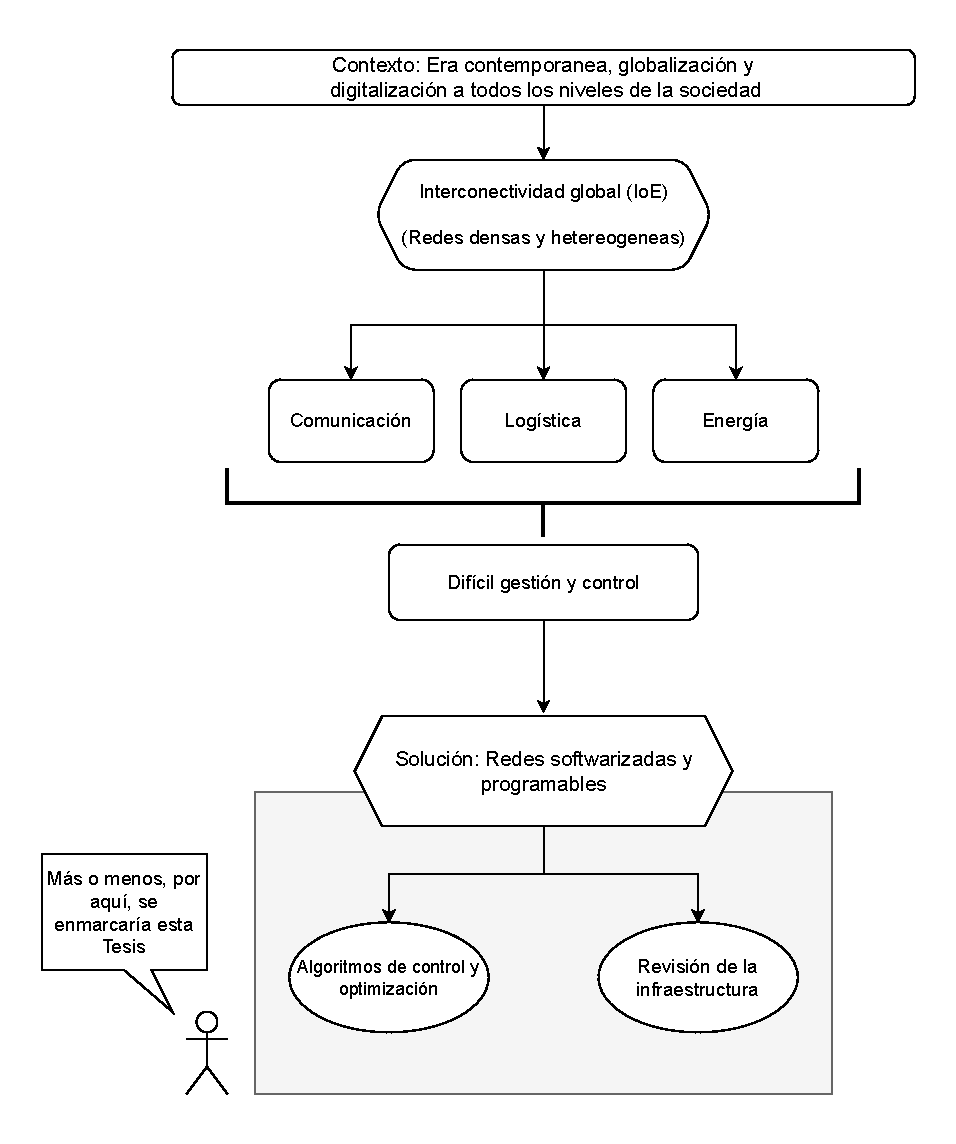
\includegraphics[width=0.85\textwidth]{fig/01_intro/intro_1.drawio.pdf}
    \caption{Diagrama general del marco general de la Tesis}
    \label{fig:intro_1}
\end{figure}

\section{Estructura de la tesis}

A continuación, se presenta la estructura general de esta memoria, describiendo brevemente el contenido de cada uno de sus capítulos. El objetivo es ofrecer una visión global del desarrollo de la Tesis, que sirva como guía para el lector y facilite la comprensión del marco completo del trabajo realizado.\\
\\
El primer capítulo ha contextualizado el ámbito de las redes programables y softwarizadas, destacando su relevancia como base tecnológica para la gestión flexible y dinámica de redes heterogéneas. Asimismo, se ha introducido la problemática asociada a la creciente complejidad de las redes actuales, tanto en las redes de comunicaciones, como las de sensores o las redes de distribución energética, y se han formulado los objetivos principales que guían el desarrollo de esta Tesis. Finalmente, el capítulo concluye con una recopilación de las principales contribuciones científicas generadas a lo largo del trabajo.\\
\\
El segundo capítulo se repasan los conceptos fundamentales y el estado del arte que sustentan la Tesis. El capítulo queda organizado en tres bloques principales. En el primero se abordan las redes programables y softwarizadas, partiendo del paradigma \gls{sdn}, describiendo los modelos de control \textit{out-of-band} e \textit{in-band} y realizando un análisis detallado de las propuestas más relevantes en \textit{in-band}. El segundo bloque se dedica a los servicios y tecnologías habilitadoras en redes softwarizadas y heterogéneas bajo la óptica del MCC (del inglés, Management–Control Continuum): aquí se examinan tanto los servicios básicos (arranque, descubrimiento y provisión de canales de control) como los servicios avanzados (gestión y planificación de recursos, optimización y reconfiguración proactiva de la red). Finalmente, el tercer bloque estudia casos de uso representativos en entornos densos y heterogéneos, con especial atención a las \gls{sg} y a las arquitecturas de sensores \gls{iiot}, para mostrar cómo las tecnologías revisadas se aplican y adaptan a escenarios reales.\\
\\
El tercer capítulo se sintetizan y consolidan los huecos identificados en el capítulo de Estado del Arte, con el objetivo de transformar las lecciones aprendidas en un planteamiento claro del problema, y marcar una hoja de ruta clara para la Tesis.\\
\\
En el capitulo X, .....\\
\\
Por último, el capítulo X recoge las conclusiones principales de la Tesis, así como un bloque que describe futuras líneas de investigación en las que se podrá seguir indagando.


\section{Contribuciones}

El trabajo desarrollado en esta Tesis Doctoral ha generado una contribución notable a la comunidad científica, tanto en términos de generación de conocimiento como en su difusión y transferencia. En concreto, se han publicado cuatro artículos en revistas indexadas en JCR, incluyendo una publicación en una revista de alto impacto Q1 y tres en Q2, y otra dos más que está en revisión (Q2). Además, se han presentado cuatro trabajos en conferencias internacionales organizadas por el IEEE, lo que demuestra la solidez y el interés internacional del trabajo. Como parte del compromiso con la divulgación científica, los avances de esta Tesis también han sido compartidos en eventos como las X Jornadas de Jóvenes Investigadores de la Universidad de Alcalá y la 5th EUGLOH Annual Student Research Conference 2024. Cabe destacar, como elemento diferenciador, el reconocimiento al potencial de transferencia tecnológica de los resultados de esta investigación, materializado en la obtención del Primer Premio en el Concurso de Ideas para la Creación de Empresas de Base Tecnológica de la UAH en 2024. Este premio pone de relieve la capacidad de esta Tesis no solo para generar conocimiento científico de calidad, sino también para transformarlo en soluciones con impacto real en la sociedad, alineadas con los principios de innovación y transferencia del sistema universitario.\\
\\
Artículos de revista indexadas de alto impacto :

\begin{enumerate}
    \item Carrascal, D., Rojas, E., Arco, J. M., Lopez-Pajares, D., Alvarez-Horcajo, J., \& Carral, J. A. (2023). A comprehensive survey of in-band control in sdn: Challenges and opportunities. Electronics, 12(6), 1265. (JCR Q2)
    
    \item Rojas, E., Carrascal, D., Lopez-Pajares, D., Alvarez-Horcajo, J., Carral, J. A., Arco, J. M., \& Martinez-Yelmo, I. (2024). A Survey on AI-Empowered Softwarized Industrial IoT Networks. Electronics, 13(10), 1979. (JCR Q2)
    
    \item Carrascal, D., Rojas, E., Carral, J. A., Martinez-Yelmo, I., \& Alvarez-Horcajo, J. (2024). Topology-aware scalable resource management in multi-hop dense networks. Heliyon, 10(18). (JCR Q1)
    
    \item Carrascal, D., Bartolomé, P., Rojas, E., Lopez-Pajares, D., Manso, N., \& Diaz-Fuentes, J. (2024). Fault Prediction and Reconfiguration Optimization in Smart Grids: AI-Driven Approach. Future Internet, 16(11), 428. (JCR Q2)
    
    \item Carrascal, D., Santos, C., Rojas, E., Arco, J. M., Lopez-Pajares, D. \& Rodriguez-Sanchez F. J. (2025). Dynamic Energy Routing Using Tree-Based Topologies with Fast Convergence applied to Meshed Microgrids. IEEE Access (under review). (JCR Q2)

    \item Carrascal, D., Díaz-Fuentes, J., Manso, N., Lopez-Pajares, D., Rojas, E., Savi, M. \& Arco, J. M. (2025). Softwarized Edge Intelligence for Advanced IIoT Ecosystems: A Data-Driven Architecture Across the Cloud/Edge Continuum. Applied Sciences (under review). (JCR Q2)
  
\end{enumerate}

Conferencias internacionales:

\begin{enumerate}
    \item Carrascal, D., Rojas, E., Lopez-Pajares, D., Manso, N., \& Gutierrez, E. (2023, December). A scalable SDN in-band control protocol for IoT networks in 6G environments. In 2023 6th International Conference on Advanced Communication Technologies and Networking (CommNet) (pp. 1-7). IEEE.
    
    \item Rojas, E., Carrascal, D., Lopez-Pajares, D., Manso, N., \& Arco, J. M. (2024, February). Towards ai-enabled cloud continuum for iiot: Challenges and opportunities. In 2024 International Conference on Artificial Intelligence, Computer, Data Sciences and Applications (ACDSA) (pp. 1-6). IEEE.
    
    \item Comeron, R., Rojas, E., Carrascal, D., Alvarez-Horcajo, J., \& Arco, J. M. (2024, October). Multi-hop collaborative edge computing involving constrained IoT devices at the far edge. In 2024 15th International Conference on Network of the Future (NoF) (pp. 22-24). IEEE.
 
    \item Carrascal, D., Rojas, E., Lopez-Pajares, D., Manso, N., Alvarez-Horcajo, J., \& Martinez-Yelmo, I. (2025, March). Softwarized Data-Driven Architecture for Edge Computing IIoT Environments: A Proof of Concept. In 2025 28th Conference on Innovation in Clouds, Internet and Networks (ICIN) (pp. 64-68). IEEE.
    
\end{enumerate}

Actvidades de divulgación:

\begin{enumerate}
    \item Ponentes a las X Jornadas de Jóvenes Investigadores de la UAH, presentando el trabajo titulado ``DEN2NE: origen, presente, ¿y futuro?''.
    
    \item Participación en la 5th EUGLOH Annual Student Research Conference 2024, con el trabajo titulado ``Advancements in Enabling Technologies for Programmable and Software-Defined Networks: Paving the Way to 6G''.
\end{enumerate}

Premios:

\begin{enumerate}
    \item Primer Premio - Concurso de ideas para la creación de empresas de base tecnológica - UAH (Programa propio de investigación y transferencia de la UAH 2024).
\end{enumerate}

% \begin{figure}[ht]
% \centering
% \resizebox{\textwidth}{!}{%
% \begin{tikzpicture}[
%   font=\small,
%   node distance=1.2cm,
%   milestone/.style={rectangle, draw, rounded corners, fill=blue!10, text width=6cm, align=left},
%   conf/.style={rectangle, draw, rounded corners, fill=green!20, text width=6cm, align=left},
%   year/.style={circle, draw, fill=black!10, minimum size=1cm},
%   line/.style={-{Stealth}, thick}
% ]

% % Año 2023
% \node[year] (y2023) {2023};
% \node[milestone, below=of y2023] (j1) {Electronics 12(6):\\ In-band control in SDN (JCR Q2)};
% \node[conf, below=of j1] (c1) {CommNet 2023:\\ Scalable in-band protocol for IoT};

% % Año 2024
% \node[year, right=6.5cm of y2023] (y2024) {2024};
% \node[milestone, below=of y2024] (j2) {Electronics 13(10):\\ AI for Softwarized IIoT (JCR Q2)};
% \node[milestone, below=of j2] (j3) {Heliyon 10(18):\\ Topology-aware resource mgmt (JCR Q1)};
% \node[milestone, below=of j3] (j4) {Future Internet 16(11):\\ Smart Grid fault prediction (JCR Q2)};
% \node[conf, below=of j4] (c2) {ACDSA 2024:\\ Cloud continuum for IIoT};
% \node[conf, below=of c2] (c3) {NoF 2024:\\ Multi-hop edge computing};

% % Año 2025
% \node[year, right=6.5cm of y2024] (y2025) {2025};
% \node[milestone, below=of y2025] (j5) {IEEE Access (under review):\\ Dynamic energy routing (JCR Q2)};
% \node[conf, below=of j5] (c4) {ICIN 2025:\\ Data-driven edge architecture};

% % Flechas desde año a nodos
% \draw[line] (y2023.south) -- (j1.north);
% \draw[line] (j1.south) -- (c1.north);

% \draw[line] (y2024.south) -- (j2.north);
% \draw[line] (y2024.south) -- (j3.north);
% \draw[line] (y2024.south) -- (j4.north);
% \draw[line] (y2024.south) -- (c2.north);
% \draw[line] (y2024.south) -- (c3.north);

% \draw[line] (y2025.south) -- (j5.north);
% \draw[line] (y2025.south) -- (c4.north);

% \end{tikzpicture}%
% }
% \caption{Timeline of scientific contributions (2023–2025): journal publications and international conferences.}
% \label{fig:timeline_papers}
% \end{figure}

\begin{figure}[ht]
\centering
\begin{tikzpicture}[
  font=\small,
  % --- Estilos de los Nodos (ajustados para ser más compactos) ---
  milestone/.style={
    rectangle, 
    draw, 
    rounded corners, 
    fill=blue!10, 
    text width=3.2cm, % Ancho reducido
    align=center,     % Centrado para mejor estética
    minimum height=1.5cm
  },
  conf/.style={
    rectangle, 
    draw, 
    rounded corners, 
    fill=green!20, 
    text width=3.2cm, % Ancho reducido
    align=center,     % Centrado
    minimum height=1.5cm
  },
  year/.style={
    circle, 
    draw, 
    thick,
    fill=white, 
    minimum size=1cm
  },
  line/.style={
    -{Stealth[length=2mm]}, 
    thick,
    draw=black!70
  }
]

% ---- EJE PRINCIPAL DE LA LÍNEA DE TIEMPO ----
\draw[very thick, -{Stealth[length=3mm]}] (-0.5,0) -- (14.5,0);

% ---- AÑO 2023 ----
\node[year] (y2023) at (1,0) {2023};
% Nodos con texto simplificado
\node[milestone, above=0.8cm of y2023] (j1) {Electronics\\(JCR Q2)};
\node[conf, below=0.8cm of y2023] (c1) {CommNet 2023};

% ---- AÑO 2024 ----
\node[year] (y2024) at (7,0) {2024};
% Nodos con texto simplificado y espaciado ajustado
\node[milestone, above left=0.6cm and 0.1cm of y2024] (j3) {Heliyon\\(JCR Q1)};
\node[milestone, above right=0.6cm and 0.1cm of y2024] (j2) {Electronics\\(JCR Q2)};
\node[milestone, above=3cm of y2024] (j4) {Future Internet\\(JCR Q2)};

\node[conf, below left=0.6cm and 0.1cm of y2024] (c2) {ACDSA 2024};
\node[conf, below right=0.6cm and 0.1cm of y2024] (c3) {NoF 2024};


% ---- AÑO 2025 ----
\node[year] (y2025) at (13,0) {2025};
% Nodos con texto simplificado
% Dado que hoy es 12 de junio de 2025, el estado "under review" es muy relevante.
\node[milestone, above=0.8cm of y2025] (j5) {IEEE Access \& Applied Sciences\\(JCR Q2)\\ (under review)};
\node[conf, below=0.8cm of y2025] (c4) {ICIN 2025};

% ---- CONEXIONES A LA LÍNEA DE TIEMPO ----
% Conexiones 2023
\draw[line] (y2023) -- (j1.south);
\draw[line] (y2023) -- (c1.north);

% Conexiones 2024
\draw[line] (y2024) -- (j2.south);
\draw[line] (y2024) -- (j3.south);
\draw[line] (y2024.north) .. controls +(0,0.8) and +(0,-0.8) .. (j4.south);
\draw[line] (y2024) -- (c2.north);
\draw[line] (y2024) -- (c3.north);

% Conexiones 2025
\draw[line] (y2025) -- (j5.south);
\draw[line] (y2025) -- (c4.north);


\end{tikzpicture}
\caption{Línea de tiempo de contribuciones científicas (2023–2025): publicaciones en revistas y conferencias internacionales.}
\label{fig:timeline_papers_v3}
\end{figure}
\chapter{Estado del Arte}
\label{ch:sota}

Este capítulo tiene como objetivo principal revisar los conceptos clave y el estado del arte que constituyen la base de esta tesis. Para ello, se ha estructurado el capítulo en tres grandes bloques. En primer lugar, se explorarán las redes programables y softwarizadas partiendo de las redes \gls{sdn}, se seguirá con los algoritmos de red y el uso de la \gls{ai} como tecnologías habilitadoras, y por último, se analizarán diversos casos de uso relevantes que ejemplifican la aplicación práctica de estas tecnologías, como son las \gls{sg} y las redes de sensores \gls{iiot}. 

\section{Las redes \glsentryshort{sdn}}
\label{sec:redes_sdn} 

En este primer bloque se revisan las redes \gls{sdn}, que son la base de las redes programables y softwarizadas. Se explorarán sus características, ventajas y desventajas, así como sus paradigmas de modos de control, según se indicó anteriormente. Además, se analizarán los protocolos y así como los aspectos clave de las vertientes de trabajo del modo de control \textit{in-band}, y cómo podemos explorar dicho modo para favorecer la flexibilidad y control en redes densas y heterogéneas.\\
\\
Las redes definidas por software (\gls{sdn}) representan un nuevo paradigma que rompe con las arquitecturas tradicionales de red. Antes de que apareciera el concepto de \gls{sdn}, como se puede apreciar en la Figura~\ref{fig:sdn_paradigma}, las redes tradicionales solían tener un plano de control unificado en los propios dispositivos, llamado generalmente \textit{Control plane}, en el que se definía la lógica que dictaba cómo se debía llevar a cabo el forwarding de los paquetes, y un plano de datos, conocido como \textit{Data plane}, que se implementaba definiendo su datapath, compuesto por varios bloques de procesamiento para reenviar los paquetes. Ambos planos estarían unificados en un sentido lógico, en un mismo dispositivo. Sin embargo, con la aparición del paradigma de las redes \gls{sdn}, como se muestra en la Figura, los nodos tradicionales de la red verían cómo su plano de control sería delegado a una entidad externa llamada controlador, preserbando su capadicar para manejar los paquetes. En contratste con las arquitecturas tradicionales de la red, donde había que ir configurando equipo a equipo, y donde cada uno de ellos iba a desempeñar una función de red, en las redes \gls{sdn}, el controlador permite configurar y supervisar de manera inteligente el comportamiento de la red a través de aplicaciones software, facilitando una programación flexible y dinámica del entorno de red. Por lo que, aunque se sigan llamando ``switches'' o nodos \gls{sdn}, estos se comportarán según las reglas que le instale el controlador, pudiendo gestionar paquetes como un switch, un router, un firewall, etc. 

\begin{figure}[ht!]
\centering
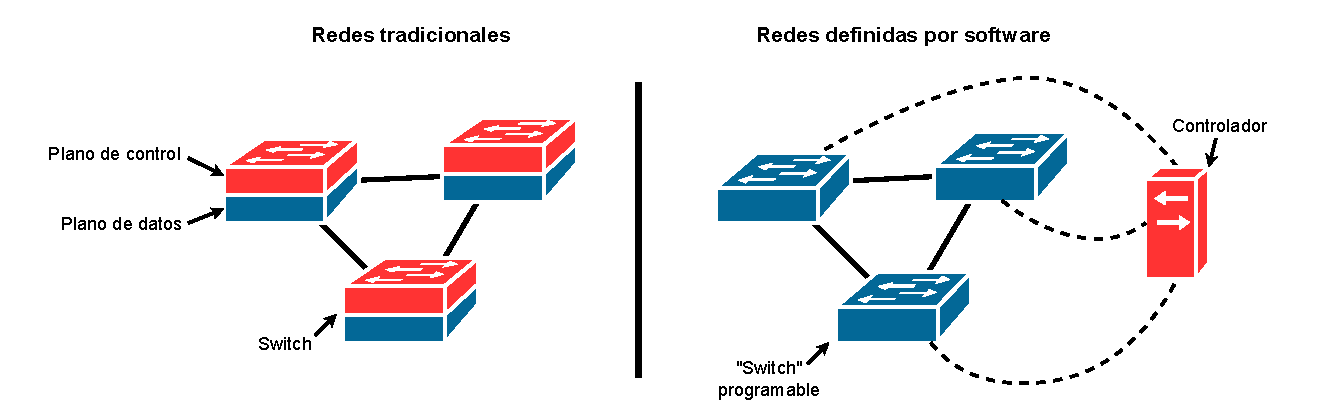
\includegraphics[width=\textwidth]{fig/02_sota/sota_1_sdn_idea.drawio.pdf}
\caption{Paradigma en las redes \glsentryshort{sdn}}
\label{fig:sdn_paradigma}
\end{figure}

La centralización de la gestión simplifica notablemente las tareas del administrador, al proporcionar una visión global del estado de la red y un punto único desde el cual definir su funcionamiento. A través del controlador, las complejas instrucciones de bajo nivel requeridas por los dispositivos de red tradicionales, como switches y routers, las cuales podían variar en función del fabricante, se abstraen mediante interfaces con sintaxis intuitiva, reduciendo la complejidad operativa. Estas capacidades dotan a la red de una gran agilidad y capacidad de adaptación ante cambios o nuevas necesidades, pudiendo conmutar entre distintos perfiles de funcionamiento de forma automática. El simple despliegue de una nueva aplicación sobre el controlador permite modificar de forma coherente el comportamiento de toda la infraestructura, disminuyendo así los costes asociados al mantenimiento, la operación y el despliegue. Además, SDN promueve activamente el uso de soluciones abiertas tanto a nivel de software como de hardware, fomentando ecosistemas interoperables, reduciendo la dependencia de tecnologías propietarias y eliminando barreras de entrada para nuevos actores en el sector.

\subsection{Arquitectura lógica de las redes \glsentryshort{sdn}}
\label{subsec:arquitectura_sdn}

La arquitectura lógica de las redes \gls{sdn} se puede dividir en dos planos, el plano de control y el plano de datos, y además, en tres capas: capa de aplicación, capa de control y capa de infraestructura. En la Figura~\ref{fig:sdn_architecture} se muestra la arquitectura lógica de las redes \gls{sdn}, así como sus interfaces principales de comunicación que más adelante se explicarán.\\
\\
El plano de control, se estructura internamente en dos capas funcionales: la capa de control y la capa de aplicación. Estas se comunican mediante la interfaz norte (northbound interface), que permite a las aplicaciones definir políticas de alto nivel que serán interpretadas y gestionadas por el controlador. Estas capas a menudo se pueden encontrar corriendo en la misma máquina, donde conviven el controlador y las aplicaciones que interactúan con él. Sin embargo, también se puede tener un enfoque distribuido, donde el controlador está en una, máquina, y las aplicaciones en otra, haciendo uso de la interfaz northbound. Por su parte, el plano de datos está conformado por la capa de infraestructura, que engloba los dispositivos físicos de red, principalmente switches \gls{sdn}, responsables del reenvío de paquetes. La interacción entre el plano de control y el plano de datos se realiza a través de la interfaz sur (southbound interface), cuya función es traducir las decisiones del plano de control en instrucciones ejecutables por los dispositivos de red. En este contexto, el controlador actúa como una pieza clave del sistema, asumiendo responsabilidades esenciales como la instalación de reglas de encaminamiento, la monitorización continua del estado de la red y la recopilación de métricas operativas, las cuales serán aprovechadas por todas las aplicaciones que se ejecuten sobre el controlador.

\begin{figure}[ht!]
\centering
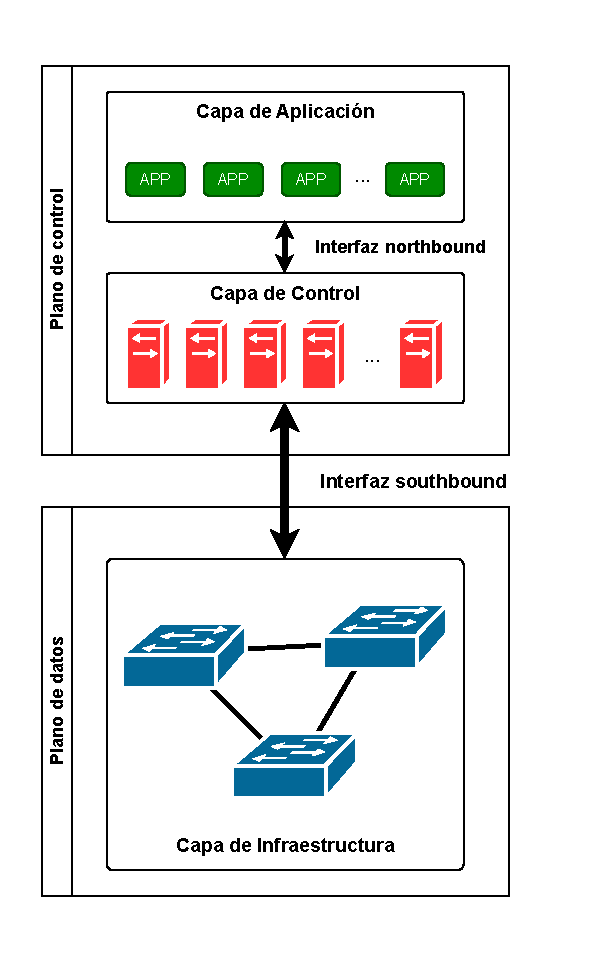
\includegraphics[width=0.5\textwidth]{fig/02_sota/sota_2_sdn_arch_b.drawio.pdf}
\caption{Arquitectura lógica de las redes \glsentryshort{sdn}}
\label{fig:sdn_architecture}
\end{figure}

El plano de datos, por el contrario, no posee lógica de control propia, limitándose a ejecutar las reglas recibidas, como por ejemplo, hacer un reenvío, o descartar paquetes según las reglas establecidas, además de  enviar estadísticas de tráfico al controlador. Esta separación de funciones establece una división clara entre la inteligencia de la red, localizada en el plano de control, y su ejecución, delegada como se ha explicado, al plano de datos. De esta manera, se rompe con el modelo tradicional en el que ambos planos coexistían en un mismo dispositivo de red. Este enfoque modular no solo mejora la escalabilidad y la flexibilidad del sistema, sino que también reduce significativamente los costes de despliegue (\gls{capex}) y operación (\gls{opex}), al concentrar los recursos de cómputo en un nodo centralizado, y simplificar el hardware requerido en los dispositivos de reenvío.\\
\\
Según se ha visto en la Figura~\ref{fig:sdn_architecture}, la arquitectura \gls{sdn} se apoya en una estructura jerárquica formada por tres capas principales: aplicación, control e infraestructura. La capa de aplicación representa el nivel de mayor abstracción dentro del ecosistema \gls{sdn}. Esta capa integra un conjunto de aplicaciones que, apoyándose en los servicios ofrecidos por la capa de control, permiten definir políticas de gestión, \gls{qos}, optimizar el rendimiento de la red y adaptarla dinámicamente a diferentes contextos operativos. Un ejemplo típico de uso es la utilización los servicios de descubrimiento topológico proporcionados por la capa de control, que permiten a las aplicaciones calcular rutas óptimas entre dispositivos de red. Estas aplicaciones suelen desarrollarse empleando lenguajes de alto nivel como Python, Go o C++, con el objetivo de facilitar su portabilidad entre plataformas y maximizar la reutilización del código. No obstante, en la práctica, la existencia de \glspl{api} y entornos de desarrollo específicos para cada plataforma de control, como ONOS, OpenDaylight, Ryu o el nuevo controlador del ecosistema \gls{sdn}, TeraflowSDN, introduce ciertos desafíos en la interoperabilidad y portabilidad del software entre distintas implementaciones. En este sentido, uno de los principales retos actuales de \gls{sdn} sigue siendo la estandarización de interfaces northbound que permitan una integración más fluida y flexible entre aplicaciones y controladores heterogéneos.\\
\\
Descendiendo, la siguiente capa es la capa de control, la cual constituye el núcleo funcional del paradigma \gls{sdn}, albergando la inteligencia centralizada de la red. Actúa como intermediario entre las aplicaciones de alto nivel y los dispositivos físicos de la capa de infraestructura, orquestando tareas críticas como el encaminamiento de flujos, la detección y resolución de fallos, la supervisión continua del estado de la red y la gestión de políticas de seguridad y \gls{qos}. Su papel como middleware se traduce en la capacidad de transformar políticas abstractas generadas en la capa de aplicación en instrucciones simples y concretas que pueden ser entendidas por los nodos \gls{sdn}. Esta capacidad de traducir y escalar la lógica de red permite que un único controlador gobierne cientos o miles de switches de forma eficiente, garantizando escalabilidad y consistencia en entornos distribuidos. Por último, la capa de infraestructura, por su parte, está compuesta por los elementos físicos de la red, fundamentalmente nodos \gls{sdn}, que ejecutan las decisiones tomadas por el plano de control. Estos dispositivos, carentes de lógica propia, cuentan con un agente \gls{sdn} encargado de comunicarse con el controlador a través de la interfaz sur (southbound interface), como por ejemplo, OpenFlow o P4Runtime. Su funcionalidad se reduce al reenvío y descarte de paquetes o la recolección de estadísticas, lo que permite simplificar su diseño y reducir sus requisitos hardware.\\
\\
En cuanto a las interfaces, hay dos, como se ha mencionado anteriormente, la interfaz northbound y la interfaz southbound. La interfaz northbound constituye el canal de comunicación entre la capa de control y la capa de aplicación. Su principal función es ofrecer un punto de acceso lógico al administrador de red, permitiéndole supervisar, configurar y gestionar el comportamiento de la red sin necesidad de interactuar directamente con los mecanismos de bajo nivel que gobiernan los dispositivos físicos. A través de esta interfaz, las aplicaciones pueden programar políticas o solicitudes que serán traducidas por el controlador en instrucciones comprensibles para los elementos de la infraestructura. No obstante, a diferencia de la interfaz southbound, la interfaz northbound carece de una estandarización formal. En consecuencia, la naturaleza y funcionalidad de esta interfaz varían considerablemente en función del controlador \gls{sdn} empleado, cada uno de los cuales suele ofrecer su propia \gls{api} con diferentes modelos de datos, protocolos y lenguajes de interacción.\\
\\
La interfaz southbound constituye el enlace entre la capa de control y la capa de infraestructura dentro de una arquitectura \gls{sdn}. A diferencia de la interfaz northbound, esta sí cuenta con protocolos estandarizados ampliamente adoptados, que permiten la interoperabilidad entre los controladores y los dispositivos de red. Históricamente, el protocolo más representativo ha sido Openflow~\cite{mckeown2008openflow}. En la implementación del protocolo Openflow según se indica en la Figura~\ref{fig:sdn_openflow}, el concepto central es el de flujo (del inglés, \textit{flow}), entendido como un conjunto de paquetes que cumplen determinadas condiciones definidas por el controlador. Estas condiciones se almacenan en las denominadas tablas de flujo (del inglés, \textit{flow tables}), y suelen hacer referencia a valores específicos de campos en la cabecera del paquete o al puerto de entrada por el que se ha recibido.

\begin{figure}[ht!]
\centering
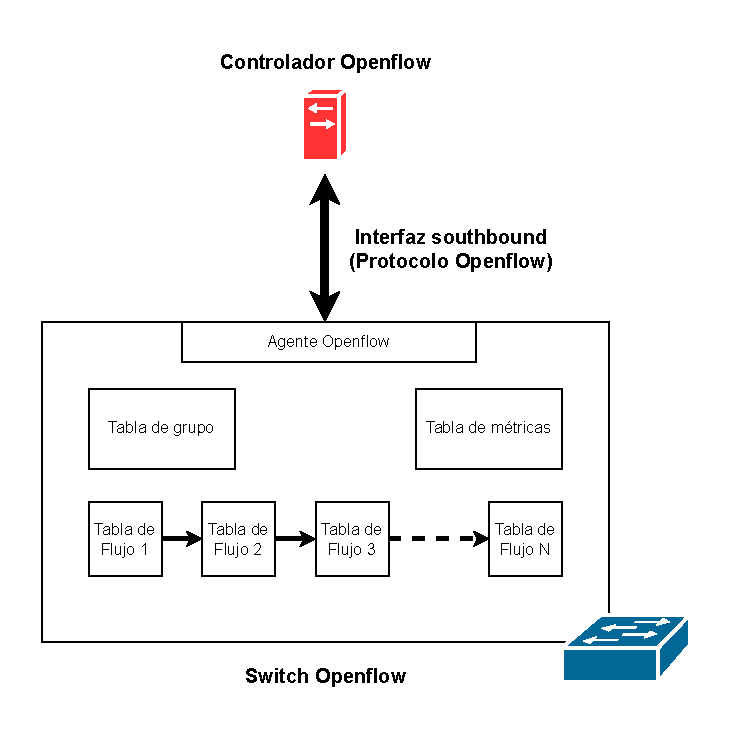
\includegraphics[width=0.7\textwidth]{fig/02_sota/sota_3_sdn_openflow.drawio.pdf}
\caption{Arquitectura básica de switch OpenFlow}
\label{fig:sdn_openflow}
\end{figure}

Cuando un paquete llega a un switch Openflow, empieza a atravesar de forma iterativa las tablas de flujo y cuando este coincide con los criterios de una regla definida en una tabla, se produce una coincidencia (del inglés, \textit{match}), lo que activa un conjunto de instrucciones asociadas a dicha regla. Estas instrucciones pueden incluir el conteo de paquetes, la aplicación de acciones concretas (como reenviar o descartar el paquete), o bien su reenvío hacia otra tabla para un procesamiento adicional. En caso de no darse una coincidencia, se encapsula y se manda al controlador para que este decida que cómo manejarlo. Así, mediante la instalación de estas reglas por parte del controlador \gls{sdn}, se determina el comportamiento de reenvío del switch. La comunicación entre el controlador y los dispositivos se realiza a través de un canal estructurado y seguro, que admite mensajes del controlador al switch, mensajes asíncronos generados por los dispositivos, y mensajes simétricos intercambiables por ambas partes, permitiendo una gestión eficiente y dinámica del estado de red.\\
\\
No obstante, las limitaciones de flexibilidad, extensibilidad y adaptación a nuevas arquitecturas han motivado el surgimiento de alternativas a Openflow. Un ejemplo destacado es el lenguaje \gls{p4}~\cite{bosshart2014p4}, diseñado específicamente para superar las restricciones de OpenFlow. Una de las mayores restricciones que tiene OpenFlow es la especificación de forma explícita de los campos de cabecera sobre los que opera. Estos campos de cabecera han pasado de 12 a 41 campos de cabeceras entre sus versiones 1.0 y 1.5 como se puede ver en la Tabla~\ref{tab:openflow_versions}. Esta evolución ha incrementado la complejidad del protocolo sin proporcionar la flexibilidad necesaria para incorporar nuevas cabeceras o funcionalidades emergentes. 

\begin{table}[ht!]
\centering
\begin{tabular}{|c|c|l|}
\hline
\textbf{Versión} & \textbf{Fecha} & \textbf{Campos de cabecera} \\ \hline
OF 1.0 & Dic. 2009 & 12 campos (Ethernet, TCP/IPv4) \\ \hline
OF 1.1 & Feb. 2011 & 15 campos (MPLS, metadatos entre tablas) \\ \hline
OF 1.2 & Dic. 2011 & 36 campos (ARP, ICMP, IPv6, etc.) \\ \hline
OF 1.3 & Jun. 2012 & 40 campos \\ \hline
OF 1.4 & Oct. 2013 & 41 campos \\ \hline
OF 1.5 & Mar. 2015 & 44 campos \\ \hline
\end{tabular}
\caption{Evolución de versiones del protocolo Openflow y el número de campos de cabecera soportados}    
\label{tab:openflow_versions}
\end{table}

En respuesta a ello, \gls{p4} nació con tres objetivos principales: 

\begin{itemize}
    \item Permitir la reconfiguración del dispositivo en caliente, es decir, cambiar el comportamiento de los switches una vez desplegados.
    
    \item Ofrecer independencia de protocolo, desvinculando el procesamiento de paquetes de protocolos específicos que tengan que estar estandarizados para poder ser gestionados.
    
    \item Proporcionar independencia del hardware, permitiendo que las funcionalidades de procesamiento se definan sin depender de los detalles del dispositivo subyacente. Si bien es cierto que la iniciativa de \gls{p4} nació con este objetivo en mente (\textit{open-hardware}), la realidad es que, en la actualidad, se ha visto como cada fabricante ha implementado equipos que si cumplen con algunas de las arquitecturas de \gls{p4}, pero que cada uno te ofrece unas primitivas de programación diferentes, haciendo que un programa \gls{p4} que corre en un dispositivo de un fabricante no sea totalmente compatible en otro~\cite{hauser2023survey}. 
\end{itemize}

En comparación con Openflow, si nos fijamos en la Figura~\ref{fig:sdn_p4}, podemos apreciar que empleando \gls{p4} se puede definir el cómo el switch va a manejar los paquetes, como los va a procesar y parsear, manteniendo la lógica de las tablas de flujo que teníamos en Openflow, pero ganando en flexibilidad dado que se pueden definir el propio datapath del dispositivo sin depender de un conjunto estandarizado de campos de cabecera. Esto incluso permite que \gls{p4} pueda ser implementado en dispositivos de baja capacidad~\cite{carrascal2020analysis}, al poder ajustar el datapath a la mínima expresión necesaria para cumplir con las necesidades de la red. Al igual que en Openflow se tenía el protocolo de comunicación para la interfaz southbound, \gls{p4} también tiene su propia interfaz de comunicación, llamada P4Runtime~\cite{p4runtime2023}, que permite a los controladores gestionar y programar dispositivos \gls{p4} de forma dinámica. 

\begin{figure}[ht!]
\centering
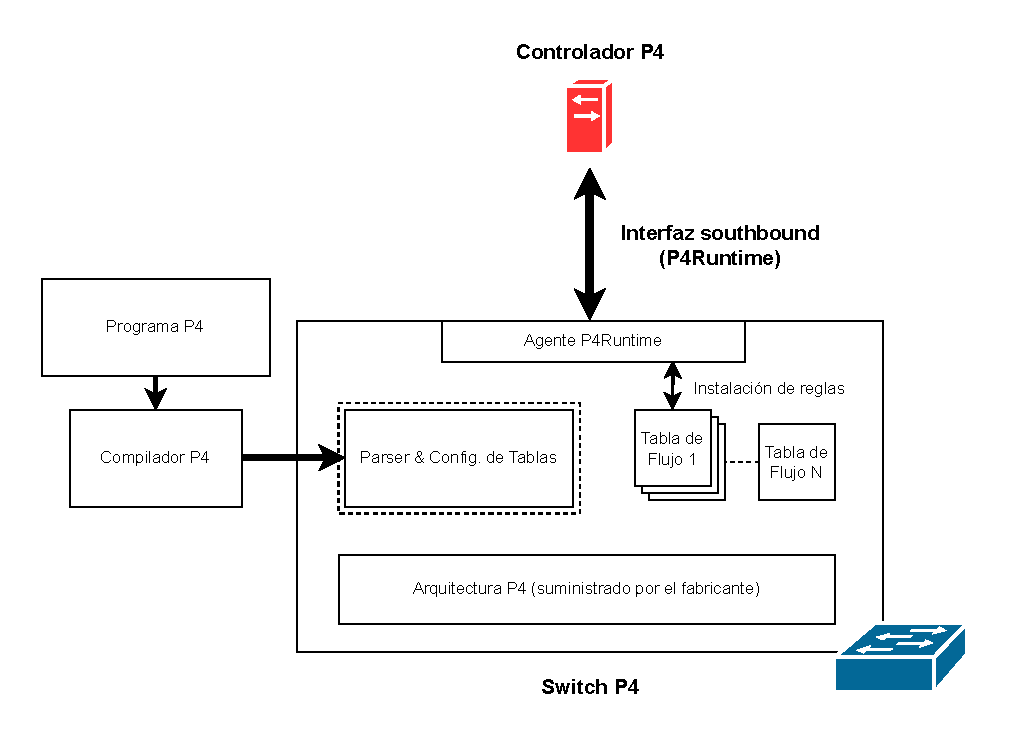
\includegraphics[width=0.9\textwidth]{fig/02_sota/sota_4_sdn_p4.drawio.pdf}
\caption{Arquitectura básica de switch \glsentryshort{p4}}
\label{fig:sdn_p4}
\end{figure}

A diferencia de Openflow, que define un conjunto cerrado de operaciones y estructuras, \gls{p4} y su interfaz P4Runtime introducen la posibilidad de reconfigurar dinámicamente el comportamiento del plano de datos mediante descripciones personalizadas del procesamiento de paquetes. Esto se logra mediante una arquitectura basada en \gls{grpc}, que ofrece cinco tipos de operaciones principales (Write, Read, Set/GetForwardingPipelineConfig y StreamChannel) para gestionar tanto el estado como la lógica interna de los switches programables. De esta forma, \gls{p4} se presenta como una propuesta de evolución de Openflow, orientada a lograr una programabilidad del plano de datos más flexible y escalable, haciéndolo ideal para testing y pruebas de concepto de nuevas soluciones de red.\\
\\
Paralelamente, ha ido creciendo otra vía complementaria orientada a la gestión y configuración unificada de dispositivos de red llamada OpenConfig. Esta iniciativa, impulsada mayormente por un consorcio de operadores y fabricantes, propone un conjunto de modelos de datos basados en YANG que permiten describir de forma estandarizada y agnóstica el estado operativo y la configuración de dispositivos de red. A diferencia de OpenFlow o P4Runtime, que se centran en el comportamiento del plano de reenvío, OpenConfig aborda la gestión, configuración, el monitoreo y la automatización de tareas de red a través de protocolos como gNMI o NETCONF. Esto convierte a OpenConfig una herramienta clave para aquellas empresas que buscan una gestión softwarizada y programable de sus infraestructuras ya existentes, dado que permite la integración de dispositivos heterogéneos de diferentes fabricantes bajo un modelo común de gestión. Si bien es cierto que OpenConfig no permite definir explícitamente el plano de datos, a diferencia de Openflow o \gls{p4}, donde se considera que todos los switches o nodos \gls{sdn} equivalen a un único dispositivo lógico gestionado de forma centralizada, OpenConfig propone un enfoque diferente. Esta iniciativa busca establecer un conjunto común de modelos de datos y configuración, independientes del fabricante, para gestionar redes heterogéneas. A diferencia del enfoque \gls{sdn} tradicional, en el que los dispositivos se integran como un único plano de control y datos, los dispositivos gestionados mediante OpenConfig siguen operando como entidades independientes. Ambos enfoques persiguen una mayor transparencia y facilidad de gestión de la red, pero difieren en su grado de abstracción y centralización: mientras \gls{sdn} trata la red como un todo unificado, OpenConfig mantiene la identidad individual de cada dispositivo, facilitando la interoperabilidad en entornos mixtos. Sin embargo, los últimos controladores \gls{sdn} como TeraflowSDN~\cite{teraflowsdn2021}, han comenzado a integrar OpenConfig como una de sus interfaces southboud (además de \gls{p4}), incluso llegando a no implementar Openflow, lo que sugiere una tendencia hacia un nuevo ecosistema de redes \gls{sdn} que combina la flexibilidad de la programación del plano de datos con la estandarización y la gestión eficiente de dispositivos heterogéneos.\\
\\
En este sentido, la evolución de la interfaz southbound no debe entenderse en términos de sustitución de unos protocolos por otros, sino como una diversificación funcional que permite combinar capacidades de reenvío programable, comunicación eficiente y gestión estandarizada según las necesidades específicas de cada red.


\subsection{Arquitectura física de las redes \glsentryshort{sdn}}
\label{subsec:arquitectura_fisica_sdn}

Una vez que se ha revisado la arquitectura lógica de las redes \gls{sdn}, es importante entender cómo se implementa físicamente esta arquitectura, es decir, cómo se conectan los diferentes componentes que se vienen explicando en la sección anterior.\\
\\
En una red \gls{sdn}, según se indicó en la Figura~\ref{fig:sdn_architecture}, se compone de un elemento central, el controlador, y un conjunto de swicthes o nodos \gls{sdn} distribuidos en la capa de infraestructura los cuales son gestionados por el controlador. Sin embargo, también es posible la implementación de múltiples controladores en una misma red \gls{sdn}, lo cual aporta funcionalidades adicionales a la red, como mecanismos de respaldo y tolerancia a fallos, que incrementan su fiabilidad, y por ende, la resilencia de la red. Por ello, se pueden clasificar las conexiones físicas en las redes \gls{sdn} en dos bloques:  

\begin{itemize}
    \item Las conexiones entre los switches de la capa de infraestructura.
    \item Las conexiones entre el controlador y los switches de la capa de infraestructura.
\end{itemize}
 
Las primeras constituyen la topología física de la red, cuya estructura depende del entorno en el que se despliegue y de los objetivos funcionales de la red. Por ejemplo, en redes \gls{sdn} diseñadas para centros de datos, es común adoptar una arquitectura jerárquica y regular, ya que esta facilita la escalabilidad y permite absorber incrementos en la demanda de tráfico de forma eficiente~\cite{lopez2021nuevos}. En cambio, en entornos de redes de sensores \gls{sdn}, es frecuente emplear topologías en malla parcial (tendiendo hacia a una malla completa)~\cite{baddeley2018evolving}, que permiten una mayor resiliencia frente a fallos y una reducción en la latencia gracias a la existencia de múltiples caminos entre nodos de la topología.\\
\\
En cuanto a las conexiones entre el controlador y los switches de la capa de infraestructura, estas se pueden clasificar en principalmente en dos categorías, si bien es cierto que se puede encontrar una tercera categoría que combina ambas. Observando la Figura~\ref{fig:sdn_control_paradigms}, se pueden distinguir dos paradigmas de control: el modo de control \textit{in-band} y el modo de control \textit{out-of-band}, y por último, el modo de control \textit{hybrid-band}, el cual es una combinación de los dos anteriores. \\

\begin{figure}[ht!]
\centering
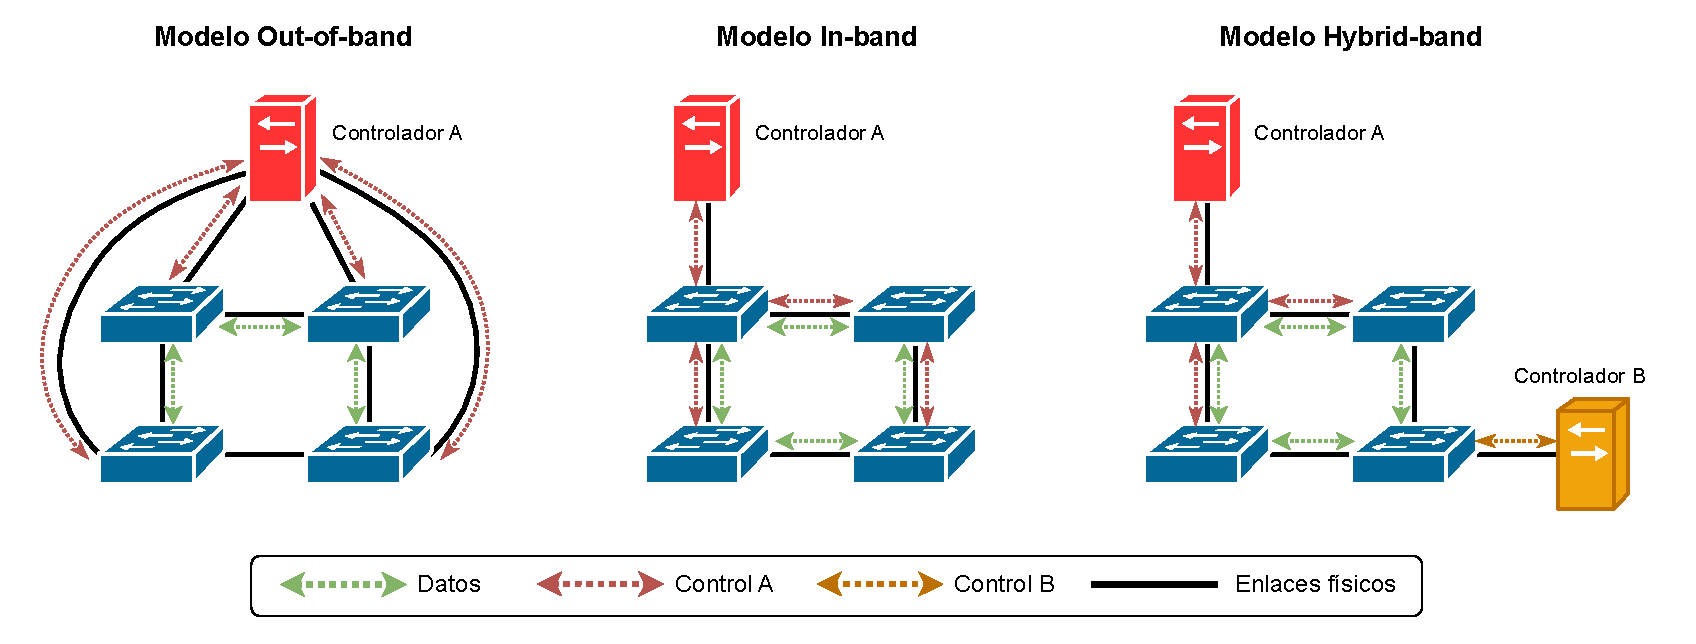
\includegraphics[width=\textwidth]{fig/02_sota/sota_5_sdn_control_paradigms.drawio.pdf}
\caption{Paradigmas de control en las redes \glsentryshort{sdn}}
\label{fig:sdn_control_paradigms}
\end{figure}

Al desplegar el canal de control en una red \gls{sdn}, es posible optar por un enfoque out-of-band o in-band, como se ilustra en la Figura~\ref{fig:sdn_control_paradigms}. En el primer caso, denominado out-of-band, cada nodo \gls{sdn} dispone de un enlace físico dedicado que lo conecta directamente con el controlador. De este modo, la información de control se transmite a través de una red independiente, exclusiva para dicho propósito, lo cual incrementa la seguridad y el aislamiento del canal, aunque implica un mayor coste de infraestructura al requerir al menos un enlace adicional por nodo. Por el contrario, en el enfoque in-band, solo algunos nodos \gls{sdn} mantienen un enlace directo con el controlador, mientras que el resto accede a él a través de la propia red de datos, reutilizando los enlaces existentes para transportar la información de control. En este caso, los mensajes de control comparten la infraestructura del plano de datos, lo que puede comprometer su seguridad e integridad, al estar más expuestos a posibles interferencias o interceptaciones. \\
\\
Finalmente, el enfoque hybrid-band contempla una solución intermedia, en la que coexisten enlaces dedicados y compartidos para la comunicación con el plano de control~\cite{Suo16}, como se muestra en la Figura~\ref{fig:sdn_control_paradigms}. Este modelo busca equilibrar los costes operativos con los requisitos de fiabilidad y seguridad.\\
\\
Cada uno de estos esquemas de despliegue presenta ventajas e inconvenientes~\cite{Suo16}, y la elección entre uno u otro depende fundamentalmente del escenario de red y del caso de uso considerado~\cite{Jalili17,Kafetzis22}. No existe un paradigma mejor que otro, sino, que cada enfoque ofrece características particulares que pueden resultar más o menos adecuadas según los requisitos del entorno. Por ejemplo, el modelo out-of-band requiere un enlace físico adicional dedicado a la comunicación entre el controlador y cada nodo \gls{sdn}, lo que incrementa notablemente los costes de despliegue y mantenimiento. No obstante, esta separación garantiza un mayor aislamiento del canal de control, lo que mejora sustancialmente la seguridad de las comunicaciones. En contraposición, el modelo in-band reutiliza los enlaces existentes del plano de datos para transmitir la información de control, lo que reduce significativamente el coste de infraestructura. Sin embargo, esta economía viene a expensas de una menor seguridad, ya que los mensajes de control comparten canal con el tráfico de red, quedando expuestos a posibles interferencias o ataques. \\
\\
Además, uno de los principales retos del enfoque in-band radica en la configuración inicial, es decir, el nodo debe conocer de antemano la ruta hacia el controlador a través de la red de datos. En contraste, el modelo out-of-band facilita esta tarea, al disponer de una interfaz exclusiva para dicho propósito. Por ello, en in-band, esta información tiene que proporcionarse mediante protocolos específicos que permiten a cada nodo identificar la interfaz adecuada para reenviar los paquetes de control. Estos protocolos son de especial de interés dado que no existe una solución estandarizada en la academia. Debido a lo cual, se quiere explorar en mayor medida qué opciones existen y qué metodologías se han empleado, dado que estas soluciones son fácilmente extrapolables a otros tipos de redes densas y heterogéneas que empleen entornos softwarizados con una tipología de control in-band. Así, por ejemplo, en entornos como el \gls{iot}, donde los dispositivos suelen disponer de una única interfaz de comunicaciones y cuentan con recursos energéticos limitados, el modelo in-band se presenta como una alternativa óptima, al evitar la necesidad de enlaces adicionales que aumentarían el consumo energético y reducirían la vida útil del sensor. \\
\\
La Tabla~\ref{table:inband_adventages} resume comparativamente las principales características de estos modelos. En ella se observa cómo el paradigma out-of-band destaca por su simplicidad de configuración y seguridad, mientras que el in-band sobresale en términos de escalabilidad y costes. 

\begin{table}[ht]
\centering
\resizebox{\textwidth}{!}{%
\begin{tabular}{|l|c|c|}
\hline
\textbf{Propiedad} & \textbf{Control \textit{out-of-band}} & \textbf{Control \textit{in-band}} \\
\hline
Configuración del dispositivo SDN & Sencilla & Compleja \\ \hline
Seguridad del canal de control & Segura, canal aislado & Riesgosa, canal compartido \\ \hline
Costes de mantenimiento y despliegue & Elevados & Reducidos \\ \hline
Escalabilidad & Limitada & Buena \\ \hline
Resiliencia & Costosa & Recuperación rápida\\
\hline
\end{tabular}
}
\caption{Características del control \textit{in-band} y \textit{out-of-band}}
\label{table:inband_adventages}
\end{table}


\subsubsection{Propuestas de despliegue con control in-band}
\label{subsubsec:propuestas_inband}

La tendencia actual indica que el control in-band está ganando protagonismo en los despliegues de redes \gls{sdn}~\cite{Awan19}, especialmente en redes de grandes y densas, donde el coste de utilizar un modelo out-of-band puede resultar prohibitivo. Además, el control in-band habilita el desarrollo de una amplia variedad de nuevas aplicaciones, sobretodo en entornos \gls{sdn} híbridos o con restricciones de recursos~\cite{Khorsandroo21,Rojas21}, donde el despliegue de enlaces dedicados de control puede ser complejo o incluso inviable. Entre los casos de uso más representativos que se benefician del control in-band se encuentran las redes \gls{5g}~\cite{Murtadha21} y las \glspl{ntn}~\cite{Guo21}, así como diversos escenarios del ámbito \gls{iot}, como redes submarinas~\cite{Shi22}, entornos orientados a la eficiencia energética~\cite{Maity22} o sistemas con recursos limitados~\cite{Chattopadhyay19}. A pesar de sus numerosas ventajas, los esfuerzos dirigidos al diseño de protocolos comunes e integrales para el control in-band han sido escasos. Una solución efectiva debería considerar la compatibilidad con plataformas ampliamente utilizadas, tanto en los controladores como en los dispositivos \gls{sdn}, a fin de garantizar una integración completa en los despliegues actuales. En este contexto, diferentes propuestas han explorado mecanismos para habilitar o mejorar el control in-band, con el objetivo de facilitar su adopción en entornos reales y responder a los retos que plantea,este paradigma. A continuación, se presentan algunos de los trabajos más representativos en esta línea.\\
\\
%En este contexto, los trabajos existentes sobre control in-band pueden clasificarse en función de tres aspectos clave que dicho paradigma debería proporcionar: encaminamiento automático, recuperación rápida ante fallos y arranque autónomo de la red. Además, se ha identificado un cuarto aspecto transversal, relacionado con entornos de control distribuido que tambien merece la pena revisar. En primer lugar, la necesidad de contar con un mecanismo de encaminamiento automático en el control in-band resulta evidente. Mientras que el modelo out-of-band suele implementarse mediante enlaces directos entre los nodos \gls{sdn} y el controlador, el control in-band requiere calcular rutas entre los dispositivos de red y uno o varios controladores, tanto en un sentido ascendente, como descendente. Este mecanismo de encaminamiento es esencial para permitir la comunicación de control a través del plano de datos y suele condicionarse al tipo de despliegue o a las capacidades del entorno. En segundo lugar, una de las principales ventajas del control in-band es su capacidad de recuperación rápida ante fallos. En caso de que un enlace o switch sufra una avería, es posible restaurar la comunicación de control simplemente seleccionando una ruta alternativa dentro del plano de datos. No obstante, para que este proceso resulte eficaz, los mecanismos de restauración o protección de rutas deben estar bien definidos y coordinados con la lógica de encaminamiento previamente establecida. El tercer aspecto fundamental es el denominado arranque autónomo de la red (del inglés, \textit{network bootstrapping}), que hace referencia a la capacidad del sistema para configurar automáticamente los parámetros necesarios antes del inicio de su operación. Estos parámetros incluyen, entre otros, la información de conectividad entre nodos \gls{sdn} y controladores. Si bien este proceso también es deseable en entornos out-of-band, en el caso de control in-band se convierte en un requisito crítico, ya que las rutas de control pueden variar en función del despliegue y del protocolo de encaminamiento utilizado. Por último, en entornos con control distribuido, donde existen varios controladores implicados en la toma de decisiones, es necesario incorporar mecanismos de coordinación que permitan compartir rutas, realizar recuperación ante fallos de manera conjunta y gestionar el arranque de la red de forma sincronizada. Además, el control in-band puede ofrecer un canal adicional para la comunicación interna entre controladores, lo cual añade una dimensión interesante a su uso en arquitecturas distribuidas.\\
%\\

%En primer lugar, varios autores han sentado las bases de un marco genérico de control in-band y han explorado mecanismos de recuperación ante fallos simples. Sharma et al.\cite{Sharma16} presentan un prototipo basado en OpenFlow y NOX que evalúa la viabilidad de este paradigma en distintos switches, proponiendo métodos de restauración y protección frente a fallos individuales. De manera similar, Goltsmann et al.\cite{Goltsmann17} introducen el protocolo ICS, que construye un árbol de expansión etiquetado para garantizar conectividad resiliente con bajo sobrecoste. Ambos trabajos ponen de manifiesto la factibilidad del control in-band en escenarios sencillos, pero no extienden sus propuestas a la gestión simultánea de múltiples fallos ni proporcionan un estándar interoperable.

%Un segundo bloque de investigaciones se centra en la tolerancia a múltiples fallos y en la complejidad de su implementación práctica. Khakhalin et al.\cite{Khakhalin17} formulan un algoritmo resistente a múltiples averías mediante la asignación de etiquetas únicas a cada switch, aunque la gestión de estas etiquetas se complica rápidamente en redes de gran escala. Por su parte, Mohan et al.\cite{Mohan18} definen un esquema de rutas de control disjuntas por nodo para detectar y aislar switches maliciosos; si bien mejora la seguridad, su formulación matemática no escala bien debido al elevado número de variables de decisión.

%Un tercer grupo aborda la disponibilidad del canal y el arranque autónomo de la red. Raza et al.\cite{Raza17} y González et al.\cite{Gonzalez18} investigan el uso de \gls{mptcp} para aumentar la tolerancia de rutas, aunque ambos dependen de un enlace out-of-band inicial para la fase de arranque. Fan et al.~\cite{Fan20}, por su parte, diseñan un algoritmo centralizado que ubica el canal in-band en el enlace con mayor ancho de banda disponible, mejorando métricas como RTT y PLR en topologías tipo Fat-Tree; no obstante, su solución no se ha validado en redes genéricas de gran tamaño.

%Finalmente, existen propuestas más avanzadas y específicas para entornos heterogéneos. Görkemli et al.\cite{Gorkemli18} plantean un plano de control dinámico capaz de redistribuir carga entre varios controladores y adaptar el enrutamiento in-band según la topología y las necesidades de las aplicaciones; sin embargo, su evaluación solo contempla despliegues virtualizados. Holzmann et al.\cite{Holzmann19} presentan Izzy, un protocolo distribuido basado en árboles de expansión y direcciones temporales que logra tiempos de recuperación inferiores a 100 ms en simulaciones WAN de 100 nodos, aunque aún no dispone de validación en entornos reales. En el ámbito de redes satelitales, Ningyuan et al.\cite{Ningyuan21} proponen una arquitectura de doble capa para constelaciones \gls{leo}, que garantiza rutas fiables pese a la movilidad de los satélites, si bien su propuesta permanece en fase de simulación. Por último, Kumazoe et al.\cite{Kumazoe22} diseñan un canal in-band en entornos \gls{p4}, embebiendo mensajes de control en paquetes de usuario; aunque innovador, su evaluación inicial revela degradaciones en el reenvío de datos que quedan pendientes de resolver.




\section{Algoritmos de red y \glsentryshort{ai}}
\label{sec:tecnologias_habilitantes}

En este segundo bloque se quieren revisar las principales tecnologías habilitantes que permiten la creeación, control y gestión de las redes programables y softwarizadas. Estas tecnologías son fundamentales para entender el marco de trabajo de la tesis, y cómo, posteriormente, se pueden llegar a aplicar a diferentes casos de uso. 


\section{Casos de uso}  
\label{sec:casos_de_uso}
En este último bloque se revisan los casos de uso más relevantes que se pueden encontrar en la literatura. Estos casos de uso son ejemplos prácticos de cómo las tecnologías habilitantes y las redes programables y softwarizadas se aplican en contextos reales, como las \gls{sg} y las redes de sensores \gls{iiot}. 
\chapter{Planteamiento del problema}
\label{ch:problema}

En este capítulo se sintetizan y consolidan los huecos identificados en el capítulo de Estado del Arte, con el objetivo de transformar las lecciones aprendidas en un planteamiento claro del problema, y marcar una hoja de ruta clara para la Tesis. Para ello, se recogen las conclusiones parciales ya extraídas en las secciones correspondientes: control \textit{in-band} (Sección~\ref{subsec:conclu_inband}), arranque y provisión de canales de control en entornos densos y heterogéneos (Sección~\ref{subsubsec:conclu_etiquetado}), gestión y planificación de recursos (Sección~\ref{subsubsec:conclu_recursos}), optimización y reconfiguración proactiva (Sección~\ref{subsubsec:conclu_opt}), encaminamiento energético y arquitecturas para \gls{ei}/\glspl{prg}/\gls{sg} (Sección~\ref{subsubsec:conclu_sg}) y arquitecturas inteligentes \gls{iiot} (Sección~\ref{subsubsec:conclu_iiot}).\\
\\
A partir de esa revisión consolidada se extraerán las lecciones aprendidas, los huecos comunes, se priorizarán los retos con mayor impacto práctico, pudiendo sentar las bases de la Tesis. Finalmente, este capítulo presenta la estrategia de trabajo propuesta, y como se han organizado las contribuciones de la Tesis en los siguientes capítulos.\\
\\
Las lecciones extraídas de la revisión sistemática del estado del arte muestran un panorama consistente: existen avances metodológicos y prototipos relevantes en control \textit{in-band}, arranque/etiquetado jerárquico, gestión de recursos, optimización proactiva y arquitecturas \gls{iiot}/\gls{sg}, pero la mayoría de estas aportaciones no resuelven de forma conjunta los requerimientos de despliegue en entornos densos y heterogéneos. En todos los dominios examinados emergen huecos comunes que limitan la adopción práctica: falta de soluciones <<agnósticas>> al dataplane y al proveedor, escasez de protocolos \textit{in-band} estandarizados, ausencia de mecanismos de arranque (\textit{bootstrapping}) seguros y ligeros validados a gran escala, carencia de coordinación eficiente entre controladores distribuidos, y validaciones limitadas sobre hardware real o testbeds representativos. Estas carencias son recurrentes y condicionan tanto la viabilidad técnica como la transferencia de resultados a escenarios reales (\gls{iiot}, micro-redes, smart grids).\\
\\
Del análisis por áreas concretas se obtienen conclusiones operativas que permiten priorizar líneas de trabajo. En el ámbito del arranque y provisionamiento de canales de control, el etiquetado jerárquico y las construcciones modo árbol enraizadas emergen como la técnica más prometedora: reducen estado local, permiten encaminamiento con bajo coste y facilitan el diseño de rutas de control compactas. No obstante, muchas propuestas actuales (Torii/\gls{ga3}/eTorii, Amaru, IoTorii, Izzy, etc.) están validadas en topologías homogéneas o en simulación y/o requieren modificaciones del dataplane; pocas consideran nativamente heterogeneidad de enlaces, nodos con recursos muy limitados (a excepción de IoTorii) o escenarios multi-raíz con coordinación entre controladores. En gestión y planificación de recursos, la tensión centralización contra distribución es clave. Los esquemas centralizados facilitan optimización global pero fallan en escalabilidad y resiliencia; los distribuidos ganan en tolerancia y reparto de carga, pero sufren mayor complejidad, tiempos de convergencia más grandes y visibilidad parcial de la red. Aquí el etiquetado jerárquico puede actuar como palanca técnica: al simplificar la topología física a la topología lógica, se reduce señalización y habilita decisiones locales eficientes, lo que hace posibles diseños distribuidos más prácticos. En optimización y reconfiguración proactiva (tanto para \gls{sg} como para redes \gls{iiot}), los enfoques existentes (optimizadores exactos, metaheurísticos y modelos \gls{ai}/\gls{ml}) demuestran potencial, pero tropiezan con problemas reales: modelos no agnósticos (entrenados para una topología concreta), elevada señalización o coste computacional para nodos con recursos limitados, y validaciones insuficientes con datos reales o testbeds. Finalmente, en \gls{iiot} las arquitecturas muestran avances (\textit{edge/fog}, microservicios, federated learning, etc.), pero muchas implementaciones son cerradas o no escalan en despliegues de alta densidad; falta un framework de orquestación que conecte inferencia en tiempo real con reconfiguración automática, y es necesario abordar la autoscalabilidad, latencia y seguridad desde el diseño. En el ámbito del encaminamiento energético y las arquitecturas para el \gls{ei} pone de manifiesto avances relevantes, sin embargo, la mayoría de las propuestas analizadas descansan en optimizaciones estáticas o en soluciones centralizadas, lo que reduce su capacidad de adaptación y escalabilidad frente a escenarios dinámicos; son escasas las aproximaciones que exploten topologías multi-raíz con decisión autónoma a nivel de nodo; no existe consenso sobre criterios de selección de rutas que equilibren simultáneamente minimización de pérdidas, balance local y resiliencia.\\
\\
A partir de esos \textit{gaps}, la hoja de ruta de la Tesis articula unas líneas de investigación concretas, metodológicamente acotadas y alineadas con los dos bloques de objetivos previamente definidos.

\begin{itemize}
    \item En primer lugar, se plantea diseñar y formalizar esquemas de etiquetado jerárquico con las siguientes propiedades: (i) <<agnosticismo>> frente a heterogeneidad de enlace (capacidad/latencia) y a implementaciones de \textit{dataplane legacy}; (ii) mínima o nula necesidad de modificar el hardware/software de reenvío; (iii) soporte para multi-raíz y coordinación eficiente entre controladores distribuidos; (iv) reducción de señalización mediante decisiones locales informadas (posiblemente asistidas por modelos \gls{ai}/\gls{ml} compactos); y (v) capacidad de reconfiguración de la red proactivamente (rutas de respaldo). Estas contribuciones atacan directamente el primer bloque de objetivos, proporcionando los bloques de arranque, encaminamiento y reconfiguración de baja sobrecarga necesarios para operar en topologías reales, densas y heterogéneas.

    \item En segundo lugar, la Tesis investigará estrategias híbridas de gestión y orquestación de recursos que combinen optimización centralizada (cuando la latencia y la capacidad de señalización lo permitan) con decisiones locales ligeras basadas en el etiquetado jerárquico. En la práctica esto implica diseñar protocolos jerárquicos de coordinación, políticas de delegación de decisiones (qué se decide localmente y qué se delega al controlador), y mecanismos de retroalimentación que permitan al plano de control incorporar información sin sobrecargar la red. 

    \item En tercer lugar, la Tesis se plantea diseñar una arquitectura \gls{iiot} inteligente, con marcos de orquestación unificados que integren salidas de inferencia (\gls{ai}/\gls{ml}) en tiempo real de telemetría de los sensores para desencadenar reconfiguraciones dinámicas de red, reubicación de servicios y mantenimiento preventivo. Además, se debe respetar el prototipado abierto y reproducible de microservicios, y pipelines de inferencia con autoescalado. Otro aspecto importante es la evaluación de cuellos de ingestión de datos y la incorporación de mecanismos ligeros de autenticación y trazabilidad de decisiones para proteger el despliegue de la arquitectura. Estas tareas responden a los \textit{gaps} detectados en las arquitecturas \gls{iiot} (ausencia de implementaciones abiertas, carencia de orquestación basada en inferencia en tiempo real, y limitaciones en autoscalado).
\end{itemize}

Metodológicamente, la Tesis combinará análisis teórico, simulación/emulación y prototipado práctico. El plan experimental incluye:

\begin{enumerate}
    \item Validaciones por simulación/emulación en topologías heterogéneas y densas, donde, se emplearán topologías aleatorias, densas, e hiperconectivas. Se hará uso del generador de topologías aleatorias conocido como \gls{brite}~\cite{brite}.

    \item Validación real cuando se tengan las capacidades hardware de llevarlo a cabo.

    \item Experimentos en testbeds representativos. En caso de trabajar  con las \gls{sg}, se emplearán benchmarks \gls{ieee} para feeders. En el caso de despliegues de arquitecturas \gls{iiot}, se empleará el CPD de la universidad para emular la visión continua de factory/edge/cloud. 

\end{enumerate}


En resumen, la Tesis propone una agenda integradora: avanzar en mecanismos prácticos de control \textit{in-band} y etiquetado jerárquico (soporte multi-raíz), desarrollar estrategias de orquestación híbrida que combinen decisión local y optimización global, integrar \gls{ai}/\gls{ml} de forma eficiente y portable para asistencia en la toma de decisiones, y validar todo ello mediante prototipos abiertos y experimentación en escenarios representativos (\gls{iiot}, \gls{sg} y micro-redes). Estas líneas están alineadas de forma directa con los dos grandes bloques de objetivos de la Tesis: (i) profundizar en mecanismos de control para redes programables y su extensión a \gls{iiot} y redes de distribución eléctrica; y (ii) estudiar y construir infraestructuras software de despliegue, monitorización, orquestación y seguridad que permitan la toma de decisiones automáticas y robustas en entornos reales y heterogéneos. Estas lineas de trabajo se presentarán a continuación, de forma secuencial y cronológica (en la medida de lo posible), organizando las propuestas/publicaciones realizadas en diferentes capítulos. 



\chapter{Propuesta escalable de control In-band para entornos inalámbricos y de baja capacidad}
\label{ch:propuestaInband}

En este capítulo se presenta la primera aportación de la Tesis: una propuesta de control \textit{in-band} escalable para redes \gls{sdn} en entornos inalámbricos y de baja capacidad, concebida en el marco de los futuros ecosistemas \gls{6g}. El origen de esta línea de trabajo se remonta a mi Trabajo Fin de Máster~\cite{carrascal2023diseno}, donde se sentaron las primeras bases conceptuales. Posteriormente, se consolidó mediante el desarrollo y publicación de una revisión sistemática sobre los mecanismos de control \gls{sdn} \textit{in-band}~\cite{carrascal2023comprehensive}, y materializó como primera contribución de la Tesis en forma de ponencia en la conferencia CommNet 2023~\cite{carrascal2023scalable}. Aunque la evaluación experimental de esta propuesta se planteó principalmente como una prueba de concepto y, por tanto, no resulta exhaustiva, constituye un punto de partida sólido que guía y fundamenta las siguientes contribuciones de la Tesis.

\section{Introducción}

Los recientes avances en comunicaciones móviles, junto con la mejora de las capacidades de hardware, han impulsado el crecimiento del \gls{iot} al interconectar miles de millones de objetos mediante comunicaciones \gls{m2m} en entornos tanto domésticos como industriales~\cite{Balaji2019}. Puede afirmarse sin lugar a dudas que el \gls{iot} forma parte integral del Internet presente y futuro: ha transformado la forma en que interactuamos con el entorno, permitiendo la interconexión autónoma de dispositivos a través de la red y ofreciendo entornos inteligentes y adaptativos que responden a las necesidades de la sociedad. No obstante, el crecimiento exponencial de dispositivos \gls{iot} conectados a redes móviles introduce nuevas exigencias en términos de capacidad, rendimiento, latencia y eficiencia de red que deben abordarse (Ver Figura~\ref{fig:in_band_1}). La tecnología \gls{5g} se propuso y desplegó comercialmente para cubrir muchos de los requisitos de las redes \gls{iot} y sus aplicaciones. Sin embargo, con la rápida proliferación de nuevos sensores y la consiguiente expansión de las redes \gls{iot}, los requisitos técnicos necesarios para sostener los entornos tradicionales \gls{m2m} (plenamente autónomos, dinámicos e inteligentes) se han incrementado. Por tanto, se requiere una tecnología más avanzada para satisfacer las demandas futuras de las redes \gls{iot}, y la arquitectura \gls{6g} se postula como una solución capaz de afrontar estos nuevos retos~\cite{Nguyen2022}.

\begin{figure}[ht!]
   \centering
    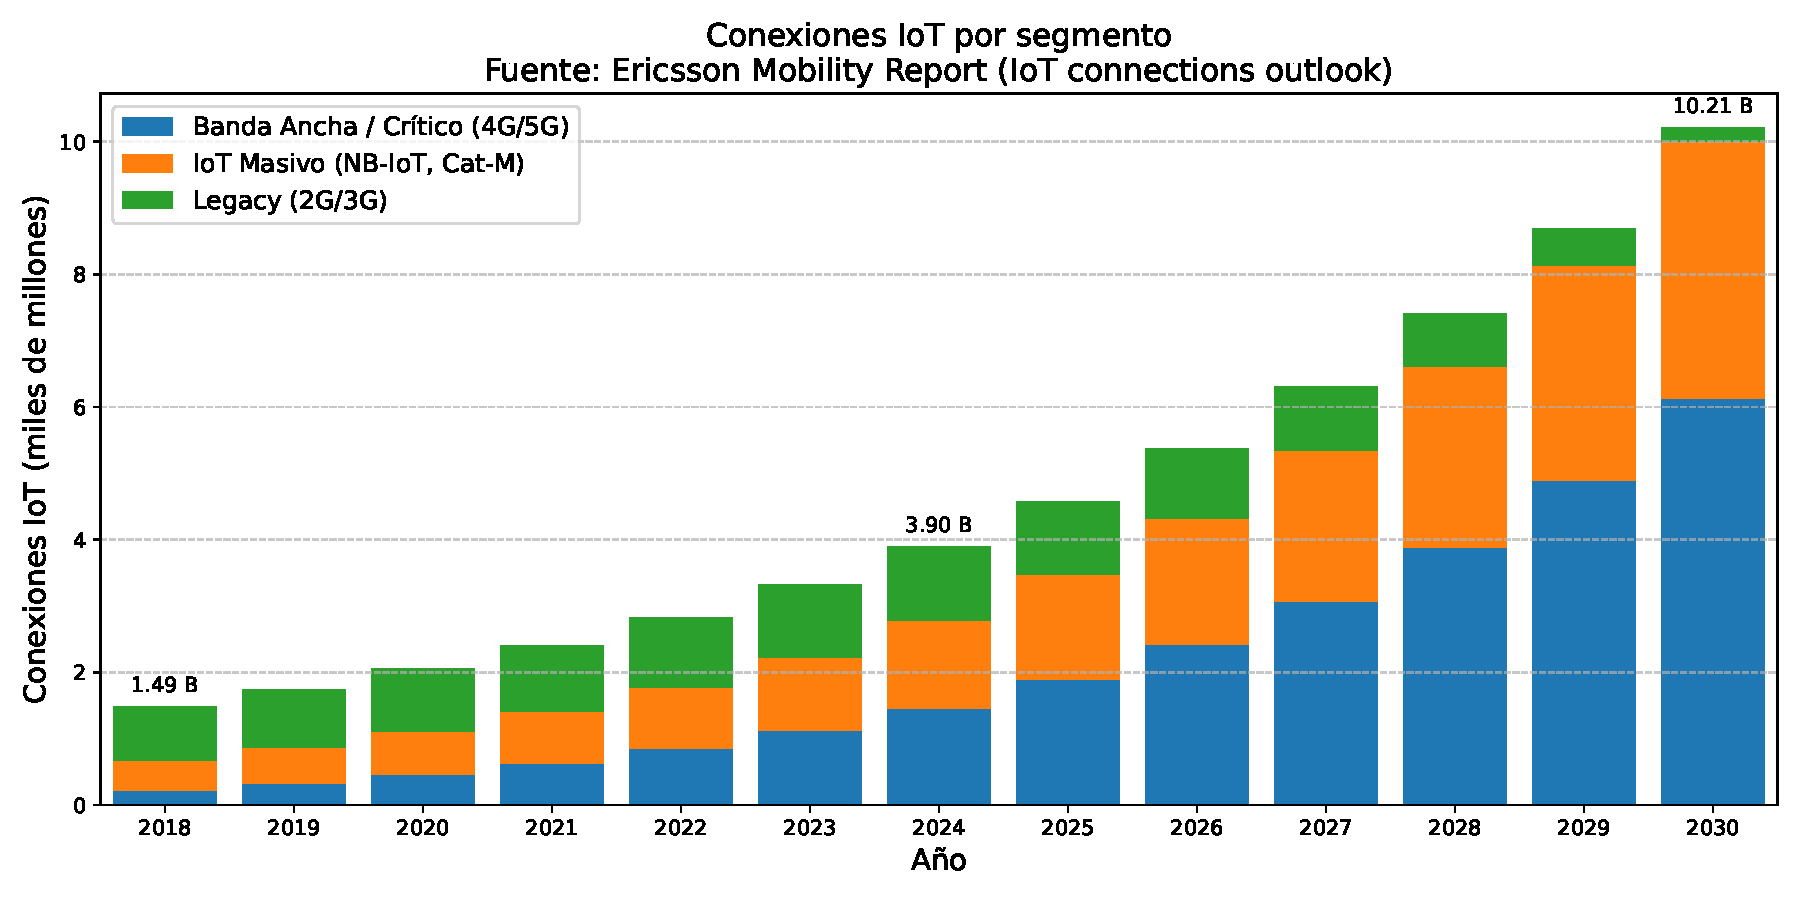
\includegraphics[width=\textwidth]{fig/04_in-band/in_band_1.pdf}
    \caption{Estudio del crecimiento de las conexiones de dispositivos IoT desglosadas por segmento~\cite{ericsson2025_iot}.}
    \label{fig:in_band_1}
\end{figure}


Un aspecto esencial de la nueva generación de redes móviles es la arquitectura de interconexión física que se propondrá. En \gls{5g}, la columna vertebral \gls{sdn} existente (en las redes móviles anteriores) se reutilizó incorporando modificaciones software para acomodar las nuevas especificaciones arquitectónicas mediante flexibilidad y programabilidad~\cite{Li2018}. En esta línea, cabe preguntarse si la futura red \gls{6g} aprovechará los beneficios de \gls{sdn} para el procesamiento de datos en su \textit{backbone}. Los informes preliminares sobre el diseño de \gls{6g}~\cite{uusitalo20216g,6garch1,6garch2} indican que \gls{sdn}, junto con tecnologías como \gls{p4} y técnicas de \gls{ai}/\gls{ml}, se emplearán para definir el plano de procesamiento de datos y mejorar el rendimiento y la orquestación de la infraestructura existente. Además, las redes \gls{6g} enfatizarán la necesidad del paradigma \gls{mec}, extendiendo el borde de la red hacia los usuarios y construyendo el llamado continuo \textit{edge-to-cloud} (o simplemente \textit{cloud continuum})~\cite{Milojicic20}. Aunque \gls{sdn} sigue siendo un pilar del \textit{edge computing}, existen aún desafíos en la integración de \gls{iot} y \gls{sdn} en el borde de la red~\cite{Bittencourt18}, tales como la adaptación de estándares y recomendaciones \gls{sdn} a entornos inalámbricos, y la compatibilidad con dispositivos heterogéneos y con recursos restringidos, característicos de las redes \gls{iot} (Según se ha analizado en el Capítulo~\ref{ch:problema}).\\
\\
En el caso específico del plano de control \gls{sdn}, se consideran dos paradigmas de control: \textit{out-of-band} e \textit{in-band} (Según se estudió en la Sección~\ref{subsec:arquitectura_fisica_sdn}). Mientras que en el enfoque \textit{out-of-band} cada nodo \gls{sdn} dispone de un enlace dedicado al controlador (es decir, la información de control circula por una red dedicada), en el modelo \textit{in-band} sólo ciertos nodos gestionados cuentan con enlace directo al controlador y el resto de dispositivos reutilizan dichos enlaces para reenviar la información de control hacia el controlador \gls{sdn} (la información de control, al no disponer de una red dedicada, viaja conjuntamente con el tráfico de datos hasta alcanzar el controlador). Aunque no existe un paradigma de control intrínsecamente superior, cada enfoque tiene ventajas e inconvenientes y la elección depende del caso de uso concreto, los dispositivos \gls{iot} con recursos restringidos en el extremo de la red se benefician en general del control \textit{in-band}: aunque potencialmente menos seguro~\cite{feghali2015sdn}, sus requisitos computacionales y energéticos suelen ser inferiores. No obstante, según se revisó (Sección~\ref{subsec:conclu_inband}), no existe un estándar específico que defina el control \textit{in-band}; y, si bien existen propuestas en la literatura, pocas contemplan entornos inalámbricos y ninguna está diseñada explícitamente para dispositivos con recursos limitados.\\
\\
En este capítulo se presenta, \texttt{win-BOFUSS}, una solución evolucionada del switch \gls{bofuss} que soporta control \textit{in-band} para escenarios inalámbricos, diseñada de forma escalable y orientada a dispositivos \gls{iot}.

\section{Descripción del protocolo}
\label{sec:inband_proto_desc}
El Estado del Arte ha puesto de manifiesto que el etiquetado jerárquico y las técnicas basadas en árboles enraizados constituyen un marco fértil y consolidado para abordar el arranque y la provisión de canales de control en entornos densos y heterogéneos (Ver Sección~\ref{subsubsec:conclu_etiquetado}). Las propuestas revisadas comparten la idea de explotar información codificada localmente en etiquetas para reducir estado y facilitar encaminamiento hacia la raíz o raíces. Es por ello, que nuestro protocolo \textit{in-band} busca y establece múltiples rutas entre un nodo raíz y el resto de los nodos de la topología, creando múltiples árboles conectados. La novedad de este protocolo es que permite al controlador \gls{sdn} comunicarse mediante canales \textit{in-band} en entornos inalámbricos, lo cual no es común dado que \gls{sdn} fue diseñado originalmente para escenarios cableados. 
Existen propuestas enfocadas de etiquetado jerárquico en redes \gls{llns} (IoTorii, de Rojas \textit{et al.}~\cite{rojas2021outperforming}), que al igual que esta solución, están concebidas para requerir pocos recursos computacionales y de memoria en dispositivos restringidos, sin embargo, esta propuesta habilita a los nodos \gls{iot} interactuar de forma nativa en entornos \gls{sdn}. Por lo tanto, resulta particularmente adecuado para redes \gls{iot}-\gls{sdn}. Asimismo, gracias a la funcionalidad \textit{multipath} que ofrece el protocolo, también es posible almacenar diferentes rutas de respaldo que pueden utilizarse en caso de fallos o en escenarios de movilidad dentro del área de cobertura, manteniendo siempre activa la sesión con el controlador.\\
\\
La definición de este protocolo se apoya en el trabajo de Constantin \textit{et al.}~\cite{constantin2020desarrollo}, en el que se establecen múltiples rutas entre un nodo raíz y el resto de nodos de la topología en un escenario cableado. Estas múltiples rutas se construyen combinando dos técnicas (según se explicaba en la Sección~\ref{subsubsec:teminologia_grafos}): el etiquetado jerárquico de los dispositivos y una inundación controlada de dichas etiquetas. En primer lugar, se selecciona un nodo raíz de la red (generalmente un nodo con acceso al controlador \gls{sdn}), y dicho nodo genera un mensaje inicial con una etiqueta específica que envía a sus nodos directamente conectados. El dispositivo receptor inunda este mensaje a sus vecinos a través de todas las interfaces excepto aquella por la que recibió el mensaje. Además, añade un nuevo elemento a la etiqueta recibida por cada interfaz de salida con el fin de rastrear la ruta recorrida a lo largo de la topología. Cada vecino que recibe el mensaje repetirá este proceso. El proceso de inundación puede detenerse en cualquier nodo considerando parámetros específicos de la etiqueta recibida, tales como la longitud de la etiqueta, el prefijo común de la etiqueta, entre otros. Eventualmente, cada nodo recibirá un conjunto de etiquetas jerárquicas que identifican múltiples rutas para alcanzar el nodo raíz (quien envió la primera etiqueta) desde el nodo actual. Si el nodo raíz es un nodo conectado al controlador \gls{sdn}, entonces cada nodo podrá establecer comunicación con el controlador a través de cualquiera de esas rutas etiquetadas. Estas etiquetas reciben el nombre de \gls{hlmac}, siguiendo la idea del estándar IEEE 802c-2017~\cite{ieee802c2017}, que define el uso de direcciones \gls{mac} locales. \\
\\
Nuestro protocolo adapta la idea original a entornos inalámbricos. El reto principal en estos escenarios es que, a diferencia de las redes cableadas, los dispositivos inalámbricos suelen disponer de una única interfaz radio que les permite comunicarse con todos los vecinos dentro de su área de cobertura; por tanto, el mecanismo de etiquetado jerárquico propuesto en~\cite{constantin2020desarrollo} no puede aplicarse directamente. Para solventar esta limitación incorporamos conceptos tomados de IoTorii de Rojas \textit{et al.}~\cite{rojas2021outperforming} (una línea de trabajo en la que participé antes del Doctorado) y adaptamos el etiquetado a la naturaleza broadcast del medio inalámbrico. Concretamente, el proceso se basa en identificar previamente los vecinos que se encuentran realmente en rango de cobertura y, sobre esa información local, asignar las etiquetas jerárquicas correspondientes en función de la relación de vecindad (y no del puerto de salida). De este modo cada nodo construye su vista local del entorno y puede generar/propagar etiquetas coherentes para el encaminamiento en topologías inalámbricas. \\
\\
Por tanto, el protocolo se basa en dos procesos fundamentales que operan de forma complementaria:

\begin{itemize}

\item \textbf{Reconocimiento de vecindad} (Detallado en la sub-Sección~\ref{subsubsec:procesoVecinos}): Mecanismo local y periódico mediante el cual cada nodo detecta y mantiene la lista actualizada de vecinos en rango (tabla de vecinos). Esta información sirve para identificar enlaces activos, eliminar vecinos “muertos” y proporcionar la base para la asignación de identificadores locales que sustituyen al concepto de puerto físico en entornos cableados.

\item \textbf{Etiquetado jerárquico} (Detallado en la sub-Sección~\ref{subsubsec:procesoEtiquetado}): Proceso de generación y difusión controlada de etiquetas (\gls{hlmac}) que permite construir uno o varios árboles enraizados en los nodos con acceso al controlador \gls{sdn}. El etiquetado utiliza la información de vecindad para propagar rutas jerarquizadas, reducir el estado por nodo y habilitar encaminamiento multipath y protección ante fallos o movilidad.

\end{itemize}

\subsection{Proceso de reconocimiento de vecindad}
\label{subsubsec:procesoVecinos}

El proceso de reconocimiento de vecindad es un proceso ligero y periódico cuya función es mantener, en cada nodo, una tabla de vecinos con entradas de tipo tuplas, donde se asocia cada dirección \gls{mac} vecina con un identificador local (ID). Esta tabla se actualiza  localmente en cada nodo mediante mensajes \textit{Hello}, que cada nodo difunde periódicamente en su área de cobertura. Por tanto, los objetivos del proceso de reconocimiento de vecindad son los siguientes:

\begin{itemize}
    \item Detectar vecinos nuevos. Al recibir un mensaje \textit{Hello}, el nodo inspecciona la dirección \gls{mac} remitente; si no está presente en la tabla de vecinos, se crea una nueva entrada almacenando la asociación \((MAC \rightarrow ID)\). La ID puede generarse como un contador incremental (sufijo) o mediante otro esquema determinista según la implementación.
    
    \item Detectar vecinos ``muertos''. Cada entrada en la tabla incorpora un temporizador (\textit{timeout}) que se refresca al recibir \textit{Hello} periódicos del vecino correspondiente. Si el temporizador expira, la entrada se elimina y se invalidan las rutas que dependieran de dicho vecino, asumiendo una ausencia por fallo o movilidad.
    
    \item Parametrización y control de señalización. El periodo de emisión de mensajes tipo \textit{Hello} y los umbrales de \textit{timeout} son parámetros configurables que permiten adaptar el coste de señalización a la densidad y movilidad del despliegue (p. ej., intervalos más largos en redes muy densas o donde la energía es limitada).
    
    \item Escalabilidad local. El mecanismo está diseñado para que la carga por nodo dependa principalmente de su grado de conectividad (número de vecinos). Esto facilita dimensionar recursos (memoria, CPU) y ajustar parámetros en dispositivos con capacidades limitadas.
\end{itemize}



Desde el punto de vista de coste, el mecanismo es muy simple: por cada ronda de descubrimiento, cada nodo emite un \textit{Hello} y recibe tantos \textit{Hello} como grado local de conectividad tenga. Esta caracterización ayuda a dimensionar el periodo de \textit{Hello} y el tiempo de expiración (\textit{timeout}) en función de la densidad y movilidad del despliegue.\\
\\
Para ilustrar este proceso, se presenta la Figura~\ref{fig:in_band_2}. Según se puede apreciar en el inferior de la Figura, se ha ejemplificado una topología inalámbrica de ejemplo, donde los enlaces representados indican que ambos nodos se encuentran en radio de cobertura. Tomando la Figura~\ref{fig:in_band_2} como ejemplo, podemos observar cómo se rellenarían las tablas de vecinos una vez el proceso hubiera convergido. En el caso del nodo \textit{A}, sólo detecta al nodo \textit{B} y almacenará la entrada \((\text{MAC}_B,\; \text{ID}=1)\). El nodo \textit{B} detecta a \(\{A,C,D\}\) y asigna tres IDs locales \(\{1,2,3\}\) respectivamente; \textit{C} registra a \(\{B,F\}\) con dos IDs, y así de forma análoga. Nodos con alta conectividad (p. ej. \textit{B} o \textit{D}) soportan mayor carga de recepción y mantienen más entradas, lo que debe tenerse en cuenta al dimensionar recursos en dispositivos con capacidades limitadas.\\
\\
Es por ello que, el proceso de reconocimiento de vecindad, apoyado en los mensajes \textit{Hello} y la tabla de vecinos proporcionan una base local, eficiente y fácilmente parametrizable para habilitar el etiquetado jerárquico y la construcción de árboles en entornos inalámbricos y móviles, controlando explícitamente el intercambio de señalización en función de la densidad y la movilidad de la red.

\begin{figure}[ht!]
    \centering
    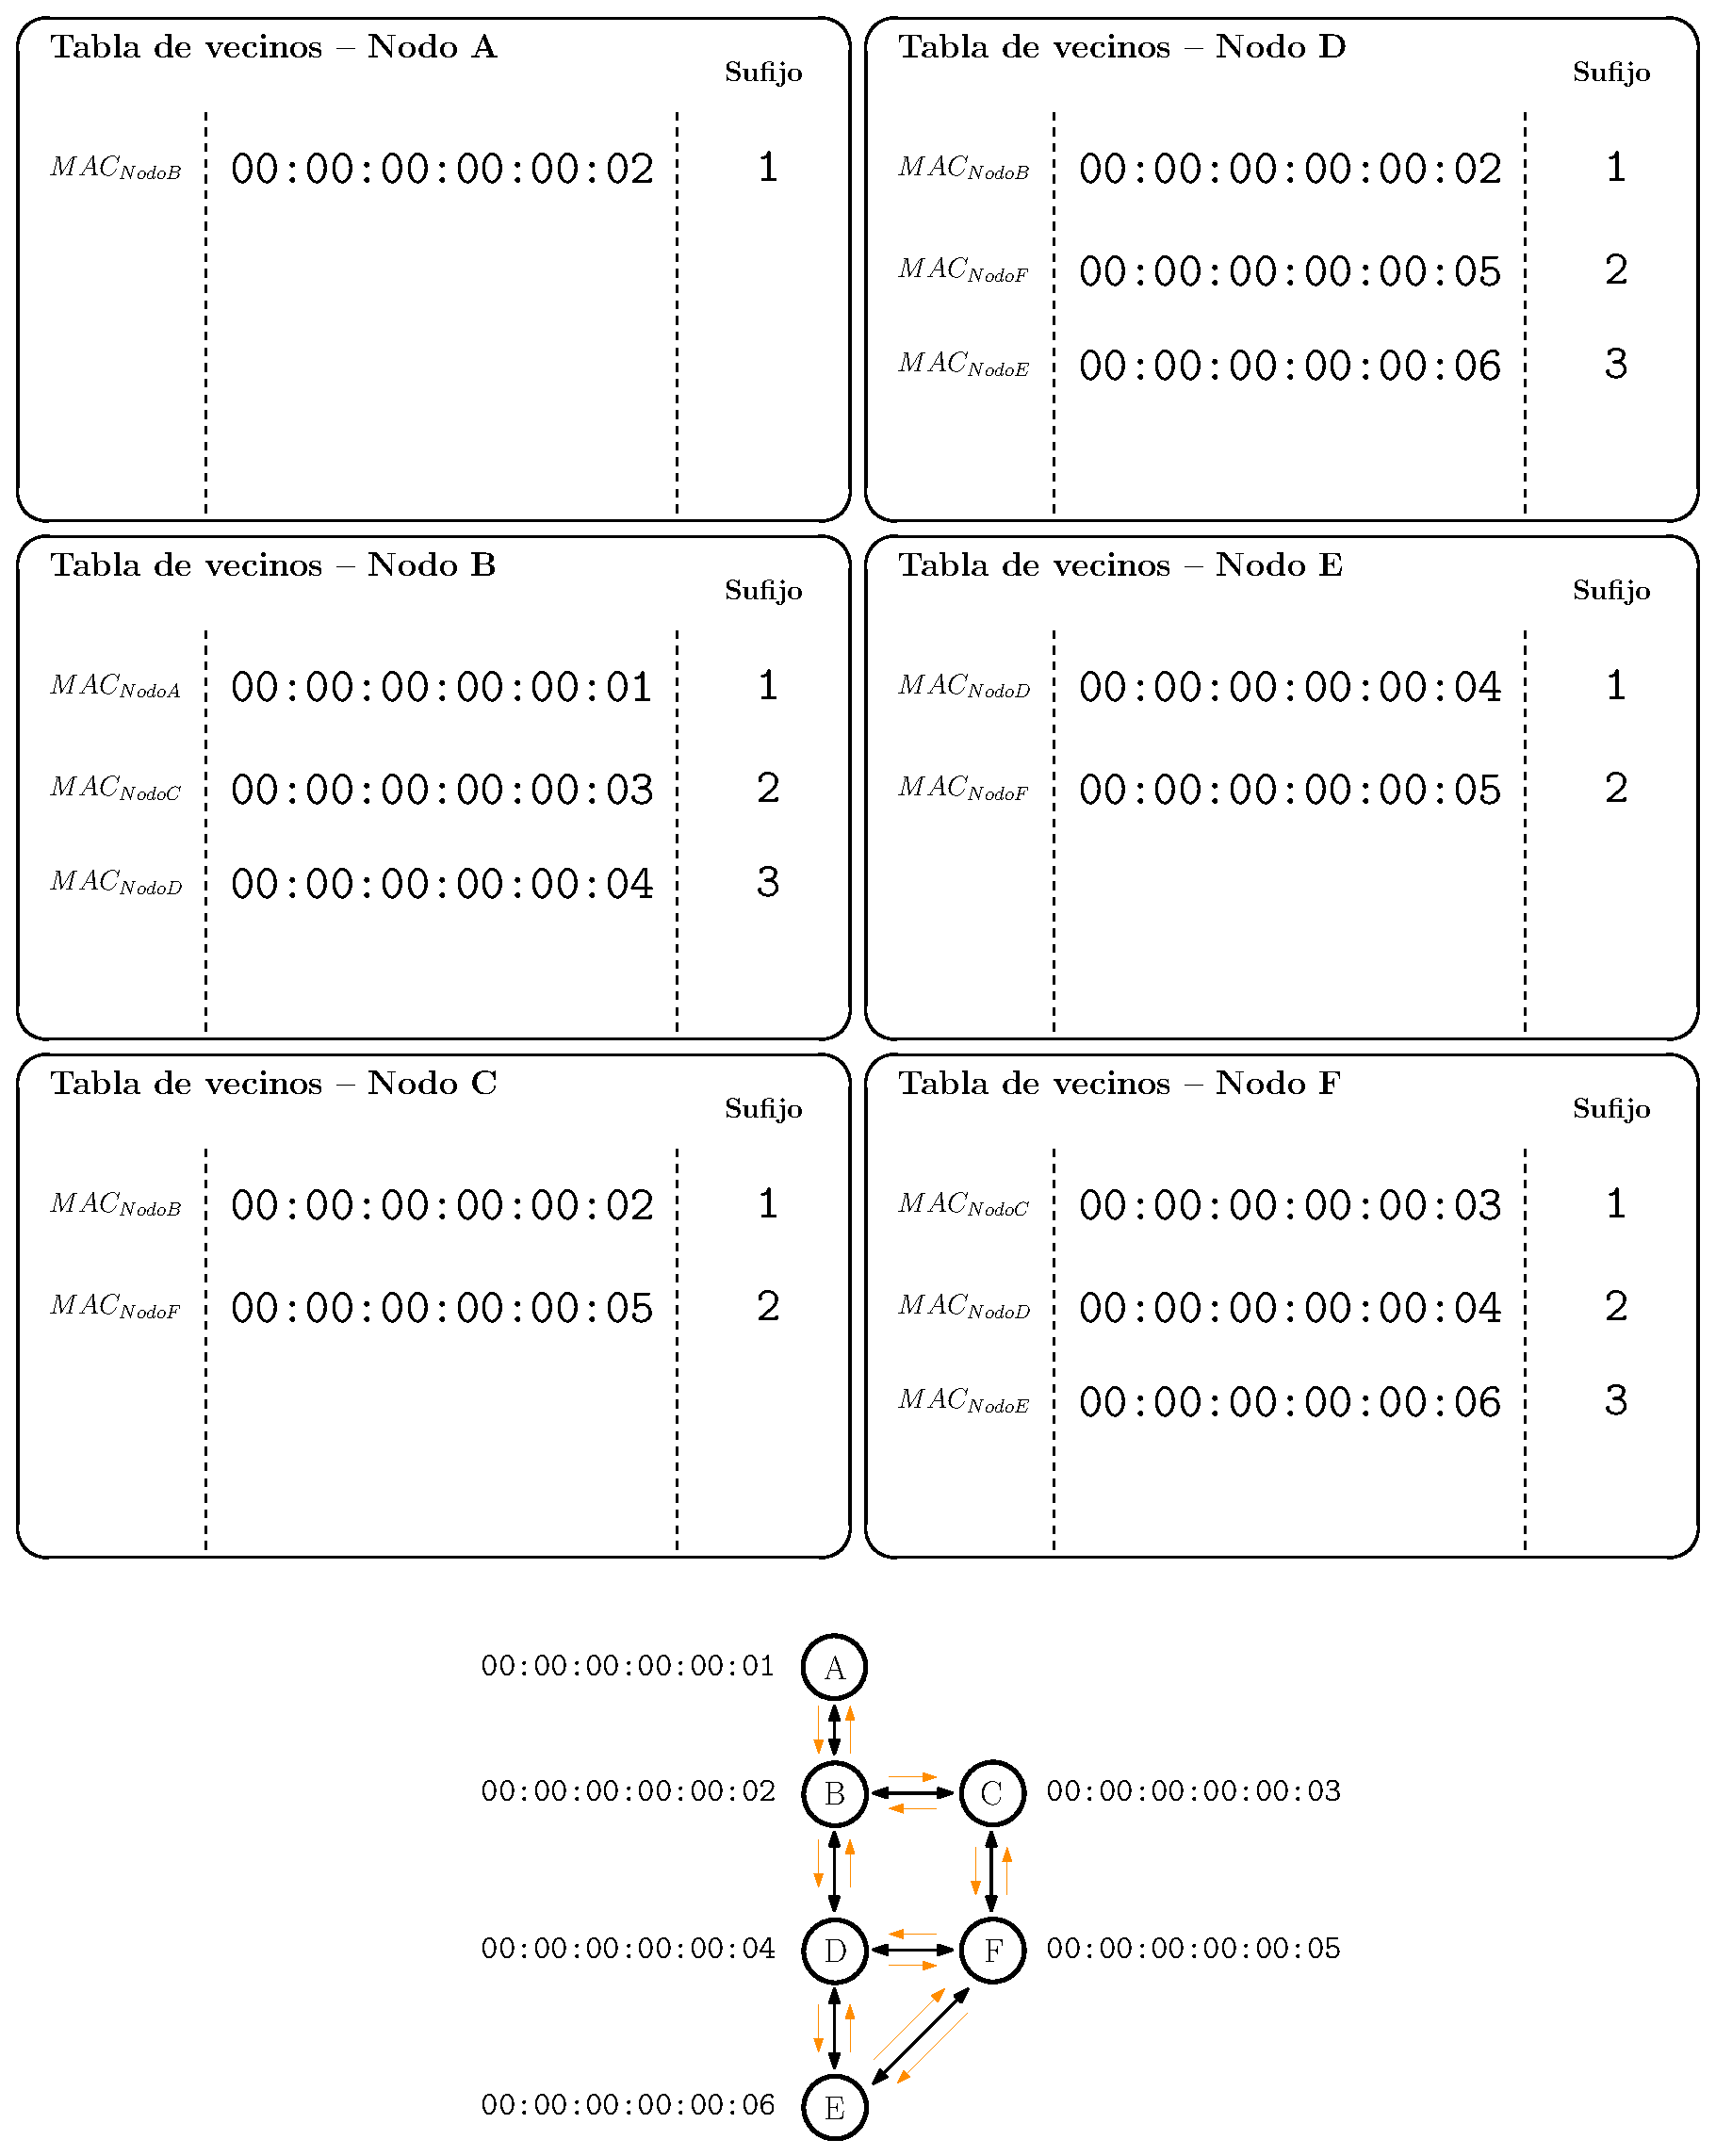
\includegraphics[width=\textwidth]{fig/04_in-band/in_band_2.eps}
    \caption{Proceso de reconocimiento de vecindad empleando las tablas locales de vecinos.}
    \label{fig:in_band_2}
\end{figure}

\subsection{Proceso de etiquetado jerárquico}
\label{subsubsec:procesoEtiquetado}

Una vez se ha explicado el proceso de reconocimiento de vecindad en la topología inalámbrica, se va a detallar el proceso de etiquetado jerárquico del protocolo. Para ilustrar y aclarar el proceso de construcción de la topología lógica a partir de la topología física, la Figura~\ref{fig:in_band_3} muestra el proceso de inundación de las \gls{hlmac} en una topología de ejemplo de seis nodos, donde el nodo \textit{A} actúa como nodo raíz (el que tendrá acceso con el controlador \gls{sdn}). El procedimiento arranca después de haberse intercambiado al menos una ronda de paquetes \textit{Hello}, es decir, cuando todos los nodos conocen a sus vecinos y han poblado sus tablas locales de vecinos con la asociación dirección \((MAC \rightarrow ID)\). Las áreas de cobertura y las relaciones de vecindad se representan con una flecha doble negra (por ejemplo, \textit{B} tiene por vecinos a \textit{A}, \textit{C} y \textit{D}). La figura se divide en cuatro subfiguras que representan pasos sucesivos del procedimiento.\\
\\
La Fig.~\ref{fig:in_band_3}(a) ilustra el primer paso del proceso: el nodo \textit{A} envía la primer \gls{hlmac}, que es recibida por el nodo \textit{B}. La \gls{hlmac} inicial enviada por \textit{A} está compuesta por el ID de \textit{A} y por el ID local que \textit{A} asignó a \textit{B}, representado como \textit{1.1}. Concretamente, \textit{A} sabe por el intercambio previo de los mensajes \textit{Hello} que sólo tiene un vecino (\textit{B}) y le asigna el ID \textit{1}. Cuando \textit{B} recibe \textit{1.1}, consulta su tabla local de vecinos y comprueba que tiene tres vecinos [\textit{A,C,D}] con ID locales [\textit{1,2,3}]. En ese contexto, \textit{A} se considera el nodo padre (que fue quien envió el \gls{hlmac} inicial) y \textit{C}, \textit{D} son nodos hijos. A continuación, \textit{B} genera dos nuevas \gls{hlmac}, \textit{1.1.2} y \textit{1.1.3}, y las envía a \textit{C} y \textit{D}, respectivamente; pero no se envía \gls{hlmac} al nodo padre. Es importante subrayar que no se inundan todos los nodos con \gls{hlmac} para evitar bucles: sólo se retransmiten aquellas \gls{hlmac} que no sean extendidas de una \gls{hlmac} previamente almacenada como hija. Por ejemplo, si \textit{B} ya ha guardado \textit{1.1} y en una iteración posterior recibe una \gls{hlmac} del tipo \textit{1.1.x...}, la descartará inmediatamente porque proviene de uno de sus hijos y por tanto representaría un bucle.\\
\\
La Fig.~\ref{fig:in_band_3}(b) muestra el segundo paso: las \glspl{hlmac} enviadas por \textit{B} (\textit{1.1.2} y \textit{1.1.3}) son recibidos por los nodos \textit{C} y \textit{D}. El nodo \textit{C} verifica que tiene dos vecinos [\textit{B,F}] con IDs [\textit{1,2}] y, por tanto, sólo genera y reenvía la \gls{hlmac} \textit{1.1.2.2} hacia su hijo \textit{F}. En el caso del nodo \textit{D}, con vecinos [\textit{B,F,E}] e IDs [\textit{1,2,3}] (donde \textit{F} y \textit{E} son hijos), produce \textit{1.1.3.2} y \textit{1.1.3.3} y las reenvía a \textit{E} y \textit{F}. El proceso se repite en \textit{E} y \textit{F}, tal y como se muestra en la Fig.~\ref{fig:in_band_3}(c), donde las nuevas \glspl{hlmac} aprendidas por cada nodo se resaltan en negrita. La subfigura inferior derecha (Fig.~\ref{fig:in_band_3}(d)) recoge el conjunto final de \glspl{hlmac} almacenadas en todos los nodos de la topología.\\
\\
Al finalizar el procedimiento, cada nodo habrá almacenado múltiples \glspl{hlmac}, es decir, varias rutas posibles hacia la raíz. Por ejemplo, \textit{B} sólo tendrá un \gls{hlmac} (una única ruta hacia la raíz), mientras que \textit{C}, \textit{D} y \textit{F} dispondrán de tres \glspl{hlmac} (tres rutas hacia el nodo raíz) y \textit{E} de cuatro \glspl{hlmac}, teniendo más opciones para alcanzar al nodo que da acceso al controlador \gls{sdn}. Además, el número total de \glspl{hlmac} por nodo puede limitarse a un valor prefijado, de modo que cada nodo mantenga como máximo un número de rutas, lo que representa una tensión entre cantidad de información de estado por nodo contra la capacidad de resiliencia con rutas de respaldo a nivel de nodo. 

\begin{figure}[ht!]
     \centering
     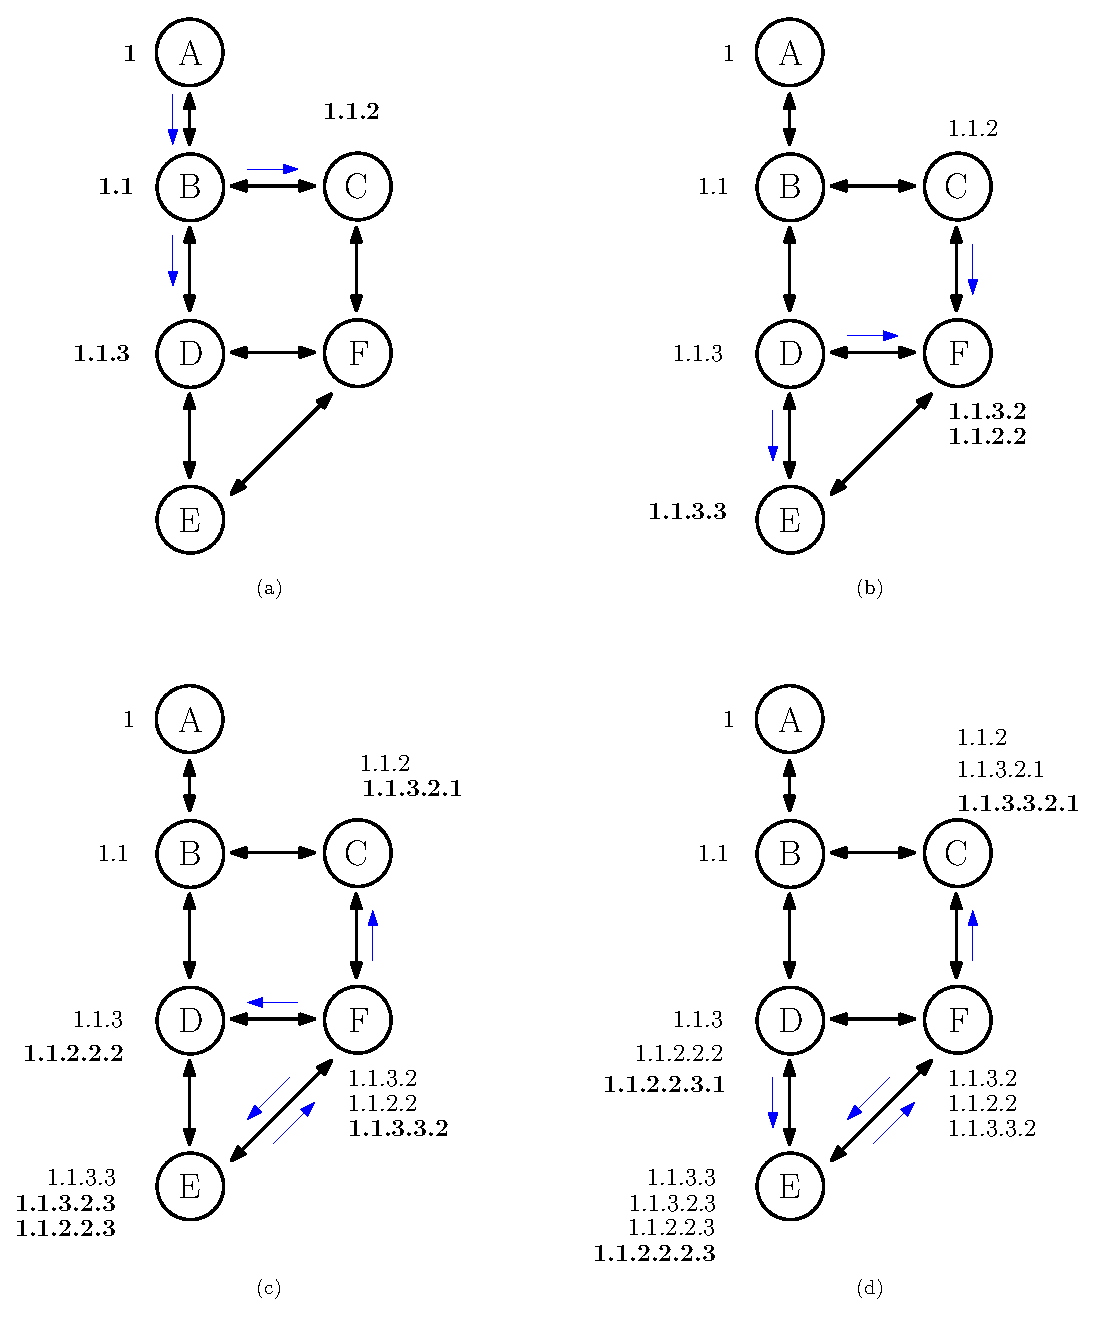
\includegraphics[width=\textwidth]{fig/04_in-band/in_band_3.eps}
     \caption{Proceso de difusión de etiquetas Hierarchical Local MAC (HLMAC) en la topología de ejemplo.}
     \label{fig:in_band_3}
\end{figure}

La elección de que ruta utilizar depende de criterios del caso de uso final, y de las características propias de la topología, pudiendo optar por el menor número de saltos, menor latencia, máxima redundancia, entre otros. En este caso, al ser una prueba de concepto, no se ha explorado en profundidad el impacto de los criterios, y se ha aplicado la elección de la \gls{hlmac} con menor latencia, obteniendo la siguiente topología lógica según se indica en la Figura~\ref{fig:in_band_4}. Si consideramos todas las $HLMAC_{active}$ de los nodos en la topología, podemos definir una topología lógica que contiene todos los nodos de la topología física pero solo un subconjunto de los enlaces presentes en dicha topología física. La formulación del proceso de establecimiento la topología lógica se puede encontrar descrito en la Sección~\ref{subsubsec:teminologia_grafos}. Es importante resaltar que este proceso de selección de rutas y asignación de \gls{hlmac} tiene un impacto significativo en la eficiencia y utilización de los enlaces en la topología. Aquellos enlaces que no sean utilizados, quedan en desuso, lo que podría liberar recursos y mejorar la capacidad de la red para adaptarse a cambios en la topología.


\begin{figure}[ht!]
     \centering
     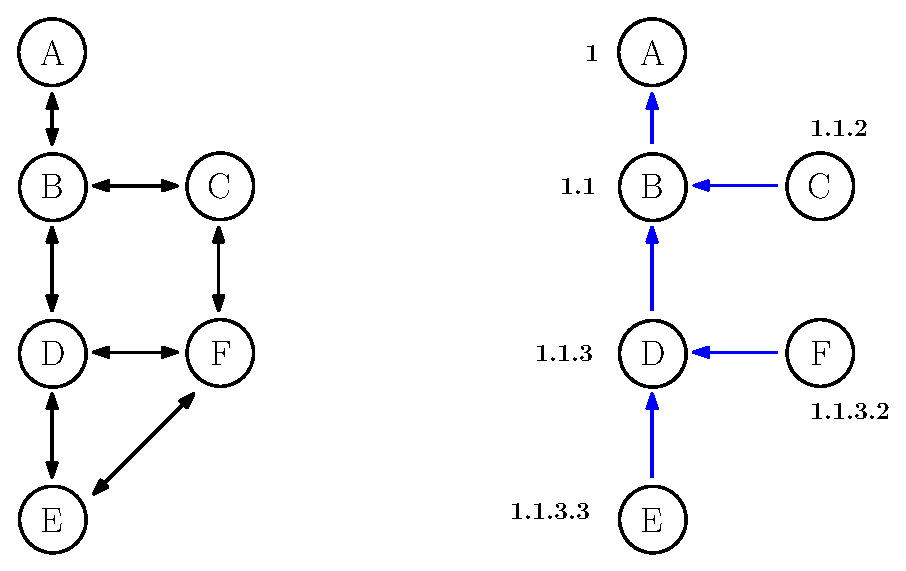
\includegraphics[width=0.7\textwidth]{fig/04_in-band/in_band_4.eps}
     \caption{Establecimiento de la topología lógica.}
     \label{fig:in_band_4}
\end{figure}


La principal ventaja de este diseño \textit{in-band} es su simplicidad, en el caso más sencillo, el protocolo puede operar con una única \gls{hlmac} asignada por nodo, es decir,  una sola entrada de enrutamiento, y, aun así, ofrecer conectividad con el controlador. Además, el número de \glspl{hlmac} que requiere cada dispositivo es independiente del tamaño total de la red, además de configurable, lo que reduce drásticamente la memoria necesaria en dispositivos \gls{iot} con recursos limitados. \\
\\
En cuanto al número de mensajes intercambiados, cada nodo sólo necesita enviar un mensaje \textit{Hello} periódico y tantas transmisiones de asignación de \glspl{hlmac} como caminos \textit{multipath} se configuren; si sólo se mantiene una \gls{hlmac}, bastan únicamente dos mensajes periódicos en total. Estos intercambios están basados en eventos, y su dinámica es comparable a la difusión de un mensaje desde el nodo raíz hacia el resto de la red, proceso que suele ser rápido en comparación con protocolos de estado de enlace. Por último, la frecuencia de estas actualizaciones es configurable en función de la movilidad: escenarios con alta movilidad requieren periodos cortos, mientras que entornos estáticos pueden emplear periodos más largos.

\section{Implementación de wireless In-Band Basic OpenFlow Software Switch (win-BOFUSS)}

La implementación del protocolo se ha realizado sobre la plataforma \textit{Basic OpenFlow Software Switch} (\gls{bofuss}). Esta elección no ha sido arbitraria, ya que, en comparación con otros software-switches ampliamente utilizados, como \gls{ovs}, \gls{bofuss} ofrece un datapath cuya implementación resulta más sencilla de desarrollar y depurar, al ejecutarse en espacio de usuario y no en espacio de \textit{kernel}.\\
\\
Los orígenes de \gls{bofuss} se remontan a 2008, cuando en la Universidad de Stanford se desarrolló la primera implementación de referencia del protocolo OpenFlow, denominada \textit{The Stanford Reference OpenFlow Switch} (McKeown \textit{et al.}~\cite{mckeown2008openflow}). Dicho desarrollo constituyó un producto mínimo viable, concebido con el objetivo de demostrar el funcionamiento del protocolo y facilitar el proceso de estandarización de OpenFlow 1.0. Posteriormente, el proyecto fue retomado por los laboratorios de Ericsson, donde se amplió su funcionalidad para soportar OpenFlow 1.1 (Lajos \textit{et al.}~\cite{of11softswitch}). Años más tarde, el trabajo fue continuado por el investigador Eder Fernandes en el marco de su TFM y su tesis doctoral en Brasil~\cite{fernandes2014openflow}, consolidando lo que actualmente conocemos como \gls{bofuss}, con soporte para OpenFlow 1.3 (Fernandes \textit{et al.}~\cite{fernandes2020road}). Posteriormente, este software switch fue extendido por mi compañero de laboratorio, Constantin, quien implementó capacidades de comunicación \textit{in-band} en entornos cableados (Constantin \textit{et al.}~\cite{constantin2020desarrollo}). A partir de esta última versión, y teniendo en cuenta las lecciones aprendidas de IoTorii (Rojas \textit{et al.}~\cite{rojas2021outperforming}), se desarrolló \texttt{win-BOFUSS}, una implementación del software switch con soporte \textit{in-band} en redes inalámbricas de baja capacidad. En la Figura~\ref{fig:in_band_5} se muestra la evolución histórica del desarrollo del switch, desde su origen en 2008 con la propuesta del protocolo OpenFlow, hasta la actual implementación de \texttt{win-BOFUSS} (Carrascal \textit{et al.}~\cite{carrascal2023scalable}).

\begin{figure}[ht!]
    \centering
    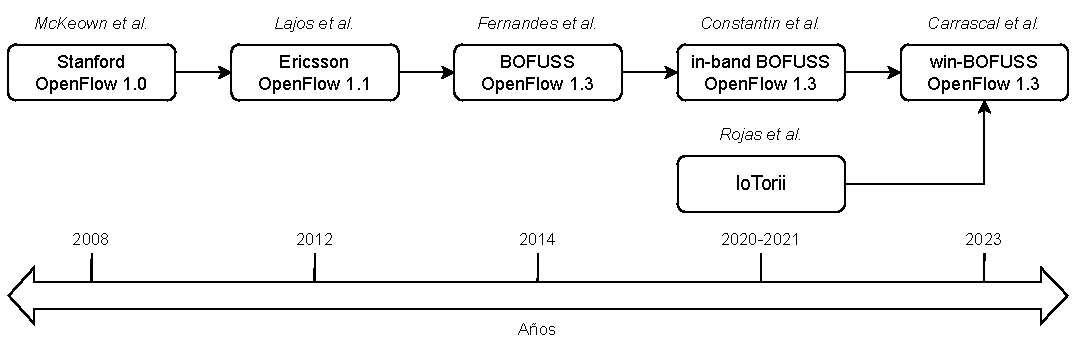
\includegraphics[width=\textwidth]{fig/04_in-band/in_band_5.drawio.pdf}
    \caption{Evolución cronológica del desarrollo del software switch BOFUSS.} 
    \label{fig:in_band_5}
\end{figure}

En la Figura~\ref{fig:in_band_6} se muestra el diagrama de flujo que recoge la implementación de la lógica del protocolo. Por defecto, \gls{bofuss} no arranca con la funcionalidad \emph{in-band} habilitada, por lo que al invocar el proceso en espacio de usuario, donde, entre otras cosas, se especifican las interfaces a gestionar, es preciso activar explícitamente la lógica \emph{in-band} mediante el parámetro \texttt{--inband}. Tras la inicialización del protocolo, el primer paso consiste en configurar los temporizadores: los asociados al envío periódico de mensajes \textit{Hello} y los vinculados a las entradas de las tablas de vecinos y de \gls{hlmac}. A continuación, cada nodo utiliza su interfaz inalámbrica para emitir el primer mensaje \textit{Hello} y así descubrir qué dispositivos se encuentran dentro de su área de cobertura, estableciendo, de ese modo, las relaciones de vecindad iniciales. Completada la fase de inicialización, el sistema entra en el bucle principal de la lógica del protocolo, que gestiona el refresco de temporizadores, la recepción y procesamiento de \textit{Hello}s y \gls{hlmac}s, y las acciones de mantenimiento de tablas y rutas.

\begin{figure}[ht!]
    \centering
    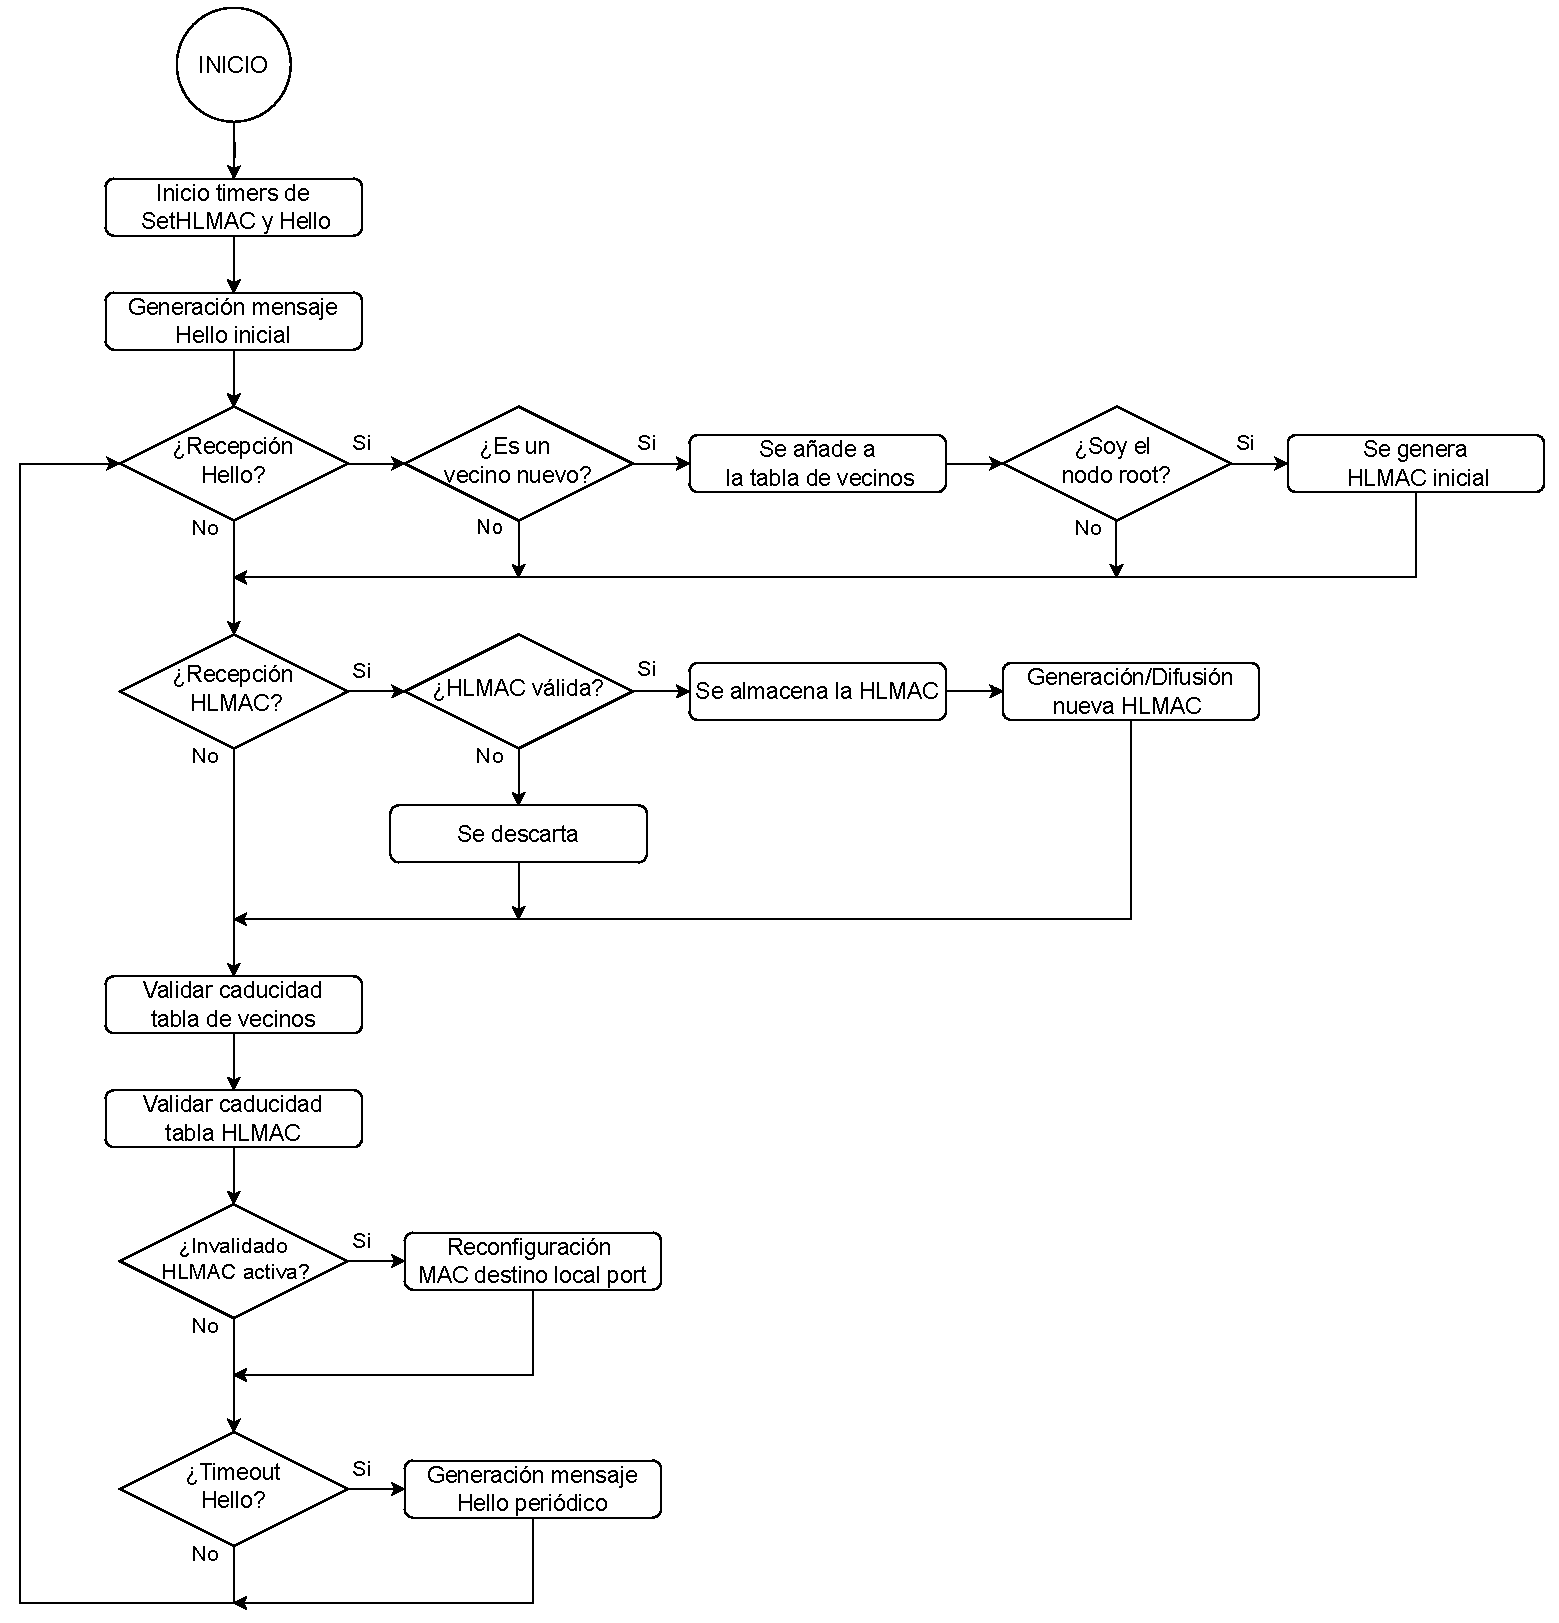
\includegraphics[width=\textwidth]{fig/04_in-band/in_band_6.drawio.pdf}
    \caption{Diagrama de flujo de la implementación sobre el software switch BOFUSS.} 
    \label{fig:in_band_6}
\end{figure}

En el bucle principal se gestionan de forma \textit{event-driven} los siguientes sucesos: recepción de un mensaje \textit{Hello}, recepción de una \gls{hlmac}, expiración de entradas en la tabla de vecinos, expiración de entradas en la tabla de \gls{hlmac}, verificación de la ruta principal (posible reconfiguración) y vencimiento del temporizador periódico de envío de \textit{Hello}. Al recibir un \textit{Hello} se comprueba si el emisor es un vecino nuevo; en ese caso se inserta la entrada correspondiente en la tabla de vecinos y se inicia su temporizador. Si el emisor es el nodo raíz (\textit{root}), además se genera el \gls{hlmac} inicial que pone en marcha la asignación jerárquica de etiquetas en la topología. Al recibir una \gls{hlmac}, se valida que no represente un bucle; si es válida se almacena en la tabla de \gls{hlmac} y, acorde con el procedimiento descrito en la Sección~\ref{subsubsec:procesoEtiquetado}, se difunde a los hijos correspondientes. Posteriormente, se evalúan los criterios para activar la dirección \gls{hlmac} preferente y se actualizan las rutas. Finalmente, en cada iteración se comprueba la caducidad de las entradas de las tablas (que se refrescan con la llegada de mensajes coincidentes) y se actúa en consecuencia: eliminar vecinos o \gls{hlmac} caducados, o forzar una reconfiguración si la ruta principal ha dejado de ser válida.\\
\\
Cuando una ruta almacenada en la tabla \gls{hlmac} deja de renovarse, es decir, el nodo correspondiente al siguiente salto deja de enviar mensajes \textit{Hello}, la entrada se invalida y el mecanismo elige la siguiente ruta disponible en la misma tabla. Dado que la interfaz física no cambia (misma interfaz inalámbrica), el puerto local permanece, pero sí varía el \textit{next-hop}: es necesario actualizar la dirección \gls{mac} de destino asociada a la IP del siguiente salto en la pila del sistema para que los paquetes salientes alcancen al nuevo vecino. En sistemas Linux esta actualización se puede realizar mediante Netlink, concretamente enviando un mensaje del tipo \texttt{RTM\_NEWNEIGH} para modificar la caché ARP. El procedimiento general es el siguiente: abrir un socket Netlink hacia el kernel, construir el mensaje \texttt{RTM\_NEWNEIGH} con los atributos adecuados (IP objetivo y nueva dirección \gls{mac} de enlace), enviarlo y gestionar la respuesta/confirmación del \textit{kernel}. Tras esta operación, los paquetes destinados a la IP en cuestión deberán resolverse hacia la nueva \gls{mac}. En la implementación actual se ha observado una limitación práctica: la actualización de la entrada ARP no siempre es suficiente para mantener transparente una conexión TCP ya establecida con el controlador, por lo que, como solución robusta y sencilla, el prototipo vuelve a establecer la sesión TCP tras actualizar la información de \textit{next-hop}. En trabajos futuros se explorará una integración más fina (p. ej. manipulación de tablas de encaminamiento/vecindad sin interrumpir sockets existentes o el uso de opciones de \textit{kernel} que permitan refrescar la resolución de enlace de forma totalmente transparente).\\
\\
Por último, se verifica el vencimiento del temporizador periódico de \textit{Hello}; si ha caducado, se emite un nuevo mensaje \textit{Hello} que refresca el estado en las tablas de los vecinos. La resiliencia del protocolo depende en gran medida de su capacidad para detectar y recuperarse con rapidez ante fallos y cambios topológicos. Ajustando adecuadamente el periodo de los \textit{Hello} y los tiempos de caducidad de las entradas, el protocolo puede identificar con rapidez enlaces caídos, nodos inalcanzables o la aparición de nuevos vecinos, reconstruir la tabla de vecinos y conmutar a rutas alternativas cuando proceda. Este mecanismo reduce el impacto de las interrupciones, acelera la convergencia de la red y optimiza el uso de los recursos disponibles.

\section{Evaluación}

El banco de pruebas elegido para llevar a cabo la prueba de concepto del protocolo es un entorno de emulación que utiliza, como biblioteca base, el software switch implementado, \texttt{win-BOFUSS}. No obstante, \gls{bofuss} no incorpora soporte inalámbrico nativo, por lo que se ha recurrido al módulo \texttt{mac80211\_hwsim} para emular el medio inalámbrico. En este escenario, cada instancia de \texttt{win-BOFUSS} combinada con \texttt{mac80211\_hwsim} actúa como un dispositivo inalámbrico \gls{iot} con una tarjeta Wi-Fi virtual, permitiendo emular escenarios inalámbricos en una única máquina física. La Figura~\ref{fig:in_band_7} ilustra la combinación de estas herramientas en una máquina. Como puede observarse, cada dispositivo \gls{iot} se emula encapsulándolo en una \textit{Network Namespace} para aislarlo (desde un punto de vista de red) del resto y forzar su comunicación mediante \texttt{mac80211\_hwsim}. Este módulo define los radios Wi-Fi de cada tarjeta virtual y solo intercambia información entre nodos que se encuentran dentro de su área de cobertura.\\
\\
Las características del medio radio (por ejemplo, limitaciones de transmisión por nodo) se configuran mediante el Traffic Controller (TC) de Linux. La información generada atraviesa las capas hasta llegar a la instancia de  \texttt{win-BOFUSS}, que implementa la lógica del protocolo propuesto. Las topologías de los escenarios se construyen mediante un conjunto de shell-scripts que definen el \textit{Network Namespace} aislado de cada dispositivo, su posición en un plano y su área de cobertura, de forma análoga a emuladores conocidos como Mininet o Mininet-WiFi~\cite{mininet-wifi}, lo que facilita la definición y despliegue de los escenarios y la integración con herramientas auxiliares (por ejemplo, trazado y representación de topologías).

\begin{figure}[ht!]
    \centering
    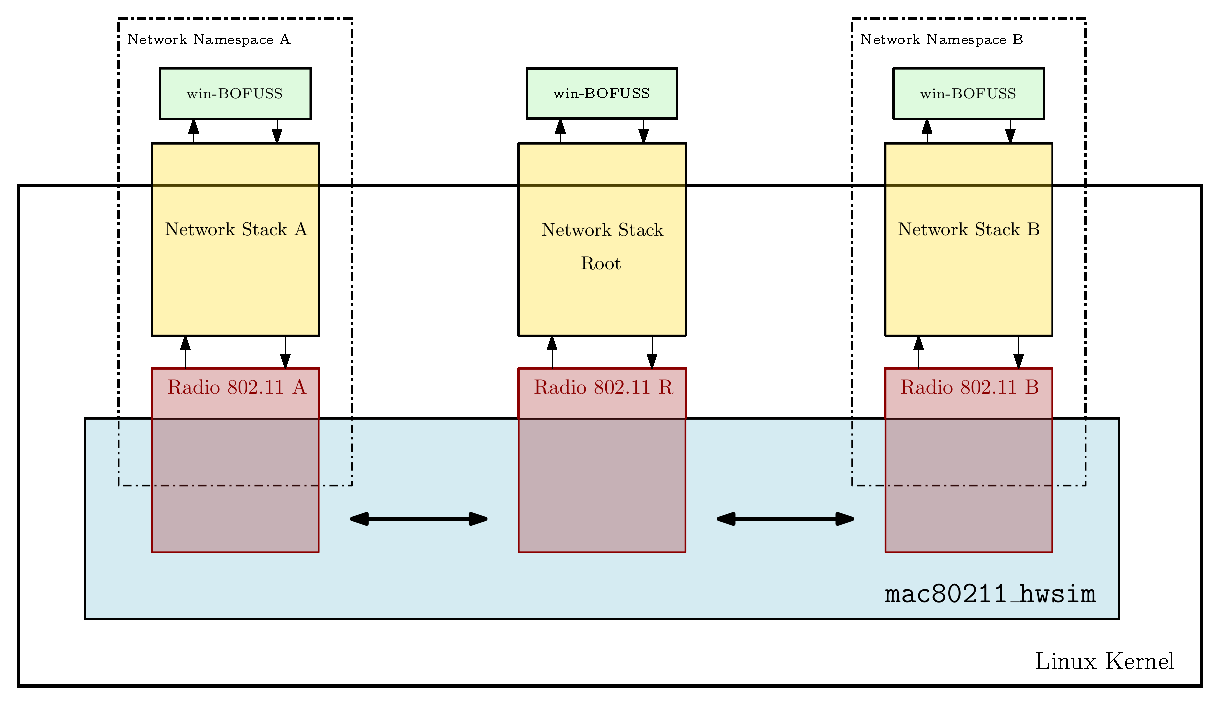
\includegraphics[width=0.95\textwidth]{fig/04_in-band/in_band_7.eps}
    \caption{Entorno de validación mediante emulación empleando el módulo del \textit{kernel} \texttt{mac80211\_hwsim}.} 
    \label{fig:in_band_7}
\end{figure}

Para la prueba de concepto de nuestro protocolo de control \gls{sdn} \textit{in-band}, denominado \texttt{win-BOFUSS}, se eligió la topología de la Figura~\ref{fig:in_band_3} con el fin de validar el comportamiento descrito en la Sección~\ref{sec:inband_proto_desc}. La Figura~\ref{fig:figuraCompleta} muestra dicha topología empleando las herramientas de visualización: a la izquierda el visualizador de grafos de Mininet-WiFi (Ver Figura~\ref{fig:subfiguraA}) y a la derecha el visor de topología del controlador Ryu (Ver Figura~\ref{fig:subfiguraB}). Para comprobar el funcionamiento \textit{in-band} de la propuesta, el controlador \gls{sdn} Ryu se lanza en la \textit{Network Namespace} raíz, en la cual solo se encontrará corriendo uno de los nodos de la topología, por lo que el resto tendrá que valerse del mecanismo \textit{in-band} implementado para alcanzar al controlador. De esta forma, ejecutando la herramienta de descubrimiento de la topología de Ryu, si el funcionamiento de la implementación de mecanismo \textit{in-band} es correcto, el controlador sería capaz de descubrir todos los nodos de la topología. 

\begin{figure}[ht!]
  \centering
  \begin{subfigure}{.49\textwidth}
    \centering
    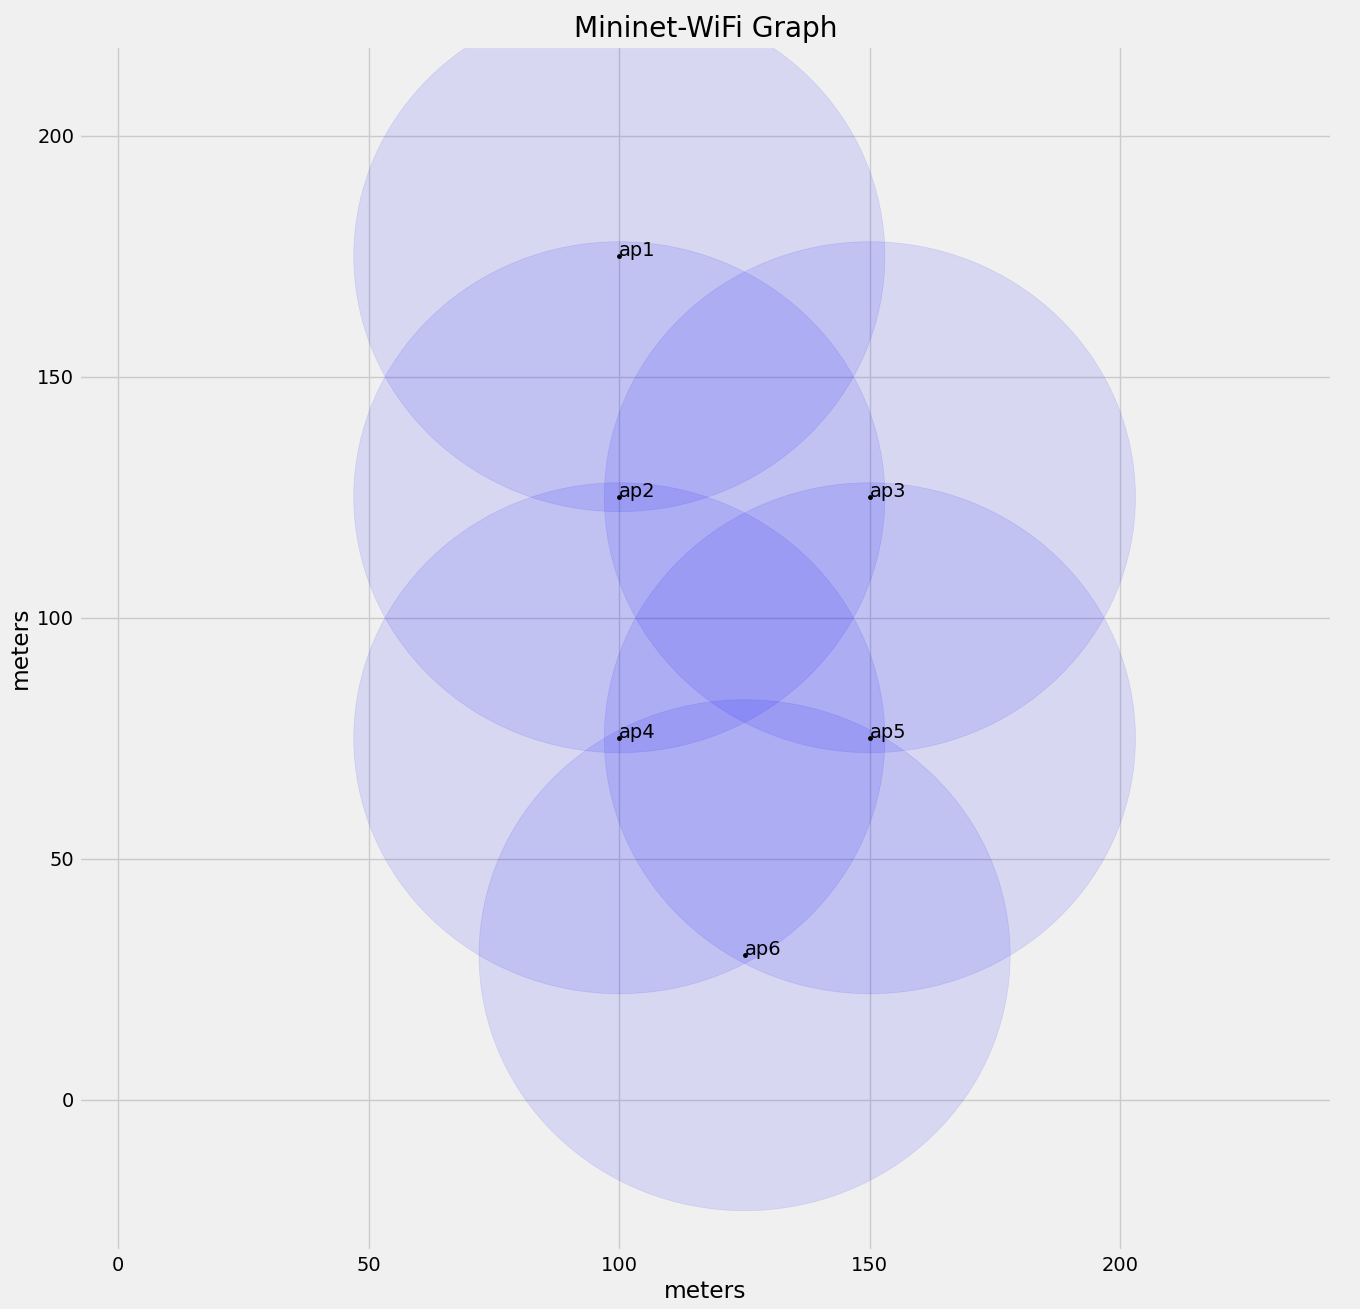
\includegraphics[width=0.9\textwidth]{fig/04_in-band/in_band_8.png}
    \caption{Topología representada por la herramienta gráfica Mininiet-WiFi.}
    \label{fig:subfiguraA}
  \end{subfigure}
  \begin{subfigure}{.49\textwidth}
    \centering
    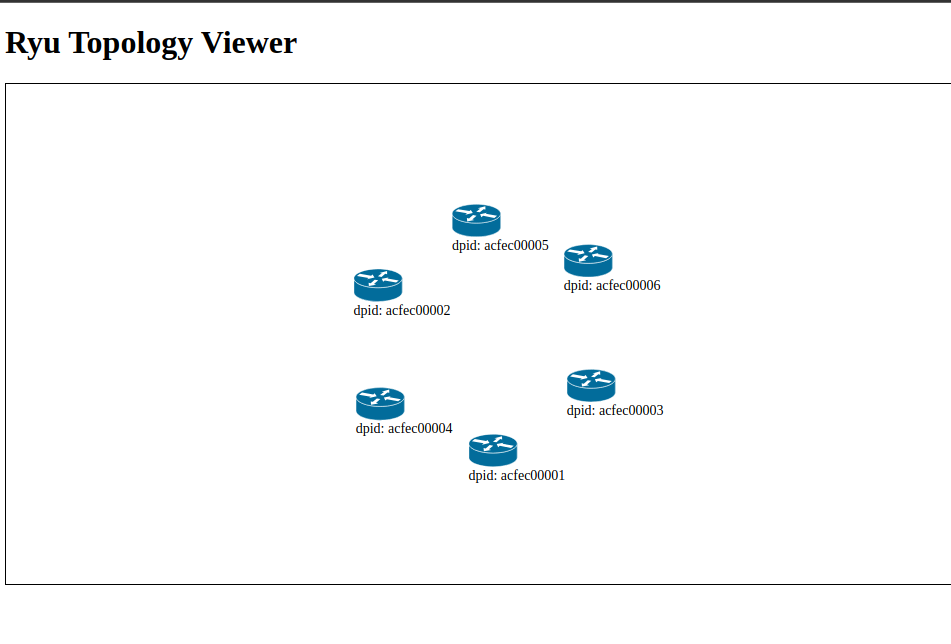
\includegraphics[width=\textwidth]{fig/04_in-band/in_band_9.png}
    \caption{Topología representada por la herramienta de descubrimiento topológico de Ryu.}
    \label{fig:subfiguraB}
  \end{subfigure}
  \caption{Topología de ejemplo elegida para el banco de pruebas.}
  \label{fig:figuraCompleta}
\end{figure}

Como puede observarse en la Figura~\ref{fig:subfiguraB}, aunque solo un dispositivo mantiene una conexión directa al controlador, este descubre correctamente el resto de los dispositivos, lo que indica que las rutas \textit{in-band} se han establecido con éxito y que el diálogo OpenFlow puede iniciarse. Hay que tener en cuenta que el visor de topología de Ryu no representa las interconexiones inalámbricas entre nodos, y además no diferencia el origen de los mensajes OpenFlow de cada dispositivo cuando todos ellos llegan a través de la misma sesión (la que mantiene el nodo raíz con el controlador). Por este motivo, en la visualización de Ryu los nodos aparecen aislados y no se muestran los enlaces inalámbricos explícitamente. En cualquier caso, la topología de ejemplo queda correctamente desplegada: todos los nodos son detectados por el controlador y las rutas \textit{in-band} necesarias se han configurado.\\
\\
Para analizar y verificar con mayor detalle el comportamiento del protocolo, se examinan las tablas generadas en cada dispositivo de la red. En primer lugar, se marca el nodo \textit{A} como raíz y se lanza el protocolo. Por un lado, se recopila la asociación \((MAC \rightarrow ID)\) creada en la tabla de vecinos por cada nodo tras el intercambio de mensajes \textit{Hello}. Por otro lado, se registran las \gls{hlmac} almacenadas en cada nodo tras el proceso de inundación de etiquetas. Estos resultados se muestran en la Figura~\ref{fig:figuraCompleta2}: la Figura~\ref{fig:subfiguraA2} contiene el resultado del proceso de intercambio de \textit{Hello}, y la Figura~\ref{fig:subfiguraB2} ilustra las rutas \gls{hlmac} almacenadas en cada nodo. Como puede apreciarse, el análisis teórico realizado en la Sección~\ref{sec:inband_proto_desc} coincide con los resultados experimentales. Por ejemplo, en la Figura~\ref{fig:subfiguraA2}, \textit{A} ha detectado un único vecino al que ha asignado el ID 1, que corresponde al nodo \textit{B}, tal y como en el ejemplo teórico. De igual modo, los nodos \textit{B}, \textit{D} y \textit{F} presentan tres vecinos, mientras que \textit{C} y \textit{E} muestran dos. Respecto a las rutas \gls{hlmac} almacenadas, la Figura~\ref{fig:subfiguraB2} reproduce los mismos resultados que el análisis teórico: por ejemplo, \textit{D} ha almacenado las rutas \textit{1.1.3}, \textit{1.1.2.2.2} y \textit{1.1.2.2.3.1}, lo que confirma que el protocolo funciona correctamente en el escenario emulado.

\begin{figure}[ht!]
  \centering
  \begin{subfigure}{.5\textwidth}
    \centering
    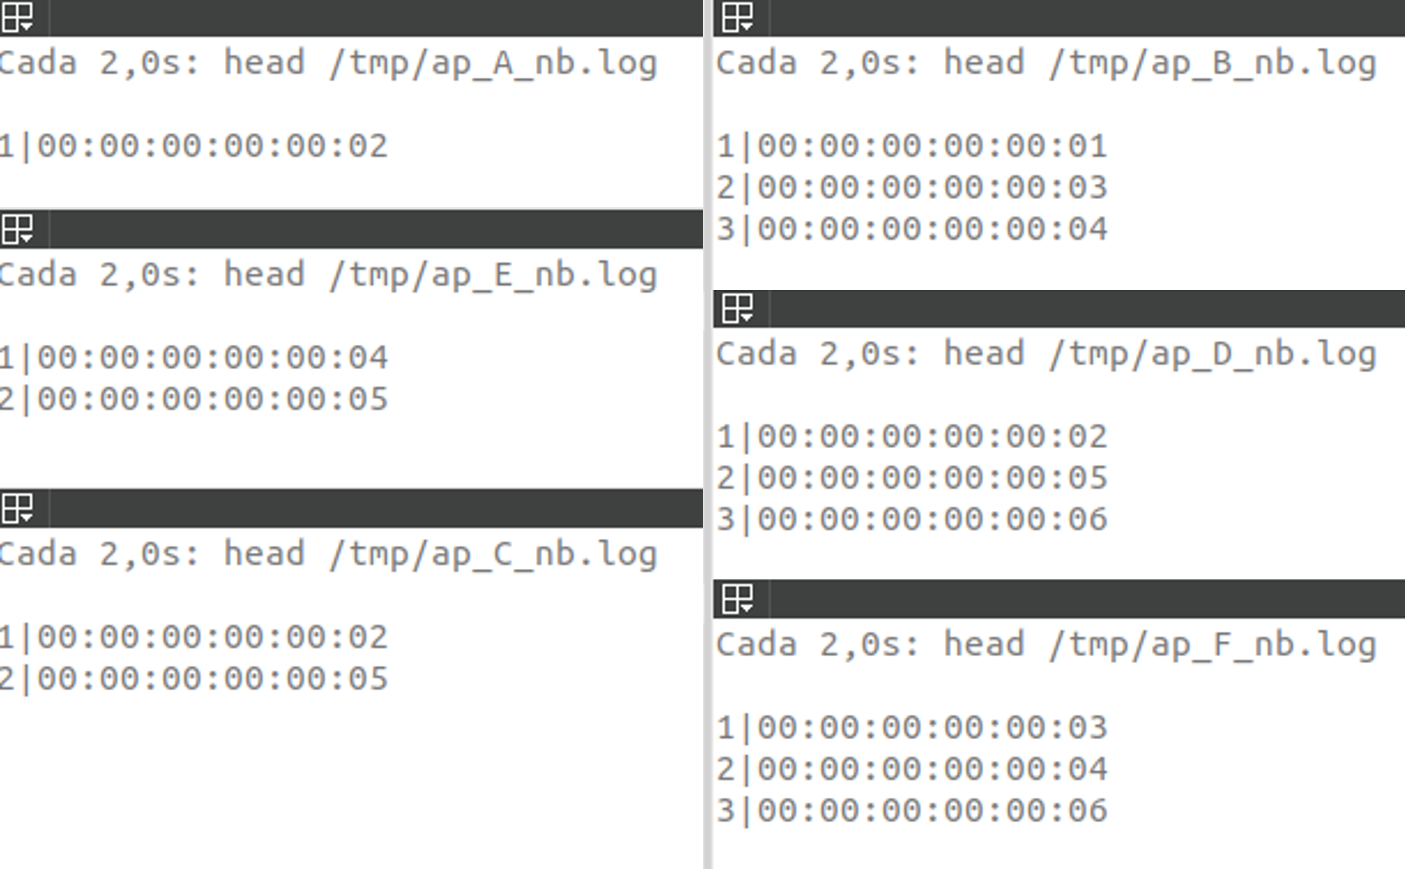
\includegraphics[width=0.95\textwidth]{fig/04_in-band/in_band_10.png}
    \caption{Tabla de vecinos.}
    \label{fig:subfiguraA2}
  \end{subfigure}%
  \begin{subfigure}{.5\textwidth}
    \centering
    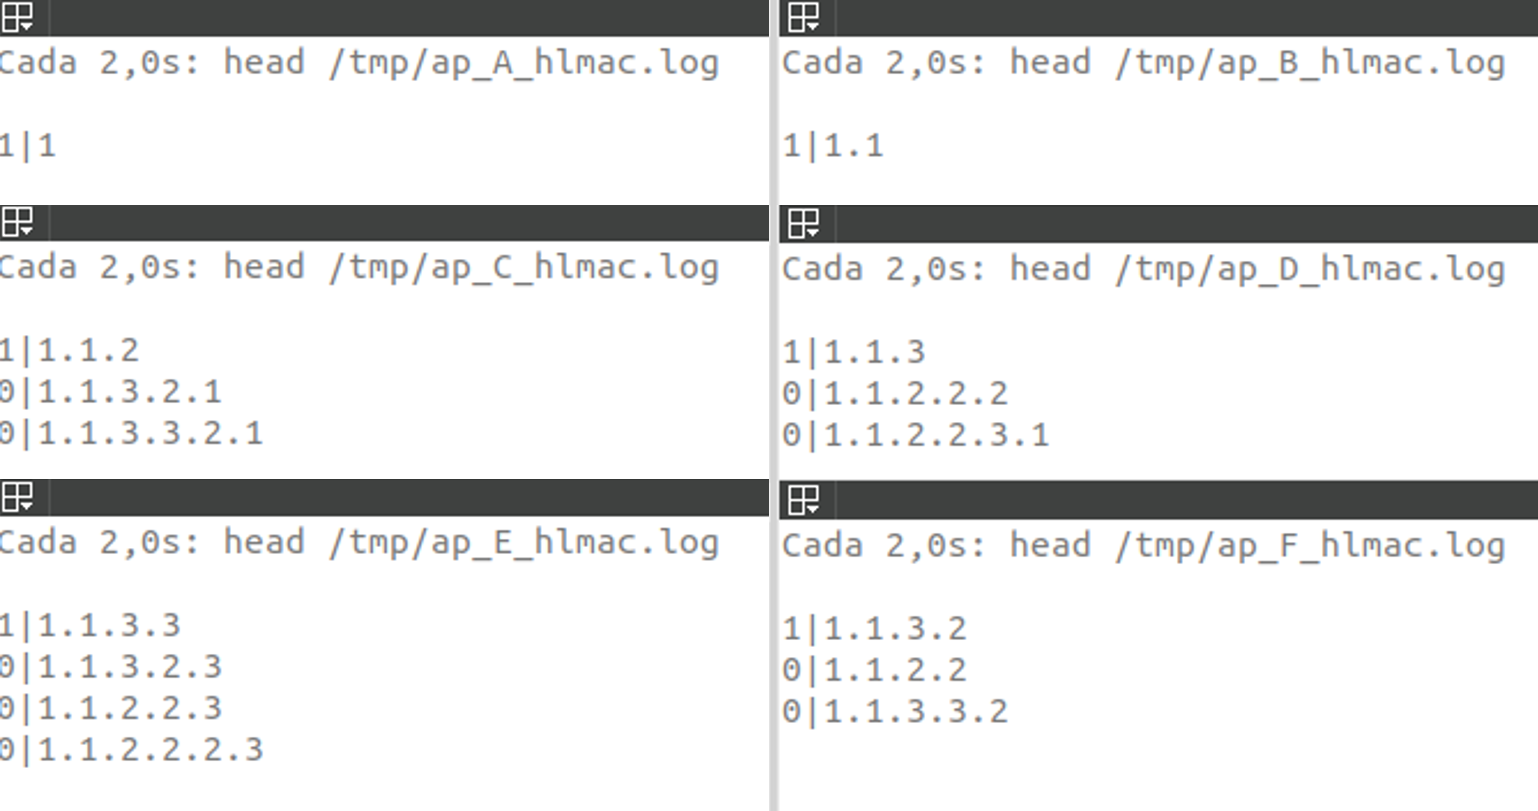
\includegraphics[width=\textwidth]{fig/04_in-band/in_band_11.png}
    \caption{Tabla HLMAC.}
    \label{fig:subfiguraB2}
  \end{subfigure}
  \caption{Prueba funcional de la implementación en la topología básica de ejemplo.}
  \label{fig:figuraCompleta2}
\end{figure}

\section{Conclusiones}

En este trabajo hemos definido e implementado un protocolo de control \textit{in-band} específicamente diseñado para su aplicación en entornos \gls{sdn} inalámbricos, prestando especial atención a los dispositivos \gls{iot} con recursos restringidos en el borde de la red. La implementación se ha integrado con éxito en el switch de referencia \gls{bofuss}, acuñándolo como \texttt{win-BOFUSS}, y se ha probado conjuntamente con la plataforma controladora Ryu. El protocolo requiere un número muy reducido de mensajes de señalización y mantiene compactas las entradas en las tablas de enrutamiento, lo que lo hace especialmente apropiado para dispositivos con capacidades de cómputo, memoria y energía limitadas. Además, ofrece mecanismos intrínsecos de resiliencia: se generan rutas de respaldo que permiten mantener la sesión de control y garantizar continuidad de servicio frente a fallos o escenarios de movilidad. En conjunto, esta aportación constituye una base sólida para futuros desarrollos orientados al despliegue del \textit{cloud continuum} y al uso del etiquetado jerárquico para establecer encaminamiento autónomo.
\chapter{DEN2NE}
\label{ch:den2ne}


Una vez sentadas las bases del etiquetado jerárquico como mecanismo habilitador de exploración y creación de canales de control \textit{in-band} en redes inalámbricas-\gls{sdn}, con la siguiente propuesta se quiso ampliar el alcance, poniendo el foco en las redes densas, heterogéneas y distribuidas.\\
\\
En este capítulo se presenta \gls{d2e}, un algoritmo escalable para la distribución y reasignación automática de recursos en entornos distribuidos, basado también en el etiquetado jerárquico. El origen del nombre hace referencia al Pokémon tipo eléctrico/hada, llamado Dedenne, el cual, no es capaz de generar electricidad por si mismo, por lo que utiliza su cola para absorber la electricidad de los hogares y recargarse. Esta idea surgió a la par que se empezó a gestar este trabajo, el cual originalmente, iba a ser una colaboración con el Departamento de Electrónica de la UAH, enfocado en el desarrollo de soluciones de encaminamiento inteligente en redes de distribución eléctrica.\\
\\
Finalmente, la colaboración dio lugar a otro trabajo que se detallará más adelante en el Capítulo~\ref{ch:den2ne}. Sin embargo, esta propuesta siguió adelante manteniendo el nombre de \gls{d2e}, dando lugar a una solución con un marco más general y aplicable a distintos dominios de redes densas y heterogéneas, convirtiéndose en una de las principales contribuciones de esta Tesis (Carrascal \textit{et al.}~\cite{carrascal2024topology}).  

\section{Introducción}

En la era contemporánea, la globalización y los avances tecnológicos han propiciado una profunda interconexión a nivel mundial en diversos aspectos, tales como la comunicación, la logística, la provisión de servicios y la explotación de recursos naturales. Todos estos avances, englobados bajo el concepto de Internet de Todo (del inglés, \gls{ioe})~\cite{Akan23}, se caracterizan por la presencia de redes densas y nodos heterogéneos, cada uno de los cuales busca intercambiar recursos en función de sus necesidades y capacidades específicas.\\
\\
Según se pudo analizar en profundidad en la Sección~\ref{subsubsec:propuestas_recursos}, la gestión y el planeamiento de recursos en entornos densos y heterogéneos ha dado lugar a una familia diversa de soluciones, las cuales se diferenciarán en función del dominio de aplicación.\\
\\
En lo que respecta a la gestión energética, la implementación de las redes eléctricas inteligentes~\cite{Rodriguez16,Tenti23} (\gls{sg}) ha permitido optimizar el aprovechamiento de la energía generada localmente, favoreciendo la autocompensación y mejorando la eficiencia en su distribución. De forma análoga, las redes de gas natural~\cite{Midthun13} han tenido que incorporar mecanismos avanzados de control de flujo~\cite{Zlotnik15} para interconectar de manera más eficiente a productores y consumidores. En el sector servicios, tanto la logística~\cite{moreno2024multi,Chen21taxi} como las aplicaciones de \textit{food delivery}~\cite{Nguyen23,Liu19food} han evidenciado la necesidad de optimizar las rutas de reparto con el fin de reducir costes y tiempos de entrega. Por su parte, en el ámbito de las comunicaciones, la expansión del \gls{iot} y la próxima generación de las redes \gls{6g} han intensificado la interconexión de dispositivos~\cite{jiang2021road}, apoyándose en tecnologías habilitadoras como el \gls{sdn}, que proporcionan una gestión centralizada y flexible de la red. Dentro del ecosistema \gls{6g}, el paradigma de \textit{fog/edge computing} introduce un nuevo escenario en el que el recurso a intercambiar es la capacidad de cómputo~\cite{Bachiega23}, lo que requiere de algoritmos y estrategias distribuidas que permitan la cooperación eficiente entre nodos. Sin embargo, la creciente densidad y heterogeneidad de dichos nodos plantea un desafío considerable, pues las diferencias en capacidades y requisitos dificultan la gestión óptima de los recursos. Tal y como se expuso en el Capítulo~\ref{ch:problema}, abordar esta complejidad exige recurrir a algoritmos de optimización y a sistemas de gestión capaces de facilitar la toma de decisiones en la asignación de recursos, garantizando así un intercambio justo, beneficioso y equilibrado entre los diferentes actores que conforman estas redes interconectadas.\\
\\
Es por ello, que se presenta \gls{d2e}, un algoritmo novedoso para el reparto y la reasignación automática de recursos en entornos distribuidos. Aunque inicialmente se pensó para distribuir energía entre prosumidores en redes inteligentes, \gls{d2e} puede ser aplicado para cualquier entorno distribuido donde los nodos tengan que intercambiar algún recurso o colaborar en alguna tarea con objetivos comunes.  Un ejemplo típico son las redes de \textit{fog computing}, donde los dispositivos en el \textit{edge} suelen tener limitaciones de memoria o energía, por lo que la redistribución de tareas es fundamental y debe realizarse en el momento oportuno.\\
\\
La principal contribución de \gls{d2e} radica en la capacidad del algoritmo de descubrir los nodos y los recursos asociados en redes densas de múltiples saltos, esbozando posteriormente un esquema de distribución eficiente. Todo ello se logra de manera efectiva y escalable, teniendo en cuenta la topología de la red. Más específicamente, y en comparación con el estado del arte (analizado en la Sección~\ref{subsubsec:propuestas_recursos}), esta contribución puede desglosarse en los siguientes puntos:

\begin{itemize}
    \item Descubrimiento de topologías malladas mediante un procedimiento generalizado de etiquetado jerárquico, lo suficientemente versátil como para aplicarse a cualquier tipo de red.
    
    \item Identificación de una o varias rutas desde cada nodo de la red hasta el sumidero de la topología (nodo \textit{root}), lo que permite establecer caminos de respaldo en caso de fallo de nodos.
    
    \item Desarrollo de un procedimiento de asignación de recursos adaptado a redes densas de múltiples saltos, garantizando al mismo tiempo la escalabilidad (baja complejidad y tiempo de convergencia reducido).
    
    \item Diseño de seis criterios diferenciados que permiten adaptar el algoritmo a distintos tipos de escenarios en red, en función del recurso que se desee balancear. 
\end{itemize}

A partir de estas contribuciones, cabe destacar la versatilidad, la resiliencia y la escalabilidad que caracterizan a \gls{d2e}, considerando además entornos de multi-salto, lo cual representa un enfoque particularmente novedoso en el área.

\section{Definición del algoritmo}

Para explicar los objetivos y principios de diseño de nuestro algoritmo, resulta necesario en primer lugar contextualizar su motivación a través de una red compuesta por múltiples nodos que son heterogéneos y/o con recursos limitados, en la que una o varias tareas deben completarse en un tiempo determinado. Cada una de estas tareas no puede ser realizada por un único nodo de manera individual. Por tanto, en este tipo de redes, los nodos deben necesariamente delegar y cooperar para completar las tareas de forma conjunta; al mismo tiempo, deben considerar las necesidades de los demás con el fin de que la redistribución resulte lo suficientemente justa.\\
\\
La Figura~\ref{fig:den2ne_01} ilustra dos ejemplos de estas redes. En el lado izquierdo se representa una \textit{microgrid}. Los sistemas de \textit{microgrid} son redes energéticas formadas por un conjunto de prosumidores, nodos que pueden actuar tanto como productores como consumidores de electricidad, normalmente porque disponen de una fuente renovable instalada (por ejemplo, paneles solares).

\begin{figure}[ht!]
    \centering
    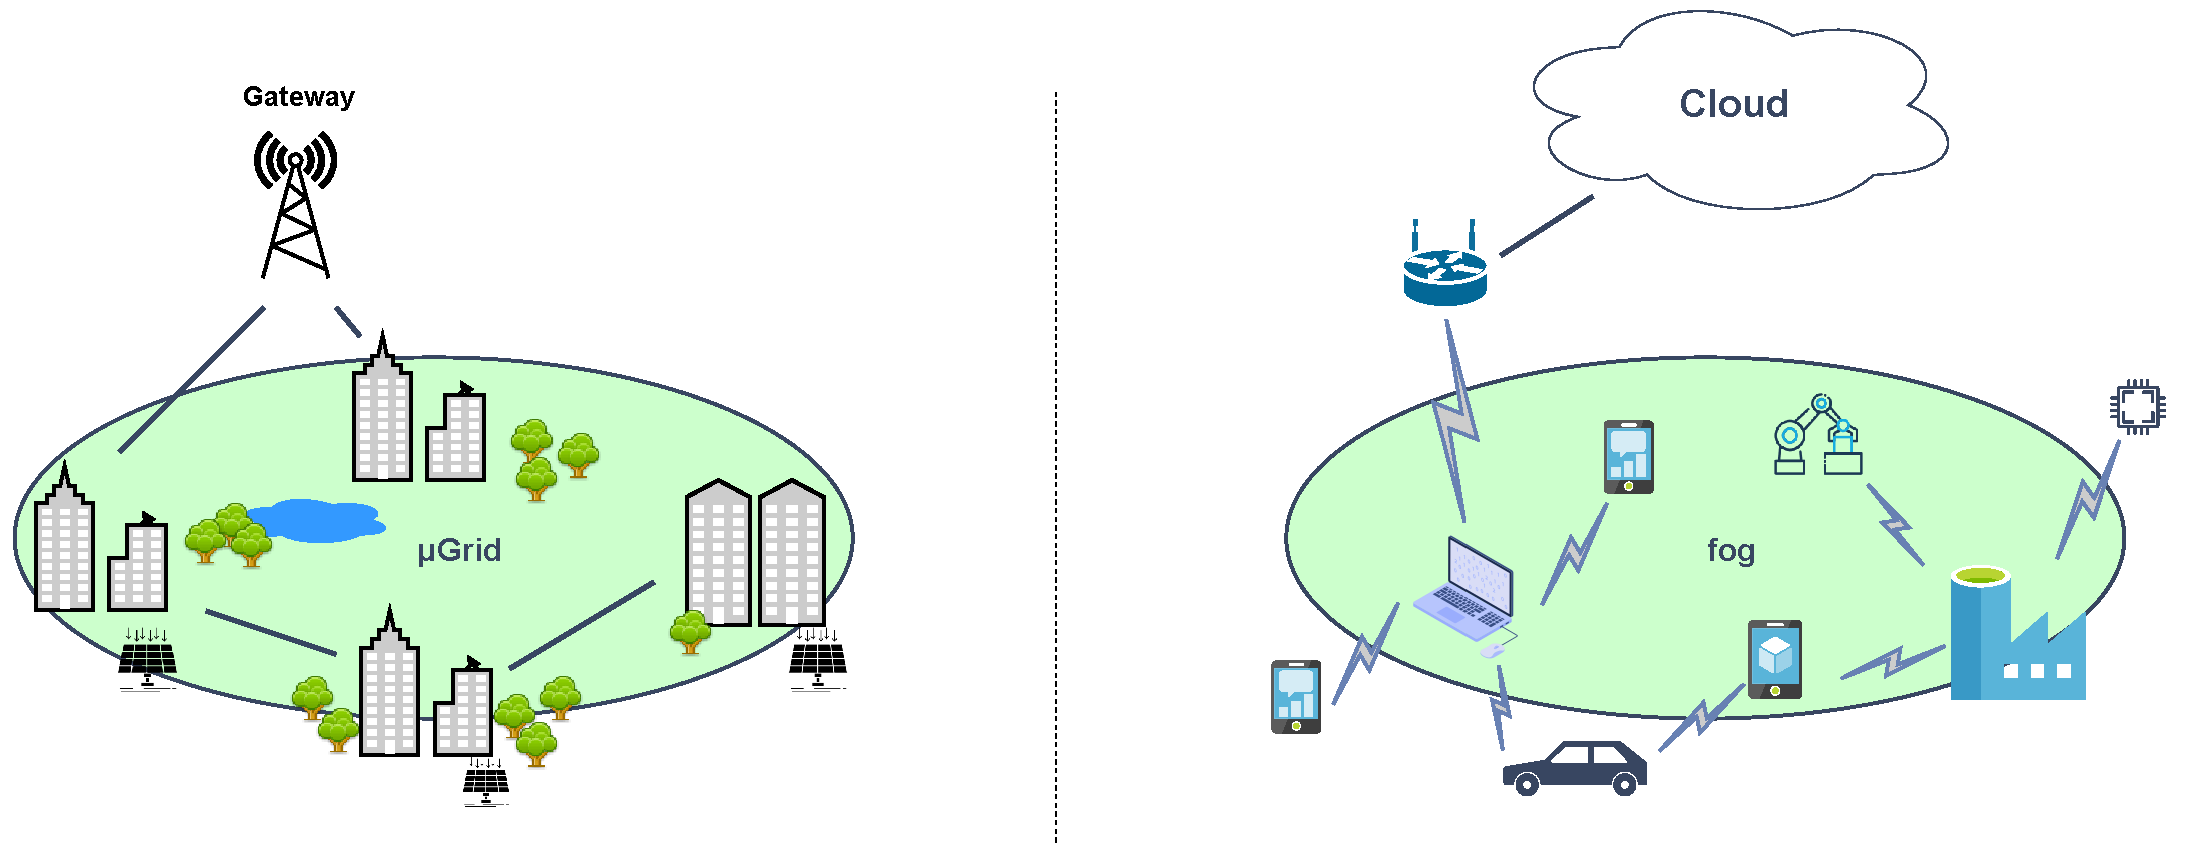
\includegraphics[width=\textwidth]{fig/05_den2ne/den2ne_01.drawio.pdf}
    \caption{Dos ejemplos de redes que aprovecharían DEN2NE para equilibrar los recursos.}
    \label{fig:den2ne_01}
\end{figure}

Estos sistemas necesitan redistribuir la producción excedente entre otros consumidores, y dicha distribución energética debe realizarse lo más cerca posible de la fuente para minimizar las pérdidas por transmisión. En la parte derecha se representa una red de \textit{fog computing}, compuesta por diversos dispositivos \gls{iot}, como ordenadores portátiles, teléfonos móviles, automóviles o robots industriales. En este último escenario, un nodo \gls{iot} podría necesitar ejecutar una tarea, y descargarla (hacer un \textit{offload}) entre otros dispositivos cercanos con recursos de cómputo disponibles podría acelerar su finalización. Como puede observarse, ambas implementaciones requieren algoritmos análogos para compartir una o varias acciones/tareas que deben completarse (por ejemplo, producción de energía, cómputo de una tarea, etc.). Además, ambos ejemplifican una porción de una red mucho mayor, lo que implica que disponen de una conexión (p. ej., un \textit{gateway}) con el resto de esa red global. Por ejemplo, una \textit{microgrid} podría usar el \textit{gateway} para enviar o recibir energía del resto del despliegue de la red inteligente, y lo mismo ocurre en el entorno \textit{fog}, que podría delegar la resolución de la tarea en la nube en el peor de los casos (es decir, cuando todos los nodos están saturados y no pueden procesarla localmente).\\
\\
En consecuencia, el objetivo principal de nuestro algoritmo es redistribuir de forma eficiente recursos entre cualquier tipo de nodos conectados. Para ello, cualquier nodo que actúe como fuente puede delegar un recurso a cualquier nodo destino. En este sentido, la formulación del problema se asemeja a un problema de encaminamiento (según se estudió en la Sección~\ref{subsubsec:conclu_recursos}), con una diferencia: en el encaminamiento hay una información que debe entregarse desde un origen concreto a un destino concreto y solo es necesario calcular la ruta; en este caso, aunque existe un origen y una información definida, los destinos potenciales pueden ser múltiples, y deben decidirse conjuntamente con la ruta que seguirá la información/recurso a distribuir. Dicho de otro modo, un recurso puede compartirse entre uno o varios nodos destino, y esa decisión debe calcularse por el algoritmo, junto con las rutas para alcanzarlos.\\
\\
Para cumplir el objetivo anterior, el diseño del \gls{d2e} se sustenta en tres principios fundamentales:

\begin{enumerate}

    \item \textbf{Tiempo de rápido convergencia}: la decisión sobre el reparto de recursos debe computarse con rapidez; es decir, el algoritmo debería presentar un tiempo de convergencia bajo. Además, dicho tiempo no debería verse penalizado de forma drástica por la cantidad de datos/recursos disponibles o por el número de nodos de la red; idealmente crecerá de manera cercana a lineal con el tamaño de la red ($\mathcal{O}(n)$). Tiempos de convergencia cortos facilitan actualizaciones ágiles en escenarios de alta movilidad.
    
    \item \textbf{Baja complejidad}: dado que los nodos que ejecutarán el algoritmo suelen ser dispositivos con recursos limitados (memoria, batería, CPU), el método debe exigir poca capacidad de cómputo y almacenamiento, e implicar un número reducido de mensajes de control intercambiados.
    
    \item \textbf{Versatilidad}: además de escalable, el algoritmo debe ser fácil de adaptar a distintos entornos prácticos (redes cableadas e inalámbricas, \gls{sg}, entornos \gls{iiot}, enfoques centralizados o distribuidos, etc.). En concreto, su diseño debe evitar supuestos demasiado restrictivos sobre la infraestructura, para permitir su reutilización en escenarios variados.
\end{enumerate}

Sobre la base de estos tres principios, se tomó como punto de partida el protocolo de encaminamiento IoTorii de Rojas \textit{et al.}~\cite{rojas2021outperforming} (Analizado en la Sección~\ref{subsubsec:propuestas_etiquetado}), ya que cumple con requisitos de convergencia rápida y bajo consumo de recursos. Aunque IoTorii está concebido como protocolo de encaminamiento, su naturaleza distribuida facilita transformarlo a una versión centralizada si fuera necesario. No obstante, dado que IoTorii selecciona rutas para pares origen–destino concretos, ha de adaptarse para satisfacer los objetivos del \gls{d2e}, que no asume un conjunto de destinos predefinidos de partida. En particular, el \gls{d2e} se diseña para localizar los vecinos más cercanos a los que se puede delegar una tarea o recurso. En este escenario se asume la existencia, de al menos, un nodo con acceso a recursos <<ilimitados>>, que actúe como sumidero de recursos de la red; a dicho nodo lo denominamos \textit{gateway} o nodo raíz (\textit{root}). Los \textit{gateway} pueden asumir la porción restante de la tarea o recurso cuando el \textit{offloading} local no sea factible. En las siguientes sub-Secciones se describirá en detalle el algoritmo \gls{d2e}.

\subsection{Terminología del algoritmo}
\label{subsec:terminologiaDEN2NE}
Una vez presentada la motivación del algoritmo y antes de profundizar en su descripción, definiremos algunos términos que se emplearán posteriormente. Para mayor claridad, nos centraremos en la Figura~\ref{fig:den2ne_02}, como ejemplo de escenario de aplicación. En dicho escenario, contamos con seis nodos (representados como círculos) conectados a un nodo raíz (\textit{root}). Los nodos están conectados bidireccionalmente (ya sea de forma cableada o inalámbrica), como indican las flechas negras bidireccionales más oscuras, y sus números simbolizan un <<recurso>> que debe ser distribuido o balanceado. Más concretamente, dicho recurso puede representar una \textbf{oferta} o una \textbf{demanda} (por ejemplo, producción/consumo eléctrico o capacidades computacionales disponibles o requeridas). En el caso de la Figura~\ref{fig:den2ne_02}, los valores negativos expresan una demanda, mientras que los positivos expresan una oferta. En este sentido, por ejemplo, una demanda de -80 se compensaría con una oferta equivalente de +80 o, alternativamente, con una combinación de ofertas que sumaran +80. Por lo tanto, el objetivo principal de nuestro algoritmo es compensar todos los recursos en la red, es decir, que todos los nodos tiendan hacia el valor cero (un uso óptimo), mientras que el remanente (ya sea exceso de demanda u oferta) se redirija hacia el nodo raíz. \\
\\
Antes de describir las tres fases del algoritmo \gls{d2e} (en las Secciones~\ref{subsec:fase1}, \ref{subsec:fase2}, y \ref{subsec:fase3}, respectivamente), reflexionemos sobre el ejemplo de la Figura~\ref{fig:den2ne_02} para entender por qué se definieron tres fases. Considerando los principios de diseño mencionados anteriormente, calcular todas las posibles combinaciones de reparto no es factible en un tiempo razonable. Por otro lado, la información local podría reducir los tiempos de convergencia y la complejidad, pero tampoco sería suficiente para decidir de manera óptima. Como ejemplo de una mala decisión, el nodo con una demanda de -80 solo conoce a sus dos vecinos: uno que ofrece (+100) y otro que demanda (-10), y podría pensar que el nodo más adecuado para cubrir su demanda (-80) es el vecino inferior (+100) (en la Figura~\ref{fig:den2ne_02}). Sin embargo, esta decisión local resulta ser incorrecta, ya que existen otros nodos con demandas adicionales (-50, -40 y -30), que también requieren de esa oferta y se encuentran mucho más alejados del nodo raíz. De hecho, la solución de distribución óptima se ilustra con flechas naranjas claras (que representan la dirección desde el nodo demandante hacia el nodo con oferta). Esta distribución implicaría que todos los nodos quedaran balanceados en cero y que la demanda restante de -110 (suma de -50 -40 -30 +100 -80 -10) se desviara hacia el nodo raíz, el cual, sería capaz de cubrirla.


\begin{figure}[ht!]
    \centering
    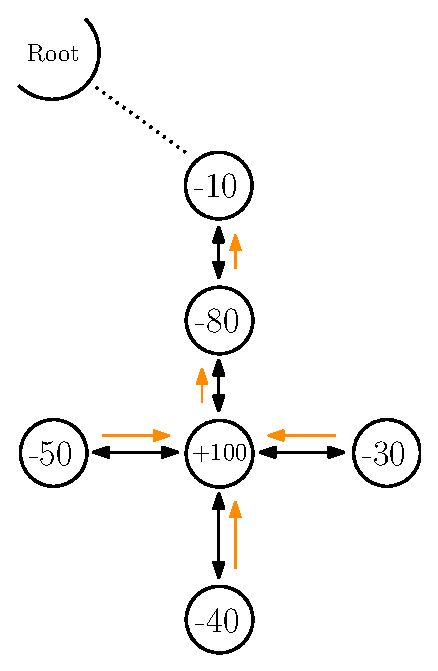
\includegraphics[width=0.4\textwidth]{fig/05_den2ne/den2ne_02.eps}
    \caption{Ejemplo de equilibrio de recursos en una red con seis nodos y un \textit{gateway} (o nodo raíz).}
    \label{fig:den2ne_02}
\end{figure}

Consecuentemente, el algoritmo \gls{d2e} calcula la distribución de recursos considerando información de todos los nodos atravesados, en lugar de limitarse únicamente a la información local de los vecinos. Además, prioriza la distribución en los nodos más alejados del nodo raíz, arrastrando el remanente (oferta o demanda) hacia la raíz para que pueda ser compensado allí por el resto de la red (por ejemplo, la nube o la \textit{smartgrid}).\\
\\
En las subsecciones siguientes se describen en detalle las tres fases que componen el algoritmo. La primera fase está dedicada a explorar la topología y agregar información de los nodos recorridos mediante etiquetado jerárquico; la segunda selecciona, entre todas las etiquetas recibidas, el conjunto de información que parece más cercano a la solución óptima; y la tercera ejecuta el balance de recursos en función de la decisión tomada en la fase segunda. Más concretamente:

\begin{itemize}
    \item En la \textbf{Fase 1} (Subsección~\ref{subsec:fase1}) se explica el etiquetado jerárquico para calcular rutas desde cada nodo hasta el nodo raíz. Esta fase se inspira en los trabajos relacionados sobre encaminamiento escalable y resiliente examinados en la Sección~\ref{subsubsec:propuestas_etiquetado}.
    
    \item En la \textbf{Fase 2} (Subsección~\ref{subsec:fase2}), una vez que se han generado todas las rutas posibles hacia la raíz, se selecciona, en cada nodo, una de ellas siguiendo un criterio concreto. Este criterio proporciona la versatilidad prevista como principio de diseño: proponemos seis criterios para que el más adecuado se aplique según el escenario, aunque en la práctica cualquier otro criterio nuevo podría emplearse si fuese necesario.
    
    \item En la \textbf{Fase 3} (Subsección~\ref{subsec:fase3}), tras la selección de la ruta activa ($ID_{activa}$) en la fase anterior, se realiza el balanceo de recursos en base a la lista de nodos representada por las etiquetas activas. Esta fase tiene en cuenta además las condiciones reales de la red, por ejemplo, si los enlaces presentan pérdidas o capacidades limitadas.
\end{itemize}


\subsection{Fase 1 - Etiquetado jerárquico}
\label{subsec:fase1}

El algoritmo \gls{d2e} comienza localizando las posiciones relativas de cada nodo en la red. Para ello, se realiza un etiquetado jerárquico a partir de cada nodo raíz presente en el despliegue. Como algoritmo centralizado, cada nodo dispone de un identificador numérico único (ID) que les identifica en la red, y obtienen durante el proceso una etiqueta jerárquica que les indicará su posición en la topología, y una ruta para alcanzar el sumidero de la misma. Este mecanismo de etiquetado jerárquico comparte ciertos aspectos con el descrito en el Capítulo~\ref{ch:propuestaInband}, sin embargo, en vez de emplear un etiquetado basado en sufijos auto-asignados en procesos de reconocimiento de vecindad, se emplearán identificadores únicos, aligerando el proceso de exploración de la topología. La Figura~\ref{fig:den2ne_03} presenta el esquema de etiquetado diseñado. 


\begin{figure}[ht!]
    \centering
    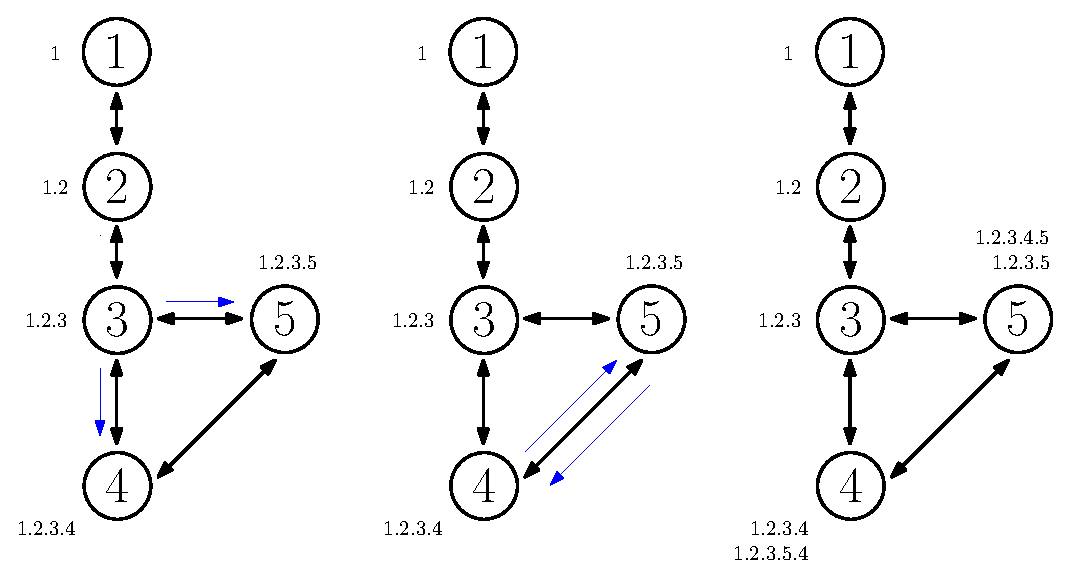
\includegraphics[width=0.9\textwidth]{fig/05_den2ne/den2ne_03.eps}
    \caption{Procedimiento de etiquetado jerárquico en DEN2NE.}
    \label{fig:den2ne_03}
\end{figure}

El procedimiento parte en el nodo raíz, que en la Figura~\ref{fig:den2ne_03} tiene ID~1 y un vecino conectado con ID~2. Para correlacionarlos jerárquicamente, el algoritmo asigna la etiqueta \texttt{1} al raíz y concatena el ID del vecino a la suya propia, de modo que el nodo~2 recibe la etiqueta \texttt{1.2}. A continuación, el nodo con ID~3 obtendrá la etiqueta \texttt{1.2.3}, y los nodos con IDs~4 y~5 recibirán las etiquetas \texttt{1.2.3.4} y \texttt{1.2.3.5}, respectivamente. Además, conforme progresa la asignación, el nodo con ID~4 también podrá registrar la etiqueta \texttt{1.2.3.5.4} y el nodo con ID~5 la etiqueta \texttt{1.2.3.4.5}, según correspondan las rutas alternativas. Este procedimiento de etiquetado continúa hasta que se explora toda la red y cada nodo dispone, al menos, de una etiqueta jerárquica. En la práctica, cada etiqueta representa una ruta para alcanzar el nodo raíz, por lo que, nodos con múltiples rutas tendrán capacidad de balancear sus recursos por rutas alternativas.\\
\\
Para evitar bucles durante la fase de etiquetado jerárquico, el algoritmo no asigna a un nodo etiquetas que lo hereden de sí mismo. Esto se puede prever fácilmente ya que las etiquetas concatenan los IDs de los nodos recorridos, por lo que ninguna etiqueta debe contener un mismo ID repetido; de lo contrario, indicaría la existencia de un bucle en la ruta. Por ejemplo, la Figura~\ref{fig:den2ne_04} ilustra gráficamente esta restricción y muestra el siguiente paso respecto a lo representado en la Figura~\ref{fig:den2ne_03}. Cuando el nodo con ID~4 recibe la etiqueta \texttt{1.2.3.5.4} del nodo con ID~5, podría intentar propagar la etiqueta \texttt{1.2.3.5.4.3} hacia el nodo con ID~3, pero esta acción no se realiza porque la etiqueta contiene el ID~3 en dos ocasiones, lo que representaría un bucle. Una vez descartada dicha etiqueta, no se propagarán más etiquetas que la deriven. De manera análoga, si el nodo con ID~5 generara \texttt{1.2.3.4.5.3} para el nodo~3, esta también sería rechazada por el mismo motivo. En este ejemplo concreto, tras estos pasos descritos, no se asignan más etiquetas y el procedimiento del etiquetado jerárquico habría concluido en este punto.


\begin{figure}[ht!]
    \centering
    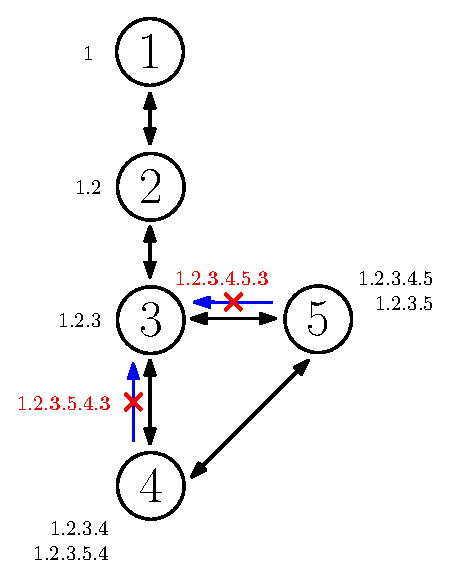
\includegraphics[width=0.4\textwidth]{fig/05_den2ne/den2ne_04.eps}
    \caption{Mecanismo de evitación de bucles durante el etiquetado jerárquico.}
    \label{fig:den2ne_04}
\end{figure}

Como se indicó anteriormente, cada etiqueta asignada representa una ruta hacia la raíz y cada nodo obtiene una o varias etiquetas (es decir, múltiples rutas hacia el nodo raíz). Por tanto, esta primera fase del algoritmo puede calcular, en principio, todas las rutas posibles desde cualquier nodo de la red hasta la raíz. Esto puede conllevar miles o incluso millones de rutas, según la conectividad de la topología. Por ello, desde el punto de vista de la implementación, la fase de etiquetado jerárquico suele limitarse a aprender únicamente un subconjunto de etiquetas y descartar el resto siguiendo ciertos parámetros, como la disjunción de rutas o un número mínimo de saltos~\cite{Lopez-Pajares19}. El Algoritmo~\ref{alg:labeling} resume todo el procedimiento de la Fase 1, el cual, toma como entrada el grafo de la red y el nodo desde el que se inicia el etiquetado jerárquico (es decir, el nodo raíz) y devuelve el grafo con la asignación de etiquetas correspondiente. El algoritmo recorre los nodos partiendo de los vecinos del nodo raíz. Un nodo puede ser procesado más de una vez, hasta un máximo de etiquetas asignadas (\(\textup{IDs\_MAX}\)) o hasta que se detecte un bucle (\(\textit{check\_loop()}\)). Por este motivo, podemos afirmar que la complejidad de la fase de etiquetado es \(\mathcal{O}(n)\), ya que crece de forma lineal con el número de nodos \(n\), cada uno visitado como máximo \(\textup{IDs\_MAX}\) veces; dado que \(\textup{IDs\_MAX}\) se considera una constante de diseño, la complejidad asintótica se mantiene en \(\mathcal{O}(n)\) independientemente de la forma o tamaño de la topología.


\begin{algorithm}[ht!]
\caption{Proceso de etiquetado jerárquico}\label{alg:labeling}
\SetKwInOut{Input}{input}
\SetKwInOut{Output}{output}
\Input{$\: G(\mathcal{N}, \mathcal{L}),\: root$}
\Output{$\: G(\mathcal{N}, \mathcal{L})$}
\vspace{0.2cm}
$\textup{init}\: nodes\_to\_attend$\;
$\mathcal{N}(root).push(\texttt{ID}(\textup{None}, root))$\;
$nodes\_to\_attend.push(\mathcal{N}(root))$\;
\vspace{0.2cm}
\While{$length(nodes\_to\_attend) > \emptyset$}{
\vspace{0.1cm}
$curr\_node \: = \: nodes\_to\_attend[0]$\;
\vspace{0.1cm}  
\For{$j \: \gets \: length(curr\_node.ids)$}{
    \vspace{0.1cm}  
    \uIf{$not \: curr\_node.ids[j].used$}{
        \vspace{0.1cm}  
        \For{$neighbor \: \gets \: curr\_node.neighbors$}{
            \vspace{0.1cm}
            \uIf{$check\_loop(curr\_node.ids[j], neighbor)$}{
                $\textup{pass}$\;
            }
            \uElseIf{$neighbor.ids \:  \geq \textup{IDs\_MAX}$}{
                $\textup{pass}$\;
            }
            \Else{
                $\mathcal{N}(neighbor).push(\texttt{ID}(curr\_node.ids[j], neighbor))$\;
            }
            \vspace{0.1cm}
            $nodes\_to\_attend.push(\mathcal{N}(neighbor))$\;
        }
        \vspace{0.1cm}
        $curr\_node.ids[j].used \: = \: \textup{true}$\;
    }
}

  $pop\: nodes\_to\_attend[0]$\;
  
}
\vspace{0.1cm}
\Return{$G(\mathcal{N}, \mathcal{L})$}
\end{algorithm}


\subsection{Fase 2 - Selección de las mejores etiquetas o identificadores jerárquicos}
\label{subsec:fase2}

Como se ha presentado anteriormente, los nodos raíz o \textit{gateways} son aquellos conectados a recursos externos (energía, capacidad de cómputo, etc.) que pueden considerarse prácticamente <<ilimitados>>. Por este motivo, al repartir una tarea o recurso, los nodos más alejados del nodo raíz tienen menor probabilidad de disponer de recursos locales, mientras que los nodos próximos a la raíz pueden delegar con facilidad en el \textit{gateway} para completar la operación. La primera fase del algoritmo aporta precisamente la localización relativa de los nodos respecto a la raíz/raíces, lo que permite priorizar de forma natural qué nodos deben considerarse preferentes a la hora de decidir dónde delegar una tarea; en suma, simplifica y ordena el proceso de toma de decisiones.\\
\\
Concretamente, una vez finalizado el etiquetado jerárquico, cada nodo dispone de una o varias etiquetas que representan rutas hacia la raíz, dado que cada etiqueta codifica la lista de nodos a atravesar para alcanzarla. Si un nodo cuenta con una única etiqueta, existe un único camino conocido hacia la raíz; si dispone de varias, hace falta aplicar criterios de selección para escoger la ruta más adecuada. Dado que las rutas hacia la raíz se construyen de forma coordinada entre nodos, ese criterio de selección debe aplicarse respetando un cierto orden y coordinación entre los participantes.\\
\\
La segunda fase del algoritmo, por tanto, decide dónde distribuir los recursos aplicando criterios sobre las etiquetas o identificadores jerárquicos obtenidos en la primera fase. Como referencia, el algoritmo \gls{d2e} incorpora seis criterios distintos (basados en la literatura) para puntuar cada ruta disponible: cada criterio calcula un coste asociado a una etiqueta concreta (denotado $Cost_{ID}$). A continuación, se selecciona la ruta activa, el identificador jerárquico activo $ID_{activa}$, como la que minimiza dicho coste, tal y como se expresa en la Ecuación~\ref{eq:IDactiveCost}.

\begin{align}\label{eq:IDactiveCost}
     \left \langle ID_{activa} \right \rangle  \: &  = \: min(Cost_{ID})
\end{align}

Los seis criterios se describen en las secciones siguientes. Es importante remarcar que pueden definirse e incorporar criterios adicionales al algoritmo: la segunda fase únicamente exige la especificación de una función de coste para cada criterio, por lo que la elección concreta no limita el funcionamiento del método y, de hecho, dota de versatilidad a la propuesta. Asimismo, algunos criterios resultan aplicables de forma genérica a múltiples casos de uso, mientras que otros son específicos de dominios concretos (p. ej. \gls{sg}, \textit{fog computing}, etc.). Por estas razones, los criterios se presentan de forma concisa y directa a modo de referencia; en la práctica, \gls{d2e} es potencialmente agnóstico respecto al criterio seleccionado.

\subsubsection{Criterio 1 - Número de saltos}

Este primer criterio evalúa el número de saltos necesarios para alcanzar el nodo raíz, de modo que en cada nodo se selecciona el identificador jerárquico con menor número de saltos. Se basa en el clásico criterio de camino más corto para encaminamiento en redes de comunicaciones, denominado \emph{widest-shortest path}, Ma \textit{et al.}~\cite{Ma97}. Por tanto, la función de coste para este criterio puede expresarse como en la Ecuación~\ref{eq:criterionCost01}. 

\begin{equation}\label{eq:criterionCost01}
     Cost_{ID}  \: = \: length(ID) \: - \: 1
\end{equation}
\vspace{0.2cm}

Para comprenderlo, la Figura~\ref{fig:den2ne_05} muestra un ejemplo en el que el nodo 5 ha adquirido tres identificadores jerárquicos y se representan las tres rutas potenciales hacia la raíz (nodo 1). En este escenario, el coste se calcula como la longitud del identificador (donde la longitud es el número de cifras en la etiqueta jerárquica) menos uno; por ejemplo, para el identificador \texttt{1.2.3.5} el coste es $3 = 4 - 1$, dado que dicho identificador tiene 4 cifras. Una vez calculado el coste para cada identificador jerárquico, el identificador seleccionado en el ejemplo es \texttt{1.2.3.5} conforme a la Ecuación~\ref{eq:IDactiveCost}, pues presenta el menor coste, lo que implica menos saltos para alcanzar la raíz. En caso de fallo o indisponibilidad de esa ruta principal, cualquiera de las rutas restantes podría emplearse, ordenadas por coste. 

\begin{figure}[ht!]
    \centering
    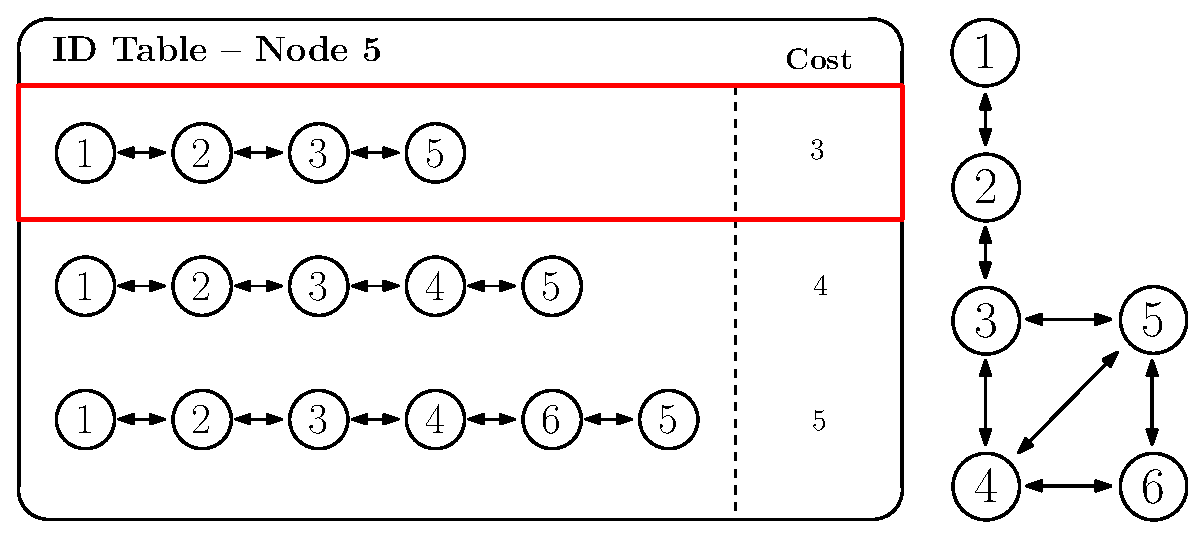
\includegraphics[width=0.9\textwidth]{fig/05_den2ne/den2ne_05.eps}
    \caption{Selección de ID basada en el criterio del número de saltos.}
    \label{fig:den2ne_05}
\end{figure}


\subsubsection{Criterio 2 - Distancia}

El segundo criterio incorpora el concepto de distancia entre nodos. Dicha distancia puede ser física (por ejemplo, en despliegues de \textit{microgrids}, donde la distancia física es conocida y constante porque los nodos no son móviles) o lógica (por ejemplo, un coste de enlace basado en el rendimiento o la latencia en un despliegue de red). Al igual que el criterio anterior, se inspira en técnicas clásicas de encaminamiento en redes de comunicaciones y recibe el nombre de \textit{shortest-distance path}, Ma \textit{et al.}~\cite{Ma97}. En este caso, el coste de cada identificador jerárquico se calcula como la suma de las distancias de los enlaces recorridos, tal como se expresa en la Ecuación~\ref{eq:criterionCost02} (una ``distancia'' puede equivaler también al inverso del \textit{throughput} del enlace u otra métrica relacionada).

\begin{equation}\label{eq:criterionCost02}
     Cost_{ID}  \: = \: \sum_{i=0}^{N_{saltos}-1} d_{i}
\end{equation}
\vspace{0.2cm}

La Figura~\ref{fig:den2ne_06} muestra el mismo ejemplo anterior aplicado con este segundo criterio. En dicho escenario, el identificador \texttt{1.2.3.5} resulta seleccionado si se cumple la condición indicada en la Ecuación~\ref{eq:criterionCost02_b}; no obstante, dependiendo de los valores reales de las distancias, podría seleccionarse cualquier otro identificador aunque la ruta tenga más saltos hasta la raíz.

\begin{equation}\label{eq:criterionCost02_b}
     \left \langle ID_{1} = ID_{activa} \right \rangle \Leftrightarrow 
     \left\{\begin{matrix}
      [d_{35} < ( d_{34} + d_{45})] \\
      \\
       \wedge \\ 
       \\
      [d_{35} < ( d_{34} + d_{46} + d_{65})] 
      \end{matrix}\right.
\end{equation}
\vspace{0.2cm}

\begin{figure}[ht!]
    \centering
    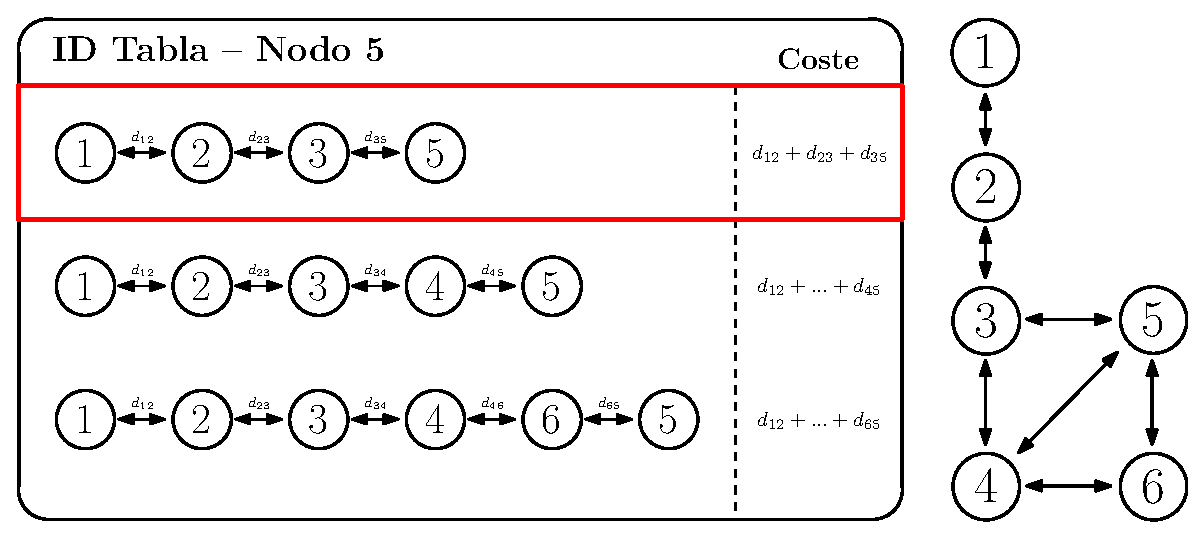
\includegraphics[width=0.9\textwidth]{fig/05_den2ne/den2ne_06.eps}
    \caption{Selección de ID basada en el criterio de distancia.}
    \label{fig:den2ne_06}
\end{figure}

\subsubsection{Criterio 3 - Pérdidas de enlace}

El tercer criterio está directamente relacionado con el caso de uso de redes inteligentes de distribución eléctrica (inspirado en la topología IEEE 123-node test feeder~\cite{Schneider17}) en el que puede aplicarse este algoritmo, y se vincula asimismo con el criterio anterior sobre distancia. Concretamente, se persigue la minimización de las pérdidas en los enlaces debidas a la transmisión. Para distinguirlo del criterio 2, conviene subrayar que el criterio 2 suele centrarse en características del enlace o su capacidad (p. ej. rendimiento o distancia), mientras que el criterio 3 atiende al efecto de degradación del enlace (p. ej. pérdidas de potencia). No obstante, ambos criterios están estrechamente relacionados y, de hecho, su formulación es conceptualmente similar, intercambiando distancias por pérdidas, como se muestra en la Ecuación~\ref{eq:criterionCost05}.

\begin{equation}\label{eq:criterionCost05}
      Cost_{ID}  \: = \: \sum_{ij}^{N_{ID}} L_{ij} \: = \: \sum_{ij}^{N_{ID}} (\frac{\alpha_{R_{ij}} \: \times \: d_{ij}}{V_{d}^{2}}\: \times \: P_{in}^{2})
\end{equation}
\vspace{0.2cm}

En el caso específico de las redes eléctricas, las pérdidas se calculan a partir de modelos de pérdidas en líneas de transmisión que consideran parámetros tales como: tensión ($V_{d}$), distancia física ($d_{ij}$), coeficiente de reflexión ($\alpha_{R_{ij}}$) y potencia de entrada ($P_{in}$), tal y como recoge la Ecuación~\ref{eq:criterionCost04_b} (incorporada en la Ecuación~\ref{eq:criterionCost05}). Como puede apreciarse, la distancia física es uno de los parámetros que afectan al coste, pero no el único. Por ello, como hemos mencionado antes, los criterios 2 y 3 están relacionados pero no necesariamente producen el mismo resultado, pues intervienen factores adicionales. En otros escenarios, las ``pérdidas'' podrían interpretarse de forma análoga (p. ej. fiabilidad de enlace en un entorno inalámbrico para computación).

\begin{equation}\label{eq:criterionCost04_b}
     L_{ij} \: = \: \frac{\alpha_{R_{ij}} \: \times \: d_{ij}}{V_{d}^{2}}\: \times \: P_{in}^{2}
\end{equation}
\vspace{0.2cm}

En el ejemplo concreto de la Figura~\ref{fig:den2ne_07}, la ruta hacia el nodo raíz seleccionada como $ID_{activa}$ es la primera (\texttt{1.2.3.5}), que en este caso coincide con la escogida por el criterio anterior. Siempre y cuando, la condición indicada en la Ecuación~\ref{eq:criterionCost05_b} se cumpla. 

\begin{equation}\label{eq:criterionCost05_b}
       \left \langle ID_{1} = ID_{active} \right \rangle \Leftrightarrow 
       \left\{\begin{matrix}
       [\sum_{\substack{1 \leq i \leq 3\\ 2 \leq j \leq 5\\ j \neq 4}}^{} L_{ij} < \sum_{\substack{1 \leq i \leq 4 \\  2 \leq j \leq 5}}^{} L_{ij}]\\
       \\
       \wedge \\ 
       \\
       [\sum_{\substack{1 \leq i \leq 3\\ 2 \leq j \leq 5\\ j \neq 4}}^{} L_{ij} < \sum_{\substack{1 \leq i \leq 5 \\ 2 \leq j \leq 6}}^{} L_{ij}]
       \end{matrix}\right.
\end{equation}
\vspace{0.2cm}

\begin{figure}[ht!]
    \centering
    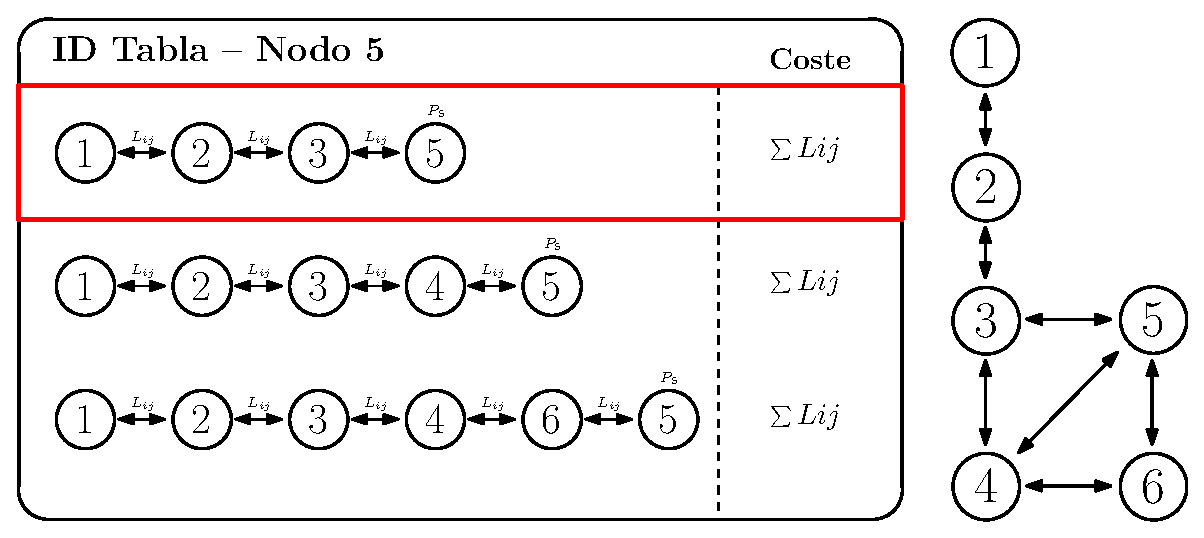
\includegraphics[width=0.9\textwidth]{fig/05_den2ne/den2ne_07.eps}
    \caption{Selección de ID basada en el criterio de pérdidas de enlace.}
    \label{fig:den2ne_07}
\end{figure}

\subsubsection{Criterio 4 - Balance de potencia}

El cuarto criterio evalúa las rutas con más recursos disponibles en su recorrido, y las selecciona preferentemente frente a otras. Dado que cada nodo puede tener una oferta de recursos (valor positivo) o una demanda (valor negativo), la suma de todos los valores a lo largo de la ruta representará un coste total de la misma, tal y como se define en la Ecuación~\ref{eq:criterionCost03}. Este coste se calcula cambiando el signo de la suma de todas las potencias en el trayecto, ya que nuestro objetivo es minimizarlo. Por lo tanto, si existen muchas ofertas de recursos, la suma será un valor positivo elevado y, al invertir su signo, se traducirá en un valor muy negativo (es decir, un bajo coste). Es importante destacar que el nombre de este criterio proviene del caso de uso de las redes eléctricas inteligentes, en el que los recursos son la potencia eléctrica. Sin embargo, aunque en la fórmula se considere la oferta y la demanda de potencia, otros parámetros, como la capacidad de cómputo en entornos de \gls{cec}, podrían aplicarse de manera análoga en este criterio.  De hecho, en el campo del enrutamiento clásico, Ma~\textit{et al.}~\cite{Ma97} lo denominan \textit{shortest-widest path}.
\begin{equation}\label{eq:criterionCost03}
     Cost_{ID}  \: = \: -(\sum_{i}^{N_{ID}} P_{i})
\end{equation}

Una vez más, la selección de $ID_{activa}$ se basará en el valor mínimo de $Cost_{ID}$. En el caso de nuestro ejemplo, como se observa en la Figura~\ref{fig:den2ne_08}, el ID seleccionado es \texttt{1.2.3.4.6.5}, el cual debería cumplir con la condición de la Ecuación~\ref{eq:criterionCost03_b}.

\begin{equation}\label{eq:criterionCost03_b}
\begin{split}
     \left \langle ID_{3} = ID_{activa} \right \rangle \Leftrightarrow
     \left\{\begin{matrix}
     [\sum_{i}^{6}P_{i} > \sum_{i}^{5}P_{i}]\\
       \\
       \wedge \\ 
       \\
       [\sum_{i}^{6}P_{i} > \sum_{i,i\neq 4}^{5}P_{i}]
     \end{matrix}\right.
\end{split}
\end{equation}
\begin{figure}[ht!]
    \centering
    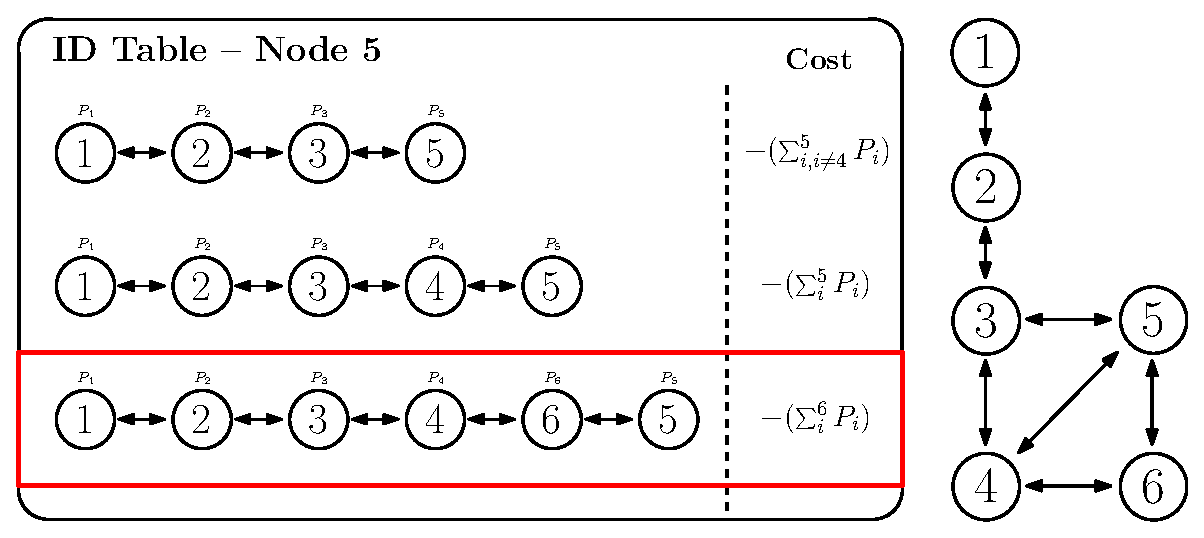
\includegraphics[width=0.9\textwidth]{fig/05_den2ne/den2ne_08.eps}
    \caption{Selección de ID basada en el criterio de balance de potencia.}
    \label{fig:den2ne_08}
\end{figure}

\subsubsection{Criterio 5 - Balance de potencia con pérdidas}

El quinto criterio combina los criterios 3 y 4~\cite{Schneider17,Ma97}, ya que busca maximizar los recursos disponibles en la ruta, al mismo tiempo que limita las pérdidas potenciales que una ruta específica (especialmente si es más larga que otras), pueda conllevar. Una vez más, en el caso de las redes eléctricas inteligentes, esto se traduce en la oferta y la demanda de potencia, restando las pérdidas en la ruta (que siguen la Ecuación~\ref{eq:criterionCost04_b}), tal y como se representa en la Ecuación~\ref{eq:criterionCost04}.  
 

\begin{equation}\label{eq:criterionCost04}
     Cost_{ID}  \: = \: -(\sum_{i}^{N_{ID}} P_{i} - \sum_{ij}^{N_{ID}-1} L_{ij})
\end{equation}
\vspace{0.2cm}

Cuando este criterio se aplica al ejemplo de la Figura~\ref{fig:den2ne_09}, la ruta seleccionada es \texttt{1.2.3.4.5}, que en realidad representa una decisión intermedia entre el criterio 3 (pérdidas en los enlaces) y el criterio 4 (balance de potencia). En consecuencia, debe cumplirse la condición de la Ecuación~\ref{eq:criterionCost04_c} para que el $ID_{activa}$ corresponda al mostrado en la Figura~\ref{fig:den2ne_09}.


\begin{equation}\label{eq:criterionCost04_c}
\begin{split}
     \left \langle ID_{2} = ID_{activa} \right \rangle \Leftrightarrow 
     \left\{\begin{matrix}
    {\scriptstyle [(\sum_{i}^{6}P_{i} - \sum L_{ij} ) > (\sum_{i}^{5}P_{i} -  \sum L_{ij})]} \\
       \\
       \wedge \\ 
       \\
       {\scriptstyle[(\sum_{i}^{6}P_{i} -  \sum L_{ij}) > (\sum_{i,i\neq 4}^{5}P_{i} -  \sum L_{ij})]}
       \end{matrix}\right.
\end{split}
\end{equation}
\vspace{0.2cm}


\begin{figure}[ht!]
    \centering
    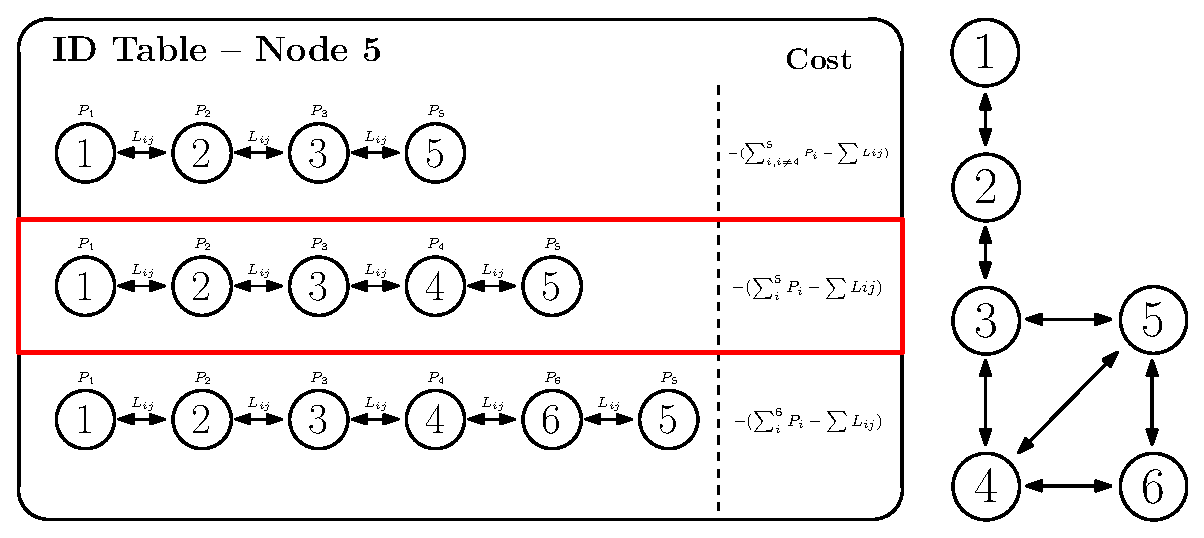
\includegraphics[width=0.9\textwidth]{fig/05_den2ne/den2ne_09.eps}
    \caption{Selección de ID basada en el criterio de balance de potencia con pérdidas.}
    \label{fig:den2ne_09}
\end{figure}

\subsubsection{Criterio 6 - Balance de potencia ponderado}

El sexto y último criterio representa una implementación alternativa, mediante ponderaciones, de las ideas presentadas en los dos criterios anteriores~\cite{Schneider17,Ma97}. Mientras que el criterio 5 penaliza la ruta en función de la longitud y otros parámetros de pérdidas, el criterio 6 normaliza la capacidad de potencia de la ruta en función del número de nodos atravesados. Este criterio pone de manifiesto directamente el efecto negativo que puede tener el criterio 4, que busca el mayor balance de potencia, ya que eventualmente podría favorecer rutas más largas hacia la raíz. Por lo tanto, el criterio 5 reajusta este cálculo considerando también las pérdidas potenciales, y el criterio 6 proporciona un balance de potencia ponderado, de modo que se tenga en cuenta tanto la capacidad como el número de saltos en la ruta. Este criterio puede resultar particularmente útil cuando no se dispone de una representación clara de las pérdidas de los enlaces. La fórmula resultante se representa en la Ecuación~\ref{eq:criterionCost06}.  
 

\begin{equation}\label{eq:criterionCost06}
      Cost_{ID}  \: = \: -(\frac{1}{M}\sum_{i}^{N_{ID}} P_{i}), \: \: M = \frac{1}{(lenght(ID) \: - \: 1)}
\end{equation}
\vspace{0.2cm}

Considerando el ejemplo de la Figura~\ref{fig:den2ne_10}, el $ID_{activa}$ corresponde a la ruta \texttt{1.2.3.4.5}, que tiene un menor número de nodos que la seleccionada en el criterio 4, como era de esperar, pero presenta la mejor relación $\frac{recursos}{saltos}$ entre todas las rutas. Esta ruta cumple la condición representada en la Ecuación~\ref{eq:criterionCost06_b}.

\begin{equation}\label{eq:criterionCost06_b}
           \left \langle ID_{2} = ID_{activa} \right \rangle \Leftrightarrow  
           \left\{\begin{matrix}
           [\frac{1}{4}\sum_{i}^{5} P_{i} > \frac{1}{3}\sum_{i,i\neq4}^{5} P_{i}] \\
       \\
       \wedge \\ 
       \\ [\frac{1}{4}\sum_{i}^{5} P_{i} > \frac{1}{5}\sum_{i}^{6} P_{i}]
           \end{matrix}\right.
\end{equation}
\vspace{0.2cm}

\begin{figure}[ht!]
    \centering
    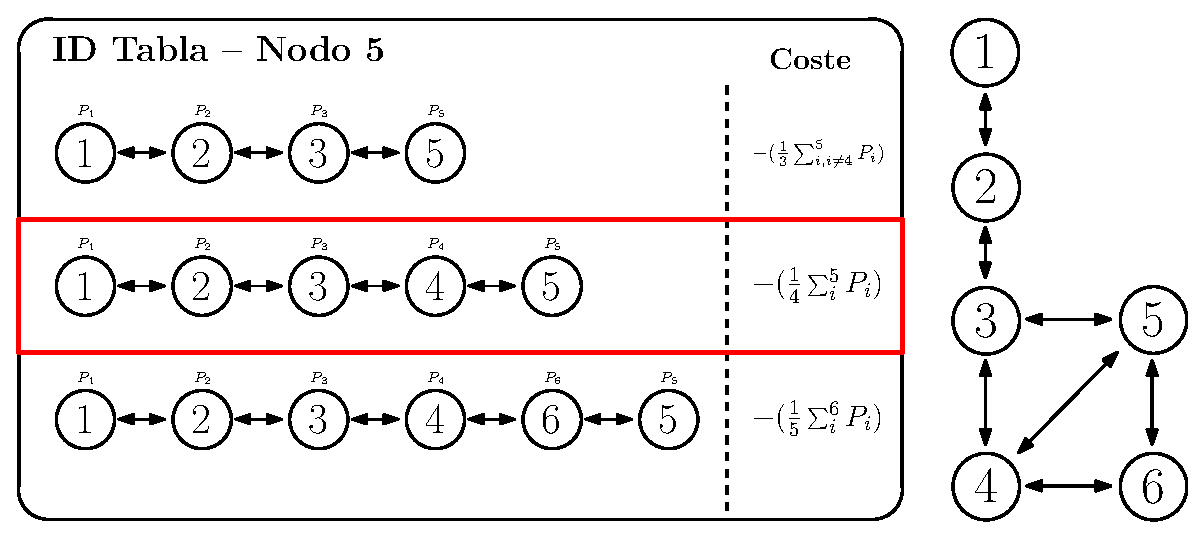
\includegraphics[width=0.9\textwidth]{fig/05_den2ne/den2ne_10.eps}
    \caption{Selección de ID basada en el criterio de balance de potencia ponderado.}
    \label{fig:den2ne_10}
\end{figure}


\subsection{Fase 3 - Balance global}
\label{subsec:fase3}

Una vez que las etiquetas se asignan a lo largo de toda la topología, se aplica un criterio determinado y cada nodo tiene un $ID_{activa}$, puede comenzar el procedimiento para equilibrar los recursos disponibles. El objetivo del algoritmo es alcanzar un estado de balance global trasladando recursos desde los nodos más alejados, hacia la raíz. Este movimiento se implementa de manera local, pero siguiendo un orden específico basado en el $ID_{activa}$ de cada nodo, lo que finalmente produce un equilibrio general de los recursos para todos los nodos de la topología. \\
\\
Para proceder, dado que el algoritmo es centralizado, es posible recopilar el $ID_{activa}$ de cada nodo y ordenarlos en función de su longitud. Cuanto más largo sea el $ID_{activa}$, más alejado estará el nodo, desde un punto de vista lógico, de la raíz\footnote{Es importante destacar el adverbio \textit{lógicamente} en este contexto, ya que el nodo podría estar físicamente más cerca, pero el $ID_{activa}$ seleccionado puede proporcionar una vista lógica diferente.}. Por lo tanto, el algoritmo comienza equilibrando la carga desde el $ID_{activa}$ más largo, que está asociado a un nodo específico de la red. En caso de que dos o más $ID_{activa}$ tengan la misma longitud, se seleccionará uno de ellos de manera aleatoria. Una vez que los nodos se ordenan en función de su $ID_{activa}$, el algoritmo visita cada nodo una sola vez para equilibrar el recurso con su nodo predecesor en la lista ordenada representada por el $ID_{activa}$. Considerando la terminología explicada en la sección~\ref{subsec:terminologiaDEN2NE}, las demandas se expresarán como un valor negativo y las ofertas como un valor positivo, siendo el objetivo dejar a cada nodo en un estado neutro (en este caso, sin demanda ni oferta implica un valor cero) y transferir la demanda u oferta restante al siguiente vecino de la lista. Este proceso se repite para cada nodo hasta llegar al último nodo de la lista (que corresponde al nodo con el $ID_{activa}$ más corto, es decir, el nodo raíz). En consecuencia, la raíz obtiene la oferta o demanda restante de toda la red, es decir, el balance global. Posteriormente, el nodo raíz, como nodo pasarela hacia el núcleo de la red, puede decidir por sí mismo qué hacer con dicha oferta o demanda sobrante. \\
\\
Para ejemplificar el procedimiento descrito, se presenta la Figura~\ref{fig:den2ne_11}, la cual, representa la topología de la red de ejemplo utilizada para explicar el algoritmo hasta el momento, en la cual el $ID_{activa}$ más largo es el asociado al nodo 5 (\texttt{1.2.3.4.6.5}). En consecuencia, la Figura~\ref{fig:den2ne_11} muestra la lista ordenada, donde el primer nodo a comprobar es el nodo 5, mientras que el último es el nodo 1. Para simplificar, en la figura solo se representan los $ID_{activa}$ de los tres primeros nodos que serán visitados (5, 6 y 4). En este escenario, el nodo 5 tiene una oferta de $3.1$, el nodo 6 tiene una demanda de $-1$, y el nodo 4 una oferta de $0.5$. Como el algoritmo comienza en el nodo 5, su estado se fijará en cero, y su oferta se transferirá al siguiente vecino en la lista, el nodo 6, que ahora actualizará sus recursos a $-1+3.1 \:= \:2.1$, tal como se muestra en la Figura~\ref{fig:den2ne_12}. Posteriormente, el siguiente nodo a procesar será el nodo 6 (\texttt{1.2.3.4.6}), que también se fijará en cero y su oferta o demanda se transferirá al siguiente nodo, de modo que el nodo 4 pase a tener $0.5+2.1 \: = \: 2.6$, como se ilustra en la Figura~\ref{fig:den2ne_13}. El algoritmo \gls{d2e} continúa procesando todos los nodos hasta llegar finalmente al nodo raíz, de manera que todos los nodos quedan equilibrados y el nodo raíz obtiene un valor global de oferta/demanda de la red.

% \begin{figure}[ht!]
%     \centering
%     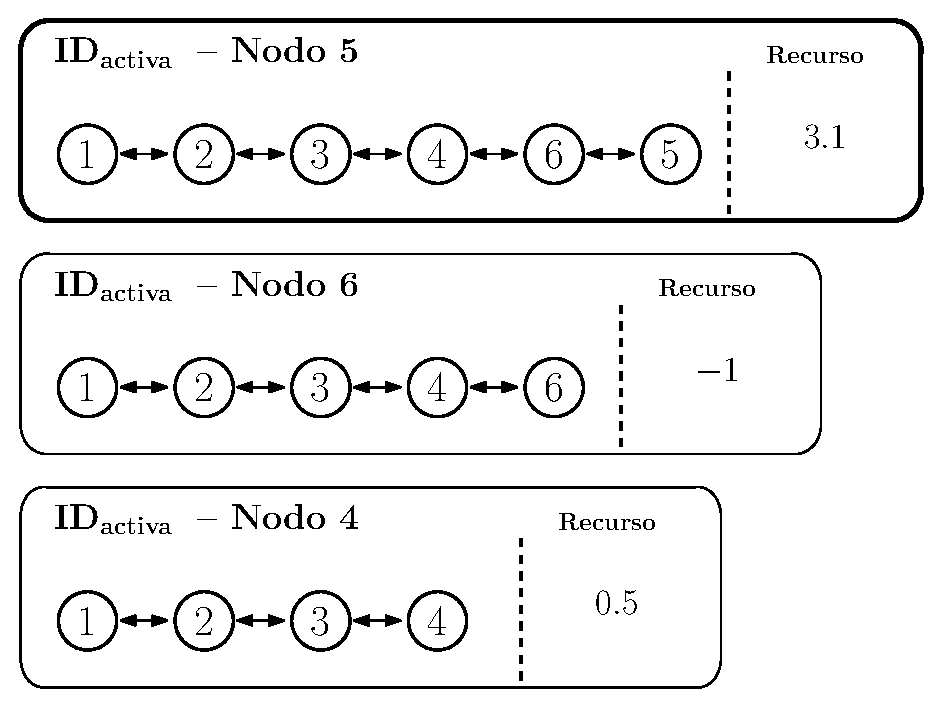
\includegraphics[width=0.55\textwidth]{fig/05_den2ne/den2ne_11.eps}
%     \caption{Ejemplo del procedimiento de balance global - Paso 1.}
%     \label{fig:den2ne_11}
% \end{figure}

% \begin{figure}[ht!]
%     \centering
%     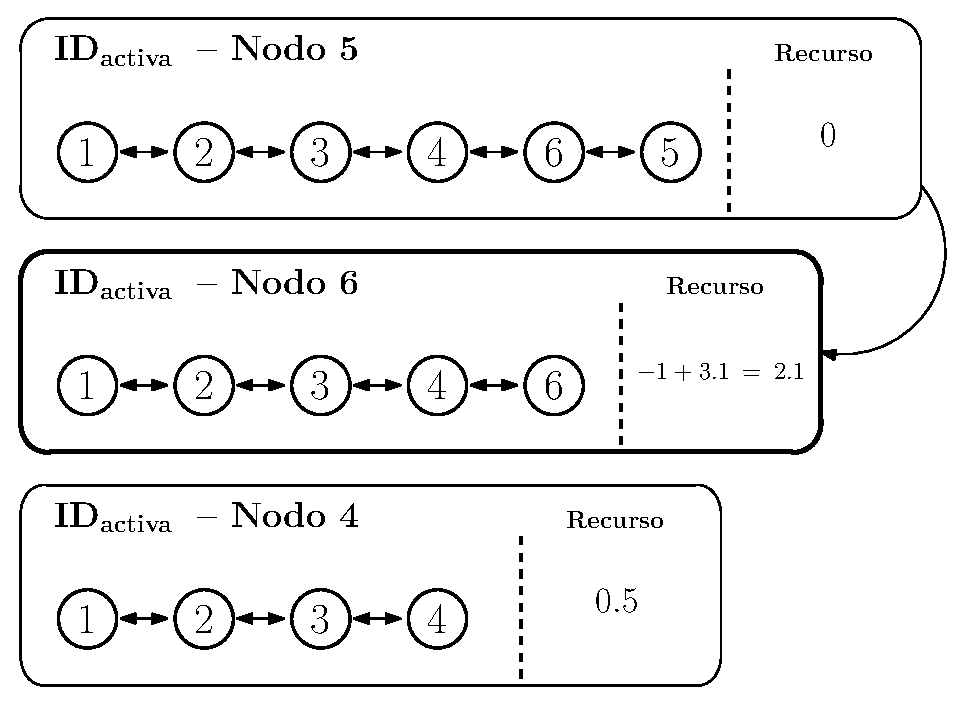
\includegraphics[width=0.55\textwidth]{fig/05_den2ne/den2ne_12.eps}
%     \caption{Ejemplo del procedimiento de balance global - Paso 2.}
%     \label{fig:den2ne_12}
% \end{figure}

% \begin{figure}[ht!]
%     \centering
%     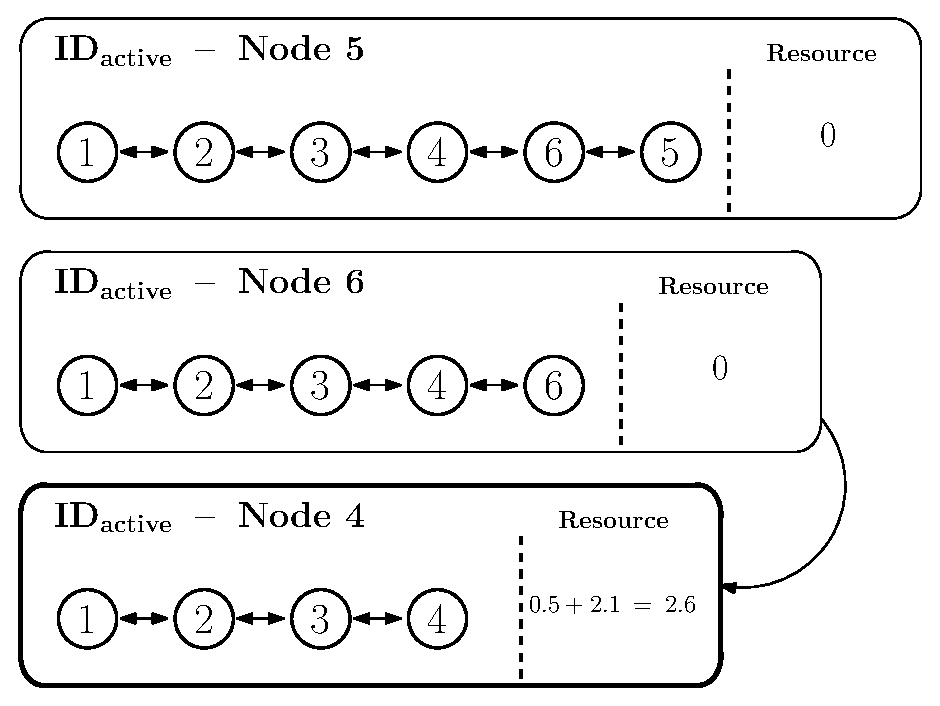
\includegraphics[width=0.55\textwidth]{fig/05_den2ne/den2ne_13.eps}
%     \caption{Ejemplo del procedimiento de balance global - Paso 3.}
%     \label{fig:den2ne_13}
% \end{figure}
\begin{figure}[H]
    \centering
    
    \begin{subfigure}{0.55\textwidth}
        \centering
        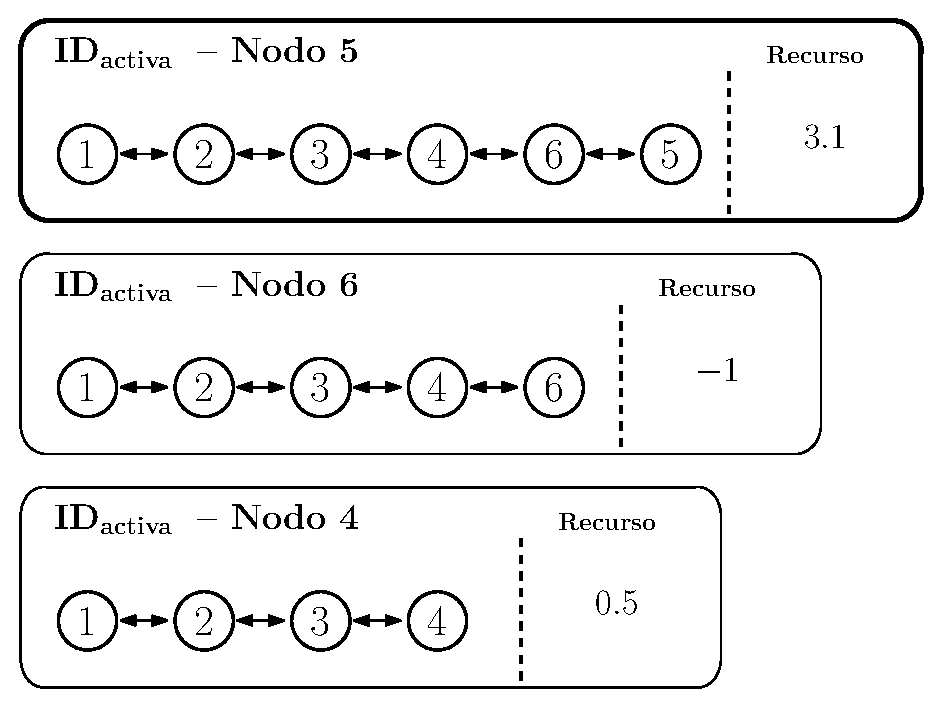
\includegraphics[width=\linewidth]{fig/05_den2ne/den2ne_11.eps}
        \caption{Paso 1.}
        \label{fig:den2ne_11}
    \end{subfigure}
    
    \vspace{0.3cm}
    
    \begin{subfigure}{0.55\textwidth}
        \centering
        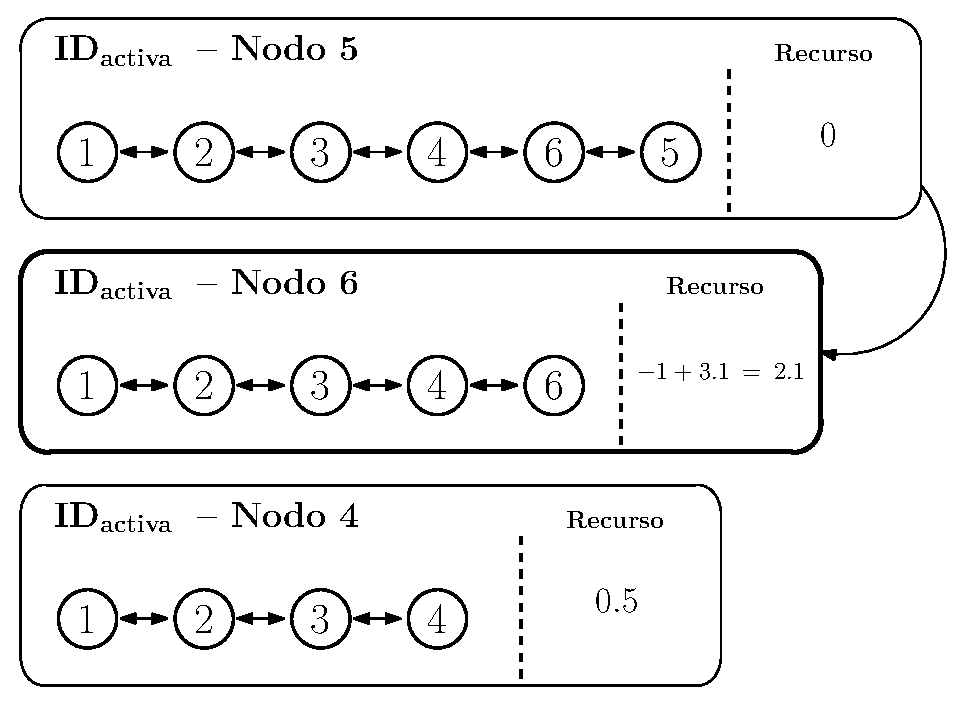
\includegraphics[width=\linewidth]{fig/05_den2ne/den2ne_12.eps}
        \caption{Paso 2.}
        \label{fig:den2ne_12}
    \end{subfigure}
    
    \vspace{0.3cm}
    
    \begin{subfigure}{0.55\textwidth}
        \centering
        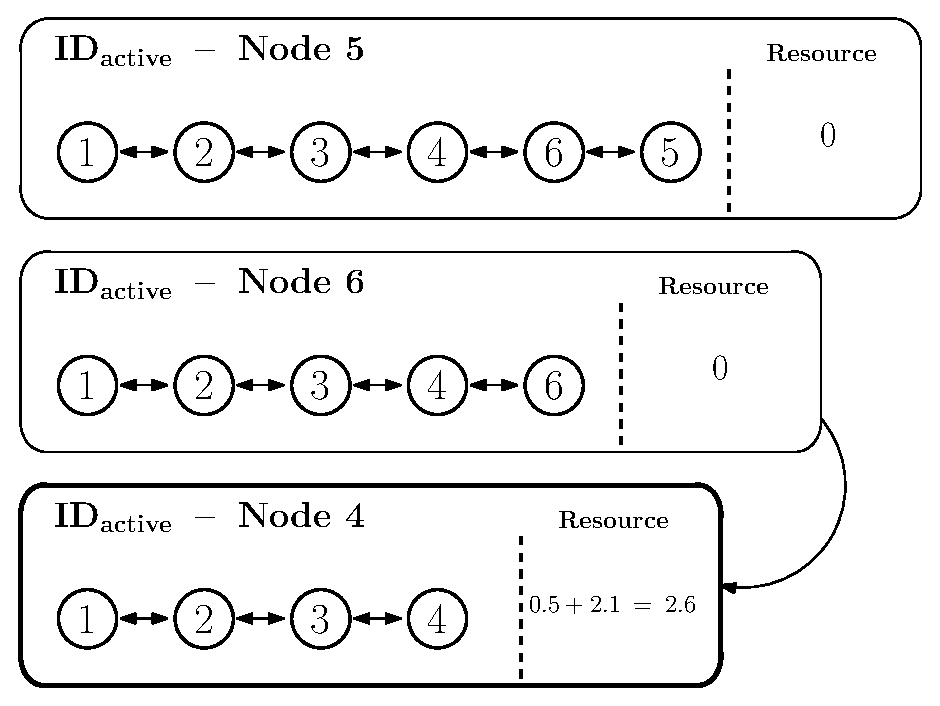
\includegraphics[width=\linewidth]{fig/05_den2ne/den2ne_13.eps}
        \caption{Paso 3.}
        \label{fig:den2ne_13}
    \end{subfigure}
    
    \caption{Ejemplo del procedimiento de balance global.}
    \label{fig:den2ne_balance}
\end{figure}


El procedimiento anterior se resume en el Algoritmo~\ref{alg:globalbalance}. Como se puede observar, las entradas del algoritmo son: (1) el grafo $G(\mathcal{N}, \mathcal{L})$, que es el conjunto de nodos de la topología ($\mathcal{N}$) y enlaces ($\mathcal{L}$), y (2) el $scenario\_type$, que puede ser uno de los siguientes cuatro (definidos únicamente como referencia para representar y, posteriormente, evaluar, distintos casos de uso): 


\begin{itemize}

    \item \textbf{Escenario ideal}: Representa un escenario en el que no existe pérdida de recursos durante la transmisión cuando el recurso ($r_{i}$) se envía de un nodo $i$ a otro $j$ ($i,j \in \mathcal{N} \: \:\forall \:\: i \neq j$) a través de un enlace sin pérdidas, es decir, $L_{ij} \: = 0$. En consecuencia, para cualquier transmisión de recursos $i \rightarrow j$, en la que el estado inicial es $\{i=r_{i},\: j=r_{j}\}$, los recursos resultantes tras la transmisión son $\{i' = 0,\: j' = r_{i}+r_{j}\}$.
    
    
    \item \textbf{Escenario con pérdidas}: Implica la existencia de pérdidas durante la transmisión de recursos, es decir, $L \: \neq \varnothing$. En consecuencia, para cualquier transmisión de recursos $i \rightarrow j$, en la que el estado inicial es $\{i=r_{i},\: j=r_{j}\}$, los recursos resultantes tras la transmisión son $\{i' = 0,\: j' = r_{i}+r_{j}-L_{ij}\}$. El modelo de pérdidas que se empleará está descrito en \cite{Schneider17}, utilizando las pérdidas de transmisión definidas en la Ecuación \ref{eq:criterionCost04_b}.
    
    
    \item \textbf{Escenario con capacidad de enlace restringida}: Hasta ahora, los enlaces no tenían ninguna limitación particular al transmitir un recurso, pero si el enlace está restringido a ciertos valores de transmisión, el recurso no se reenviará oportunamente y el excedente será descartado (al menos, de forma lógica para el algoritmo, incluso si el exceso de recurso permanece en su origen). Más específicamente, si la capacidad del enlace es $C_{ij}$, con $C \: \neq \varnothing$, y $r_{i} \geq C_{ij}$, entonces la transmisión de recursos asociada $i \rightarrow j$ con estado inicial $\{i=r_{i},\: j=r_{j}\}$ resultará en el estado final $\{i' = 0,\: j' = \: C_{ij}+r_{j}\}$. El modelo de las capacidades de los enlaces empleados está descrito en \cite{Schneider17}, donde se especifica que la capacidad máxima de cada enlace es $C_{max} \: = I_{max} \: \times \: V_{d}$.
    
    
    \item \textbf{Escenario con pérdidas y capacidad de enlace restringida}: Este último tipo combina los dos anteriores, es decir, $L \: \neq \varnothing$ y $C \: \neq \varnothing$. En consecuencia, para cualquier transmisión de recursos $i \rightarrow j$, en la que el estado inicial es $\{i=r_{i},\: j=r_{j}\}$, los recursos resultantes tras la transmisión son $\{i' = 0,\: j' = r_{i}+r_{j}-L_{ij}\}$ en caso de que $r_{i} \leq C_{ij}$, y $\{i' = 0,\: j' = C_{ij}+r_{j}-L_{ij}\}$ en caso de que $r_{i} \geq C_{ij}$.  
 
\end{itemize}

Con respecto a las salidas del Algoritmo~\ref{alg:globalbalance}, $total\_balance\_ideal$ proporciona el balance global de la topología (que corresponde a la carga final en la raíz, ya que esta permanece como el último nodo y conserva la diferencia de todas las transferencias de recursos; de ahí que $total\_balance \: = \: root.load$), mientras que $abs\_flux$ proporciona un valor absoluto de los intercambios de recursos a lo largo de la red (para cualquier intercambio se considera su valor absoluto, ya que el signo negativo o positivo solo indica la dirección, pero el movimiento de recursos ocurre en cualquier caso). \\
\\
Por lo tanto, $total\_balance$ expresa si la red presenta una demanda o un exceso global de recursos, mientras que $abs\_flux$ representa el cantidad de recursos distribuidos. 

\begin{algorithm}[ht!]
\caption{Proceso de balance global}\label{alg:globalbalance}
\SetKwInOut{Input}{input}
\SetKwInOut{Output}{output}
\Input{$\: G(\mathcal{N}, \mathcal{L}),\: scenario\_type$}
\Output{$\: total\_balance, \: abs\_flux$}
\vspace{0.2cm}
$\textup{init}\: global\_ids, abs\_flux$\;
$\textup{sort}\: global\_ids$\;
\vspace{0.1cm}
\While{$length(global\_ids) > 1$}{
\vspace{0.1cm}
    $origin \: = \: \mathcal{N}(global\_ids[0])$\;
    $destination \: = \: \textup{get next hop from} \:origin$\;
\vspace{0.1cm}  

  \eIf{$origin.load \: > 0$}{
    $\textup{setLinkDirection} \: \mathcal{L}(origin, \: destination) \: \textup{to down}$\;

  }{
    $\textup{setLinkDirection} \: \mathcal{L}(origin, \: destination) \: \textup{to up}$\;
  }


    \Switch{$scenario\_type$}{
        \Case{$ideal$}{ 
                $destination.load \: = destination.load \: + \: origin.load$\;
                $abs\_flux \: = abs\_flux  \: + \:\left |  origin.load \right |$\;
        }
        \Case{$lossy$}{
              $destination.load \: = destination.load \: + \: origin.load \: - \: \textup{losses}$\;
              $abs\_flux \: = abs\_flux  \: + \:\left |  origin.load  \: - \: \textup{losses}\right |$\;
        
        }
        \Case{$capacity$}{
            \eIf{$origin.load \geq capacity$}{
                $destination.load \: = destination.load \: + \: capacity$\;
                $abs\_flux \: = abs\_flux  \: + \:\left |  capacity \right |$\;
            }{
                $destination.load \: = destination.load \: + \: origin.load$\;
                $abs\_flux \: = abs\_flux  \: + \:\left |  origin.load \right |$\;
            }
        }
        \Other{
            \eIf{$origin.load \geq capacity$}{
                $destination.load \: = destination.load \: + \: capacity \: - \: \textup{losses}$\;
                $abs\_flux \: = abs\_flux  \: + \:\left |  capacity \: - \: \textup{losses} \right |$\;
            }{
                $destination.load \: = destination.load \: + \: origin.load \: - \: \textup{losses}$\;
                $abs\_flux \: = abs\_flux  \: + \:\left |  origin.load \: - \: \textup{losses} \right |$\;
            }
        }
    }

    %\vspace{0.1cm}
  $origin.load \: = \: \varnothing$\;
  $\textup{pop}\: global\_ids[0]$\;
  
}
%\vspace{0.1cm}
\Return{$root.load, abs\_flux$}
\end{algorithm}

Concretamente, $total\_balance$ podría ser igual o cercano a cero, lo cual significa que la red no tiene una demanda específica de recursos, pero $abs\_flux$ podría indicar un valor elevado, lo que evidencia que, para alcanzar un balance global, se requiere un alto número de intercambios. De hecho, $total\_balance$ simplemente ilustra la naturaleza del escenario (es decir, cantidad de ofertas frente a demandas), mientras que $abs\_flux$ constituye realmente un indicador de la eficacia del algoritmo, ya que cuanto menor sea su valor, menor será el coste para balancear óptimamente la carga de recursos en la topología.\\
\\
Como se puede observar, el Algoritmo~\ref{alg:globalbalance} es lineal (complejidad $\mathcal{O}(n)$), ya que los nodos de la red son visitados una sola vez considerando la etiqueta o identificador seleccionado en la segunda fase del algoritmo, lo cual queda representado por el único bucle ($while$) del mismo. Finalmente, cabe destacar que el algoritmo \gls{d2e} se ejecuta en base a una instantánea específica de la red. Si la red se actualiza debido a la movilidad de nodos, o a la modificación de ofertas y demandas, el algoritmo puede ejecutarse de nuevo, en cualquier momento, para redistribuir los nuevos recursos.

\section{Entorno de evaluación}
\label{sec:den2ne_setup}
La implementación y configuración de la evaluación están basadas en Python 3.8\footnote{\url{https://peps.python.org/pep-0569/}}. Más específicamente, la evaluación se divide en dos etapas:

\begin{enumerate}
    \item Un generador de topologías aleatorias para probar exhaustivamente \gls{d2e}, que aprovecha el entorno \gls{brite}~\cite{brite}, como se muestra en la Figura~\ref{fig:den2ne_14} (el cual traduce los archivos \texttt{*.brite} en archivos \texttt{*.csv} para los nodos y enlaces de la topología, utilizados como entrada en nuestro algoritmo).
   
    \item La ejecución del algoritmo, desarrollado como un script centralizado, que importa todas las topologías generadas, una por una, utilizando semillas y diferentes parámetros de \gls{d2e} para su comparación. 
\end{enumerate}

\begin{figure}[ht!]
    \centering
    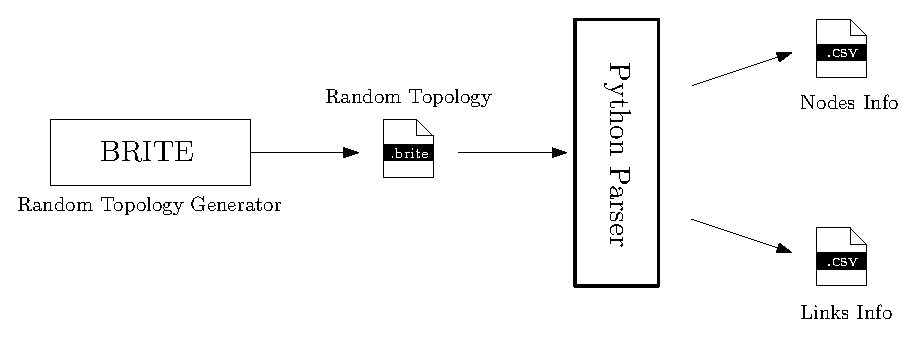
\includegraphics[width=0.7\textwidth]{fig/05_den2ne/den2ne_14.eps}
    \caption{Generador de topologías para DEN2NE basado en BRITE.}
    \label{fig:den2ne_14}
\end{figure}

Nuestro objetivo es proporcionar un análisis exhaustivo del algoritmo \gls{d2e}, abarcando la mayor cantidad posible de tipos de escenarios. De hecho, los grafos proporcionados por \gls{brite} se basan en topologías aleatorias Waxman~\cite{waxman1988routing} y Barabási-Albert~\cite{barabasi1999emergence}, las cuales se emplean para modelar una amplia gama de sistemas de interconexión, desde redes de computación, a redes de comunicaciones, y hasta redes sociales. La red aleatoria Waxman se fundamenta en un modelo probabilístico para la generación aleatoria de una red, mientras que la red Barabási-Albert se enmarca dentro de la categoría de redes \textit{scale-free} (también conocidas como redes \textit{hub-and-spoke}), en las cuales ciertos nodos presentan un número de conexiones significativamente mayor que el resto. Una vista simplificada de ambos modelos se muestra en la Figura~\ref{fig:den2ne_15}.

\begin{figure}[ht!]
    \centering
    \begin{subfigure}[t]{0.45\textwidth}
        \centering
        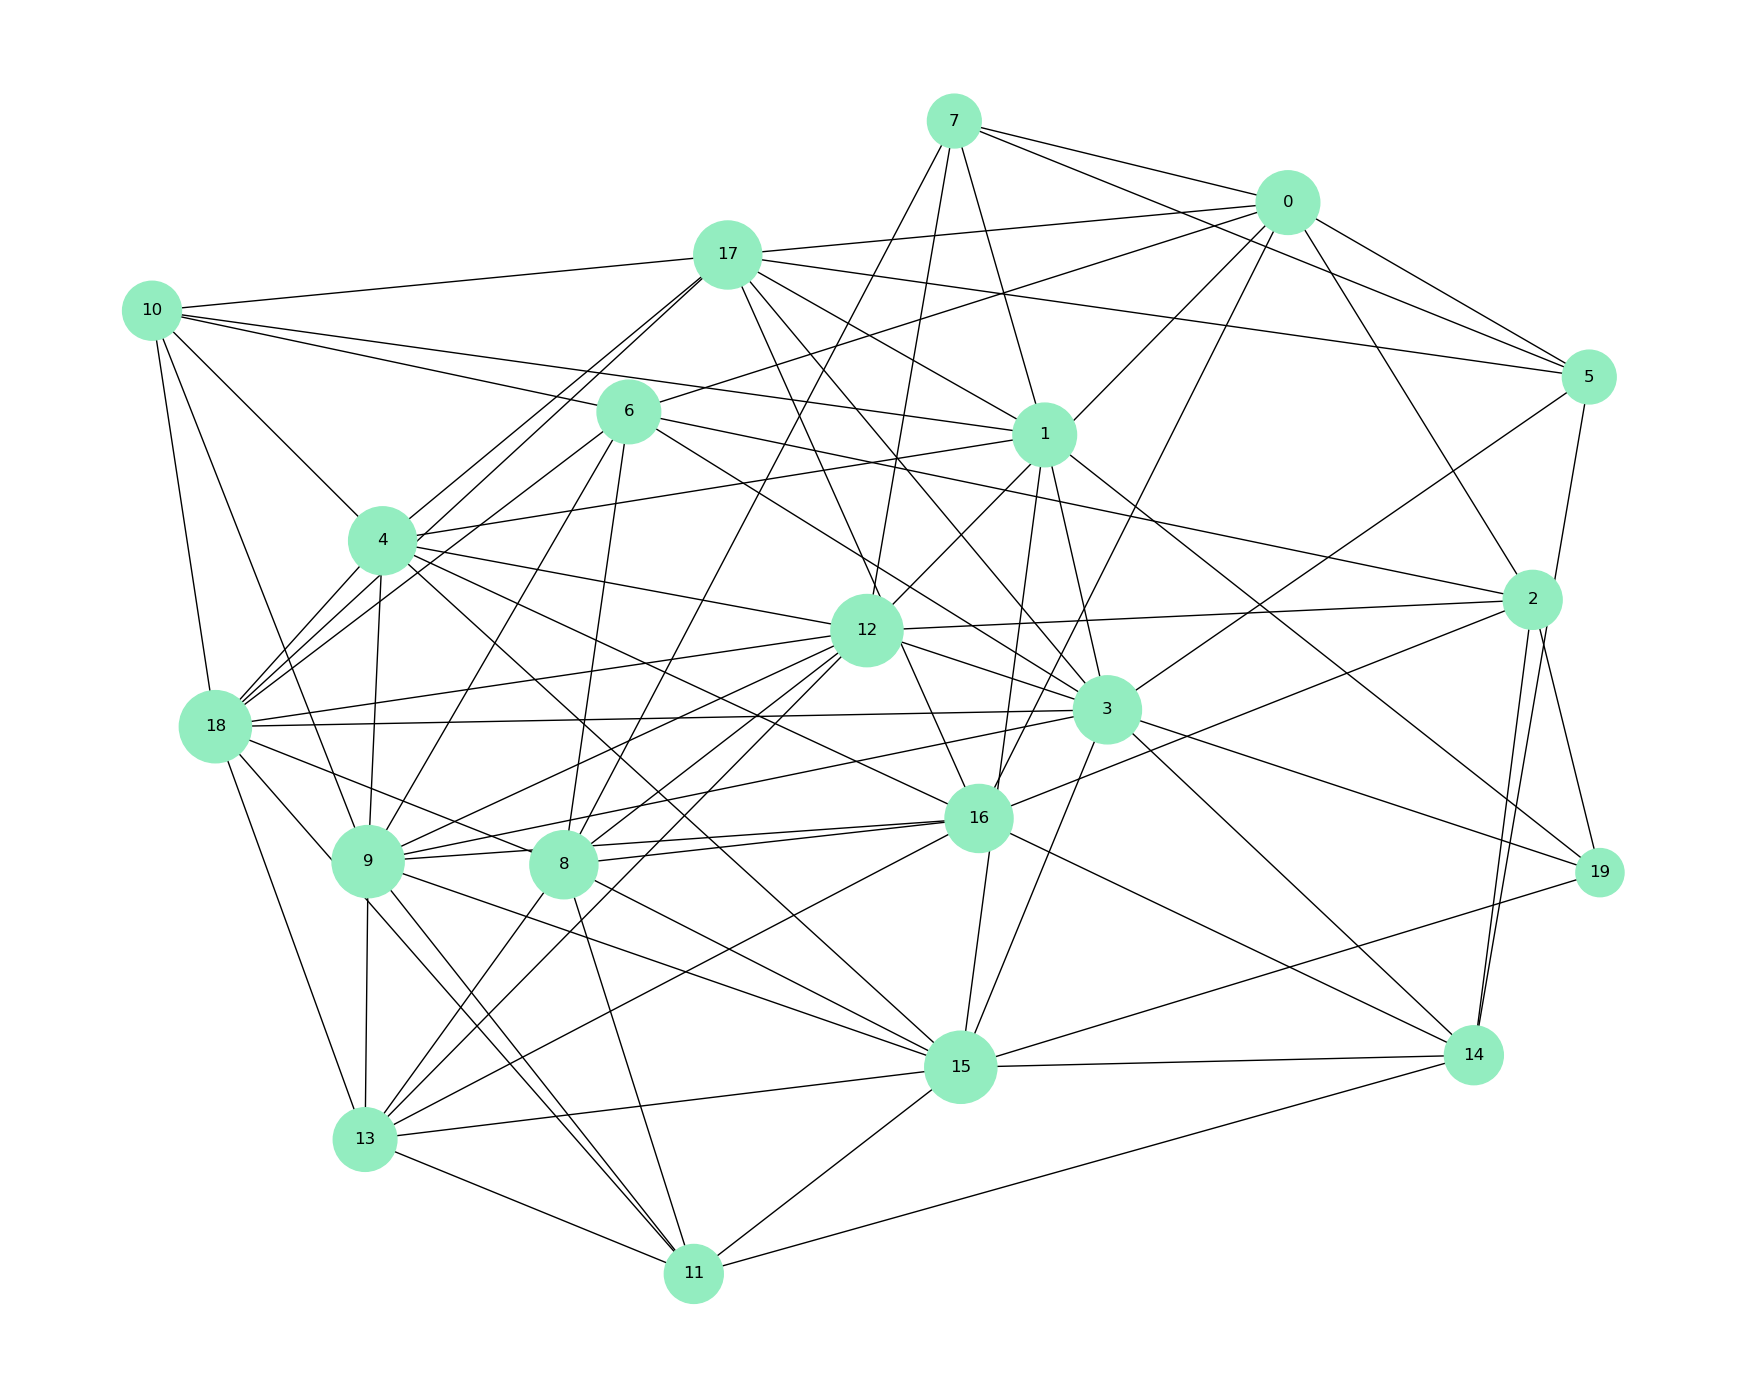
\includegraphics[width=\linewidth]{fig/05_den2ne/den2ne_15a.png}
        \caption{Topología Waxman}
        \label{fig:waxman}
    \end{subfigure}
    \hfill
    \begin{subfigure}[t]{0.45\textwidth}
        \centering
        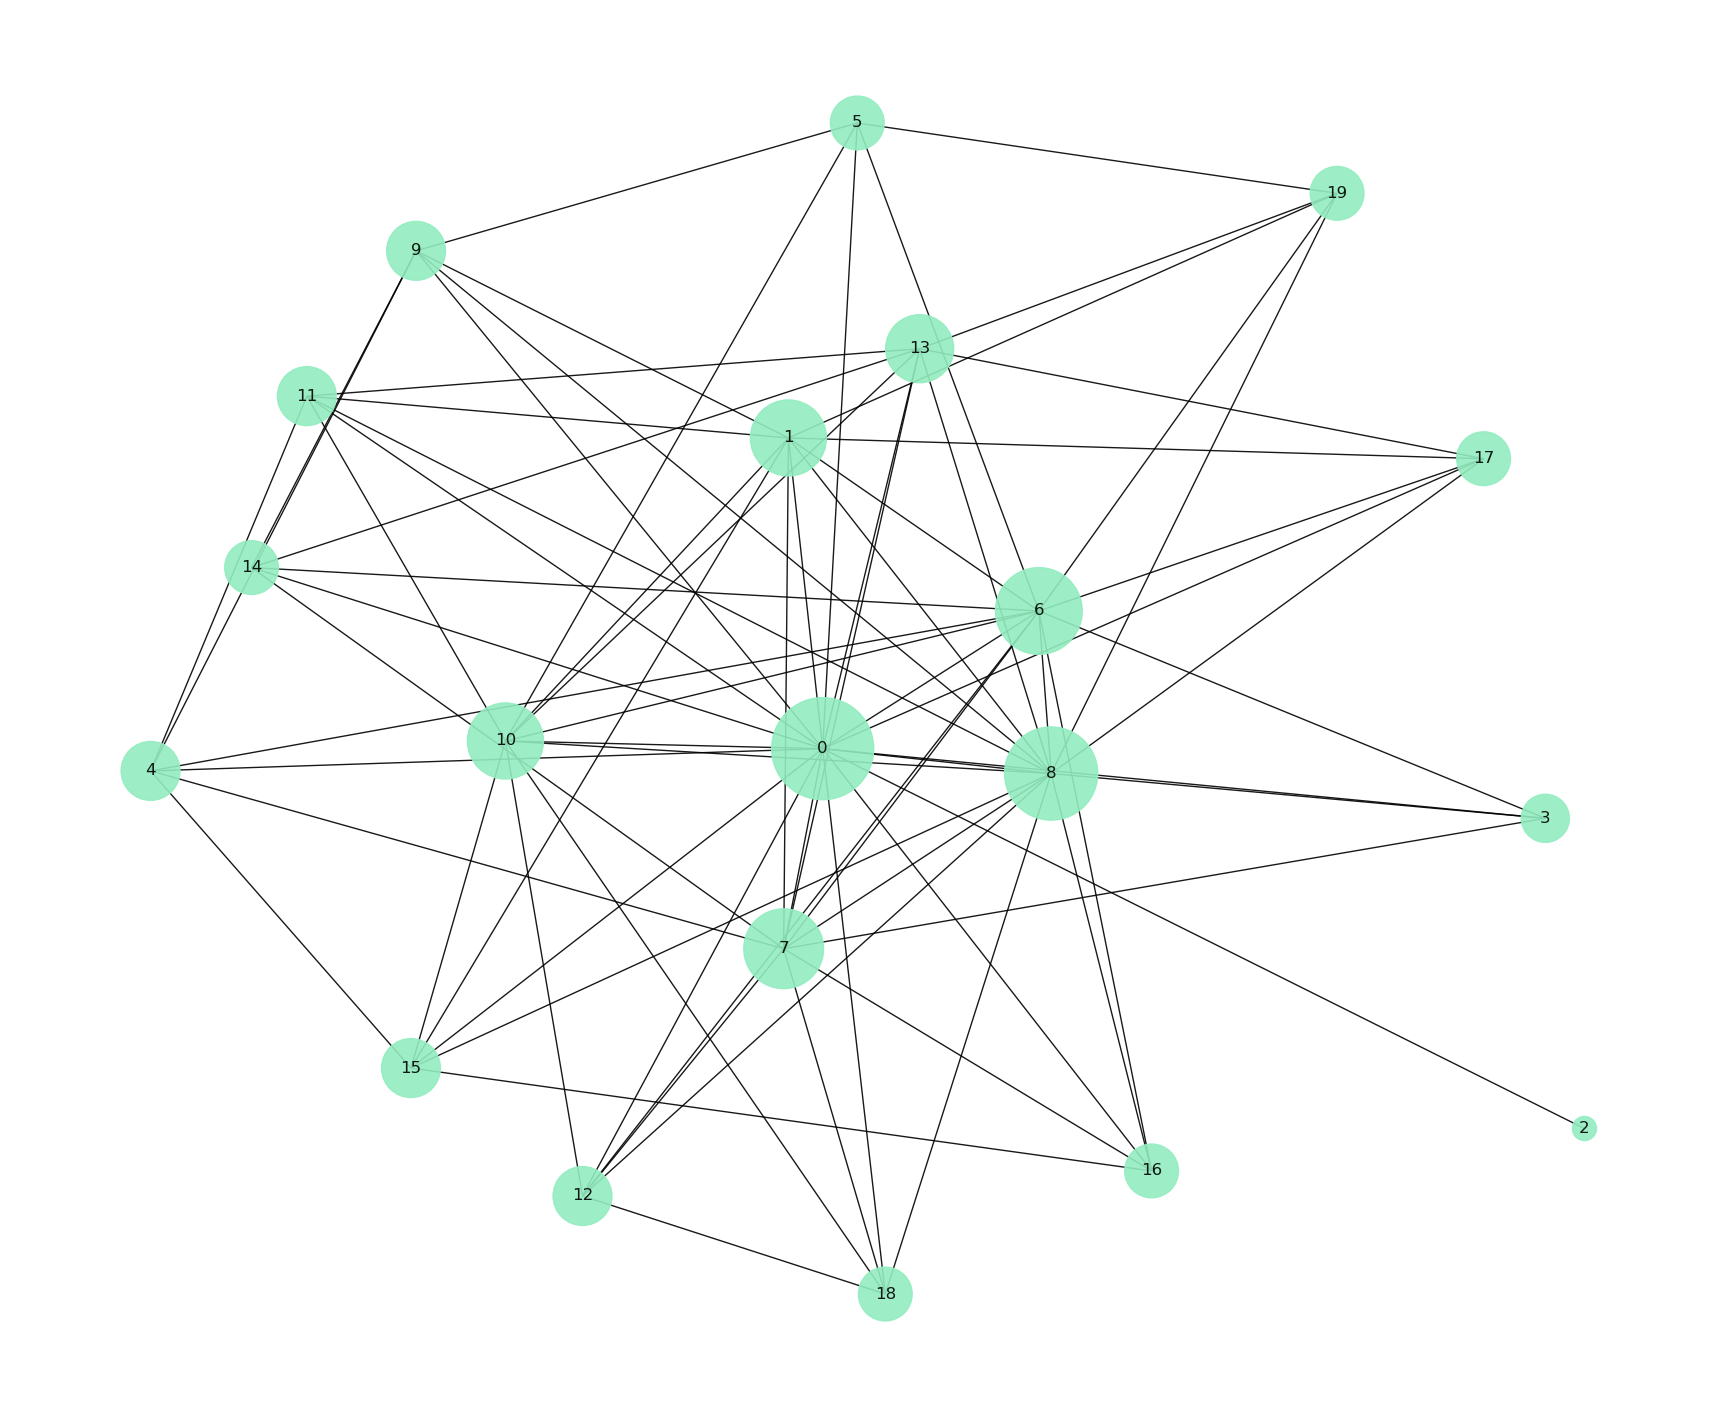
\includegraphics[width=\linewidth]{fig/05_den2ne/den2ne_15b.png}
        \caption{Topología Barabási-Albert}
        \label{fig:barabasi}
    \end{subfigure}
    \caption{Topologías aleatorias empleadas en el estudio de DEN2NE.}
    \label{fig:den2ne_15}
\end{figure}

En lo que respecta a los parámetros de generación de topologías, estos se resumen en la Tabla~\ref{tab:topologyParams}, la cual incluye: tipo de topología (uno de los dos tipos mencionados anteriormente), número de nodos (de 10 a 200 nodos en intervalos de 10 nodos), grado de conectividad (número promedio de enlaces por nodo, de 4 a 6, en intervalos de 2 enlaces) y una semilla de topología aleatoria (para obtener 10 topologías aleatorias de cada tipo). De acuerdo con estos parámetros, el número total de topologías evaluadas fue de 1200, tal y como se indica en la Ecuación~\ref{eq:numtopos}.


\begin{table}[ht!]
\centering
\begin{tabular}{|l|c|}
\hline
\multicolumn{1}{|c|}{\textbf{Atributos}} & \textbf{Valores} \\ \hline
Tipo de topología & {[}"\texttt{waxman}", "\texttt{barabasi-albert}"{]} \\ \hline
Número de nodos & {[}\texttt{10:10:200}{]} \\ \hline
Grado de conectividad & {[}\texttt{4:2:6}{]} \\ \hline
Semillas de las topologías aleatorias & {[}\texttt{1:1:10}{]} \\ \hline
\end{tabular}
\vspace{0.2cm}
\caption{Parámetros de generación de las topologías aleatorias.}
\label{tab:topologyParams}
\end{table}

\begin{equation}\label{eq:numtopos}
\begin{split}    
    \left \langle N_{topos} \right \rangle  \: & = { \: N_{tipo} \: \times \: N_{nodos} \: \times \:  N_{grado} \: \times \: N_{semilla}} \\
    & = 2 \times 20 \times 3 \times 10 \: = \: 1200 \: \: topos
\end{split}
\end{equation}
\vspace{0.2cm}

La evaluación realizada tiene como objetivo comparar el comportamiento de los 6 criterios descritos en la Sección~\ref{subsec:fase2} en cuatro tipos de escenarios de red (ideal, con pérdidas, con capacidad de enlace restringida y con capacidad de enlace restringida y pérdidas). Adicionalmente, el banco de pruebas debía asignar una oferta o demanda inicial de recursos a cada nodo de la topología. Esta asignación de recursos fue agnóstica (no se asocia ninguna unidad o métrica en particular) y podía estar limitada a un valor total determinado (fijado en 250, asumiendo al menos 1 unidad de recurso por nodo en promedio en las topologías más grandes) o no estarlo (sin un valor máximo establecido). La limitación en la asignación de recursos se definió con el fin de depurar la implementación y el comportamiento del algoritmo en los escenarios más complejos. En cualquier caso, tanto en la versión limitada como en la no limitada, la carga asignada a cada nodo siguió una distribución uniforme, como se ilustra en la Figura~\ref{fig:den2ne_16}.

\begin{figure}[ht!]
    \centering
    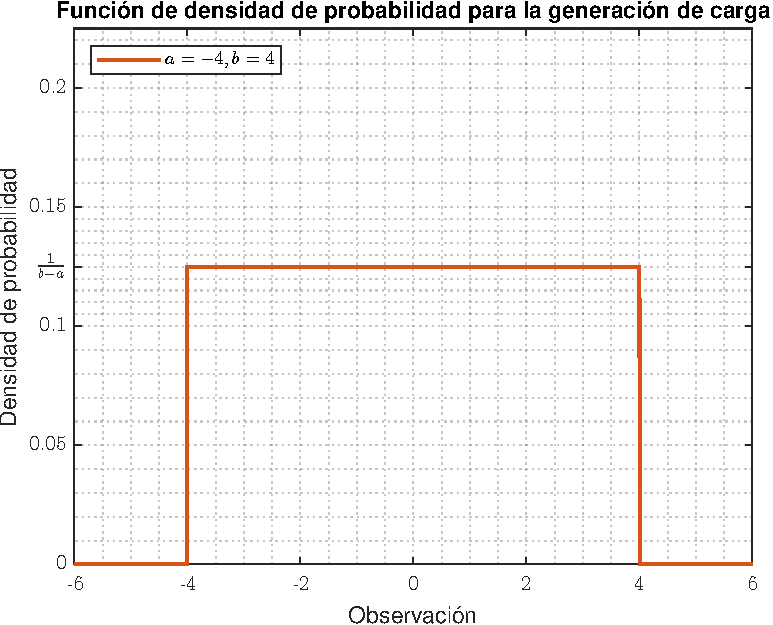
\includegraphics[width=0.7\textwidth]{fig/05_den2ne/den2ne_16.pdf}
    \caption{Función de densidad de probabilidad para la generación de cargas aleatorias en cada topología.}
    \label{fig:den2ne_16}
\end{figure}

Finalmente, para validar nuestros resultados, cada escenario se repitió 10 veces utilizando diferentes semillas para la generación aleatoria de recursos. Estas semillas solo modificaban la ubicación de la raíz y la asignación de recursos, mientras que el resto del escenario se mantenía igual, con el fin de demostrar exhaustivamente la validez de los resultados obtenidos. Todos estos parámetros se resumen en la Tabla~\ref{tab:testparams}. Por lo tanto, el número total de simulaciones de nuestro estudio es de 576000, tal y como se indica en la Ecuación~\ref{eq:numsim}.


\begin{equation}\label{eq:numsim}
\begin{aligned}
    \left \langle N_{simulaciones} \right \rangle  \: & = \: { N_{topos} \: \times \: N_{criterios} \: \times \:  N_{escenarios} \: \times \: N_{LR} \: \times \: N_{semilla}} \\ \: & = 1200 \times 6 \times 4 \times 2 \times 10 \\
    \: & = \: 576000 \: \: simulaciones
\end{aligned}    
\end{equation}
\vspace{0.2cm}

\begin{table}[ht!]
\centering
\begin{tabular}{|l|c|}
\hline
\multicolumn{1}{|c|}{\textbf{Atributo}} & \textbf{Valores} \\ \hline
Criterios & {[}\texttt{1:1:6}{]} \\ \hline
Tipo de escenario & {[}\texttt{1:1:4}{]} \\ \hline
Limitación de recursos & {[}\texttt{0,1}{]} \\ \hline
Semilla de ejecución aleatoria & {[}\texttt{1:1:10}{]} \\ \hline
\end{tabular}
\vspace{0.2cm}
\caption{Parámetros para la ejecución de pruebas.}
\label{tab:testparams}
\end{table}

\section{Resultados y evaluación del algoritmo}

Considerando la implementación y el entorno de evaluación presentados en la Sección~\ref{sec:den2ne_setup}, en esta sección se exponen los resultados obtenidos a partir de las simulaciones descritas. Para evaluar el comportamiento de \gls{d2e}, se midieron tres métricas diferentes: la primera en relación con el balance de recursos (que corresponde a una de las salidas del algoritmo \gls{d2e}, tal y como se describió previamente en el Algoritmo~\ref{alg:globalbalance}), y las otras dos en relación con el tiempo de ejecución, tanto para la asignación de etiquetas como para el balance de recursos, ya que nuestro objetivo era evaluar qué tan eficiente es \gls{d2e} equilibrando la carga y qué tan rápido realiza dicha tarea. Por este motivo, las siguientes tres secciones examinan estos parámetros en detalle, considerando el tamaño, tipo y conectividad de la red, el tipo de escenario y los seis criterios definidos en la Sección~\ref{subsec:fase2}. Todas las métricas se han obtenido mediante múltiples repeticiones, tal y como se indicó en la Sección~\ref{sec:den2ne_setup}, e incluyen su respectiva desviación estándar, aunque esta resulta despreciable en la mayoría de los gráficos. Aunque se han llevado a cabo simulaciones en todos los casos posibles, con el fin de facilitar la interpretación de los resultados, la representación gráfica se ha restringido únicamente a los más representativos.\\
\\
Es importante destacar que la validez de los resultados presentados en esta sección está limitada a la implementación realizada en la Sección~\ref{sec:den2ne_setup}. En la práctica, si el escenario incluyera un controlador centralizado de software, podríamos obtener resultados muy similares. No obstante, por ejemplo, deberían añadirse los tiempos de comunicación entre el controlador y los demás nodos de la red, los cuales dependerían de condiciones completamente ajenas al algoritmo en sí.

\subsection{Flujo de balance de recursos} 

El flujo de balance de recursos representa la cantidad de recursos transferidos entre todos los nodos de la topología. Esta métrica se ha calculado sumando todos los intercambios de recursos entre pares de nodos en valor absoluto, y fue presentada previamente en el Algoritmo~\ref{alg:globalbalance} como la variable \textit{abs\_flux}. Esta métrica indica el coste de equilibrar los recursos: cuanto mayor sea su valor, más costoso resulta dicho balance.\\


\begin{figure}[H]
    \centering
    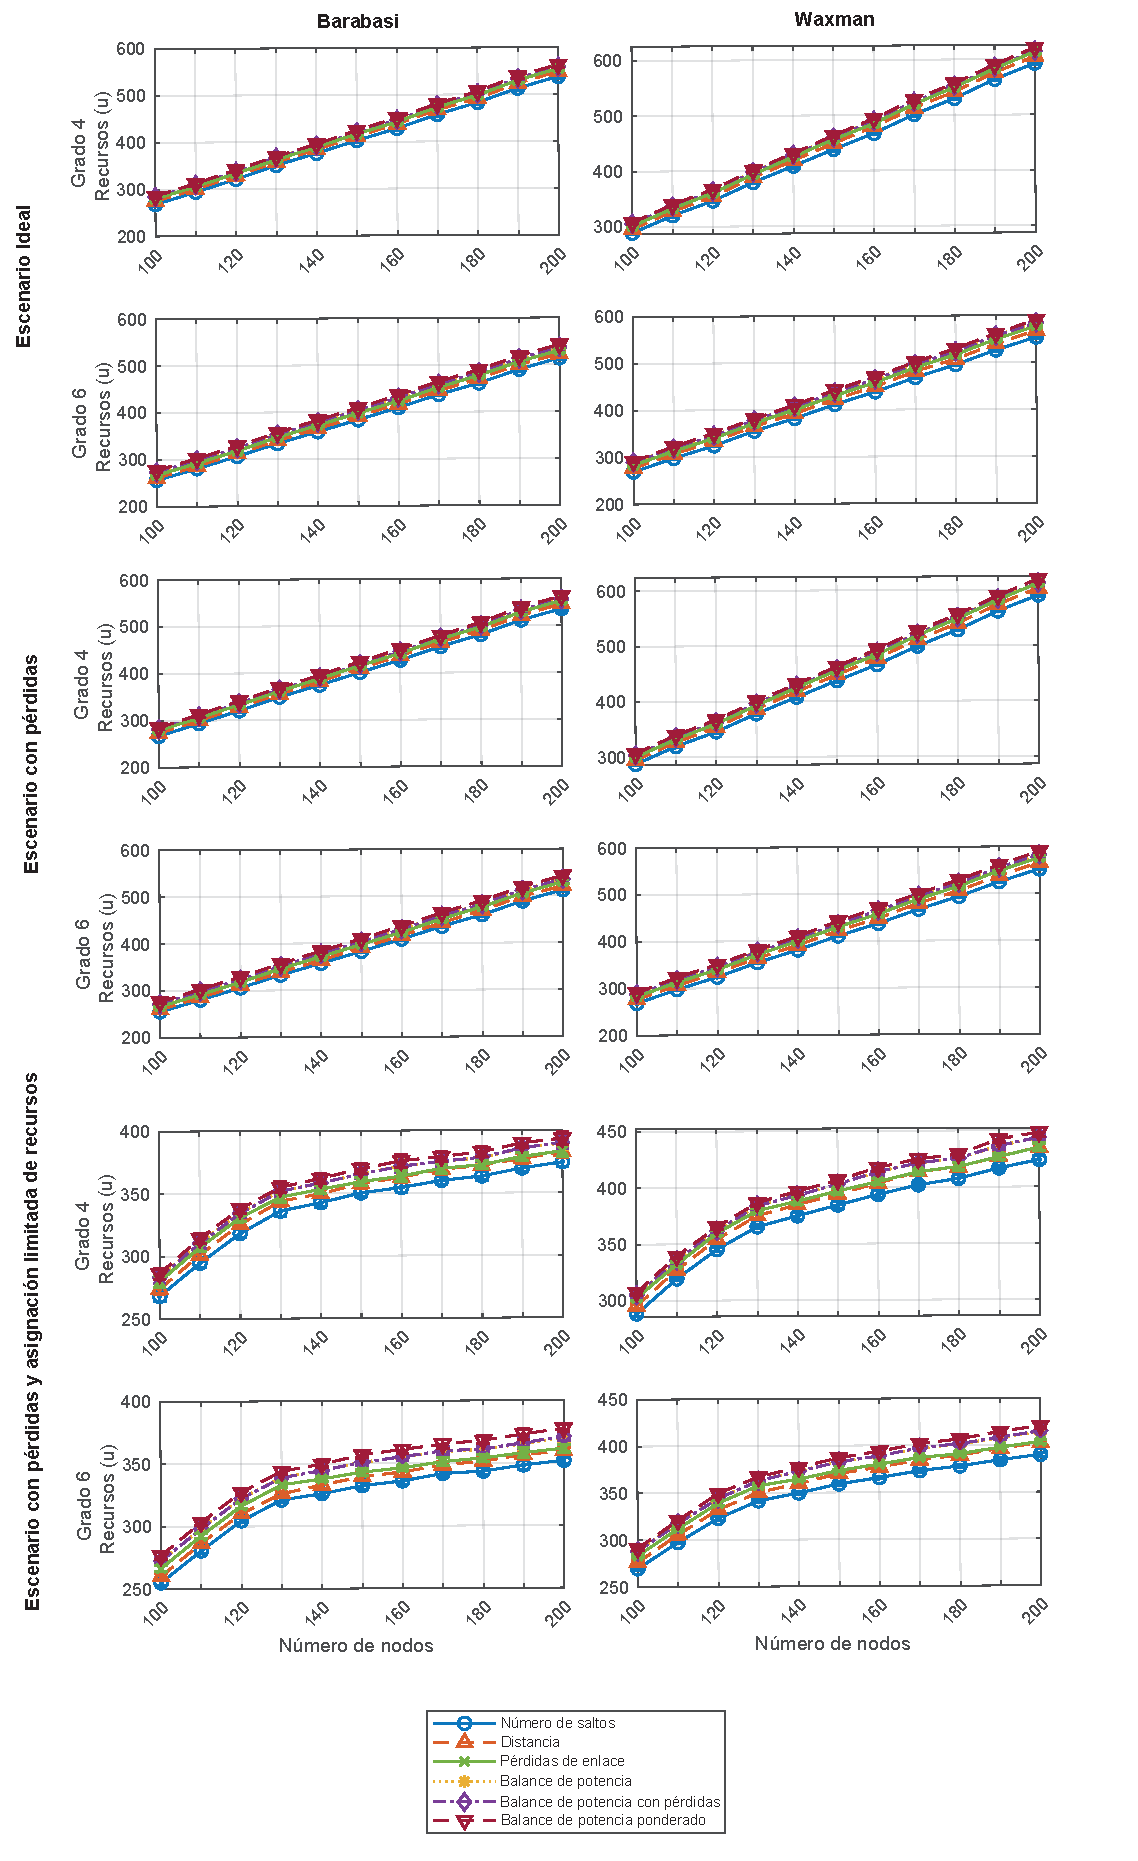
\includegraphics[width=0.85\textwidth,angle=0.9]{fig/05_den2ne/den2ne_17.pdf}
    \caption{Flujo de balance de recursos (\textit{abs\_flux}) - Tres escenarios y dos grados de red.}
    \label{fig:f1}
\end{figure}

La Figura~\ref{fig:f1} ilustra el flujo de balance de recursos para redes con grados de conectividad de 4 a 6, basadas en topologías de Barabási y Waxman, con tamaños comprendidos entre 100 y 200 nodos, y evaluadas con los seis criterios definidos en tres tipos de escenarios: ideal, con pérdidas y con pérdidas bajo limitación de asignación de recursos, respectivamente. Como puede observarse, el flujo crece de manera lineal con el tamaño de la topología, lo que indica que el algoritmo presenta un comportamiento escalable ($\mathcal{O}(n)$), sin estar fuertemente condicionado por el número de nodos involucrados. Únicamente en el último escenario, representado por los cuatro gráficos situados en la parte inferior de la Figura~\ref{fig:f1}, se aprecia un crecimiento de tipo logarítmico, aunque este efecto se debe a la limitación impuesta en la asignación de recursos.\\
\\
Adicionalmente, considerando los seis criterios, parece que el Criterio 1 (número de saltos) ofrece mejores resultados (menor flujo) que el resto, especialmente en topologías Waxman y cuando la conectividad de los nodos aumenta; mientras que el Criterio 6 (balance de potencia ponderado) se presenta como la peor opción, independientemente del escenario (incluso en los casos con pérdidas o con limitaciones de recursos). La discrepancia entre estos criterios puede explicarse por el hecho de que aquellos orientados a minimizar la distancia o el número de saltos hacia el nodo raíz favorecen trayectorias más cortas, mientras que los que consideran la cantidad de recursos a lo largo del camino hacia la raíz tienden a seleccionar trayectorias más largas. Por esta razón, en el Criterio 1 y el Criterio 2 (número de saltos y distancia, respectivamente), el flujo medio de recursos es menor en comparación con el Criterio 3 y el Criterio 6 (balance de potencia y balance de potencia ponderado, respectivamente), donde las trayectorias tienden a ser más largas en promedio, resultando en un mayor flujo de recursos.\\
\\
De la misma forma, la Figura~\ref{fig:f2} ilustra el balance total de recursos para redes con grados de conectividad de 4 a 6, basadas en topologías de Barabási y Waxman, con tamaños comprendidos entre 100 y 200 nodos, y evaluadas con los seis criterios definidos en tres tipos de escenarios: ideal, con pérdidas y con pérdidas bajo limitación de asignación de recursos, respectivamente. Como puede observarse, el balance total de recursos tiende a $0$ en todos los casos, lo cual resulta coherente si se considera que la asignación de recursos sigue la función previamente mostrada en la Figura~\ref{fig:den2ne_16}, cuyo valor medio es $0$. Además, en el escenario ideal todos los criterios producen el mismo resultado, y únicamente en los escenarios con pérdidas se observa cierta variabilidad, debido a que los caminos hacia la raíz (y, por tanto, las pérdidas) difieren. Esto indica que el algoritmo es capaz de compensar todos los recursos en la red, es decir, que todos los nodos tiendan hacia el valor cero (un uso óptimo), poniendo de manifiesto una distribución eficiente, dado que en pocos casos el nodo que actúa como pasarela (root) tendrá que demandar o verter excedentes en niveles superiores de la red.


\begin{figure}[H]
    \centering
    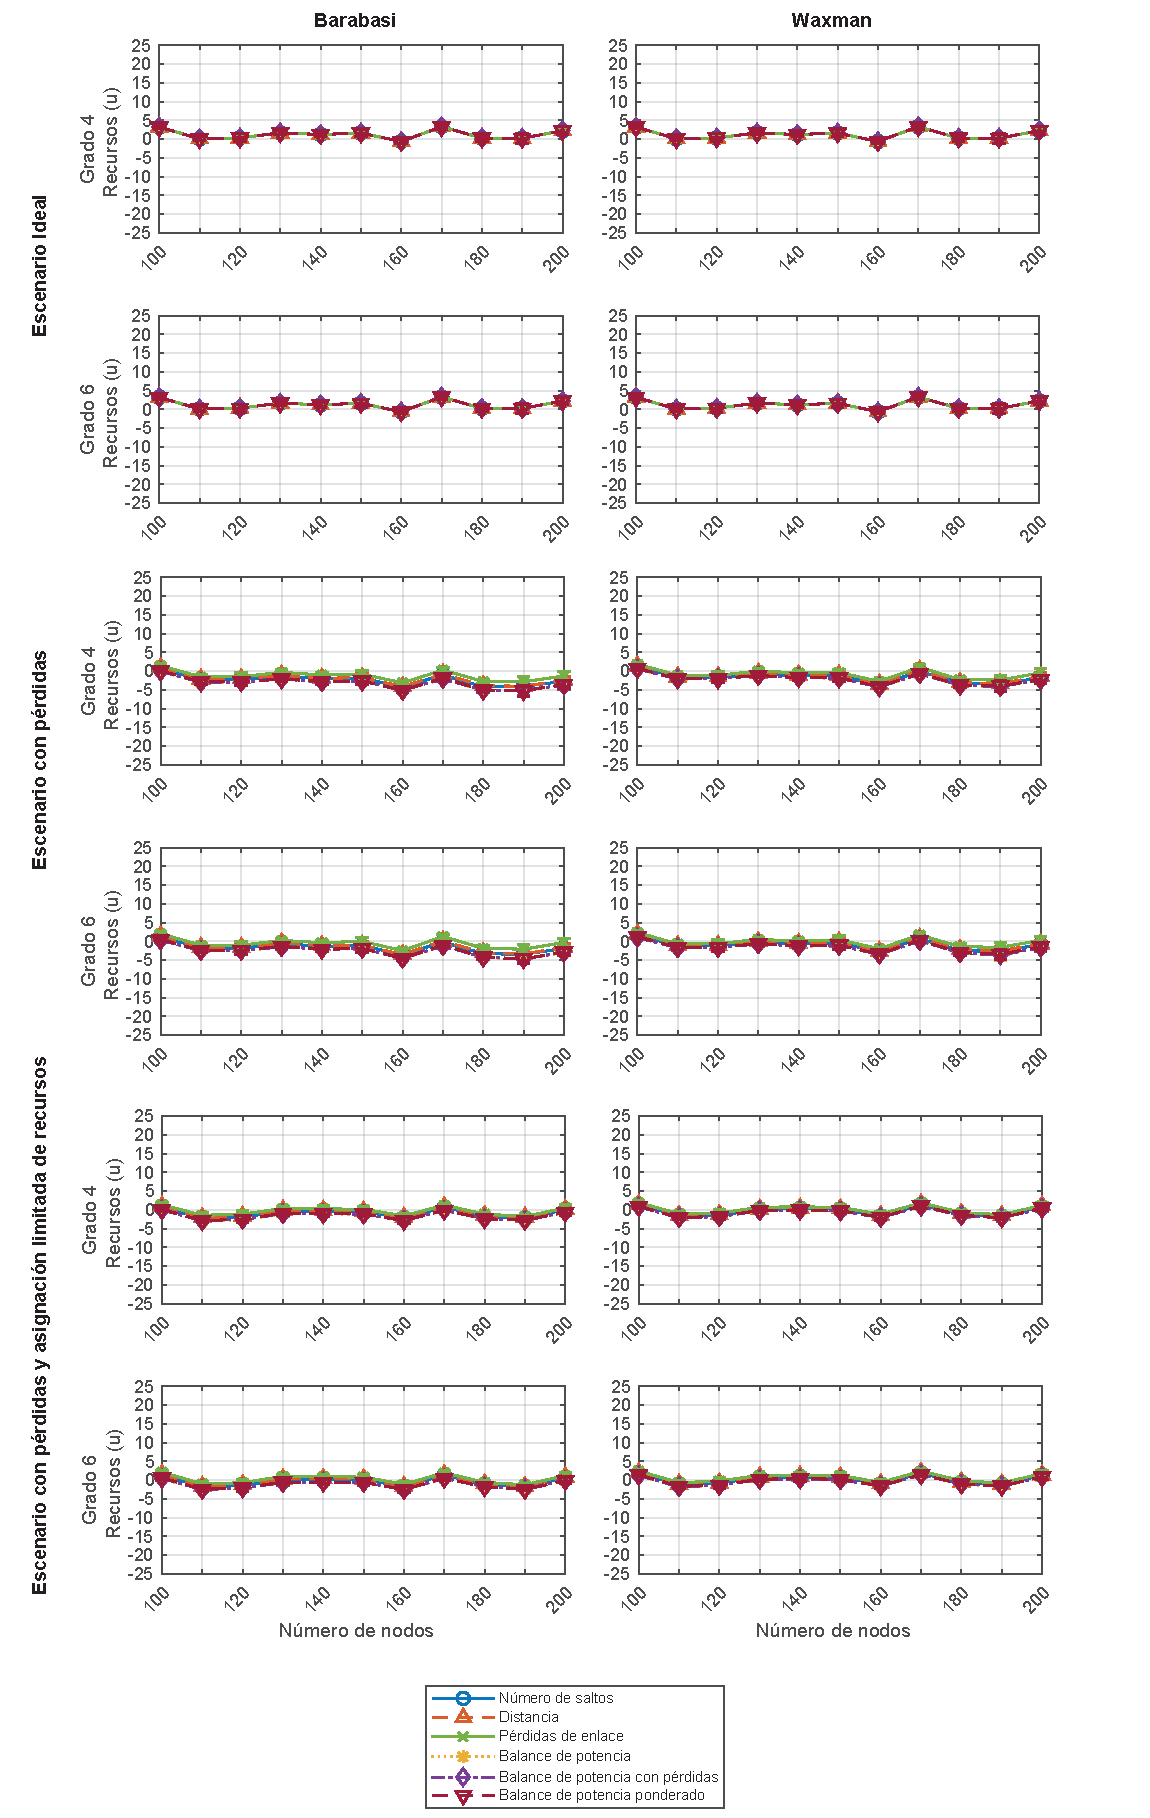
\includegraphics[width=0.85\textwidth,angle=0.9]{fig/05_den2ne/den2ne_18.pdf}
    \caption{Balance total de recursos (\textit{total\_balance}) - Tres escenarios y dos grados de red.}
    \label{fig:f2}
\end{figure}

\subsection{Tiempo de convergencia de la asignación de etiquetas} 

El tiempo de convergencia en la asignación de etiquetas representa el tiempo requerido por el algoritmo para asignar todas las etiquetas jerárquicas desde la raíz hasta el resto de los nodos de la topología. La Figura~\ref{fig:f4} muestra el tiempo de convergencia de la asignación de etiquetas para redes con grados de conectividad de 4 a 6, basadas en topologías de Barabási y Waxman, con tamaños comprendidos entre 100 y 200 nodos, y evaluadas con los seis criterios definidos en tres tipos de escenarios: ideal, con pérdidas y con pérdidas bajo limitación en la asignación de recursos, respectivamente.\\
\\
Como puede observarse, este tiempo de convergencia crece linealmente con el tamaño de la topología, sin verse afectado exponencialmente por el grado de conectividad u otros parámetros. Este hecho refleja una buena escalabilidad potencial del algoritmo, ya que, incluso en los peores casos, el tiempo de convergencia no supera los 15 ms. Además, los seis criterios presentan comportamientos muy similares, sin diferencias significativas. Esto se debe a que el tiempo de convergencia en la asignación de etiquetas depende estrictamente de la primera fase del algoritmo, la cual es independiente del criterio aplicado posteriormente. En caso de existir pequeñas variaciones, estas podrían atribuirse a la naturaleza aleatoria de las pruebas realizadas.


\subsection{Tiempo de convergencia del balance de recursos} 

El tiempo de convergencia en el balanceo de recursos representa el tiempo requerido por el algoritmo para realizar todos los intercambios de recursos hasta que la topología quede balanceada con respecto a la raíz. De igual forma, la Figura~\ref{fig:f3} muestra el tiempo de convergencia del balanceo de recursos para redes con grados de conectividad de 4 a 6, basadas en topologías de Barabási y Waxman, con tamaños comprendidos entre 100 y 200 nodos, y evaluadas con los seis criterios definidos en tres tipos de escenarios: ideal, con pérdidas y con pérdidas bajo limitación en la asignación de recursos, respectivamente. Como puede observarse, y de manera similar al tiempo de convergencia de la asignación de etiquetas, el tiempo de convergencia del balanceo de recursos crece linealmente con el tamaño de la topología, sin verse afectado de forma exponencial por el grado de conectividad u otros parámetros. Este hecho refleja una buena escalabilidad potencial del algoritmo, ya que, incluso en los peores casos, el tiempo de convergencia no supera 1 ms. En consecuencia, el tiempo total de ejecución del algoritmo \gls{d2e} fue inferior a 20 ms en todos los escenarios evaluados.\\
\\
Además, al igual que en la métrica de tiempo anterior, los seis criterios presentan comportamientos muy similares. En este caso, el tiempo de convergencia del balanceo de recursos sí depende de los criterios (a diferencia de la asignación de etiquetas), aunque la propia definición del algoritmo tiene un mayor impacto en este tiempo que el criterio seleccionado. Este aspecto resulta particularmente relevante, ya que los criterios se definen para favorecer una mejor asignación de recursos en distintos escenarios. Por lo tanto, estos resultados demuestran que nuestro algoritmo puede ajustarse y adaptarse a casos de uso específicos sin experimentar variaciones significativas en el tiempo de ejecución. 

\begin{figure}[H]
    \centering
    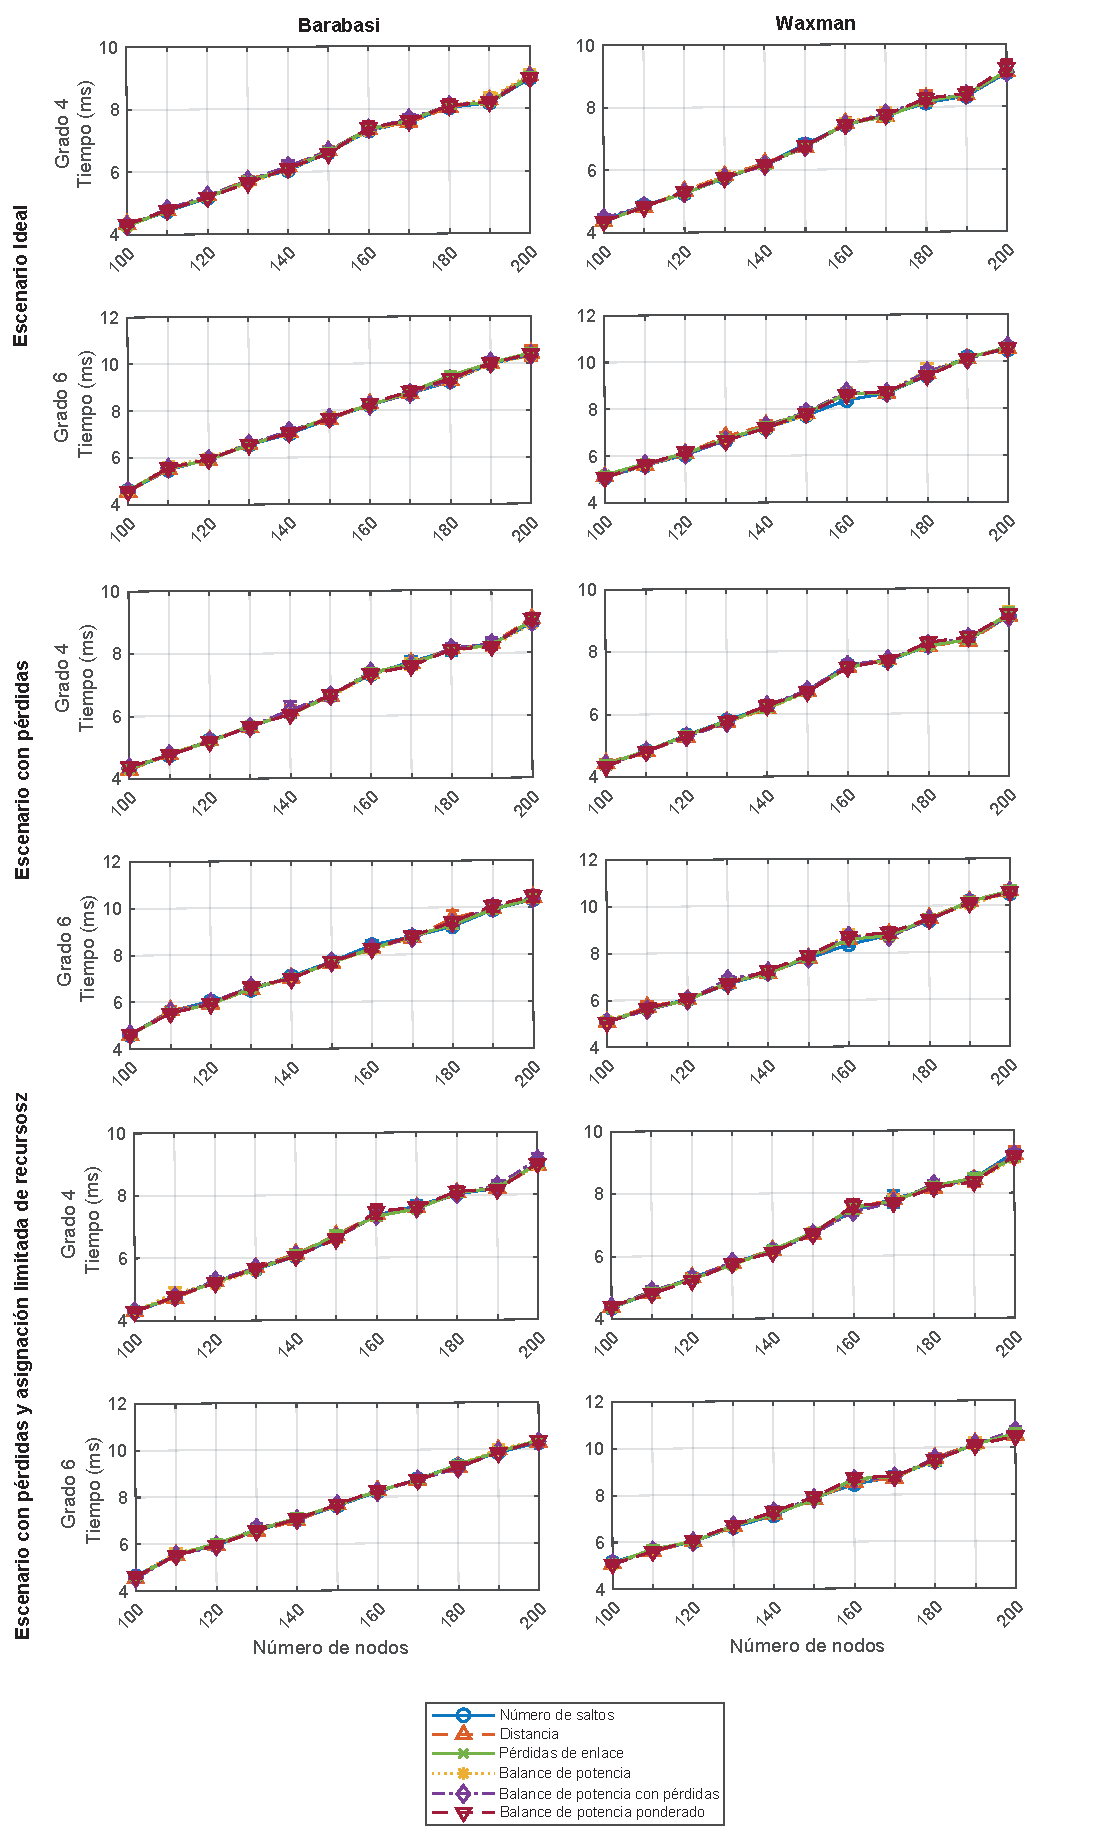
\includegraphics[width=0.85\textwidth]{fig/05_den2ne/den2ne_19.pdf}
    \caption{Tiempo de convergencia de la asignación de etiquetas - Tres escenarios y dos grados de red.}
    \label{fig:f4}
\end{figure}

\begin{figure}[H]
    \centering
    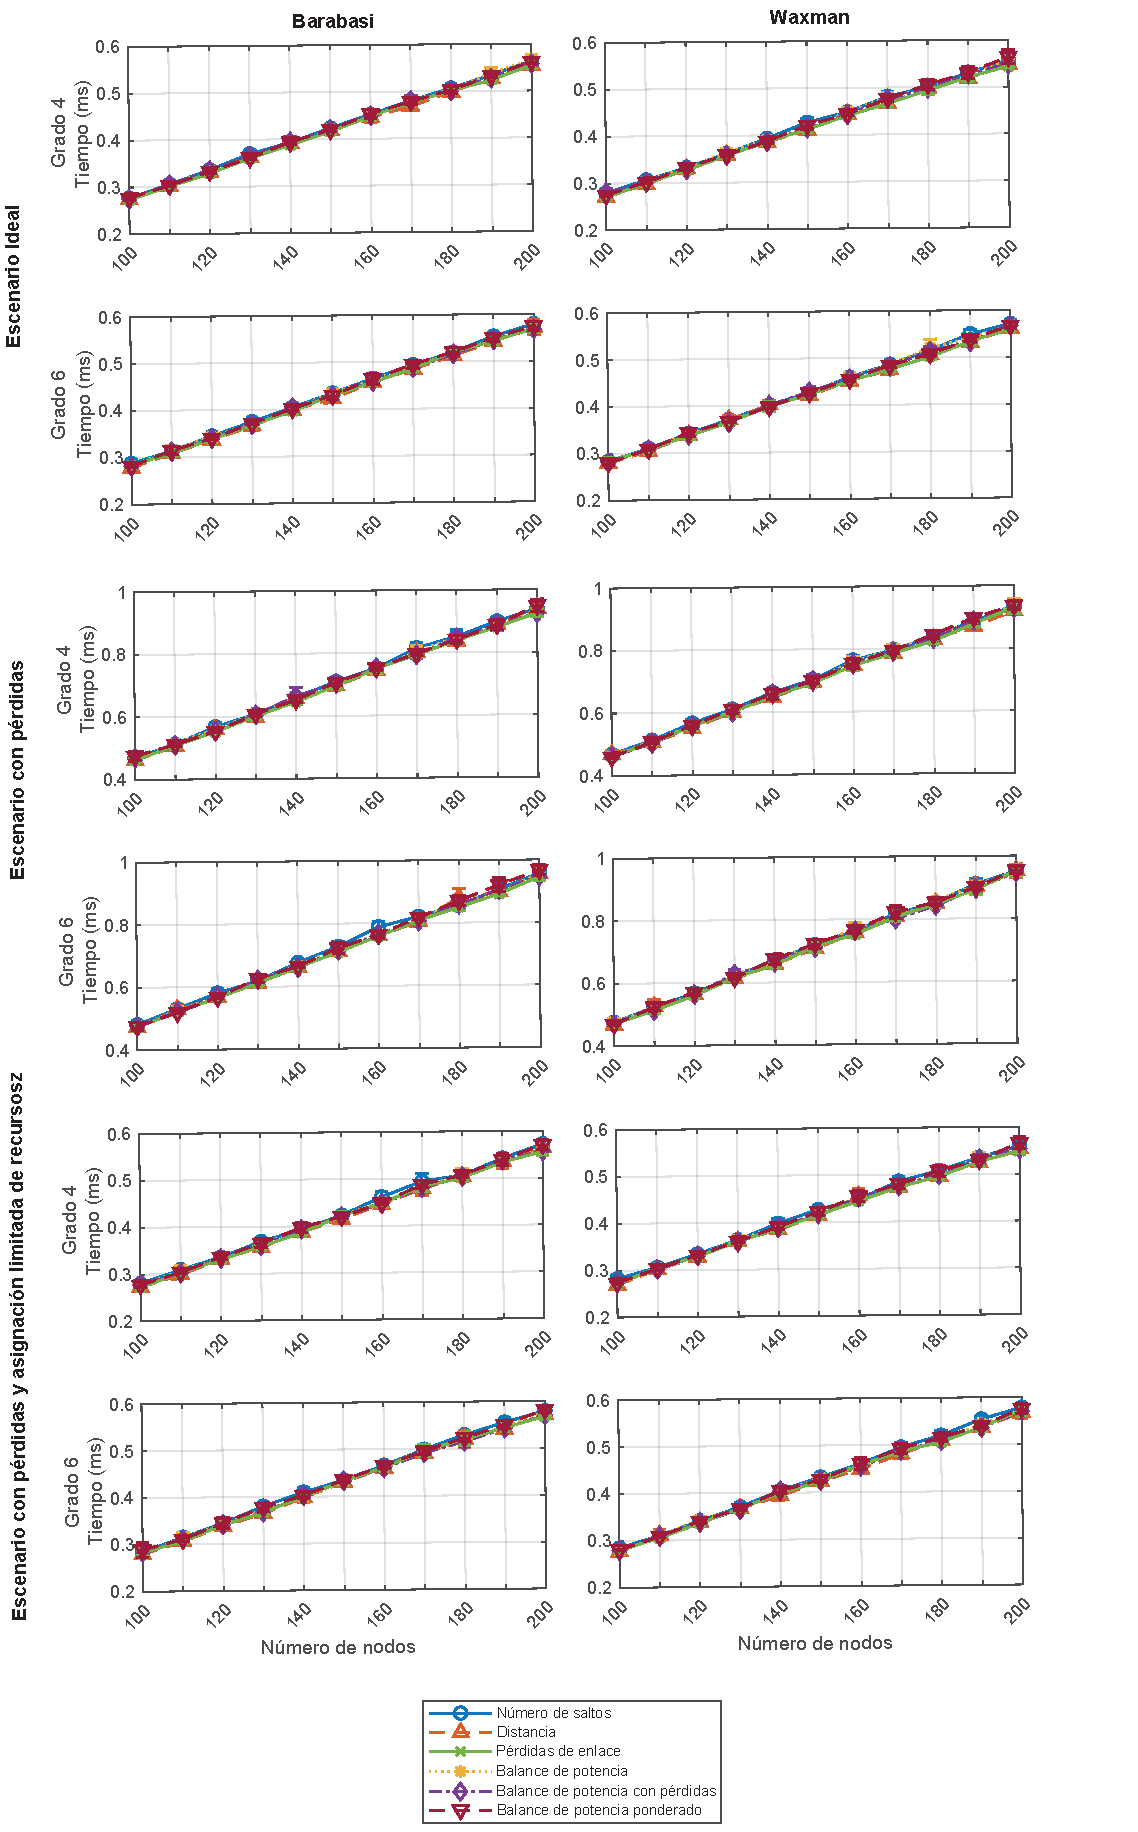
\includegraphics[width=0.85\textwidth]{fig/05_den2ne/den2ne_20.pdf}
    \caption{Tiempo de convergencia del balance de recursos - Tres escenarios y dos grados de red.}
    \label{fig:f3}
\end{figure}

\section{Conclusiones}

En este trabajo se ha presentado \gls{d2e}, un algoritmo para la gestión de recursos en redes densas multi-hop que destaca por su elevada escalabilidad y bajos tiempos de convergencia.\\
\\
El algoritmo descubre los diferentes nodos de la topología y asigna a cada uno de ellos una o varias etiquetas jerárquicas, que representan múltiples rutas hacia el nodo raíz o \textit{gateway}. Posteriormente, redistribuye la carga de trabajo desde los nodos situados en la parte inferior de la jerarquía hasta los niveles superiores. Esta reorganización de recursos puede llevarse a cabo siguiendo distintos criterios: en este trabajo se han evaluado seis como ejemplos representativos, aunque el algoritmo no está limitado a ellos, pudiendo adaptarse fácilmente a otros criterios en función del escenario de aplicación. La evaluación se ha realizado sobre un amplio rango de topologías, con hasta 200 nodos, mostrando tiempos de convergencia reducidos (inferiores a 20 ms) y con un crecimiento lineal. Esta característica resulta especialmente beneficiosa en escenarios con alta movilidad y/o que requieren una mayor fiabilidad. Además, el procedimiento de asignación de etiquetas se ejecuta en solo dos pasos, y cada nodo únicamente necesita almacenar tantas etiquetas como caminos existan hacia el nodo raíz, independientemente del tamaño de la red.\\
\\
Cabe destacar que con \gls{d2e} se sientan las bases para el desarrollo de mecanismos de control, esquemas de encaminamiento basados en etiquetado jerárquico y estrategias de gestión y planificación de recursos en entornos densos y heterogéneos (por ejemplo, \gls{sg}, logística, \textit{edge/fog computing}, entre otros). \gls{d2e} demuestra que es posible combinar asignación jerárquica de rutas, selección de rutas mediante criterios adaptables y una fase de balanceo eficiente con complejidad y requerimientos reducidos, propiedades que resultan críticas en nodos con capacidad limitada. Encajando estas características, directamente con los objetivos de la Tesis.

\chapter{Propuesta de reconfiguración y predicción de errores en redes de distribución eléctrica}
\label{ch:fault_sg}

Partiendo de \gls{d2e} (Capítulo~\ref{ch:den2ne}), que establece las bases para mecanismos de control, esquemas de encaminamiento mediante etiquetado jerárquico y estrategias de gestión/planificación de recursos en entornos densos y heterogéneos, este capítulo explora su aplicación a la optimización y reconfiguración proactiva de redes de distribución eléctrica (\gls{sg}). La combinación de un mecanismo eficiente de descubrimiento/etiquetado con modelos de \gls{ml}/\gls{dl} permite abordar dos retos clave (Analizado en la Sección~\ref{subsubsec:propuestas_optimizacion}): (i) detectar y predecir anomalías o fallos antes de que afecten al servicio, y (ii) coordinar reconfiguraciones automáticas y seguras que minimicen pérdidas y aumenten la resiliencia del sistema.\\
\\
En este capítulo se presenta una propuesta novedosa que integra técnicas de aprendizaje automático (\gls{ml}), y aprendizaje profundo (\gls{dl}) para la predicción temprana de fallos en red con algoritmos de reconfiguración basados en el etiquetado jerárquico propuesto con \gls{d2e}. El sistema propuesto opera en tres capas: (a) adquisición y agregación de telemetría distribuida (sensores, medidores y nodos etiquetados), (b) motores predictivos de \gls{ml}/\gls{dl} que estiman la localización de fallos a corto plazo en la \gls{sg}, y (c) un módulo de decisión que traduce las predicciones en posibles acciones de reconfiguración.\\
\\
Este trabajo nació a raíz de \gls{d2e} (Carrascal \textit{et al.}~\cite{carrascal2024topology}), y se materializó como uno de los primeros TFM que pude dirigir en la universidad (Bartolomé \textit{et al.}~\cite{bartolome2024_smartgrids}), dando lugar a una propuesta (Carrascal \textit{et al.}~\cite{carrascal2024fault}) que pone de manifiesto la versatilidad y capacidad de \gls{d2e} para operar en diferentes dominios y casos de uso finales.

\section{Introducción}

Las \gls{sg} representan la solución futura para las redes de transmisión y distribución eléctrica~\cite{Vu1997,Amin2005}, cuyo objetivo principal es alcanzar una monitorización completa de la red que permita un mejor balance energético entre productores y consumidores. Uno de los aspectos más relevantes de las \gls{sg} es la reconfiguración de la distribución de energía dentro de la propia red. Esto resulta crucial porque permite reencaminar la potencia en caso de fallo en alguno de los enlaces de la red, o simplemente optimizar la distribución según un criterio determinado. Numerosas contribuciones existentes vistas en la Sección~\ref{subsubsec:propuestas_optimizacion} inciden especialmente en este último caso, en el que la reconfiguración mediante optimización reduce pérdidas por propagación o sobrecarga de línea, o actúa sobre otros parámetros eléctricos. De forma general, la mayoría de los algoritmos de reconfiguración aplicados a \gls{sg} que se centran en la resiliencia ante fallos buscan proporcionar rutas de respaldo o caminos alternativos para llevar a cabo la distribución. No obstante, las estrategias propuestas suelen ser siempre reactivas frente al fallo, ya sea de manera centralizada o distribuida.\\
\\
Por ello, en este trabajo nos proponemos generar una estrategia de reconfiguración preventiva, y por tanto proactiva, frente a fallos de red, aprovechando conjuntos de datos reales de \gls{sg} y técnicas de \gls{ml} y \gls{dl}. Como se ha indicado, el enfoque propuesto descansa sobre \gls{d2e}~\cite{carrascal2024topology}. Partimos de dicha base para desarrollar un mecanismo de predicción de fallos que clasifica rutas alternativas obtenidas en la etapa de etiquetado jerárquico suministrado por \gls{d2e}, con el fin de identificar de forma anticipada aquellas con mayor probabilidad de provocar errores en la red. Existen múltiples criterios en las \gls{sg} que pueden dar lugar a fallos en la red, en nuestro caso, analizaremos cuando una línea de la red excede la capacidad física de la misma. En consecuencia, tras el análisis del estado del arte (Sección~\ref{subsubsec:conclu_opt}), las principales aportaciones de nuestro trabajo son las siguientes:

\begin{enumerate}
    \item Una solución de predicción de fallos específicamente orientada a la reconfiguración de \gls{sg}, entrenada y validada con conjuntos de datos reales tal y como se detalla en la Sección~\ref{sec:Faultdatasets}.

    \item Generalizable a topologías de cualquier tipo, forma o tamaño, evaluada con el generador de topologías aleatorias \gls{brite} y parámetros realistas, empleando parámetros inspirados en el modelo \gls{ieee} 123 Node Test Feeder~\cite{Schneider17}. A partir de estas validaciones, hemos estudiado la optimización de varios modelos de \gls{ml} y \gls{dl} para \gls{d2e} mediante selección de características y evaluación del modelo predictivo más adecuado para cada escenario.
\end{enumerate}

Este último punto es de especial interés, dado que, en la literatura revisada, la mayoría de propuestas que emplean \gls{ai}/\gls{ml} suelen tender a generar modelos con un único propósito y un único tipo de red, no siendo extrapolables a otros tipos/casuísticas de \gls{sg}.




\section{Búsqueda y análisis de fuentes de datos}
\label{sec:Faultdatasets}


Para evaluar de manera integral las diferentes técnicas de \gls{ai} aplicadas a la predicción de fallos en escenarios de reconfiguración de \glspl{sg}, resulta esencial disponer de un conjunto de datos de alta calidad. Tanto la calidad como la cantidad de datos son factores determinantes para definir un modelo consistente. En el contexto energético, nuestra experiencia demuestra que existe una menor disponibilidad de conjuntos de datos. La protección de la privacidad de los usuarios en la medición y análisis de su comportamiento energético reduce el número de datasets públicos disponibles, ya que estos dependen principalmente de las compañías eléctricas~\cite{powercons}.\\
\\
No obstante, la búsqueda de la optimización en la distribución de la energía y la reducción del consumo de los usuarios, junto con otras motivaciones medioambientales, ha favorecido la creación de conjuntos de datos públicos en los últimos años. La Tabla~\ref{tab:faultdatasets} muestra varios datasets residenciales analizados, junto con detalles sobre su implementación, tales como la localización, el número de viviendas, el periodo de despliegue, la frecuencia de muestreo y los parámetros eléctricos medidos. Como parte de nuestro análisis, y con el objetivo de evaluar y seleccionar el dataset más adecuado entre los disponibles en la Tabla~\ref{tab:faultdatasets}, se han considerado los siguientes requisitos:


\begin{itemize}
    \item \textbf{Cantidad}: Es fundamental revisar la cantidad de datos disponibles en cada dataset, asegurando que incluyan mediciones de un número amplio de viviendas y que abarquen periodos prolongados de tiempo para analizar de manera efectiva los patrones de consumo energético.

    \item \textbf{Calidad}: La calidad de los datos depende de la resolución de las mediciones. Datasets como \textit{REDD} y \textit{BLUED} ofrecen frecuencias de muestreo elevadas, lo que permite una mejor desagregación del consumo energético y un análisis más representativo de los patrones energéticos.
    
    \item \textbf{Localización}: La localización de los datos es relevante, ya que influye en las diferencias de voltaje entre países. Por ejemplo, datasets de Estados Unidos, como \textit{BLUED}, operan a menos de 120V, mientras que conjuntos europeos como \textit{ECO} trabajan hasta 230V.
    
    \item \textbf{Parametrización}: Las muestras incluyen tensión (V), corriente (I) y potencia (tanto la activa (P), la reactiva (Q), y la aparente (S)), cada una asociada a una marca temporal y un identificador correspondiente a la vivienda. Algunos datasets, como \textit{HUE} y \textit{SustDataED}, también incorporan datos ambientales, lo cual resulta relevante para comprender el impacto de las condiciones climáticas con la generación de potencia renovable.
    
    \item \textbf{Generación Fotovoltaica}: En el contexto de las \glspl{sg}, es esencial elegir conjuntos de datos que incluyan información sobre generación de energía renovable, como \textit{Smart*} y \textit{SustDataED}.
\end{itemize}

Entre los datasets analizados, se seleccionó especialmente \textit{SustDataED}, debido al elevado número de usuarios con perfiles tanto de consumo, como de producción a lo largo de un periodo extenso de tiempo. Asimismo, resulta clave que las muestras presenten una buena resolución y que ofrezcan información en tiempo real sobre las condiciones climáticas de la ubicación en la que se encuentran las viviendas. En las siguientes secciones, se examina en detalle este conjunto de datos y se describen los principales criterios de diseño aplicados para generar el dataset final, elaborado a partir de \textit{SustDataED} y complementado con la herramienta PVWatts, que finalmente se utilizó en nuestra evaluación.

\begin{sidewaystable}
    \centering
     % o \scriptsize si quieres reducir aún más la fuente
    \begin{tabularx}{\textheight}{|l|X|c|c|c|c|}
        \hline
        \textbf{Nombre} & \textbf{Localización} & \textbf{Residencias} & \textbf{Periodo (días)} & \textbf{Resolución} & \textbf{Parámetros} \\ \hline
        \textit{AMPds2} \cite{ampds2} & Vancouver (Canadá) & 1 & 730 & 60s & I, V, P, S, F, pf \\ \hline
        \textit{BLUED} \cite{blued} & Pittsburgh (EE.\,UU.) & 1 & 8 & 83.33$\mu$s & I, V, eventos switch \\ \hline
        \textit{ECO} \cite{eco} & Suiza & 6 & 244 & 1s & P \\ \hline
        \textit{GREEND} \cite{greend} & Italia y Austria & 9 & 310 & 1s & P \\ \hline
        \textit{HUE} \cite{hue} & Columbia Británica (Canadá) & 28 & 60 & 1s & P \\ \hline
        \textit{iAWE} \cite{iawe} & Nueva Delhi (India) & 1 & 73 & 1s & V, I, P, S \\ \hline
        \textit{REDD} \cite{redd} & Boston (EE.\,UU.) & 6 & 119 & 66.66$\mu$s & I, V, P \\ \hline
        \textit{Smart*} \cite{smart*} & Massachusetts (EE.\,UU.) & 3 & 90 & 60s & P, S, V, I \\ \hline
        \textit{SustDataED} \cite{sustdata} & Madeira (Portugal) & 50 & 1144 & 60s & I, V, P, Q, S \\ \hline
        \textit{UK-DALE} \cite{ukdale} & Reino Unido & 5 & 499 & 62.5$\mu$s & P, estados de switch \\ \hline
    \end{tabularx}
    \caption{Comparación de datasets sobre el consumo público de energía eléctrica.}
    \label{tab:faultdatasets}
\end{sidewaystable}

\subsection{Análisis del dataset - SustDataED}

El dataset \textit{SustDataED}~\cite{sustdata} fue creado como parte del proyecto de investigación SINAIS, cuyo objetivo es proporcionar retroalimentación ecológica a los usuarios para fomentar un comportamiento energético sostenible y un mayor uso de fuentes de energía renovable. Este dataset abarca cinco años de datos de consumo y producción energética de 50 hogares en la ciudad de Funchal (Madeira, Portugal), divididos en tres despliegues diferentes. Esto implica que no existen mediciones de los 50 hogares de forma simultánea a lo largo de los cinco años del proyecto, sino agrupadas en tres conjuntos separados. La Figura~\ref{fig:demographics} muestra los tres despliegues mencionados. Dado que trabajamos con mediciones de consumo y generación que están parcialmente correlacionadas con condiciones meteorológicas y temporales, seleccionaremos el periodo de tiempo con el mayor número de hogares desplegados simultáneamente. En nuestro caso, se elige el primer despliegue, en el cual se dispone de mediciones de hasta 23 hogares de manera simultánea.
 

\begin{figure}[ht!]
    \centering
    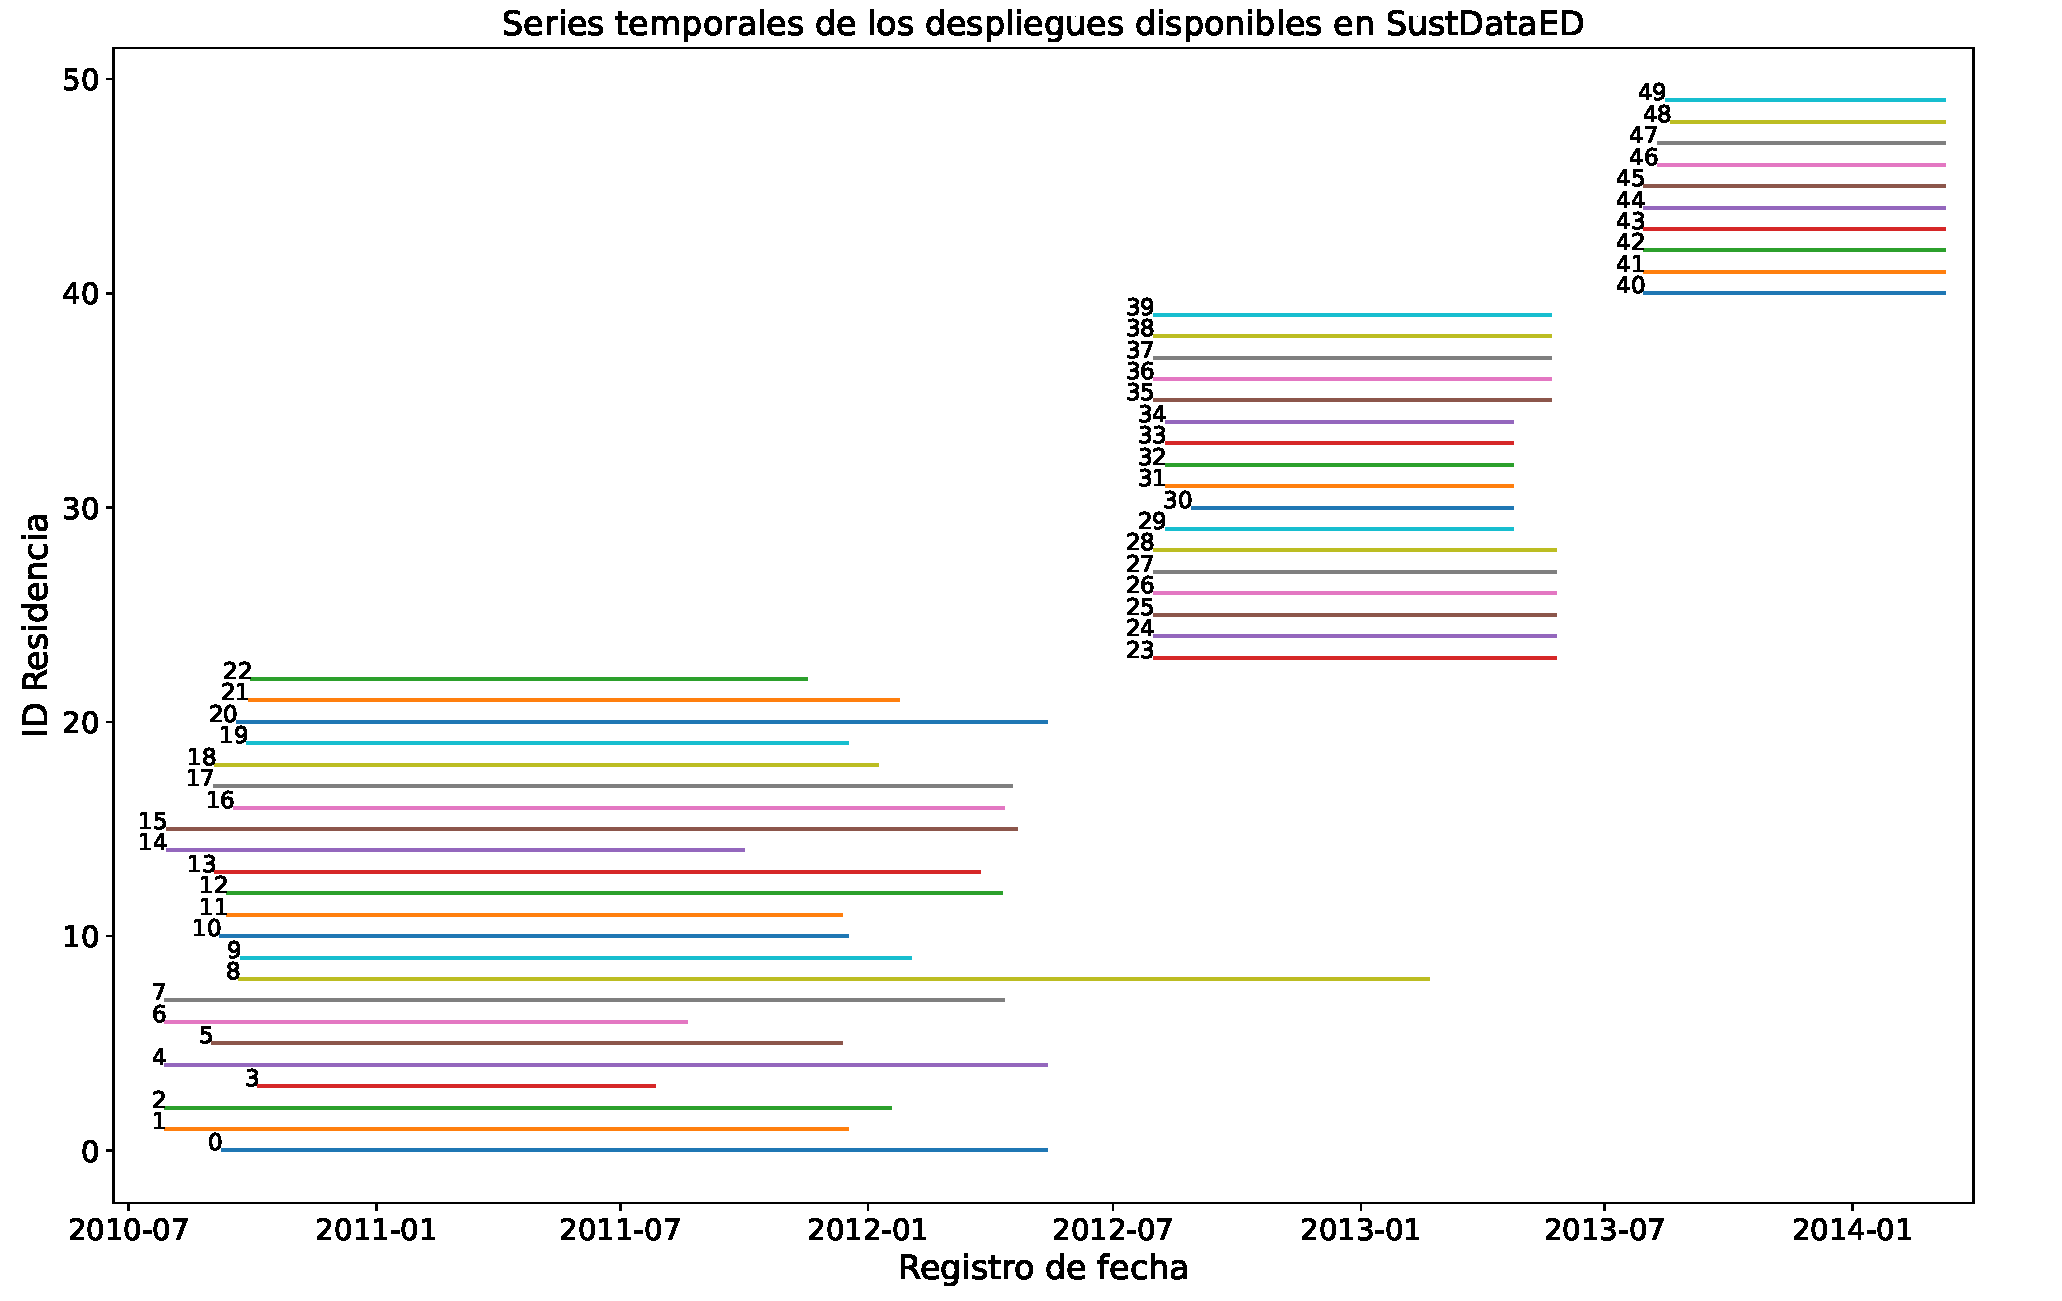
\includegraphics[width=\textwidth]{fig/06_fault_sg/fault_sg_01.pdf}
    \caption{Series temporales de los diferentes despliegues del dataset \textit{SustDataED}.}
    \label{fig:demographics}
\end{figure}

Los datos disponibles en \textit{SustDataED} son bastante variados. La Tabla~\ref{tab:SustDataEDMeasurements} muestra los diferentes tipos de mediciones incluidos en el dataset. Sin embargo, no todas ellas son relevantes para este estudio. Por ejemplo, un alto nivel de granularidad, como las mediciones de eventos de potencia o de eventos de usuario, no es necesario para nuestro análisis. Como se observa en la Tabla~\ref{tab:SustDataEDMeasurements}, las mediciones relacionadas con la producción de energía presentan cierta incertidumbre. A primera vista, \textit{SustDataED} resulta adecuado porque ofrece mediciones reales de producción fotovoltaica. No obstante, estos datos se reportan como valores agregados y corresponden a un sistema fotovoltaico que abastece a todos los hogares del despliegue, sin especificar información sobre las dimensiones del sistema. Además, no está claro si el tamaño del sistema fotovoltaico aumenta con el tiempo, lo que dificulta el análisis a nivel individual de cada hogar.


\begin{table}[ht!]
\centering
%\resizebox{0.6\textwidth}{!}{%
\begin{tabular}{|l|c|}
\hline
\textbf{Tipo de medida}                       & \textbf{Utilidad} \\ \hline
Mediciones del consumo energético                    & \checkmark             \\ \hline
Mediciones de la producción de energía                    & \textbf{?}             \\ \hline
Mediciones demográficas                           & \checkmark              \\ \hline
Mediciones de las condiciones ambientales y climáticas & \checkmark              \\ \hline
Mediciones de eventos de usuario                           & \text{\sffamily X}             \\ \hline
Mediciones de eventos de potencia                         & \text{\sffamily X}               \\ \hline
\end{tabular}%
%}
\caption{Tipos de mediciones en el dataset \textit{SustDataED}.}
\label{tab:SustDataEDMeasurements}
\end{table}


\subsection{Deficiencias del dataset - SustDataED}

Dado que la literatura sobre \textit{SustDataED} no ofrecía claridad en cuanto a las mediciones de producción de energía fotovoltaica a nivel individual de cada hogar, se buscó una alternativa para conformar un nuevo conjunto de datos de producción. Por ello, se propuso llevar a cabo simulaciones de producción fotovoltaica en la ciudad de Funchal, con las características y dimensiones de un sistema fotovoltaico convencional, para así tener una estimación coherente de la generación a nivel de un hogar. Para realizar esta simulación de datos de producción, se eligieron dos herramientas con el fin de comparar y garantizar que los resultados obtenidos fueran consistentes:


\begin{itemize}
    \item \textbf{Global Solar Atlas}~\cite{globalsolar}: Esta plataforma está financiada por el Programa de Asistencia para la Gestión del Sector Energético (ESMAP), con el objetivo de mapear los recursos de energía renovable a nivel mundial, proporcionando acceso tanto a datos promediados a largo plazo como a datos en tiempo real para cualquier ubicación del planeta.

    \item \textbf{PVWatts}~\cite{pvwatts}: Esta plataforma es proporcionada por el Laboratorio Nacional de Energías Renovables (NREL), que forma parte del Departamento de Energía de los Estados Unidos.

\end{itemize}

Para cada herramienta, la ubicación se fijó en Funchal (Portugal), dado que el análisis debe corresponder a los datos recogidos en el conjunto \textit{SustDataED}. Una vez establecida la localización, se configuró el sistema fotovoltaico para cada hogar y se extrajeron las capas de datos relevantes, como el \gls{dni} ($\frac{kWh}{m^{2}}$) y el \gls{pvout} ($\frac{kWh}{kWp}$), que son parámetros clave para estimar la producción de los sistemas fotovoltaicos. \\
\\
Además, los factores climáticos desempeñan un papel crucial en la verificación de la consistencia de la energía generada. Según las clasificaciones climáticas de Köppen y Trewartha, Funchal presenta un clima mediterráneo con influencias oceánicas, o bien un clima templado con veranos secos. Al estar situada en una zona subtropical, la ciudad experimenta variaciones diarias mínimas de temperatura, lo que se traduce en condiciones relativamente estables a lo largo del año.\\
\\
Tras configurar ambos sistemas, se alinearon las fechas correspondientes a las series temporales de \textit{SustDataED} para recopilar los datos de producción fotovoltaica. En ambas herramientas, tal como se muestra en la Figura~\ref{fig:DNIpvoutVS}, se llevó a cabo un análisis comparativo de los mismos parámetros, \gls{dni} y \gls{pvout}, durante los mismos periodos de tiempo. Los resultados, ilustrados en la Figura~\ref{fig:DNIpvoutVS}, resultaron ser prácticamente idénticos. Una vez verificada esta consistencia entre las dos herramientas para la simulación de valores de producción fotovoltaica, se seleccionó \textit{PVWatts} debido a su capacidad de exportar datos de forma más sencilla, lo que facilitó la integración con los datos de \textit{SustDataED} para la construcción del dataset final.

\begin{figure}[ht!]
    \centering
    \begin{minipage}{0.47\textwidth}
        \centering
        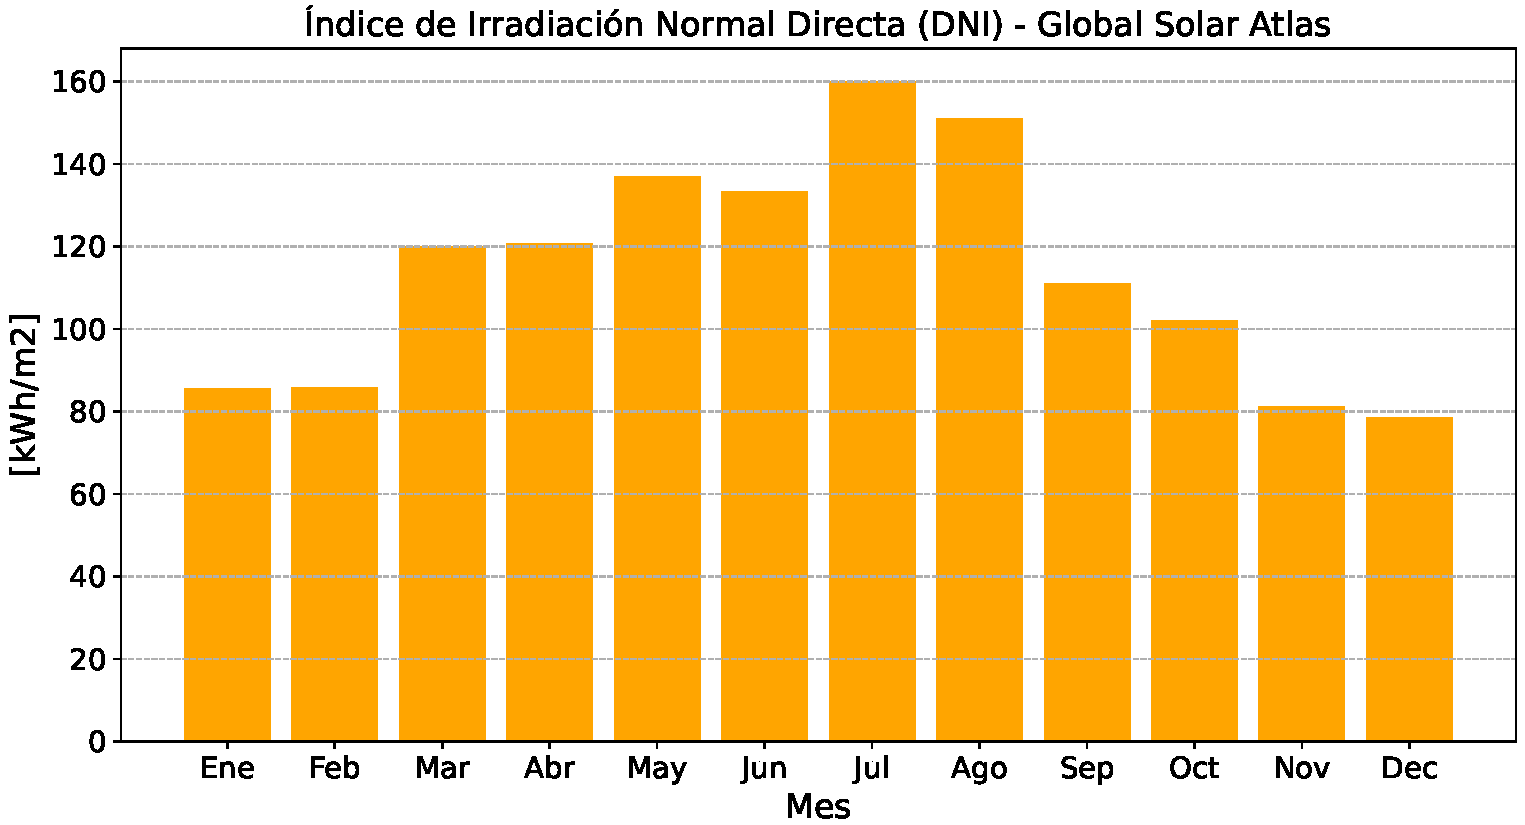
\includegraphics[width=\linewidth]{fig/06_fault_sg/fault_sg_02a.pdf}
        \subcaption{\textit{Global Solar Atlas} - DNI}
    \end{minipage}
    \hfill
    \begin{minipage}{0.47\textwidth}
        \centering
        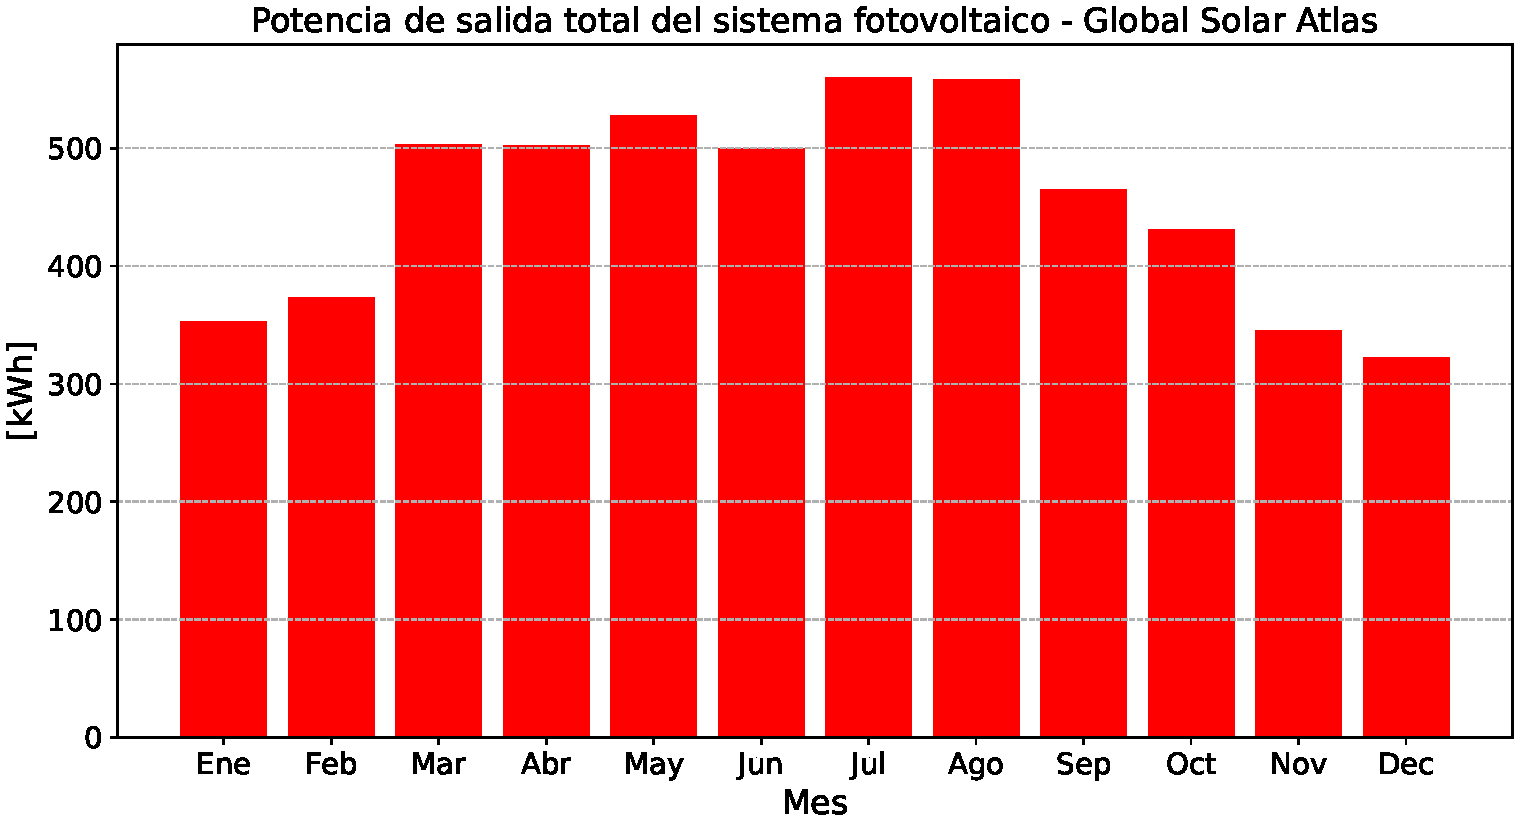
\includegraphics[width=\linewidth]{fig/06_fault_sg/fault_sg_02b.pdf}
        \subcaption{\textit{Global Solar Atlas} - PVOUT}
    \end{minipage}
    
    \vspace{0.5cm} % Espacio entre filas
    
    \begin{minipage}{0.47\textwidth}
        \centering
        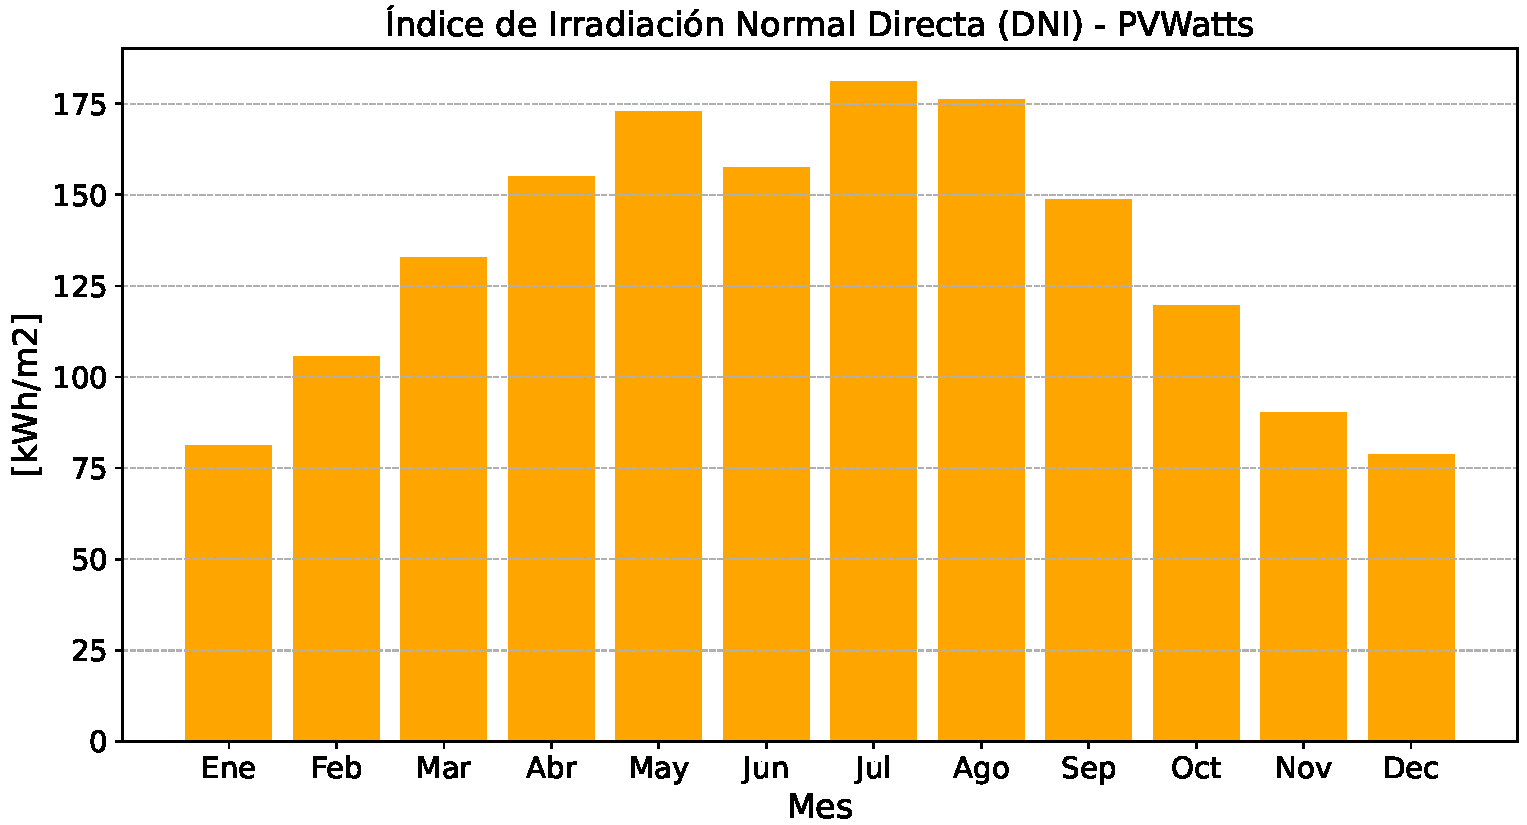
\includegraphics[width=\linewidth]{fig/06_fault_sg/fault_sg_02c.pdf}
        \subcaption{\textit{PVWatts} - DNI}
    \end{minipage}
    \hfill
    \begin{minipage}{0.47\textwidth}
        \centering
        \includegraphics[width=\linewidth]{fig/06_fault_sg/fault_sg_02d.pdf}
        \subcaption{\textit{PVWatts} - PVOUT}
    \end{minipage}
    
    \caption{Comparación entre \textit{Global Solar Atlas} y \textit{PVWatts}, valores mensuales totales de producción de energía fotovoltaica (PVOUT) frente a la irradiación directa normal (DNI).}
    \label{fig:DNIpvoutVS}
\end{figure}

Además, se realizó un análisis de correlación exhaustivo sobre los parámetros de generación de energía fotovoltaica tanto del conjunto de datos \textit{SustDataED} como de \textit{PVWatts}, con el objetivo de evaluar de forma concluyente la fiabilidad de los datos de producción energética. Al examinar la correlación entre las variables climáticas y la generación de energía en ambos conjuntos de datos, tal como se muestra en la Figura~\ref{fig:corrSUST_PVWATTS}, emergen patrones diferenciados.\\
\\
Para \textit{SustDataED} (Figura~\ref{fig:corrSUST_PVWATTS} (a)), es evidente que la temperatura presenta una correlación débil con la potencia generada, arrojando un coeficiente de tan solo 0.279. Esta falta de correlación significativa se repite en otras variables, lo que dificulta el análisis de la producción de energía en relación con las condiciones climáticas. En contraste, para el conjunto de datos \textit{PVWatts} (Figura~\ref{fig:corrSUST_PVWATTS} (b)), la mayoría de los parámetros muestran un alto grado de correlación, cercano a la unidad. Por ejemplo, la correlación entre la irradiancia del plano del array, que es la cantidad total de radiación solar que incide sobre la superficie de un panel solar, y la generación de potencia es prácticamente ideal, con un coeficiente de 0.999, como se observa claramente en la gráfica.


\begin{figure}[ht!]
    \centering
    \begin{minipage}{0.39\textwidth}
        \centering
        \includegraphics[width=\linewidth]{fig/06_fault_sg/fault_sg_03a.pdf}
        \subcaption{Parámetros fotovoltaicos - \textit{SustDataED}}
    \end{minipage}
    \hfill
    \begin{minipage}{0.54\textwidth}
        \centering
        \includegraphics[width=\linewidth]{fig/06_fault_sg/fault_sg_03b.png}
        \subcaption{Parámetros fotovoltaicos - \textit{PVWatts}}
    \end{minipage}

    \caption{Comparación mediante matrices de correlación de los parámetros de producción fotovoltaica.}
    \label{fig:corrSUST_PVWATTS}
\end{figure}

\begin{figure}[ht!]
    \centering
    \includegraphics[width=\linewidth]{fig/06_fault_sg/fault_sg_04.pdf}
    \caption{Patrones de correlación entre los parámetros de producción en \textit{PVWatts}.}
    \label{fig:corrUST_PVWATTS_graphs}
\end{figure}

Como se ilustra en la Figura~\ref{fig:corrUST_PVWATTS_graphs}, el diagrama de dispersión correspondiente a la correlación de los parámetros de producción de \textit{PVWatts}, revela que los parámetros más significativos para la generación de energía fotovoltaica son: la irradiancia del plano del array del panel solar y la temperatura de las celdas solares. Dadas las limitaciones de los datos de producción de \textit{SustDataED}, especialmente en términos de precisión y granularidad, se decidió utilizar los datos de producción simulados mediante la herramienta \textit{PVWatts}. Esta elección se sustenta en la consistencia mostrada por los datos de \textit{PVWatts} al compararlos con los resultados del \textit{Global Solar Atlas}, y la capacidad que tiene la herramienta para exportar datos de simulación para la integración de los datos de generación fotovoltaica en el dataset final. En la siguiente sección, se presentará el dataset final, sus características clave, y la organización de los ficheros resultantes. 

\subsection{Dataset final}
\label{subsec:keymondata}
Tras identificar y abordar las limitaciones de \textit{SustDataED} mediante la incorporación de la herramienta \textit{PVWatts} para los datos de generación fotovoltaica, se procesó el conjunto completo de datos con el fin de crear el dataset final. El flujo de procesamiento de datos se muestra en la Figura~\ref{fig:dataprocessing}. Como se observa, existen dos ramas principales: la primera procede del conjunto \textit{SustDataED} e incluye todos los datos de consumo de los hogares, mientras que la segunda corresponde a los datos de generación fotovoltaica. De los 50 hogares, solo se seleccionaron 23 pertenecientes al primer despliegue, como se indicó previamente. Posteriormente, se generaron 23 perfiles de generación fotovoltaica, conformando finalmente 23 archivos de cargas netas reales, que representan la suma de consumo y generación. Los campos finales incluidos en el dataset final se detallan en la Tabla~\ref{tab:datacombinacion}.

\begin{table}[H]
  \centering
  \resizebox{\textwidth}{!}{  
  \begin{tabular}{|c|c|c|}
  \hline
  \multicolumn{1}{|c|}{\textbf{Campo}} & \multicolumn{1}{c|}{\textbf{Descripción}} & \textbf{Unidades} \\ \hline
  \textit{timestamp} & Instante temporal de medida & datetime \\ \hline
  \textit{datetime} & Fecha del valor promedio & datetime \\ \hline
  \textit{H} & Hora del valor promedio & - \\ \hline
  \textit{iid} & Identificador de vivienda & - \\ \hline
  \textit{Diffuse Irradiance} & Índice de radiación difusa (DIF) & W/m2 \\ \hline
  \textit{Plane of Array Irradiance} & Índice de radiación en el plano del array (POA) & W/m2 \\ \hline 
  \textit{Ambient Temperature} & Temperatura ambiente & C \\ \hline
  \textit{Cell Temperature} & Temperatura de las células solares & C \\ \hline
  \textit{DC Array Output} & Potencia de salida DC del array & W \\ \hline
  \textit{AC System Output} & Potencia de salida AC del sistema & W \\ \hline
  \textit{Pavg} & Potencia consumida & W \\ \hline
  \textit{Dif} & Carga neta calculada & W \\ \hline
  \end{tabular}
  }
  \caption{Características principales del dataset final (\textit{KeyMonData}).}
  \label{tab:datacombinacion}
\end{table}

\begin{sidewaysfigure}
    \centering
    \includegraphics[width=\textwidth]{fig/06_fault_sg/fault_sg_05.drawio.pdf}
    \caption{Esquema de procesamiento de datos para la generación del dataset final.}
    \label{fig:dataprocessing}
\end{sidewaysfigure}

Este nuevo conjunto de datos requirió un procesamiento adicional para limitar tanto su tamaño como la serie temporal, de modo que se ajustara al despliegue especificado. Además, para hacerlo más manejable, los datos fueron sintetizados. Concretamente, \textit{SustDataED} ofrece medidas con una resolución a nivel de minuto; sin embargo, trabajar con muestras minuto a minuto resulta innecesario, dado que las variaciones de consumo son mínimas. Por ello, se redujo la resolución a muestras horarias. Así, si el primer despliegue se restringe a un año de duración, se obtienen 8760 intervalos temporales ($24\: h \times 365\: dias$) por cada hogar, para un total de 23 hogares.\\
\\
En cuanto a la convención de nombres de archivos, cada fichero fue etiquetado como \textit{load\_x.csv}, donde $x$ corresponde al identificador del hogar para las cargas calculadas. En consecuencia, se generaron un total de 23 archivos de cargas (\textit{load\_x.csv}), cada uno con 8760 intervalos temporales. Tras el procesamiento, limpieza y síntesis, el nuevo dataset fue denominado \textit{KeyMonData} y se ha puesto a disposición pública para su uso por parte de cualquier interesado~\cite{paulaTFM}.



\section{Algoritmo de reconfiguración y propuesta de extensión}  

El algoritmo de reconfiguración para las \gls{sg}, sobre el cual se construirán los modelos de \gls{ml} y \gls{dl}, es \gls{d2e}~\cite{carrascal2024topology}. Como se ha explicado anteriormente, ver Capítulo~\ref{ch:den2ne}, \gls{d2e} es un algoritmo diseñado para el descubrimiento de rutas en redes densas y heterogéneas, permitiendo automatizar el proceso de encaminamiento desde los nodos hoja hasta el nodo raíz de la topología, al tiempo que gestiona de forma eficiente el uso compartido de recursos. En el contexto específico de una \gls{sg}, el nodo raíz se define como aquel que dispone de conexión directa con la red de distribución eléctrica, mientras que los nodos ``hoja'' representan el resto de nodos de la \gls{sg}. \\
\\
Para explicar con mayor detalle el proceso de reconfiguración seguido por \gls{d2e}, la Figura~\ref{fig:load_power_balancing} ilustra un escenario de redistribución de carga dentro de una \gls{sg}, similar al ejemplo de la topología \gls{ieee} 5-bus. En verde se muestran los nodos con superávit de carga, que puede ser ofrecida a otros nodos de la red. En naranja se destacan los nodos que demandan energía de sus vecinos o, en última instancia, del nodo raíz. Sin embargo, calcular todas las posibles soluciones de redistribución de carga puede ser computacionalmente complejo en un tiempo razonable. Por ejemplo, la Figura~\ref{fig:load_power_balancing} (a) muestra una redistribución subóptima de recursos, que ocurre cuando los vecinos toman decisiones locales, lo que lleva a que la mayoría de solicitudes se dirijan al nodo con un superávit de +100 (insuficiente para cubrir toda la demanda). En cambio, la Figura~\ref{fig:load_power_balancing} (b) representa un escenario de distribución óptima, que requiere un enfoque más sofisticado para la distribución eficiente de recursos.


\begin{figure}[H]
    \centering
    \includegraphics[width=0.9\linewidth]{fig/06_fault_sg/fault_sg_06.pdf}
    \caption{Ejemplo de redistribución de carga en una SG.}
    \label{fig:load_power_balancing}
\end{figure}

Para abordar este problema en las \gls{sg}, \gls{d2e} propone una solución en tres fases. La primera fase, mostrada en la Figura~\ref{fig:labelspropagation}, consiste en explorar todas las rutas posibles desde el nodo raíz hasta cada nodo de la topología (mecanismo similar al visto en la Sección~\ref{subsec:fase1}). Esta exploración, como se ilustra en la figura, se realiza mediante el uso de etiquetas. El proceso comienza en el nodo raíz, que genera la primera etiqueta (\textit{1}) y la transmite a todos sus vecinos inmediatos, en este caso al nodo 2. El nodo 2 recibe la etiqueta, añade su identificador de nodo, la almacena en su tabla de aprendizaje y, a continuación, la transmite de manera similar a todos sus vecinos contiguos. De esta forma, el nodo 3 recibe la etiqueta \textit{1.2}, lo que indica que se encuentra a dos saltos del nodo raíz, y repite el proceso asignando la etiqueta \textit{1.2.3} a sus vecinos, los nodos 4 y 5. Estos, a su vez, realizan el mismo procedimiento, intercambiando las etiquetas \textit{1.2.3.4} y \textit{1.2.3.5}, que les permiten aprender una ruta alternativa hacia el nodo raíz. Esto se debe a que ahora disponen de una ruta directa a través del nodo 3, así como de una ruta más larga a través del nodo que les asignó la nueva etiqueta. Finalmente, los nodos 4 y 5 intentarán transmitir las últimas etiquetas aprendidas (\textit{1.2.3.4} y \textit{1.2.3.5}) de regreso al nodo 3. Sin embargo, la lógica de \gls{d2e} incorpora un mecanismo de prevención de bucles: si la etiqueta ofrecida forma parte de alguna de las etiquetas previamente aprendidas en la tabla de aprendizaje, será descartada. Por esta razón, etiquetas como \textit{1.2.3.5.4} y \textit{1.2.3.4.5} son descartadas por el nodo 3, tal y como se muestra en la Figura~\ref{fig:labelspropagation}.
 

\begin{figure}[H]
    \centering
    \includegraphics[width=0.6\linewidth]{fig/06_fault_sg/fault_sg_07.pdf}
    \caption{Funcionamiento de la primera fase del algoritmo DEN2NE.}
    \label{fig:labelspropagation}
\end{figure}


Una vez finalizado el proceso de etiquetado en toda la red, se considera completa la primera fase del algoritmo. La segunda fase de \gls{d2e} consiste en seleccionar la mejor etiqueta por nodo para la redistribución de carga, basándose en los criterios definidos en el propio algoritmo (Ver Sección~\ref{subsec:fase2}). En este ejemplo, los nodos con una sola etiqueta no necesitan aplicar esta fase. Sin embargo, los nodos 4 y 5 deberán elegir qué etiqueta utilizarán, ya que esta determinará posteriormente cómo redistribuirán la carga dentro de la \gls{sg}. La tercera fase del algoritmo se centra en la redistribución de cargas entre los nodos (Ver Sección~\ref{subsec:fase3}). Esta fase parte de la suposición de que todos los nodos han seleccionado una etiqueta, es decir, una ruta para llegar al nodo raíz. Como resultado, se formará una topología lógica sobre la topología física de la \gls{sg}, lo que puede dejar ciertos enlaces sin utilizar. Esto permite una distribución óptima de la energía dentro de la \gls{sg}, como se ilustra en la Figura~\ref{fig:load_power_balancing} (b). En resumen, \gls{d2e} primero explora toda la topología de la red (asignando etiquetas durante el proceso), luego define el orden a seguir para la distribución de recursos (este orden está representado por la etiqueta seleccionada) y, finalmente, reconfigura la red en función de dicho orden.\\
\\
En este trabajo, se evalúan varios modelos de \gls{ml} y \gls{dl} para apoyar al algoritmo \gls{d2e} durante su segunda fase. Más concretamente, estos modelos proporcionarán información adicional para mejorar la selección de etiquetas (y, por ende, el orden de distribución de recursos), ya que serán elegidas considerando la predicción de posibles fallos que puedan surgir en la \gls{sg}, lo que, en última instancia, mejorará el proceso de reconfiguración en su conjunto. Es importante destacar que, aunque evaluamos estos modelos exclusivamente con \gls{d2e}, tanto nuestro conjunto de datos como nuestro análisis de técnicas de IA también podrían servir como base para analizar otros algoritmos de reconfiguración en redes \gls{sg}. En definitiva, las técnicas examinadas en nuestro estudio ofrecen información complementaria sobre la predicción de fallos, y queda a discreción del mecanismo de reconfiguración específico incorporar dicha información para mejorar su procedimiento.

\section{Evaluación}

Considerando el objetivo de este trabajo, que busca detectar y predecir errores, o fallos más específicamente, es necesario definir primero un criterio de error para etiquetar los resultados del algoritmo. Dado que las simulaciones están configuradas con un escenario real que contempla pérdidas y limitaciones de capacidad en los enlaces, se decide establecer la condición de fallo en función de la presencia de un exceso de capacidad en un intercambio de energía entre dos nodos de la red. Estos errores no se introducen de forma arbitraria, sino que se simula el balance de potencia en base a la configuración establecida de la \gls{sg}. En los escenarios donde ocurren pérdidas por exceso de capacidad, se indica que, para una entrada determinada del dataset, bajo esas condiciones específicas, se producirá un fallo en la red. Posteriormente, nuestro objetivo es clasificar si ocurrirá un fallo en función de condiciones y configuraciones predefinidas. En este paso, se decide aplicar una configuración de enlaces basada en el \gls{ieee} 123 Node Test Feeder~\cite{Schneider17} para garantizar que el proceso de asignación de capacidades a los enlaces sea realista. Para simplificar, en la Tabla~\ref{tab:links} se definen tres tipos de enlaces.


\begin{table}[h!]
    \centering
    \begin{tabular}{|c|c|c|}
    \hline
    \multicolumn{1}{|c|}{\textit{R (ohm/km)}} & \multicolumn{1}{c|}{\textit{I max (A)}} & \textit{Sección (mm²)} \\ \hline
    0.272 & 185 & 70 \\ \hline
    0.78 & 100 & 25 \\ \hline
    1.91 & 53 & 10 \\ \hline
    \end{tabular}
    \caption{Configuración de enlaces basada en la topología IEEE 123 Node Test Feeder.}
    \label{tab:links}
\end{table}

Una vez que la definición de error está clara, en esta sección se evaluarán diversas técnicas de \gls{ml} y \gls{dl} en términos de predicción de error. En particular, se definen \gls{rf} y \gls{svm} como métodos de \gls{ml}, y \gls{ann} como un método de \gls{dl}, en función de sus características estructurales. Nuestra evaluación sigue el flujo de trabajo ilustrado en la Figura~\ref{fig:fault_sg_08}, en el cual, primero se genera un conjunto exhaustivo de topologías aleatorias haciendo uso de \gls{brite}, y luego se les añaden características reales, como consumo y generación por nodo, condiciones climáticas (empleando el dataset final \textit{KeyMonData}). El siguiente paso es la configuración del entorno de simulación utilizando \gls{d2e}, y finalmente se realiza un análisis detallado de los distintos modelos de \gls{ml} y \gls{dl}, cada uno de los cuales, una vez entrenados, serán capaces de predecir si una ruta obtenida por \gls{d2e} dará lugar a un error, exponiendo la capacidad de reconfigurar de forma proactiva la red.


\begin{figure}[H]
  \centering
  \includegraphics[width=\textwidth]{fig/06_fault_sg/fault_sg_08.drawio.pdf}
  \caption{Definición de la \textit{pipeline} para detectar y predecir errores durante el proceso de distribución de energía.}
  \label{fig:fault_sg_08}
\end{figure}


El proceso de generación aleatoria de topologías desempeña un papel fundamental en la validación y prueba de los modelos de \gls{ml} y \gls{dl}. La creación de escenarios de red diversos establece una base sólida para la detección y predicción precisa de fallos en redes \gls{sg} reales.  Para ello, de igual forma que en el Capítulo~\ref{ch:den2ne}, se empleó el generador de topologías aleatorias \gls{brite}. Un aspecto clave de este trabajo es la automatización de la generación de topologías, ya que resulta esencial para llevar a cabo simulaciones a gran escala y posibilitar una evaluación exhaustiva de los modelos de \gls{ml} y \gls{dl} en la detección de errores. Mediante el uso de scripts personalizados, se automatiza la generación de topologías con \gls{brite}, obteniendo un total de 180 topologías que posteriormente se utilizan en diferentes ejecuciones de simulación dentro de \gls{d2e}. El número total de topologías generadas se determina como el producto de varios parámetros configurados:  

\begin{itemize}
    \item \textbf{Modelos de topología}: dos modelos, Router Waxman y Router Barabasi-Albert.  
    
    \item \textbf{Número de nodos}: se generan topologías con 100, 150 y 200 nodos.  
    
    \item \textbf{Niveles de conectividad}: se especifican tres grados distintos de conectividad, considerando que cada topología presenta un grado de 2m (debido a los enlaces bidireccionales). 
    
    \item \textbf{Semillas aleatorias}: se aplican 10 archivos de semillas diferentes para garantizar la diversidad en las topologías generadas.  
\end{itemize}  

Una vez generadas, las topologías se importan al marco de trabajo \gls{d2e}, donde el algoritmo ejecuta simulaciones para modelar la distribución de energía entre los nodos. Dichas simulaciones incorporan perfiles de carga reales previamente extraídos y procesados en la Sección~\ref{subsec:keymondata}, lo que permite reproducir procesos de distribución de energía en entornos realistas de \gls{sg}. Dado que el objetivo es detectar transacciones energéticas entre nodos que superen la capacidad de sus enlaces, se define un escenario de enlaces limitados con pérdidas. Además, en el caso de \gls{brite}, se aplican 5 archivos de semillas distintos a \gls{d2e}, lo que permite obtener simulaciones diferentes a partir de la misma topología de entrada. \\ 
\\
Considerando los parámetros configurados y las 8760 filas de datos reales disponibles (correspondientes a un año de mediciones horarias), el algoritmo podría ejecutar potencialmente hasta 47,304,000 simulaciones únicas. Sin embargo, dado que resulta ineficiente e impracticable ejecutar todas ellas, es necesario seleccionar cuidadosamente qué pruebas realizar en \gls{d2e}. En este trabajo se han elegido 12 instantes específicos de tiempo, cada uno representando una hora concreta en un día de cada mes. Para simplificar el proceso, y dado que el periodo de datos comienza el 28 de noviembre de 2010, se selecciona el día 28 de cada mes. La hora escogida para la extracción de perfiles de carga es las 11:00 de la mañana, ya que en ese intervalo suele registrarse la mayor producción promedio de energía. Esta estrategia de selección aumenta la probabilidad de encontrar intercambios energéticos que excedan la capacidad de los enlaces, generando un mayor número de fallos en el proceso de distribución. Dicho enfoque resulta crucial para entrenar de manera efectiva los modelos de \gls{ml} y \gls{dl}.

\subsection{Técnicas de Machine Learning}
\label{sec:ml}

Para detectar y predecir fallos en el proceso de distribución energética se realiza una clasificación binaria de las instancias del conjunto de datos empleando dos técnicas supervisadas de \gls{ml}: \gls{rf} y \gls{svm}. El \gls{rf}  combina múltiples árboles de decisión y obtiene la predicción final por votación mayoritaria; cada árbol divide el espacio de características siguiendo criterios como la entropía o el índice de Gini, lo que le aporta robustez frente al ruido y capacidad de modelar interacciones no lineales entre variables. Por su parte, el \gls{svm} (Support Vector Machine) busca el hiperplano óptimo que maximice la separación entre las dos clases; su comportamiento frente a no linealidades se ajusta mediante el tipo de kernel y el parámetro \(\gamma\), mientras que el parámetro de regularización \(C\) controla el equilibrio entre margen y errores de clasificación.\\
\\
El desarrollo práctico de ambos modelos sigue una secuencia de pasos estándar para garantizar modelos bien entrenados y comparables: limpieza y normalización de los datos (especialmente relevante para \gls{svm}), selección/ingeniería de características, particionado en conjuntos de entrenamiento y evaluación (p. ej. \textit{train/validation/test}), tratamiento de desequilibrios de clase (p. ej. ponderación de clases o técnicas como SMOTE), búsqueda de hiperparámetros mediante \textit{grid} o \textit{random search} y validación cruzada estratificada para estimar rendimiento. Finalmente, la implementación y experimentación se realiza con la biblioteca \textit{scikit-learn}, aprovechando sus utilidades para ajuste de modelos, validación cruzada y métricas, lo que facilita la reproducibilidad y comparación sistemática entre las configuraciones.

\subsubsection{Puntuación de características}
\label{sec:puntua}

En este primer paso se diseña un modelo por defecto para cada técnica de \gls{ml}, con el fin de identificar qué características del conjunto de datos resultan más relevantes en el proceso de clasificación. Para la técnica de \gls{rf}, se entrena un modelo utilizando 10 estimadores y el criterio de entropía. La importancia de las características del conjunto de datos se estima a través del método \textit{feature\_importances\_} proporcionado por el clasificador. Este cálculo se basa en la media y la desviación estándar de la reducción de impureza que ocurre en cada árbol. En la Figura~\ref{fig:fault_sg_09} se muestran los valores relativos de importancia asignados a cada característica, cuya suma total es igual a 1. Se observa un impacto significativo en la distancia entre nodos y en los parámetros derivados de \gls{d2e} (\textit{total\_balance} y \textit{abs\_flux}), que corresponden respectivamente a la carga del nodo root tras el balanceo energético y al flujo total de recursos intercambiados en el proceso de distribución. No obstante, este método introduce un sesgo hacia aquellas características con alta cardinalidad, es decir, con un gran número de valores únicos. Dicho sesgo se debe a que estas características generan nodos de división más profundos en los árboles, al existir más opciones para particionar el conjunto de datos; por ello, tienen mayor probabilidad de recibir puntuaciones más altas de importancia. Teniendo esto en cuenta, se emplea el método de importancia por permutación como análisis comparativo. En este segundo método, los valores de cada característica se permutan aleatoriamente de manera individual, evaluando el rendimiento del clasificador en cada iteración. Así, una característica que provoca una disminución significativa en la precisión del modelo al ser permutada recibe una puntuación más alta en importancia. En este caso, como se muestra en la Figura~\ref{fig:fault_sg_10}, los parámetros derivados de \gls{d2e} (\textit{total\_balance} y \textit{abs\_flux}) mantienen puntuaciones elevadas de importancia; sin embargo, ahora también la longitud de las etiquetas de los nodos y la capacidad de los enlaces presentan una relevancia destacada.\\
\\
Para la técnica de \gls{svm}, se entrena un modelo por defecto con un kernel de Función de Base Radial (RBF), adecuado para conjuntos de datos no linealmente separables. En consecuencia, la importancia de las características del conjunto de datos se evalúa a través de los métodos \textit{support\_vectors\_} y \textit{dual\_coef\_} proporcionados por la clase. Tal como se ilustra en la Figura~\ref{fig:fault_sg_10}, los resultados indican que la longitud de las etiquetas de origen y destino ejerce una influencia significativa en el conjunto de datos. De manera análoga a lo realizado con \gls{rf}, se aplica el método de permutación, obteniéndose resultados similares. Se observa que la longitud de las etiquetas, la capacidad de los enlaces y el flujo energético total (\textit{abs\_flux}) se destacan en la clasificación.

\begin{figure}[H]
  \centering
  \includegraphics[width=\textwidth]{fig/06_fault_sg/fault_sg_09.png}
  \caption{Puntuación de la importancia de las características para el RF utilizando el método \textit{feature\_importances\_}.}
  \label{fig:fault_sg_09}
\end{figure}

\begin{figure}[H]
  \centering
  \includegraphics[width=\textwidth]{fig/06_fault_sg/fault_sg_10.png}
  \caption{Puntuación de la importancia de las características para el RF utilizando el método \textit{permutation\_importance}.}
  \label{fig:fault_sg_10}
\end{figure}

\begin{figure}[H]
  \centering
  \includegraphics[width=\textwidth]{fig/06_fault_sg/fault_sg_11.png}
  \caption{Puntuación de importancia de las características para el SVM utilizando los métodos \textit{support\_vectors\_} y  \textit{dual\_coef\_}.}
  \label{fig:fault_sg_11}
\end{figure}


\subsubsection{Optimización de hiperparámetros}

Para encontrar la mejor combinación de hiperparámetros en cada modelo se emplea el método \textit{Grid Search}. Este método realiza una búsqueda exhaustiva dentro de una cuadrícula de hiperparámetros con el fin de identificar la combinación que ofrece la mayor precisión del modelo.\\
\\
En el caso de la técnica \gls{rf}, el análisis se centró en dos hiperparámetros principales: el número de estimadores o árboles y el criterio de medida de impureza (basado en la entropía o en Gini). La ejecución del método determinó, a partir de los métodos \textit{best\_score\_} y \textit{best\_params\_}, la mejor combinación de hiperparámetros, alcanzando una precisión del 99.18\% con un clasificador de 100 estimadores empleando el criterio de entropía (Tabla~\ref{tab:rfgs_precision}). Para un análisis más detallado, se utilizó el atributo \textit{cv\_results\_}, que proporcionó información completa sobre la búsqueda. Se observa que, aunque las variaciones en la precisión entre las distintas combinaciones de parámetros fueron mínimas, los tiempos de ajuste mostraron diferencias significativas. Tal como se presenta en la Tabla~\ref{tab:rfgs_tiempo}, la duración del entrenamiento aumentó de forma proporcional al número de estimadores configurados en el modelo. Por lo tanto, dado que la precisión no mejoró de manera significativa al superar los 25 estimadores, se determinó que el clasificador con 25 estimadores y criterio de entropía constituye el modelo más óptimo.

% Primera tabla: Precisión
\begin{table}[H]
\centering
\begin{tabular}{|c|c|c|}
\hline
\multirow{2}{*}{\textbf{Número de estimadores}} & \multicolumn{2}{c|}{\textbf{Criterio}} \\ \cline{2-3}
 & \textit{\textbf{Entropía}} & \textit{\textbf{Gini}} \\ \hline
10  & 99.07 & 99.02 \\ \hline
25  & 99.16 & 99.14 \\ \hline
50  & 99.16 & 99.15 \\ \hline
75  & 99.17 & 99.17 \\ \hline
100 & 99.18 & 99.16 \\ \hline
\end{tabular}
\caption{Evolución de la Precisión (\%) aplicando la búsqueda (\textit{Grid Search}) sobre el RF.}
\label{tab:rfgs_precision}
\end{table}

% Segunda tabla: Tiempo
\begin{table}[H]
\centering
\begin{tabular}{|c|c|c|}
\hline
\multirow{2}{*}{\textbf{Número de estimadores}} & \multicolumn{2}{c|}{\textbf{Criterio}} \\ \cline{2-3}
 & \textit{\textbf{Entropía}} & \textit{\textbf{Gini}} \\ \hline
10   & 147  & 146  \\ \hline
25   & 373  & 382  \\ \hline
50   & 747  & 761  \\ \hline
75   & 1072 & 1002 \\ \hline
100  & 1439 & 987  \\ \hline
\end{tabular}
\caption{Evolución del Tiempo (s) de entrenamiento del RF en función del número de estimadores.}
\label{tab:rfgs_tiempo}
\end{table}


Para modelar una \gls{svm} óptima se estudiaron principalmente dos hiperparámetros: el tipo de núcleo (\textit{kernel}) y el parámetro de regularización \textit{C} (véase Tablas~\ref{tab:svmgs} y \ref{tab:svmgs2}). El parámetro \( \gamma \) fue omitido debido al escalado previo de los datos, que eliminó su influencia. En este caso, a diferencia de la técnica \gls{rf}, la búsqueda de la mejor combinación de hiperparámetros requirió un mayor tiempo de ejecución, alcanzando aproximadamente las 350 horas.  Los resultados de este proceso mostraron que el modelo óptimo correspondía a una \gls{svm} con núcleo RBF y un parámetro de regularización \textit{C} igual a 1, logrando una precisión del 97.78\% y requiriendo, además, un tiempo de entrenamiento relativamente bajo en comparación con otras combinaciones de hiperparámetros.  

%TABLA 4.4
\begin{table}[H]
  \centering
  \caption{Resultados extraídos del método \textit{cv\_results\_} de la búsqueda \textit{Grid Search} en la SVM.}
  \begin{subtable}{0.45\linewidth}
    \centering
    \caption{Precisión (\%) (\textit{mean\_test\_score})}
    \begin{tabular}{|>{}c |c|c|c|}
      \hline
      \textit{\begin{tabular}[c]{@{}c@{}}\textbf{Kernel} /\\\textbf{C}\end{tabular}} & \textit{poly} & \textit{rbf} & \textit{sigmoid}\\ \hline
      0.25 & 97.65 & 97.66 & 95.96 \\ \hline
      0.5 & 97.65 & 97.71 & 95.94 \\ \hline
      0.75 & 97.65 & 97.75 & 95.82 \\ \hline
      1 & 97.65 & 97.78 & 95.81 \\ \hline
    \end{tabular}
    \label{tab:svmgs}
  \end{subtable}
  \hfill
  \begin{subtable}{0.45\linewidth}
    \centering
    \caption{Tiempo (s) (\textit{mean\_fit\_time})}
    \begin{tabular}{|>{}c |c|c|c|}
      \hline
      \textit{\begin{tabular}[c]{@{}c@{}}\textbf{Kernel} /\\\textbf{C}\end{tabular}} & \textit{poly} & \textit{rbf} & \textit{sigmoid}\\ \hline
      0.25 & 21030 & 13876 & 14659 \\ \hline
      0.5 & 28807 & 10277 & 18695 \\ \hline
      0.75 & 42183 & 9328 & 12235 \\ \hline
      1 & 47460 & 9446 & 12869 \\ \hline
    \end{tabular}
    \label{tab:svmgs2}
  \end{subtable}
  \label{tab:svmgs_combined}
\end{table}

El análisis del atributo \textit{cv\_results\_} reveló que el núcleo \textit{sigmoid} ofreció el peor desempeño, mientras que el núcleo polinómico (\textit{poly}) presentó un aumento del tiempo de entrenamiento a medida que se incrementaba el valor de \textit{C}, lo que sugiere que un valor elevado de este parámetro no resulta adecuado para dicho núcleo.  

\subsubsection{Reducción de dimensionalidad}

Tras analizar las mejores combinaciones de hiperparámetros para cada técnica de \gls{ml}, se estudia la aplicación de algunas metodologías de reducción de dimensionalidad sobre el dataset. El objetivo es eliminar información irrelevante o redundante para lograr un entrenamiento de modelos más eficiente. Se probaron dos técnicas diferentes con el fin de comparar posteriormente el rendimiento de los modelos \gls{rf} y \gls{svm} en la sección de resultados. \\
\\
El primero de ellos es \gls{rfecv}. Este método descarta de manera iterativa las características menos influyentes hasta que el rendimiento del modelo deja de mejorar significativamente. Con una validación cruzada de 5 \textit{folds}, puede observarse en la Figura~\ref{fig:fault_sg_12} que la máxima precisión para el modelo óptimo de \gls{rf} se alcanzó con ocho características. Además, se confirmó que las características identificadas (\textit{cap}, \textit{dist}, \textit{origen\_id}, \textit{dest\_id}, \textit{len\_origen\_tag}, \textit{len\_dest\_tag}, \textit{total\_balance}, \textit{abs\_flux}) coincidían con aquellas que obtuvieron las puntuaciones más altas en la Sección~\ref{sec:puntua}. Sin embargo, en el caso de \gls{svm}, la clase del clasificador no contaba con los atributos necesarios para implementar \gls{rfecv} (\textit{coef\_}, \textit{feature\_importances\_}), por lo que esta técnica solo se aplicó a \gls{rf}.  
    
\begin{figure}[H]
\centering
\includegraphics[width=0.65\textwidth]{fig/06_fault_sg/fault_sg_12.png}
\caption{Análisis de la precisión del modelo RF basado en el número de características utilizadas con el método RFECV.}
\label{fig:fault_sg_12}
\end{figure}
    
El segundo método que se implementó fue \gls{pca}, el cual, reduce la dimensionalidad del conjunto de datos utilizando la técnica \gls{svd}. Su funcionamiento se basa en encontrar las direcciones principales de variación (\textit{k} vectores) en el conjunto de datos para construir una matriz de proyección, que establece un nuevo espacio de características de dimensión \textit{k}. Para definir el número óptimo de componentes, se empleó el método del codo. La Figura~\ref{fig:fault_sg_13} muestra que la varianza se estabiliza en tres componentes, por lo que, con fines comparativos, se estudió el rendimiento de \gls{rf} y \gls{svm} para dos y cuatro componentes.  El tercer método es la selección de características univariada, el cual, utiliza el método \textit{SelectKBest()} que requiere un escalado previo y la especificación de un número fijo de características con las que trabajar. En este caso, se seleccionaron valores de \textit{k} iguales a cinco y ocho características.  
    

\begin{figure}[H]
\centering
\includegraphics[width=0.65\textwidth]{fig/06_fault_sg/fault_sg_13.png}
\caption{Análisis de varianza basado en el número de componentes utilizados en el PCA.}
\label{fig:fault_sg_13}
\end{figure}

\subsection{Técnicas de Deep Learning}
\label{sec:dl}

El desarrollo de las técnicas de \gls{dl} se dividió en el diseño óptimo y el entrenamiento de dos modelos de \gls{ann}, empleando dos bibliotecas diferentes: \textit{Scikit-Learn} y el módulo \textit{Keras} de \textit{TensorFlow}. Las \glspl{ann}, y en particular las \glspl{mlp}, se componen de múltiples capas de nodos y conexiones que imitan la estructura neuronal del cerebro humano. En cuanto a su desarrollo, cabe destacar que se omitieron las etapas de puntuación de características y de reducción de dimensionalidad aplicadas a los modelos de \gls{ml} en la Sección~\ref{sec:ml}. Esto se debe a que las \glspl{ann} son capaces de analizar internamente y ponderar la relevancia de las características dentro de la red, por lo que dichos pasos no resultan necesarios en este caso.  

\subsubsection{Optimización de hiperparámetros}

En esta etapa se lleva a cabo el ajuste de hiperparámetros con el fin de lograr un rendimiento óptimo de una \gls{ann}. Para ello, se aplica el método Grid Search al modelo \gls{mlp} proporcionado por la biblioteca \textit{Scikit-Learn}. El estudio se centra en la configuración de las capas ocultas y el número de neuronas por capa (\textit{hidden\_layer\_sizes}), así como en otros hiperparámetros como la función de activación (\textit{activation}) y el algoritmo de optimización (\textit{solver}). Para evitar el sobreajuste durante la ejecución de Grid Search, se establece un máximo de 100 iteraciones junto con la técnica de \textit{early stopping}, que se activa si no se producen mejoras significativas en 10 iteraciones consecutivas. 

Se ha estimado que el proceso completo de búsqueda requiere aproximadamente 2.34 horas en un servidor con 32 procesadores. En la Tabla~\ref{tab:mlpaccuracy} se observa que el algoritmo de optimización Stochastic Gradient Descent supera, en general, al algoritmo \textit{Adam}. En cuanto a los tiempos de entrenamiento, la Tabla~\ref{tab:mlptiempo} refleja el impacto tanto de la estructura de capas como del número de neuronas configuradas en la red. De manera similar, las dimensiones también influyen en las precisiones alcanzadas, registrándose algunos casos de sobreajuste que derivaron en menores tasas de clasificación.  


\begin{table}[H]
    \centering
    \begin{tabular}{|
    >{}c |cc|cc|}
    \hline
    \textit{\textbf{Solver}} & \multicolumn{2}{c|}{\textit{adam}} & \multicolumn{2}{c|}{\textit{sgd}} \\ \hline
    \textit{\begin{tabular}[c]{@{}c@{}}\textbf{Función de activación} /\\ \textbf{Capas ocultas}\end{tabular}} & \multicolumn{1}{c|}{\textit{relu}} & \textit{tanh} & \multicolumn{1}{c|}{\textit{relu}} & \textit{tanh} \\ \hline
    (5,) & \multicolumn{1}{c|}{90.17} & \multicolumn{1}{c|}{97.61} & \multicolumn{1}{c|}{97.66} & \multicolumn{1}{c|}{97.54} \\ \hline
    (8,) & \multicolumn{1}{c|}{92.03} & \multicolumn{1}{c|}{89.73} & \multicolumn{1}{c|}{97.65} & \multicolumn{1}{c|}{97.65} \\ \hline
    (10,) & \multicolumn{1}{c|}{87.00} & \multicolumn{1}{c|}{89.90} & \multicolumn{1}{c|}{97.48} & \multicolumn{1}{c|}{89.76} \\ \hline
    (50,) & \multicolumn{1}{c|}{86.89} & \multicolumn{1}{c|}{89.82} & \multicolumn{1}{c|}{89.53} & \multicolumn{1}{c|}{97.65} \\ \hline
    (100,) & \multicolumn{1}{c|}{90.95} & \multicolumn{1}{c|}{89.71} & \multicolumn{1}{c|}{84.56} & \multicolumn{1}{c|}{89.72} \\ \hline
    (5, 5) & \multicolumn{1}{c|}{89.80} & \multicolumn{1}{c|}{89.72} & \multicolumn{1}{c|}{97.66} & \multicolumn{1}{c|}{97.65} \\ \hline
    (8, 8) & \multicolumn{1}{c|}{88.49} & \multicolumn{1}{c|}{89.72} & \multicolumn{1}{c|}{89.89} & \multicolumn{1}{c|}{97.65} \\ \hline
    (10, 10) & \multicolumn{1}{c|}{81.68} & \multicolumn{1}{c|}{89.70} & \multicolumn{1}{c|}{90.30} & \multicolumn{1}{c|}{97.65} \\ \hline
    (50, 50) & \multicolumn{1}{c|}{81.91} & \multicolumn{1}{c|}{82.04} & \multicolumn{1}{c|}{97.66} & \multicolumn{1}{c|}{89.73} \\ \hline
    \end{tabular}
    \caption{Precisión (\%) (\textit{mean\_test\_score}) extraída del método \textit{cv\_results\_} del MLP.}
    \label{tab:mlpaccuracy}
\end{table}

\begin{table}[H]
    \centering
    \begin{tabular}{|
    >{}c |cc|cc|}
    \hline
    \textit{\textbf{Solver}} & \multicolumn{2}{c|}{\textit{adam}} & \multicolumn{2}{c|}{\textit{sgd}} \\ \hline
    \textit{\begin{tabular}[c]{@{}c@{}}\textbf{Función de activación} /\\ \textbf{Capas ocultas}\end{tabular}} & \multicolumn{1}{c|}{\textit{relu}} & \textit{tanh} & \multicolumn{1}{c|}{\textit{relu}} & \textit{tanh} \\ \hline
    (5,) & \multicolumn{1}{c|}{88} & \multicolumn{1}{c|}{37} & \multicolumn{1}{c|}{63} & \multicolumn{1}{c|}{35} \\ \hline
    (8,) & \multicolumn{1}{c|}{96} & \multicolumn{1}{c|}{43} & \multicolumn{1}{c|}{35} & \multicolumn{1}{c|}{36} \\ \hline
    (10,) & \multicolumn{1}{c|}{94} & \multicolumn{1}{c|}{40} & \multicolumn{1}{c|}{56} & \multicolumn{1}{c|}{43} \\ \hline
    (50,) & \multicolumn{1}{c|}{157} & \multicolumn{1}{c|}{168} & \multicolumn{1}{c|}{143} & \multicolumn{1}{c|}{70} \\ \hline
    (100,) & \multicolumn{1}{c|}{236} & \multicolumn{1}{c|}{223} & \multicolumn{1}{c|}{170} & \multicolumn{1}{c|}{131} \\ \hline
    (5, 5) & \multicolumn{1}{c|}{136} & \multicolumn{1}{c|}{50} & \multicolumn{1}{c|}{52} & \multicolumn{1}{c|}{44} \\ \hline
    (8, 8) & \multicolumn{1}{c|}{159} & \multicolumn{1}{c|}{54} & \multicolumn{1}{c|}{69} & \multicolumn{1}{c|}{46} \\ \hline
    (10, 10) & \multicolumn{1}{c|}{149} & \multicolumn{1}{c|}{55} & \multicolumn{1}{c|}{54} & \multicolumn{1}{c|}{48} \\ \hline
    (50, 50) & \multicolumn{1}{c|}{333} & \multicolumn{1}{c|}{319} & \multicolumn{1}{c|}{166} & \multicolumn{1}{c|}{155} \\ \hline
    \end{tabular}
    \caption{Tiempo (s) (\textit{mean\_fit\_time}) extraída del método \textit{cv\_results\_} del MLP.}
    \label{tab:mlptiempo}
\end{table}

Por tanto, el análisis de resultados determina que la configuración óptima del \gls{mlp} está formada por dos capas ocultas de 5 neuronas cada una (estructura (5,5)), función de activación \gls{relu} y algoritmo de optimización SGD (solver). Las Figuras~\ref{fig:fault_sg_14} y \ref{fig:fault_sg_15} muestran, respectivamente, la evolución de la precisión y de la función de pérdidas durante el entrenamiento. El modelo óptimo converge en la iteración (\textit{epoch}) 41, alcanzando una precisión del 97.66\% y un valor de la función de pérdida de 0.0712.


\begin{figure}[H]
  \centering
  \includegraphics[width=0.85\textwidth]{fig/06_fault_sg/fault_sg_14.png}
  \caption{Evolución de la precisión del ANN de \textit{Scikit-Learn}.}
  \label{fig:fault_sg_14}
\end{figure}

\begin{figure}[H]
  \centering
  \includegraphics[width=0.85\textwidth]{fig/06_fault_sg/fault_sg_15.png}
  \caption{Evolución de la función de pérdidas para la ANN de S\textit{cikit-Learn}.}
  \label{fig:fault_sg_15}
\end{figure}

Tras identificar la configuración de hiperparámetros óptima para el \gls{mlp} mediante \textit{Grid Search} sobre la implementación de \textit{Scikit-Learn}, dicha configuración se replicó en un modelo \gls{ann} equivalente implementado con el módulo \textit{Keras} de \textit{TensorFlow}. El objetivo de esta réplica es comprobar la consistencia de los resultados y verificar que dos implementaciones distintas de redes neuronales con la misma arquitectura e hiperparámetros alcanzan comportamientos comparables en términos de convergencia, precisión y función de pérdidas.\\
\\
En las Figuras~\ref{fig:fault_sg_16} y \ref{fig:fault_sg_17} se muestra la evolución de la precisión y de la función de pérdidas durante el entrenamiento del \gls{ann} en \textit{Keras}. A diferencia del \gls{mlp} de \textit{Scikit-Learn}, que alcanzó convergencia en la iteración 41 bajo la estrategia de \textit{early stopping}, la implementación en \textit{Keras} completó las 100 iteraciones programadas; aun así, los resultados finales son muy similares: la pérdida en la última iteración es aproximadamente 0.068 y la precisión alcanzada ronda el 97.87\%. Estas cifras corroboran la reproducibilidad del diseño elegido y apuntan a una estabilidad del modelo frente a diferencias internas entre librerías (por ejemplo, implementaciones del optimizador, inicialización de pesos o manejo del \textit{early stopping}). En conjunto, los experimentos muestran que la configuración propuesta para la red neuronal es robusta y proporciona un rendimiento elevado y consistente para la tarea de predicción de fallos en reconfiguración de \glspl{sg}.

\begin{figure}[H]
\centering
\includegraphics[width=0.8\textwidth]{fig/06_fault_sg/fault_sg_16.png}
\caption{Evolución de la precisión para el ANN implementado en \textit{Keras}.}
\label{fig:fault_sg_16}
\end{figure}

\begin{figure}[H]
\centering
\includegraphics[width=0.8\textwidth]{fig/06_fault_sg/fault_sg_17.png}
\caption{Evolución de la función de pérdidas para el ANN implementado en \textit{Keras}.}
\label{fig:fault_sg_17}
\end{figure}



\section{Resultados y discusión de los modelos entrenados} 

Los resultados recogidos en la Tabla~\ref{tab:resumen} ofrecen una visión global del rendimiento de los modelos estudiados. Para validar los modelos de \gls{ml} se han empleado dos métodos complementarios: la matriz de confusión (y sus métricas derivadas) y la validación cruzada \emph{K-Fold}. En el caso de las técnicas de \gls{dl}, además de la matriz de confusión, se han usado las métricas que proveen \textit{Scikit-Learn} y \textit{Keras} (pérdidas y precisión) durante el entrenamiento y la validación.\\
\\
A continuación se presentan los resultados y su discusión para cada familia de modelos; primero se exponen los resultados obtenidos y, a continuación, se interpretan sus implicaciones prácticas y limitaciones. Al final se discute brevemente la generalización potencial a otras topologías y algoritmos de reconfiguración.

\subsection{Random Forest} 

La matriz de confusión proporciona métricas esenciales para evaluar el rendimiento del modelo \gls{rf}. Si nos fijamos únicamente en la \textit{Accuracy}, los resultados parecen buenos en las cinco pruebas realizadas con distintas técnicas de reducción de dimensionalidad aplicadas durante el entrenamiento del \gls{rf}. No obstante, al analizar las métricas de \textit{Precision} y \textit{Recall} surgen diferencias relevantes. Por ejemplo, la aplicación de \gls{pca} con dos componentes obtiene una \textit{Accuracy} elevada (97.55\%), pero la \textit{Precision} es muy baja (12.52\%), lo que indica que el porcentaje de errores efectivamente detectados respecto al total de errores del conjunto es extremadamente reducido (0.67\%). En consecuencia, el \textit{F1 Score} también resulta muy bajo (1.27\%), ya que combina \textit{Precision} y \textit{Recall}.\\
\\
Analizando en conjunto todas las métricas ofrecidas por la matriz de confusión, se concluye que la técnica de reducción de dimensionalidad que mejor funciona para entrenar el \gls{rf} es \gls{rfecv}. Este método presenta el menor coste en predicción de errores porque reduce tanto la probabilidad de falsas alarmas como la de no detectar errores reales, alcanzando altas tasas de \textit{Precision} (94.28\%) y \textit{Recall} (81.05\%). Como segunda mejor opción para la detección y predicción de errores se sitúa el uso de todas las características del conjunto de datos, sin aplicar reducción alguna.\\
\\
Los resultados obtenidos mediante la validación cruzada \textit{K-Fold} muestran las mismas tendencias en \textit{accuracy} que las derivadas de la matriz de confusión, lo que confirma la robustez y buena generalización del enfoque con \gls{rfecv} en nuestro conjunto de datos.

\subsection{Support Vector Machine} 

Para evaluar el rendimiento del modelo \gls{svm} conviene subrayar el elevado coste computacional y temporal requerido para su entrenamiento: en nuestro caso fueron necesarias aproximadamente 325 horas para ejecutar y validar las 5 pruebas. En la matriz de confusión se observa de inmediato que, en ambos casos en los que se aplicó \gls{pca}, aparecen valores indefinidos para las métricas de \textit{Precision} y \textit{F1 Score}; esto se debe a que el modelo \gls{svm} no realiza predicciones de la clase de interés (es decir, no predice ejemplares positivos), por lo que dichas métricas no pueden calcularse.\\
\\
Aunque el porcentaje de \textit{Accuracy} resulte alto (97.61\%), el modelo no está realizando una clasificación útil para nuestro objetivo, y el coste asociado a errores (falsos negativos/falsos positivos según el caso) es elevado. Respecto a la \textit{Precision}, los mejores resultados se obtienen al no aplicar ninguna técnica de reducción de dimensionalidad (89.32\%); en cambio, con la selección univariante de características (\textit{SelectKBest}) la eficiencia disminuye al reducir el número de características (por ejemplo, 65.25\% con menos variables). Por otra parte, la métrica \textit{Recall} presenta valores bajos en todas las pruebas, lo que indica que la proporción de fallos correctamente identificados es muy pequeña.\\
\\
Con base en este análisis se concluye que el \gls{svm} no resulta suficientemente eficiente para el objetivo de detección y predicción de fallos en nuestro contexto. La validación por \textit{K-Fold} arroja valores de \textit{accuracy} similares a los de la matriz de confusión (como ocurría con el \gls{rf}), pero las limitaciones comentadas: alto coste computacional; baja capacidad para identificar la clase positiva; y sensibilidad a la reducción de dimensionalidad, hacen que descartemos el uso de \gls{svm} para detección de errores en \gls{sg}. Estos resultados aportan una justificación sólida para priorizar modelos alternativos más adecuados a la naturaleza del problema.


\subsection{ANNs} 

Dado que en el desarrollo de las técnicas de \gls{dl} no se aplicaron pasos dedicados de puntuación de características ni de reducción de dimensionalidad, la evaluación se centra en la comparación de los resultados obtenidos por las dos \gls{ann} desarrolladas. Como se indicó en la Sección~\ref{sec:dl}, el rendimiento de ambos \gls{ann} es muy similar: las precisiones alcanzadas son prácticamente idénticas (97.84\%) y las demás métricas derivadas de la matriz de confusión muestran diferencias mínimas entre ambos modelos. Se observa un \textit{Recall} ligeramente superior en la \gls{ann} de \textit{Scikit-Learn} (14.98\%), si bien ambos modelos evidencian una eficacia reducida en la detección de fallos reales. Por su parte, la \gls{ann} implementada con \textit{Keras} presenta una \textit{Precision} mayor (72.17\%), lo que se traduce en una menor probabilidad de falsas alarmas. Además, se aplicaron los métodos de evaluación provistos por \textit{Scikit-Learn} (\texttt{score()}) y por \textit{Keras} (\texttt{evaluate()}) a ambos modelos: \texttt{score()} devuelve la precisión, mientras que \texttt{evaluate()} aporta también el valor de la función de pérdida. Los resultados siguen siendo comparables entre ambas implementaciones y, si se prioriza la detección de errores reales (\textit{recall}), la \gls{ann} de \textit{Keras} resulta la opción preferible por su menor tasa de falsas alarmas relativa.\\
\\
Por último, cabe destacar que algunos métodos \gls{ml} más sencillos (por ejemplo, \gls{rf} con \gls{rfecv}) alcanzan un \textit{Recall} mayor que las \gls{ann} aquí evaluadas. Este comportamiento puede deberse, en parte, a la eficacia de las técnicas de reducción de dimensionalidad aplicadas en los modelos \gls{ml} y a la forma distinta en que las \gls{ann} realizan internamente la ponderación y selección de características.

\begin{sidewaystable}
    %\centering
    \caption{Resumen de los resultados obtenidos del desarrollo de modelos ML y DL.}
    \resizebox{\textwidth}{!}{
    \begin{tabular}{
    >{}c 
    >{}c |llll|ll|}
    \cline{3-8}
    \multicolumn{2}{c|}{\textit{}} & \multicolumn{4}{c|}{\textbf{Matriz de confusión}} & \multicolumn{2}{c|}{\begin{tabular}[c]{@{}c@{}}\textbf{K-Fold Validación cruzada}\end{tabular}} \\ \cline{3-8} 
    \multicolumn{2}{c|}{\cellcolor[HTML]{FFFFFF}\textit{}} & \multicolumn{1}{c|}{\textit{Accuracy}} & \multicolumn{1}{c|}{\textit{Precision}} & \multicolumn{1}{c|}{\textit{Recall}} & \multicolumn{1}{c|}{\textit{F1 Score}} & \multicolumn{1}{c|}{\textit{Accuracy}} & \multicolumn{1}{c|}{\textit{Standard Deviation / Loss}} \\ \hline
    \multicolumn{1}{|c|}{} & \textit{Por defecto} & \multicolumn{1}{c|}{99.29} & \multicolumn{1}{c|}{94.40} & \multicolumn{1}{c|}{74.27} & \multicolumn{1}{c|}{83.16} & \multicolumn{1}{c|}{99.30} & \multicolumn{1}{c|}{0.02} \\ \cline{2-8} 
    \multicolumn{1}{|c|}{} & \textit{RFECV} & \multicolumn{1}{c|}{99.44} & \multicolumn{1}{c|}{94.28} & \multicolumn{1}{c|}{81.05} & \multicolumn{1}{c|}{87.17} & \multicolumn{1}{c|}{99.47} & \multicolumn{1}{c|}{0.02} \\ \cline{2-8} 
    \multicolumn{1}{|c|}{} & \textit{kbest (n=5)} & \multicolumn{1}{c|}{97.79} & \multicolumn{1}{c|}{65.97} & \multicolumn{1}{c|}{12.55} & \multicolumn{1}{c|}{21.08} & \multicolumn{1}{c|}{97.80} & \multicolumn{1}{c|}{0.02} \\ \cline{2-8} 
    \multicolumn{1}{|c|}{} & \textit{kbest (n=8)} & \multicolumn{1}{c|}{97.74} & \multicolumn{1}{c|}{53.95} & \multicolumn{1}{c|}{27.37} & \multicolumn{1}{c|}{36.32} & \multicolumn{1}{c|}{97.79} & \multicolumn{1}{c|}{0.01} \\ \cline{2-8} 
    \multicolumn{1}{|c|}{} & \textit{PCA (n=2)} & \multicolumn{1}{c|}{97.55} & \multicolumn{1}{c|}{12.52} & \multicolumn{1}{c|}{00.67} & \multicolumn{1}{c|}{01.27} & \multicolumn{1}{c|}{97.35} & \multicolumn{1}{c|}{0.01} \\ \cline{2-8} 
    \multicolumn{1}{|c|}{\multirow{-6}{*}{\begin{tabular}[c]{@{}c@{}}\textbf{Random Forest} \\ {[}25 estimadores, \\ criterio de entropía{]}\end{tabular}}} & \textit{PCA (n=4)} & \multicolumn{1}{c|}{98.06} & \multicolumn{1}{c|}{81.66} & \multicolumn{1}{c|}{22.60} & \multicolumn{1}{c|}{35.41} & \multicolumn{1}{c|}{98.04} & \multicolumn{1}{c|}{0.00} \\ \hline
    \multicolumn{1}{|c|}{} & \textit{Por defecto} & \multicolumn{1}{c|}{97.23} & \multicolumn{1}{c|}{89.32} & \multicolumn{1}{c|}{06.95} & \multicolumn{1}{c|}{12.83} & \multicolumn{1}{c|}{97.79} & \multicolumn{1}{c|}{0.01} \\ \cline{2-8} 
    \multicolumn{1}{|c|}{} & \textit{kbest (n=5)} & \multicolumn{1}{c|}{97.11} & \multicolumn{1}{c|}{65.25} & \multicolumn{1}{c|}{12.29} & \multicolumn{1}{c|}{20.73} & \multicolumn{1}{c|}{97.80} & \multicolumn{1}{c|}{0.01} \\ \cline{2-8} 
    \multicolumn{1}{|c|}{} & \textit{kbest (n=8)} & \multicolumn{1}{c|}{97.05} & \multicolumn{1}{c|}{71.19} & \multicolumn{1}{c|}{09.30} & \multicolumn{1}{c|}{16.46} & \multicolumn{1}{c|}{97.79} & \multicolumn{1}{c|}{0.01} \\ \cline{2-8} 
    \multicolumn{1}{|c|}{} & \textit{PCA (n=2)} & \multicolumn{1}{c|}{97.61} & \multicolumn{1}{c|}{-} & \multicolumn{1}{c|}{0} & \multicolumn{1}{c|}{-} & \multicolumn{1}{c|}{97.76} & \multicolumn{1}{c|}{0.00} \\ \cline{2-8} 
    \multicolumn{1}{|c|}{\multirow{-5}{*}{\begin{tabular}[c]{@{}c@{}}\textbf{SVM} \\ {[}C=1, kernel=rbf{]}\end{tabular}}} & \textit{PCA (n=4)} & \multicolumn{1}{c|}{97.61} & \multicolumn{1}{c|}{-} & \multicolumn{1}{c|}{0} & \multicolumn{1}{c|}{-} & \multicolumn{1}{c|}{97.76} & \multicolumn{1}{c|}{0.00} \\ \hline
    \multicolumn{1}{|c|}{} & \multicolumn{1}{c|}{\textit{sklearn}} & \multicolumn{1}{c|}{97.84} & \multicolumn{1}{c|}{69.03} & \multicolumn{1}{c|}{14.98} & \multicolumn{1}{c|}{24.66} & \multicolumn{1}{c|}{97.83} & \multicolumn{1}{c|}{*-} \\ \cline{2-8} 
    \multicolumn{1}{|c|}{\multirow{-2}{*}{\begin{tabular}[c]{@{}c@{}}\textbf{ANN}\\ {[}(5, 5), relu, sgd{]}\end{tabular}}} & \multicolumn{1}{c|}{\textit{keras}} & \multicolumn{1}{c|}{97.84} & \multicolumn{1}{c|}{72.17} & \multicolumn{1}{c|}{13.49} & \multicolumn{1}{c|}{22.74} & \multicolumn{1}{c|}{97.85} & \multicolumn{1}{c|}{**0.0690} \\ \hline
    \end{tabular}
    }
    
    \label{tab:resumen}
    \footnotesize{Nota: * \textit{Score()}/ ** \textit{Evaluate()}}
\end{sidewaystable}

\subsection{Generalización a otras topologías y algoritmos de reconfiguración}

Estos resultados ponen de manifiesto la eficacia de las técnicas de \gls{ml} y \gls{dl} para mejorar la fiabilidad de las \gls{sg} y ofrecen orientación práctica para el desarrollo futuro de sistemas inteligentes de gestión de red. Conviene aclarar que los modelos desarrollados no están pensados como soluciones a medida para una topología fija y concreta; por el contrario, se han optimizado empleando topologías aleatorias que varían de forma sistemática en número de nodos, grado de conectividad y modelo probabilístico (Waxman / Barabási-Albert), aplicando parámetros inspirados en el \gls{ieee} 123 Node Test Feeder para dotar de realismo y diversidad al conjunto de pruebas. Es cierto que el modelo no buscará el máximo rendimiento en una topología particular, sino que persigue un rendimiento medio óptimo sobre un amplio abanico de topologías, adoptando así una estrategia de compromiso que generaliza bien frente a condiciones de red heterogéneas.\\
\\
En coherencia con lo anterior, sería deseable en trabajos futuros estudiar de forma más profunda la adaptación de modelos específicos a topologías particulares o la comparación frente a otros algoritmos de reconfiguración (incluyendo enfoques puramente centralizados, puramente distribuidos o híbridos). Dichas investigaciones permitirían cuantificar hasta qué punto la personalización de modelos mejora el rendimiento frente a la solución generalista aquí propuesta. En cualquier caso, este estudio inicial constituye una base sólida para análisis posteriores y demuestra la capacidad de las técnicas propuestas para potenciar el algoritmo \gls{d2e}, que era el objetivo principal de esta aportación.

\section{Conclusiones}
\label{sec:conclufault}

En este trabajo hemos propuesto un enfoque novedoso para la predicción de fallos en \gls{sg} mediante la aplicación de modelos de \gls{ml} y \gls{dl} como apoyo al proceso de reconfiguración proactiva de la red. Partiendo del algoritmo \gls{d2e}, abordamos las complejidades de la redistribución de carga en \gls{sg} densas y heterogéneas aplicando técnicas avanzadas de \gls{ml}/\gls{dl} para mejorar la toma de decisiones durante la fase de reconfiguración de la red. Mediante el uso de conjuntos de datos reales como \textit{SustDataED} e integrando datos simulados de generación fotovoltaica obtenidos con herramientas como \textit{PVWatts}, este trabajo demuestra la viabilidad de emplear modelos impulsados por \gls{ai} para predecir fallos potenciales y aumentar la resiliencia del sistema.\\
\\
La metodología propuesta identificó de forma efectiva rutas óptimas para el balance de carga minimizando errores en la distribución energética. Entre los modelos evaluados, el clasificador Random Forest optimizado con \gls{rfecv} para la reducción de dimensionalidad mostró un comportamiento superior y consistente: alcanzó niveles elevados de Precision (94.28\%) y Recall (81.05\%), garantizando una detección de errores equilibrada con una tasa reducida de falsas alarmas frente a otras alternativas. Las pruebas y validaciones extensivas en entornos simulados confirman que esta configuración (RF+\gls{rfecv}) mejora la robustez y adaptabilidad de la \gls{sg}, gestionando de forma efectiva la incertidumbre asociada a las fuentes de energía renovables y los cambios dinámicos en las redes de distribución eléctrica.
\chapter{Capítulo de prueba}
\label{chap:test}

Este capítulo tiene como propósito verificar la correcta configuración de los índices e instrumentos del documento.

\section{Uso de acrónimos y referencias}
En este documento se utiliza el concepto de \gls{sdn}, el cual es fundamental en redes programables. Para más detalles, véase el capítulo de introducción. 

Lorem ipsum dolor sit amet, consectetur adipiscing elit. Vivamus finibus, diam non blandit interdum, eros urna accumsan lectus, in aliquet libero neque in tortor. Quisque condimentum posuere ex, ac bibendum dolor posuere ac. Integer dolor metus, sollicitudin a consequat id, eleifend in magna. Pellentesque sed magna hendrerit, aliquet diam non, mollis massa. Phasellus tempus efficitur eros, quis malesuada felis pulvinar ut. Cras feugiat eget velit ut ultricies. Vivamus a tincidunt ante. Fusce neque tellus, molestie quis augue id, pulvinar maximus sapien. Sed blandit ex quis felis sodales, quis semper libero ultrices. Aenean eros lacus, bibendum at ex auctor, accumsan sagittis mauris.

Ut gravida mauris in velit maximus pellentesque. Praesent ultricies, mi eu convallis laoreet, lorem leo euismod urna, non imperdiet ligula purus vestibulum felis. Nam consequat lorem eget leo dictum, vel viverra enim commodo. Maecenas ac porttitor velit, nec dignissim velit. In tellus massa, ornare id est finibus, mattis tristique velit. Sed vitae interdum lectus. Sed placerat quam sit amet lacus lacinia, nec tristique libero efficitur. Ut varius lobortis velit. Mauris euismod dictum luctus. Aliquam neque quam, vehicula quis mollis eget, sollicitudin id elit. Integer cursus risus ac purus fringilla, facilisis condimentum dui sagittis. Pellentesque gravida turpis dui, nec consequat lacus scelerisque et.

Sed mollis, purus at malesuada mattis, dui sem scelerisque lectus, ut fermentum leo urna eget diam. Duis facilisis turpis nibh, in commodo nisi pretium nec. Donec finibus elit et felis elementum finibus. Donec turpis purus, rutrum sit amet orci eu, tincidunt porta quam. Etiam velit mauris, varius in risus at, sodales consectetur metus. Ut urna turpis, ornare id lectus vitae, ultrices cursus urna. Nunc lacinia ullamcorper nunc in facilisis. Fusce rhoncus eros elit, at posuere ex vulputate vel. Phasellus ullamcorper neque eu ante porttitor, vel iaculis justo lobortis. Vestibulum ornare eros ex, eget porta felis ultrices vitae. Donec mauris arcu, vulputate vel lectus vitae, semper tempus ligula.

Maecenas eros dolor, auctor tincidunt enim in, bibendum ultricies magna. Aenean pellentesque interdum condimentum. Cras sollicitudin vel lorem vitae lacinia. Phasellus pulvinar suscipit volutpat. Sed ac vulputate erat, vel luctus ligula. Curabitur pretium mollis ornare. In sit amet nisl quis eros efficitur mollis. Quisque iaculis nisl sed tincidunt condimentum.

Suspendisse finibus, nunc a ultricies tempor, ex neque scelerisque diam, in varius ligula lectus ut nulla. Suspendisse dapibus mi vitae tellus consequat fermentum. Integer bibendum nisl quam, dignissim egestas augue efficitur vitae. Integer pellentesque felis nisl, id iaculis orci maximus sed. Sed blandit pretium leo, volutpat varius quam vestibulum sed. Curabitur sit amet volutpat eros. Nulla vitae tristique tellus. Duis efficitur nec libero placerat pharetra. Cras luctus neque a lorem mattis, eget laoreet magna pharetra. Nam ipsum ligula, hendrerit a orci vitae, ultricies auctor felis. Vestibulum at elit non tellus dapibus lobortis. Donec quis consectetur nibh, sit amet commodo massa. Sed ultrices, velit sed lacinia congue, ipsum mauris suscipit libero, vel posuere est ipsum eu justo. Aliquam ut venenatis neque, ut volutpat nunc. Suspendisse finibus ornare dolor sit amet tristique. Fusce a porta mauris.

Phasellus egestas augue id purus vestibulum, vel posuere ipsum dictum. Fusce eget bibendum dui. Maecenas tempus, sapien at vulputate pretium, elit felis dignissim velit, sit amet feugiat tellus quam vel turpis. Aenean quis viverra nulla, vel rhoncus augue. Morbi sit amet elit fermentum, finibus justo tristique, ultricies sapien. Sed sit amet lacinia nunc, ac pretium mauris. Donec dapibus velit non nunc sagittis semper. Ut ut nulla volutpat, rhoncus libero at, venenatis lorem. Maecenas iaculis dictum arcu eu accumsan. Donec non metus justo. Praesent non ipsum a nisl venenatis efficitur. Etiam lacinia, elit non tristique tincidunt, sapien erat malesuada diam, sed accumsan augue est eget ante. Maecenas at odio accumsan, luctus sem id, lacinia quam.

Sed at nisi erat. Integer scelerisque erat vitae aliquam sagittis. Duis id ipsum auctor orci dapibus porta vel quis augue. Vivamus consectetur dapibus turpis. Vivamus id facilisis nisi, quis fermentum urna. Ut fringilla auctor faucibus. Ut eu sapien nisi. Cras lorem risus, finibus sed scelerisque vel, commodo pulvinar lacus. In at luctus ante, non commodo quam.
Lorem ipsum dolor sit amet, consectetur adipiscing elit. Vivamus finibus, diam non blandit interdum, eros urna accumsan lectus, in aliquet libero neque in tortor. Quisque condimentum posuere ex, ac bibendum dolor posuere ac. Integer dolor metus, sollicitudin a consequat id, eleifend in magna. Pellentesque sed magna hendrerit, aliquet diam non, mollis massa. Phasellus tempus efficitur eros, quis malesuada felis pulvinar ut. Cras feugiat eget velit ut ultricies. Vivamus a tincidunt ante. Fusce neque tellus, molestie quis augue id, pulvinar maximus sapien. Sed blandit ex quis felis sodales, quis semper libero ultrices. Aenean eros lacus, bibendum at ex auctor, accumsan sagittis mauris.

Ut gravida mauris in velit maximus pellentesque. Praesent ultricies, mi eu convallis laoreet, lorem leo euismod urna, non imperdiet ligula purus vestibulum felis. Nam consequat lorem eget leo dictum, vel viverra enim commodo. Maecenas ac porttitor velit, nec dignissim velit. In tellus massa, ornare id est finibus, mattis tristique velit. Sed vitae interdum lectus. Sed placerat quam sit amet lacus lacinia, nec tristique libero efficitur. Ut varius lobortis velit. Mauris euismod dictum luctus. Aliquam neque quam, vehicula quis mollis eget, sollicitudin id elit. Integer cursus risus ac purus fringilla, facilisis condimentum dui sagittis. Pellentesque gravida turpis dui, nec consequat lacus scelerisque et.

Sed mollis, purus at malesuada mattis, dui sem scelerisque lectus, ut fermentum leo urna eget diam. Duis facilisis turpis nibh, in commodo nisi pretium nec. Donec finibus elit et felis elementum finibus. Donec turpis purus, rutrum sit amet orci eu, tincidunt porta quam. Etiam velit mauris, varius in risus at, sodales consectetur metus. Ut urna turpis, ornare id lectus vitae, ultrices cursus urna. Nunc lacinia ullamcorper nunc in facilisis. Fusce rhoncus eros elit, at posuere ex vulputate vel. Phasellus ullamcorper neque eu ante porttitor, vel iaculis justo lobortis. Vestibulum ornare eros ex, eget porta felis ultrices vitae. Donec mauris arcu, vulputate vel lectus vitae, semper tempus ligula.

Maecenas eros dolor, auctor tincidunt enim in, bibendum ultricies magna. Aenean pellentesque interdum condimentum. Cras sollicitudin vel lorem vitae lacinia. Phasellus pulvinar suscipit volutpat. Sed ac vulputate erat, vel luctus ligula. Curabitur pretium mollis ornare. In sit amet nisl quis eros efficitur mollis. Quisque iaculis nisl sed tincidunt condimentum.

Suspendisse finibus, nunc a ultricies tempor, ex neque scelerisque diam, in varius ligula lectus ut nulla. Suspendisse dapibus mi vitae tellus consequat fermentum. Integer bibendum nisl quam, dignissim egestas augue efficitur vitae. Integer pellentesque felis nisl, id iaculis orci maximus sed. Sed blandit pretium leo, volutpat varius quam vestibulum sed. Curabitur sit amet volutpat eros. Nulla vitae tristique tellus. Duis efficitur nec libero placerat pharetra. Cras luctus neque a lorem mattis, eget laoreet magna pharetra. Nam ipsum ligula, hendrerit a orci vitae, ultricies auctor felis. Vestibulum at elit non tellus dapibus lobortis. Donec quis consectetur nibh, sit amet commodo massa. Sed ultrices, velit sed lacinia congue, ipsum mauris suscipit libero, vel posuere est ipsum eu justo. Aliquam ut venenatis neque, ut volutpat nunc. Suspendisse finibus ornare dolor sit amet tristique. Fusce a porta mauris.

Phasellus egestas augue id purus vestibulum, vel posuere ipsum dictum. Fusce eget bibendum dui. Maecenas tempus, sapien at vulputate pretium, elit felis dignissim velit, sit amet feugiat tellus quam vel turpis. Aenean quis viverra nulla, vel rhoncus augue. Morbi sit amet elit fermentum, finibus justo tristique, ultricies sapien. Sed sit amet lacinia nunc, ac pretium mauris. Donec dapibus velit non nunc sagittis semper. Ut ut nulla volutpat, rhoncus libero at, venenatis lorem. Maecenas iaculis dictum arcu eu accumsan. Donec non metus justo. Praesent non ipsum a nisl venenatis efficitur. Etiam lacinia, elit non tristique tincidunt, sapien erat malesuada diam, sed accumsan augue est eget ante. Maecenas at odio accumsan, luctus sem id, lacinia quam.

Sed at nisi erat. Integer scelerisque erat vitae aliquam sagittis. Duis id ipsum auctor orci dapibus porta vel quis augue. Vivamus consectetur dapibus turpis. Vivamus id facilisis nisi, quis fermentum urna. Ut fringilla auctor faucibus. Ut eu sapien nisi. Cras lorem risus, finibus sed scelerisque vel, commodo pulvinar lacus. In at luctus ante, non commodo quam.
Lorem ipsum dolor sit amet, consectetur adipiscing elit. Vivamus finibus, diam non blandit interdum, eros urna accumsan lectus, in aliquet libero neque in tortor. Quisque condimentum posuere ex, ac bibendum dolor posuere ac. Integer dolor metus, sollicitudin a consequat id, eleifend in magna. Pellentesque sed magna hendrerit, aliquet diam non, mollis massa. Phasellus tempus efficitur eros, quis malesuada felis pulvinar ut. Cras feugiat eget velit ut ultricies. Vivamus a tincidunt ante. Fusce neque tellus, molestie quis augue id, pulvinar maximus sapien. Sed blandit ex quis felis sodales, quis semper libero ultrices. Aenean eros lacus, bibendum at ex auctor, accumsan sagittis mauris.

Ut gravida mauris in velit maximus pellentesque. Praesent ultricies, mi eu convallis laoreet, lorem leo euismod urna, non imperdiet ligula purus vestibulum felis. Nam consequat lorem eget leo dictum, vel viverra enim commodo. Maecenas ac porttitor velit, nec dignissim velit. In tellus massa, ornare id est finibus, mattis tristique velit. Sed vitae interdum lectus. Sed placerat quam sit amet lacus lacinia, nec tristique libero efficitur. Ut varius lobortis velit. Mauris euismod dictum luctus. Aliquam neque quam, vehicula quis mollis eget, sollicitudin id elit. Integer cursus risus ac purus fringilla, facilisis condimentum dui sagittis. Pellentesque gravida turpis dui, nec consequat lacus scelerisque et.

Sed mollis, purus at malesuada mattis, dui sem scelerisque lectus, ut fermentum leo urna eget diam. Duis facilisis turpis nibh, in commodo nisi pretium nec. Donec finibus elit et felis elementum finibus. Donec turpis purus, rutrum sit amet orci eu, tincidunt porta quam. Etiam velit mauris, varius in risus at, sodales consectetur metus. Ut urna turpis, ornare id lectus vitae, ultrices cursus urna. Nunc lacinia ullamcorper nunc in facilisis. Fusce rhoncus eros elit, at posuere ex vulputate vel. Phasellus ullamcorper neque eu ante porttitor, vel iaculis justo lobortis. Vestibulum ornare eros ex, eget porta felis ultrices vitae. Donec mauris arcu, vulputate vel lectus vitae, semper tempus ligula.

Maecenas eros dolor, auctor tincidunt enim in, bibendum ultricies magna. Aenean pellentesque interdum condimentum. Cras sollicitudin vel lorem vitae lacinia. Phasellus pulvinar suscipit volutpat. Sed ac vulputate erat, vel luctus ligula. Curabitur pretium mollis ornare. In sit amet nisl quis eros efficitur mollis. Quisque iaculis nisl sed tincidunt condimentum.

Suspendisse finibus, nunc a ultricies tempor, ex neque scelerisque diam, in varius ligula lectus ut nulla. Suspendisse dapibus mi vitae tellus consequat fermentum. Integer bibendum nisl quam, dignissim egestas augue efficitur vitae. Integer pellentesque felis nisl, id iaculis orci maximus sed. Sed blandit pretium leo, volutpat varius quam vestibulum sed. Curabitur sit amet volutpat eros. Nulla vitae tristique tellus. Duis efficitur nec libero placerat pharetra. Cras luctus neque a lorem mattis, eget laoreet magna pharetra. Nam ipsum ligula, hendrerit a orci vitae, ultricies auctor felis. Vestibulum at elit non tellus dapibus lobortis. Donec quis consectetur nibh, sit amet commodo massa. Sed ultrices, velit sed lacinia congue, ipsum mauris suscipit libero, vel posuere est ipsum eu justo. Aliquam ut venenatis neque, ut volutpat nunc. Suspendisse finibus ornare dolor sit amet tristique. Fusce a porta mauris.

Phasellus egestas augue id purus vestibulum, vel posuere ipsum dictum. Fusce eget bibendum dui. Maecenas tempus, sapien at vulputate pretium, elit felis dignissim velit, sit amet feugiat tellus quam vel turpis. Aenean quis viverra nulla, vel rhoncus augue. Morbi sit amet elit fermentum, finibus justo tristique, ultricies sapien. Sed sit amet lacinia nunc, ac pretium mauris. Donec dapibus velit non nunc sagittis semper. Ut ut nulla volutpat, rhoncus libero at, venenatis lorem. Maecenas iaculis dictum arcu eu accumsan. Donec non metus justo. Praesent non ipsum a nisl venenatis efficitur. Etiam lacinia, elit non tristique tincidunt, sapien erat malesuada diam, sed accumsan augue est eget ante. Maecenas at odio accumsan, luctus sem id, lacinia quam.

Sed at nisi erat. Integer scelerisque erat vitae aliquam sagittis. Duis id ipsum auctor orci dapibus porta vel quis augue. Vivamus consectetur dapibus turpis. Vivamus id facilisis nisi, quis fermentum urna. Ut fringilla auctor faucibus. Ut eu sapien nisi. Cras lorem risus, finibus sed scelerisque vel, commodo pulvinar lacus. In at luctus ante, non commodo quam.

\section{Figura de prueba}

En la Figura~\ref{fig:arquitectura}, se muestra un esquema conceptual básico de una red softwarizada.

\begin{figure}[ht]
    \centering
    \includegraphics[width=0.5\textwidth]{fig/test/test.jpg}
    \caption{Esquema de arquitectura softwarizada.}
    \label{fig:arquitectura}
\end{figure}

\section{Tabla de prueba}

La Tabla~\ref{tab:comparativa} presenta una coparativa entre arquitecturas de red tradicionales y softwarizadas.

\begin{table}[ht]
    \centering
    \begin{tabular}{|l|c|c|}
        \hline
        \textbf{Característica} & \textbf{Tradicional} & \textbf{Softwarizada} \\
        \hline
        Flexibilidad & Baja & Alta \\
        Control Centralizado & No & Sí \\
        Automatización & Limitada & Completa \\
        \hline
    \end{tabular}
    \caption{Comparativa de arquitecturas de red.}
    \label{tab:comparativa}
\end{table}

\section{Algoritmo de prueba}

A continuación, el Algoritmo~\ref{alg:simple} muestra un pseudocódigo de ejemplo utilizando \texttt{algorithm2e}.

\begin{algorithm}[H]
\caption{Selección del nodo con mayor capacidad}
\label{alg:simple}
\SetAlgoLined
\KwIn{Lista de nodos $N$}
\KwOut{Nodo con mayor capacidad}
$maxNode \gets \text{null}$\;
$maxCap \gets 0$\;
\ForEach{$n \in N$}{
  \If{$n.capacidad > maxCap$}{
    $maxCap \gets n.capacidad$\;
    $maxNode \gets n$\;
  }
}
\Return $maxNode$\;
\end{algorithm}


%\input{body/capitulos/02_marcoteorico}
%\input{body/capitulos/03_analisisPreimplementacion}
%\input{body/capitulos/04_desarrollo}
%\input{body/capitulos/05_conclusiones}

% Biblio
%\nocite{*}
\bibliography{body/refs}
\bibliographystyle{IEEEtran}


% Anexos 
%\appendix
%\input{body/anexos/condiciones}
%\input{body/anexos/presupuesto}
%\input{body/anexos/manuales}


% Contra portada
%\includepdf[pages={4}]{include/portada/portada_uah_eps_MUIT_TFM.pdf}
%\includepdf[pages={6}]{include/portada/portada_uah_eps_MUIT_TFM.pdf}

\end{document}